%%%%%%%%%%%%%%%%%%%%%%%%%%%%%%%%%%%%%%%%%
% Masters/Doctoral Thesis 
% LaTeX Template
% Version 2.5 (27/8/17)
%
% This template was downloaded from:
% http://www.LaTeXTemplates.com
%
% Version 2.x major modifications by:
% Vel (vel@latextemplates.com)
%
% This template is based on a template by:
% Steve Gunn (http://users.ecs.soton.ac.uk/srg/softwaretools/document/templates/)
% Sunil Patel (http://www.sunilpatel.co.uk/thesis-template/)
%
% Template license:
% CC BY-NC-SA 3.0 (http://creativecommons.org/licenses/by-nc-sa/3.0/)
%
%%%%%%%%%%%%%%%%%%%%%%%%%%%%%%%%%%%%%%%%%

%----------------------------------------------------------------------------------------
%	PACKAGES AND OTHER DOCUMENT CONFIGURATIONS
%----------------------------------------------------------------------------------------

\documentclass[
12pt, % The default document font size, options: 10pt, 11pt, 12pt
oneside, % Two side (alternating margins) for binding by default, uncomment to switch to one side
english, % ngerman for German
onehalfspacing, % Single line spacing, alternatives: onehalfspacing or doublespacing
%draft, % Uncomment to enable draft mode (no pictures, no links, overfull hboxes indicated)
nolistspacing, % If the document is onehalfspacing or doublespacing, uncomment this to set spacing in lists to single
%liststotoc, % Uncomment to add the list of figures/tables/etc to the table of contents
%toctotoc, % Uncomment to add the main table of contents to the table of contents
parskip, % Uncomment to add space between paragraphs
%nohyperref, % Uncomment to not load the hyperref package
headsepline, % Uncomment to get a line under the header
%chapterinoneline, % Uncomment to place the chapter title next to the number on one line
%consistentlayout, % Uncomment to change the layout of the declaration, abstract and acknowledgements pages to match the default layout
]{MastersDoctoralThesis} % The class file specifying the document structure

\usepackage[utf8]{inputenc} % Required for inputting international characters
\usepackage[T1]{fontenc} % Output font encoding for international characters

\usepackage{mathpazo} % Use the Palatino font by default
\usepackage[export]{adjustbox}
\usepackage[backend=bibtex,style=authoryear,natbib=true,maxcitenames=1]{biblatex} % Use the bibtex backend with the authoryear citation style (which resembles APA)
\addbibresource{example.bib} % The filename of the bibliography

\usepackage{graphicx}
\graphicspath{ {./Figures/} }
\usepackage{rotating}
\usepackage{tabularx}

\usepackage[autostyle=true]{csquotes} % Required to generate language-dependent quotes in the bibliography

%----------------------------------------------------------------------------------------
%	MARGIN SETTINGS
%----------------------------------------------------------------------------------------

\geometry{
	paper=a4paper, % Change to letterpaper for US letter
	inner=2.5cm, % Inner margin
	outer=3.8cm, % Outer margin
	bindingoffset=.5cm, % Binding offset
	top=3.0cm, % Top margin
	bottom=3.0cm, % Bottom margin
	%showframe, % Uncomment to show how the type block is set on the page
}

%----------------------------------------------------------------------------------------
%	THESIS INFORMATION
%----------------------------------------------------------------------------------------

\thesistitle{Cross-Methodological Comparison and Validation of Common Methods in NLP-based Psychosis Detection} % Your thesis title, this is used in the title and abstract, print it elsewhere with \ttitle
\supervisor{Dr. Sherzod \textsc{Hakimov}} % Your supervisor's name, this is used in the title page, print it elsewhere with \Advisor
\examiner{Prof. Dr. Manfred \textsc{Stede}} % Your examiner's name, this is not currently used anywhere in the template, print it elsewhere with \examname
\degree{Master of Science in Cognitive Systems} % Your degree name, this is used in the title page and abstract, print it elsewhere with \degreename
\author{Galina \textsc{Ryazanskaya}} % Your name, this is used in the title page and abstract, print it elsewhere with \authorname
\addresses{} % Your address, this is not currently used anywhere in the template, print it elsewhere with \addressname

\subject{} % Your subject area, this is not currently used anywhere in the template, print it elsewhere with \subjectname
\keywords{} % Keywords for your thesis, this is not currently used anywhere in the template, print it elsewhere with \keywordnames
\university{University of Potsdam} % Your university's name and URL, this is used in the title page and abstract, print it elsewhere with \univname
\department{Department of Linguistics} % Your department's name and URL, this is used in the title page and abstract, print it elsewhere with \deptname
%\group{\href{http://researchgroup.university.com}{Research Group Name}} % Your research group's name and URL, this is used in the title page, print it elsewhere with \groupname
\faculty{Faculty of Human Sciences} % Your faculty's name and URL, this is used in the title page and abstract, print it elsewhere with \facname

\AtBeginDocument{
\hypersetup{pdftitle=\ttitle} % Set the PDF's title to your title
\hypersetup{pdfauthor=\authorname} % Set the PDF's author to your name
\hypersetup{pdfkeywords=\keywordnames} % Set the PDF's keywords to your keywords
}

\begin{document}

\frontmatter % Use roman page numbering style (i, ii, iii, iv...) for the pre-content pages

\pagestyle{plain} % Default to the plain heading style until the thesis style is called for the body content

%----------------------------------------------------------------------------------------
%	TITLE PAGE
%----------------------------------------------------------------------------------------

\begin{titlepage}

% \raisebox{-0.5\height}{
\includegraphics[width=2.5cm, right]{Figures/Potsdam_logo.jpg}}

\begin{center}
\vspace*{.03\textheight}
{\scshape\LARGE \univname\par}\vspace{1.1cm} % University name
\textsc{\Large Master Thesis}\\[0.5cm] % Thesis type

\HRule \\[0.4cm] % Horizontal line
{\huge \bfseries \ttitle\par}\vspace{0.4cm} % Thesis title
\HRule \\[1.5cm] % Horizontal line
 
\begin{minipage}[t]{0.4\textwidth}
	\begin{flushleft} \large
	\emph{Author:}\\
	{\authorname} % Author name - remove the \href bracket to remove the link
	\end{flushleft}
\end{minipage}
\begin{minipage}[t]{0.4\textwidth}
	\begin{flushright} \large
		\emph{1st Supervisor:} \\
		{\supname} % Supervisor name - remove the \href bracket to remove the link  
	\end{flushright}
	\begin{flushright} \large
		\emph{2st Supervisor:} \\
		{\examname} % Supervisor name - remove the \href bracket to remove the link  
	\end{flushright}
\end{minipage}\\[2cm]
 
\vfill

\large \textit{A thesis submitted in fulfillment of the requirements\\ for the degree of \degreename}\\[0.2cm] % University requirement text
%\textit{in the}\\[0.4cm]
%\groupname\\\deptname\\[2cm] % Research group name and department name
 
\vfill

{\large \today}\\[4cm] % Date
%\includegraphics{Logo} % University/department logo - uncomment to place it
 
\vfill
\end{center}
\end{titlepage}

%----------------------------------------------------------------------------------------
%	DECLARATION PAGE
%----------------------------------------------------------------------------------------

\begin{declaration}
\addchaptertocentry{\authorshipname} % Add the declaration to the table of contents
\noindent I, \authorname, declare that this thesis titled, \enquote{\ttitle} and the work presented in it are my own. I confirm that:

\begin{itemize} 
\item This work was done wholly or mainly while in candidature for a research degree at this University.
\item Where any part of this thesis has previously been submitted for a degree or any other qualification at this University or any other institution, this has been clearly stated.
\item Where I have consulted the published work of others, this is always clearly attributed.
\item Where I have quoted from the work of others, the source is always given. With the exception of such quotations, this thesis is entirely my own work.
\item I have acknowledged all main sources of help.
\item Where the thesis is based on work done by myself jointly with others, I have made clear exactly what was done by others and what I have contributed myself.\\
\end{itemize}
 
\noindent Signed:\\
\rule[0.5em]{25em}{0.5pt} % This prints a line for the signature
 
\noindent Date:\\
\rule[0.5em]{25em}{0.5pt} % This prints a line to write the date
\end{declaration}

\cleardoublepage

%----------------------------------------------------------------------------------------
%	QUOTATION PAGE
%----------------------------------------------------------------------------------------

%\vspace*{0.2\textheight}

%\noindent\enquote{\itshape Thanks to my solid academic training, today I can write hundreds of words on virtually any topic without possessing a shred of information, which is how I got a good job in journalism.}\bigbreak

%\hfill Dave Barry

%----------------------------------------------------------------------------------------
%	ABSTRACT PAGE
%----------------------------------------------------------------------------------------

\begin{abstract}
%\addchaptertocentry{\abstractname} % Add the abstract to the table of contents
The present study is dedicated to a cross-methodological and cross-linguistic comparison of the NLP metrics commonly used for the detection of psychosis and symptom severity assessment. The results partly agree with previous cross-methodological studies, suggesting that graph-based methods are the most reliable and reproducible, followed by lexical and syntactic methods. LM-based methods are demonstrated to be least reliable, as could be expected from the mixed results of the studies reporting on them previously. Most tested metrics are also shown to be dependent to some extent on the verbosity. These results suggest that simple metrics, such as word count, unique lemma count, sentence length and count, provide a strong baseline that few more complex metrics can beat.
\end{abstract}

%----------------------------------------------------------------------------------------
%	ACKNOWLEDGEMENTS
%----------------------------------------------------------------------------------------

\begin{acknowledgements}
\addchaptertocentry{\acknowledgementname} % Add the acknowledgements to the table of contents
I would like to thank Dr. Sherzod Hakiomov and Prof. Dr. Manfred Stede for agreeing to advise me on the present work. 

I am very grateful to my psychiatric collaborators, Dr. Sandra Just and Tatyana Shishkovskaya, for allowing me to work with the data they had collected, as well as to my former advisor, Mariya Khudyakova, for continuing to work on the psychiatric linguistics project we have started together even after my graduation. 

Finally, I would like to thank my husband, Daniil Bobrovskiy, whose constant companionship and patience helped me immensely throughout this project. This work would have been impossible without all the long discussions we have had about it.
\end{acknowledgements}

%----------------------------------------------------------------------------------------
%	LIST OF CONTENTS/FIGURES/TABLES PAGES
%----------------------------------------------------------------------------------------

\tableofcontents % Prints the main table of contents

\listoffigures % Prints the list of figures

\listoftables % Prints the list of tables

%----------------------------------------------------------------------------------------
%	ABBREVIATIONS
%----------------------------------------------------------------------------------------

\begin{abbreviations}{ll} % Include a list of abbreviations (a table of two columns)\
% \textbf{BD} & \textbf{B}ipolar \textbf{D}isorder \\
\textbf{CHR} & \textbf{C}linical \textbf{H}igh \textbf{R}isk \\
% \textbf{DSM} & \textbf{D}iagnostic and \textbf{S}tatistical Manual of \textbf{M}ental Disorders\\
\textbf{E} & Number of \textbf{E}dges \\
\textbf{FEP} & \textbf{F}irst \textbf{E}pisode \textbf{P}sychisis \\
\textbf{FTD} & \textbf{F}ormal \textbf{T}hought \textbf{D}isorder \\
\textbf{HC} & \textbf{H}ealthy \textbf{C}ontrol \\
% \textbf{ICD} & \textbf{I}nternational \textbf{C}lassification of \textbf{D}iseases\\
% \textbf{K-FTDS }& \textbf{K}iddie \textbf{F}ormal \textbf{T}hought \textbf{D}isorder Rating \textbf{S}cale\\
% \textbf{LCA} & \textbf{L}atent \textbf{C}ontent \textbf{A}nalysis \\
\textbf{LCC} & \textbf{L}argest \textbf{C}onnected \textbf{C}omponent \\
% \textbf{LCCz} & \textbf{L}argest \textbf{C}onnected \textbf{C}omponent \textbf{z}-score\\
\textbf{LM} & \textbf{L}anguage \textbf{M}odel\\
\textbf{LSA} & \textbf{L}atent \textbf{S}emantic \textbf{A}nalysis \\
\textbf{LSC} & \textbf{L}argest \textbf{S}trongly connected \textbf{C}omponent \\
% \textbf{LSCz} & \textbf{L}argest \textbf{S}trongly connected \textbf{C}omponent \textbf{z}-score\\
\textbf{LTR} & \textbf{L}emma-\textbf{T}oken \textbf{R}atio \\
\textbf{MALTR} & \textbf{M}oving \textbf{A}verage \textbf{L}emma-\textbf{T}oken \textbf{R}atio \\
% \textbf{MDD} & \textbf{M}ajor \textbf{D}epressive \textbf{D}isorder \\
\textbf{N} & Number of \textbf{N}odes \\
\textbf{NAP} & \textbf{N}on-\textbf{A}ffective \textbf{P}sychisis \\
% \textbf{NET} & \textbf{N}arrative \textbf{E}motions \textbf{T}ask \\
\textbf{NLP} & \textbf{N}atural \textbf{L}anguage \textbf{P}rocessing \\
% \textbf{negFTD} &  \textbf{N}egative \textbf{F}ormal \textbf{T}hought \textbf{D}isorder \\
\textbf{PANSS} & \textbf{P}ositive \textbf{a}nd \textbf{N}egative \textbf{S}yndrome \textbf{S}cale \\
\textbf{PANSS\_pos} & \textbf{P}ositive \textbf{a}nd \textbf{N}egative \textbf{S}yndrome \textbf{S}cale, Positive Subscale \\
\textbf{PANSS\_neg} & \textbf{P}ositive \textbf{a}nd \textbf{N}egative \textbf{S}yndrome \textbf{S}cale, Negative Subscale \\
\textbf{PANSS\_o} & \textbf{P}ositive \textbf{a}nd \textbf{N}egative \textbf{S}yndrome \textbf{S}cale, General Subscale \\
\textbf{POS} &  \textbf{P}art-\textbf{O}f-\textbf{S}peech\\
% \textbf{posFTD} &  \textbf{P}ositive \textbf{F}ormal \textbf{T}hought \textbf{D}isorder \\
\textbf{SANS} & \textbf{S}cale for the \textbf{A}ssessment of \textbf{N}egative \textbf{S}ymptoms \\
\textbf{SAPS} & \textbf{S}cale for the \textbf{A}ssessment of \textbf{P}ositive \textbf{S}ymptoms\\
\textbf{SIF} & \textbf{S}mooth \textbf{I}nverse \textbf{F}requency \\
\textbf{SD} & \textbf{S}chizotypal \textbf{D}isorder \\
\textbf{SDD} & \textbf{S}chizophrenia \textbf{S}pectrum \textbf{D}isorder \\
% \textbf{SRL} & \textbf{S}emantic \textbf{R}ole \textbf{L}abelling \\
\textbf{SZ} & \textbf{S}chi\textbf{z}ophrenia \\
\textbf{SZA} & \textbf{S}chi\textbf{z}o\textbf{a}ffective Disorder \\
\textbf{TALD} & \textbf{T}hought \textbf{a}nd \textbf{L}anguage \textbf{D}iosorder Scale\\
\textbf{TD} & \textbf{T}hought \textbf{D}isorder \\
\textbf{TF-IDF} & \textbf{T}erm \textbf{F}requency - \textbf{I}nverse \textbf{D}ocument \textbf{F}requency \\
\textbf{TLC} & \textbf{T}hought, \textbf{L}anguage, and \textbf{C}ommunication Scale\\
% \textbf{TLI} & \textbf{T}hought and \textbf{L}anguage  \textbf{I}ndex \\
\textbf{TTR} & \textbf{T}ype-\textbf{T}oken \textbf{R}atio \\
\textbf{w2v} & \textbf{w}ord\textbf{2v}ec \\

\end{abbreviations}

%----------------------------------------------------------------------------------------
%	PHYSICAL CONSTANTS/OTHER DEFINITIONS
%----------------------------------------------------------------------------------------

%\begin{constants}{lr@{${}={}$}l} % The list of physical constants is a three column table

% The \SI{}{} command is provided by the siunitx package, see its documentation for instructions on how to use it

%Speed of Light & $c_{0}$ & \SI{2.99792458e8}{\meter\per\second} (exact)\\
%Constant Name & $Symbol$ & $Constant Value$ with units\\

%\end{constants}

%----------------------------------------------------------------------------------------
%	SYMBOLS
%----------------------------------------------------------------------------------------

%\begin{symbols}{lll} % Include a list of Symbols (a three column table)

%$a$ & distance & \si{\meter} \\
%$P$ & power & \si{\watt} (\si{\joule\per\second}) \\
%Symbol & Name & Unit \\

%\addlinespace % Gap to separate the Roman symbols from the Greek

%$\omega$ & angular frequency & \si{\radian} \\

%\end{symbols}

%----------------------------------------------------------------------------------------
%	DEDICATION
%----------------------------------------------------------------------------------------

%\dedicatory{For/Dedicated to/To my\ldots} 

%----------------------------------------------------------------------------------------
%	THESIS CONTENT - CHAPTERS
%----------------------------------------------------------------------------------------

\mainmatter % Begin numeric (1,2,3...) page numbering

\pagestyle{thesis} % Return the page headers back to the "thesis" style

% Include the chapters of the thesis as separate files from the Chapters folder
% Uncomment the lines as you write the chapters

% Chapter 1

\chapter{Introduction} % Main chapter title
\label{chap:1:intro}

The aim of the present work is to benchmark the commonly used natural language processing methods of detecting psychosis and its symptoms. The introduction is structured as follows. First, I discuss psychotic disorders, the role that incoherent language plays in diagnosing and detecting them, the ways of conceptualizing the incoherence, and the possible psychiatric explanations for the origin of the incoherent language (\ref{sec:intro:psychosis}). Then, I turn to the various NLP approaches that have been suggested for psychosis detection over the years, indicating for each approach, which symptoms or conceptualizations of psychotic incoherence the approach tries to approximate (\ref{sec:intro:NLP}). Finally, I review some issues with both internal and external validity of the suggested approaches (\ref{sec:intro:validity}) and conclude with a short motivation for the present work (\ref{sec:intro:motivation}).


%----------------------------------------------------------------------------------------
%	SECTION 1
%----------------------------------------------------------------------------------------

\section{Incoherent Language in Psychosis}
\label{sec:intro:psychosis}

Psychosis is a common functionally disruptive symptom of many psychiatric conditions. It is characterised by delusions, hallucinations, and formal thought disorder.  Psychosis is the defining feature of schizophrenia spectrum disorders (SSD), such as schizophrenia, schizoaffective disorder, and schizotypal disorder, and a common but variable feature of mood disorders, such as bipolar disorder \citep{arciniegas2015psychosis}\footnote{As most papers test the methods on schizophrenia spectrum disorders, I will use the terms SSD and psychotic disorder interchangeably and specify separately if non-SSD disorders are included in a study.}.

\citet{kraepelin1919dementia}, defining what would later be referred to as schizophrenia, stated that derailment, loose associations, and incoherence of thought manifest themselves through disordered speech, and Bleuler stressed the importance of aberrant language as an important feature of schizophrenia \citep{bleuler1911dementia}. These features of psychotic speech and thought are covered by the term formal thought disorder (FTD) introduced by \citet{andreasen1986tlc}. Importantly, incoherent or disordered speech serves as a key diagnostic criterion for schizophrenia spectrum disorders in the two major diagnostic manuals, the International Classification of Diseases (\href{https://icd.who.int/browse10/2016/en#/F20-F29}{ICD-10}\footnote{\cite{world1992icd}}) and the Diagnostic and Statistical Manual of Mental Disorders (DSM-5\footnote{\cite{american2013dsm}}). A general overview of language anomalies characteristic of schizophrenia can be found in \citet{kuperberg2010language_a, kuperberg2010language_b, de2020anomalies}. 

%-----------------------------------
%	SUBSECTION 1
%-----------------------------------
\subsection{Psychosis and Formal Thought Disorder}

Formal thought disorder conceptualization of speech and thought anomalies observed in psychosis is often used as the guiding principle for developing automated psychosis detection tools. Formal thought disorder is defined as a set of specific disturbances in thought, speech, and communication that are typical of psychosis \citep{hart2017rethinking}. The symptoms of thought disorder can be divided into positive and negative. 

In general, positive symptoms are the symptoms that are not experienced normally but are typically present during a psychotic episode. These include delusions, hallucinations, and disorganized thoughts and speech. Positive thought disorder is the respective subset of FTD features that includes positive symptoms manifesting in speech and thought such as \textit{incoherence}, \textit{tangentiality}, \textit{circumstantiality}, and \textit{peculiar word use}. 

Negative symptoms are the symptoms that manifest deficits in emotional responses or thought processes. Negative thought disorder includes such negative symptoms of FTD as \textit{poverty of speech and speech content}, \textit{blocking}, and \textit{perseveration}.

The positive and negative symptoms that are typical of psychotic disorders are usually assessed with the positive and negative syndrome scale (PANSS, \cite{kay1987positive}) or using the two scales for the assessment of positive and negative symptoms, abbreviated as SAPS \citep{andreasen1984saps} and SANS \citep{andreasen1984sans}. While PANSS only identifies the language-specific disturbances very broadly (using \textit{conceptual disorganization} for all positive speech disturbances and \textit{lack of spontaneity and flow of conversation} and \textit{stereotyped thinking} for the negative ones), SAPS and SANS include detailed subscales to assess the most common positive and negative anomalies of speech and thought typical of positive and negative FTD. 

%-----------------------------------
%	SUBSECTION 2
%-----------------------------------

\subsection{Conceptualizations of Incoherent Language}

There is no unified linguistic theory to encompass all the features that contribute to coherence. Defining incoherence as `speech that is essentially incomprehensible at times', \citet{andreasen1986tlc} states that incoherence may arise through `several different mechanisms, which may sometimes all occur simultaneously'. This is because coherence is normally maintained simultaneously on many levels, including lexical connectors, syntactic structure, intonation, reference, and logical structure of a text. As a result, different researchers rely on different conceptualizations when they develop automated psychosis detection tools. 

Some researchers rely on broad conceptualizations, such as \textit{global coherence} defined as the relationship of every clause to the overall topic of the text \citep{glosser1991patterns}, \textit{local coherence} defined as similarity in content and logical connectedness of adjacent sentences, or \textit{cohesion} which encompasses grammatical and lexical linking within a text that holds it together. 

Others use the scales aimed at measuring formal thought disorder as a source of conceptualization. There are a number of scales that aim at identifying different features of formal thought disorder: including TLC\footnote{Thought Language and Communication scale \citet{andreasen1986tlc}}, SANS \& SAPS\footnote{\cite{andreasen1984sans, andreasen1984saps}}, TLI\footnote{Thought and Language Index, \citet{liddle2002tli}}, TALD\footnote{Thought and Language Disorder Scale, \citet{kircher2014tald}}, and K-FTDS\footnote{Kiddie Formal Thought Disorder Rating Scale, \citet{caplan1989kftds}}. There are several linguistic features that are underlined in all of these scales and are commonly used in automated psychosis detection research, which I discuss below. I cover these features here so that in discussing the existing metrics, I can refer to them, indicating which manifestations of positive and negative thought disorder could potentially be detected by higher or lower metric values.

Commonly used positive FTD features in these scales include many features indicating some form of inability to stay on topic. It may come in the form of being distracted by nearby stimuli interrupting the flow of speech (\textit{distractible speech}); in the form of ideas slipping off track onto ideas obliquely related or unrelated (\textit{derailment}, as well as \textit{loosening of associations} and \textit{flight of ideas}); or in the form replying in an oblique or irrelevant manner (\textit{tangentiality}). Additionally, the inability to stay on topic can take the form of \textit{circumstatiality}, where speech is very indirect and delayed in reaching its goal idea. The disconnectedness between speech fragments may take the form of \textit{illogicality}, where the conclusions are reached that do not follow logically from the premises, or general \textit{incoherence}, indicating speech that is essentially incomprehensible at times and may manifest in its severest form as schizophasia. Incoherence may stem from syntactic or grammatical errors, semantically unmotivated word choices, and lack of proper cohesion devices, such as coordinating and subordinating conjunctions or coreferences. Additionally, the rate and amount of speech might be increased, which is referred to as \textit{pressured speech}. Some of the common positive FTD features also emphasize peculiar word choice, manifesting as incorrect or unconventional word use and phonetic associations (\textit{paraphasias}), as well as the invention of new words (\textit{neologisms}).

Commonly used negative FTD features in these scales include general \textit{poverty of speech}, which indicates decreased amount and rate of speech, brevity, low verbosity; \textit{poverty of speech content} referring to vague, overly concrete or overly generalized speech, conveying little information\footnote{Both poverty of speech and poverty of content may be sometimes referred to as \textit{alogia}.}; and inability to reach the goal, which may be a result of sudden interruption (\textit{blocking}) or slow drift  (\textit{loss of goal}). The patients may also have a tendency to repeat ideas or words over and over, which is referred to as \textit{perseveration} or \textit{verbigeration}.

Finally, some researchers test a broad variety of linguistic features to identify the ones that might help detect psychosis without referring to any pre-existing theories regarding these features.

It is not entirely clear whether negative or positive FTD aspects of language are more easily detected by NLP methods. In the present work, I set out to analyze the most commonly utilized features regardless of their conceptualization. For the features that clearly correspond to a facet of FTD, it is reported whether they are expected to be higher or lower in patients and whether this, in general, holds true across the features corresponding to an FTD symptom. 

% To this date, there is no universal set of guidelines for identifying disordered speech. Various existing techniques of quantifying speech incoherence are quite subjective, as they rely on the judgment and experience of an individual psychiatrist. “Disorganized speech” as a symptom lacks linguistic insight (Cohen et al., 2017), as this terminology fails to reflect the fact that language has multiple interdependent levels of organization (phonetics, morphology, syntax, discourse, pragmatics, and interactional markers).


%-----------------------------------
%	SUBSECTION 3
%-----------------------------------
\subsection{Theories of Incoherence in Psychosis}

In a dedicated review, \citet{ditman2010building} outline two main types of theoretical frameworks explaining the origins of discourse incoherence observed in schizophrenia: executive dysfunction theories (also known as impaired cognition theories); and loose association theories. The former theories state that the lack of control over the process of thinking, typical of negative thought disorder, is the driving reason for the observed incoherence of speech in FTD. The latter, on the other hand, explain the incoherence in terms of tangentiality and loose associations that are characteristic of positive thought disorder. However, there is no definitive evidence for either theory being the main cause of the speech incoherence seen in schizophrenia spectrum disorders. Moreover, aspects of both positive and negative formal thought disorder may be contributing to incoherence in any given patient. The lack of clear evidence for either theory is partially due to the inter-dependency between processes involved in speech production and partially due to the multiplicity of processes reflected in speech. It is further complicated by the fact that coherence heavily depends on both textual and social context \citep{cohen2017can}. Interestingly, there is modelling evidence for different NLP methods being more sensitive to different aspects of FTD, which could be regarded as indirect evidence for both mechanisms contributing to the incoherence that is typical of psychosis \citep{fradkin2023theory}.


%----------------------------------------------------------------------------------------
%	SECTION 2
%----------------------------------------------------------------------------------------

\section{Natural Language Processing for Psychosis Detection}
\label{sec:intro:NLP}

Natural language processing offers a variety of automated methods and tools for working with various aspects of language. Utilizing these tools for psychosis detection has been pioneered by \citet{elvevaag2007quantifying} and many different metrics have been developed since, though reproducibility remained limited \citep{hitczenko2021understanding, parola2022speech, fradkin2023theory}. In the present work, psychosis detection is used as a general term for several somewhat different tasks: firstly, distinguishing between healthy controls and patients with a psychotic disorder, secondly, predicting conversion in populations at high risk for psychosis, and, finally, predicting the differences in symptom prevalence or severity between different patients. Natural language processing approaches to psychosis detection supposedly offer a fast, sensitive, and objective solution to psychosis detection and symptom severity assessment. However, such approaches must be applied with great caution, as prognostic assessment may significantly affect or even stigmatize the patients and the results may be sensitive to many external factors \citep{just2023validation}, a topic further discussed in section \ref{sec:intro:validity}.
% However, the clinical relevance and therapeutic value of NLP methods in psychiatry still needs to be proven – especially against the background that a prognostic assessment may significantly affect or even stigmatize individuals (22) and that patients may be triggered by stressful situations including clinical settings (23).

Below, I introduce some of the natural language processing methods that have been applied to the task of psychosis detection. The methods are grouped, according to the type of linguistic material they operate on, into lexical, syntactic, and semantic. The metrics are discussed in greater detail in the next chapter, \ref{chap:2:review}. Note, that this work is mostly concerned with the linguistic features that occur both in written and spoken texts, leaving the acoustic\footnote{Acoustic features, such as spectral, frequency, and amplitude parameters were explored in \citet{voppel2023semantic, tang2023latent, de2023acoustic, wouts2021belabbert}.} and temporal\footnote{Such temporal features as speech rate and pausation patterns were used by \citet{aich2022towards, liebenthal2022linguistic, de2023acoustic, tang2023latent} to distinguish between patients and controls as well as predict symptom severity assessed by psychiatric scales.} features outside of the scope of the present work. 
% , as well as discourse\footnote{Such features as false-starts, self-repairs, repetitions, as well as hesitation pauses have been used successfully to detect psychosis, psychotic symptoms, or social cognition in psychotic patients \citep{vail2018toward, liebenthal2022linguistic, girard2022computational, tang2022clinical, tang2023latent}.}

%-----------------------------------
%	SUBSECTION 1
%-----------------------------------
\subsection{Lexical Methods}

Under lexical methods I include all the methods that operate over words and focus on word use. These include \textit{verbosity} or word count; \textit{lexical diversity} metrics, such as type-token ratio (TTR) or average word frequency; \textit{sentiment analysis} metrics, such as use of negative or positive emotion words; and \textit{topic analysis}, usually assessed with a specified tool based on dictionaries. The tools used for lexical analysis often incorporate a variety of word-based metrics, \href{https://www.liwc.app} {LIWC} having 72 metrics \citep{tausczik2010psychological}, \href{https://www.linguisticanalysistools.org/taaco.html}{TAACO} - 34 \citep{crossley2019tool}, and \href{http://cohmetrix.memphis.edu/cohmetrixhome/documentation_indices.html}{Coh-Metrix L3} - 108 \citep{mcnamara2014automated}. 

The lexical methods may aim at capturing both positive and negative FTD features. Verbosity in penitents may either be increased (pressure of speech) or decreased (poverty of speech). Lexical diversity and density may be increased (paraphasias) or decreased (poverty of speech and content). Sentiment analysis may reveal the blunted affect which is a typical non-linguistic negative symptom of schizophrenia. Finally, topic analysis may reveal common topics shared between different patients which may be related to both negative and positive symptoms.

%-----------------------------------
%	SUBSECTION 2
%-----------------------------------
\subsection{Syntactic Methods}

Under syntactic methods, I include methods relating to syntactic types and structures. These include \textit{part-of-speech} based metrics; \textit{referential} metrics, such as the use of ambiguous pronouns and cataphora\footnote{Cataphora is the use of the referential phrase that refers to or stands for a later word or phrase as in ``If you want \textit{them}, there are \textit{cookies} in the kitchen''.}; measures of \textit{syntactic complexity} calculated based on use of various syntactic structures such as coordinated or subordinated clauses as well as the use of negation or passive and active voice; and, finally, the \textit{lengths and counts} of various syntactic units, such as clauses and sentences.

The differences in the relative frequency of parts of speech use commonly indicate reduced syntactic complexity, which may be connected with negative FTD (poverty of speech), while reduced use of descriptive words (i.e. adjectives and adverbs) as well as reduced use of referential devices, which can be regarded as indicative of poverty of content. %\citep{corcoran2018prediction, bar2019semantic, tang2021natural, ziv2022morphological}. 
Similarly, reduced syntactic complexity may be indicative of poverty of speech or speech content. On the other hand, ambiguous pronouns may be one of the driving forces behind perceived incoherence, caused by the loosening of associations, typical of positive FTD.

%-----------------------------------
%	SUBSECTION 3
%-----------------------------------
\subsection{Semantic Methods}
Under semantic methods, I include methods operating on the level of the entire text and trying to assess some of its properties based on its meaning. The semantic methods can be further divided, methodologically, into the graph-based methods and the ones that use language models (LMs) to represent the text.


\subsubsection{Graph-Based Methods}
Graph-based methods include all the methods that represent a text with a graph and subsequently calculate properties of the graph, such as size or some measure of connectivity. The graph representations can be based on the \textit{co-occurrence} of words in the text, with words used as the nodes of the graph and neighbouring words being connected by a directed edge. Alternatively, the graphs may be based on a \textit{semantic} representation of the text, which can be obtained with semantic role labelling tools (SRL, \cite{gildea2002automatic}). 

% The graphs can also be built at the level of sentences rather than words, as in Rhetorical Structure Theory (RST, \cite{mann1988rhetorical}) and the distribution of edge types may be used as a predictive feature.

Reduced graph connectivity is typically regarded as indicative of positive FTD symptoms such as incoherence or derailment and flight of ideas, as, when very little is said on any given topic, the resulting graph is largely disconnected. On the other hand, very high connectivity may be indicative of negative FTD symptoms of poverty of speech content or perseveration.

\subsubsection{Language Model-Based Methods}
Language model-based methods use mathematical models to represent the texts numerically and consequently calculate some metric over the representation. The models are trained on large corpora to approximate probability distributions over sequences of linguistic units. They can learn and encode some of the semantic and syntactic features of the texts based on the co-occurrence of the words and sentences in the corpus. These models can be used to represent words or larger text fragments with vectors which are called \textit{embeddings} and which encode the properties learnt by the model. The embeddings can be divided into \textit{non-contextualized} which operate like dictionaries of words to vectors and \textit{contextualized} that let the context in which a word appears to influence the embedding vector, allowing for disambiguation and better handling of unseen words. Non-contextual embeddings include representations obtained from n-grams, latent semantic analysis (LSA, \citet{landauer1998introduction}), word2vec (w2v, \citet{mikolov2013distributed}), GloVe \citep{pennington2014glove} for word representation and sent2vec \citep{moghadasi2020sent2vec} for sentence representation. Contextualized embeddings can be obtained from BiLSTM and ELMo \citep{peters2017semi}, BERT \citep{devlin2018bert}, RoBERTa \citep{liu2019roberta} and other attention-based models \citep{vaswani2017attention, openai2023gpt4}.

There are several ways in which language models can be applied to psychosis detection. First, there are \textit{embedding-based metrics} that represent words or sentences with vectors using an LM and then calculate some metric over the vectors, usually based on the cosine similarity of these vectors. Such metrics include the similarity of consecutive units, the similarity of units at a fixed distance, the similarity of a given unit to some standard unit, and the slope of difference of units from the question or initial prompt. Secondly, LMs can provide some measure of \textit{text predictability} such as perplexity or probability from BERT next sentence prediction. Finally, LMs can be \textit{fine-tuned} to be used as \textit{classifiers} for psychosis detection or symptom severity assessment. The embeddings can also be used as the input to a simple classifier, which I will refer to as \textit{non-fine-tuned classifiers}.

The similarity-based metrics typically try to capture positive FTD symptoms such as incoherence or derailment as well as tangentiality. Lowered text predictability may also be seen as indicative of incoherence or derailment while higher values may indicate negative symptoms such as perseveration and poverty of speech content.

%----------------------------------------------------------------------------------------
%	SECTION 3
%----------------------------------------------------------------------------------------

\section{Theoretical Validity of NLP Approaches \\ to Psychosis Detection}
\label{sec:intro:validity}

In this section, I outline some of the questions about the validity of the proposed NLP approaches. In psychology, \textit{internal} validity examines whether a study answers the research questions without bias and \textit{external} validity examines whether the study findings can be generalized to other contexts \citep{andrade2018internal}. Applying these definitions to the context at hand, 
% the internal validity of a given metric is only defined if the metric is trying to approximate some psychiatric or linguistic concept. A
a metric would be internally valid if it successfully approximates the concept, such as coherence or poverty of speech (\textit{construct} validity); and is not biased by any known confounding factors. The external validity of a metric would refer to the ability of the metric to be applied in a variety of contexts, including such external factors as sensitivity to the choice of pre-processing, embedding model, and elicitation task (\ref{sec:intro:external-validity}), as well as cross-linguistic applicability (\ref{sec:intro:cross-linguitic-applicability}).

%-----------------------------------
%	SUBSECTION 1
%-----------------------------------
\subsection{Internal Validity}
\label{sec:intro:internal-validity}

In order to apply the NLP-derived metrics to clinical settings, it is important to assess the internal validity of the metrics that rely on the psychiatric or linguistic conceptualizations mentioned above. This could be achieved by correlating the metrics with human ratings, as suggested in the foundational study \citet{elvevaag2007quantifying}, or with the respective TLI, TLC, TALD, or SANS \& SAPS subscales (see \citet{bilgrami2022construct} for a study of construct validity in psychosis detection). Additionally, it is important to assess if the metric is associated with positive or negative FTD as would be expected based on the conceptualization. This could be achieved by measuring positive and negative symptoms in general using PANSS, as done in most % 45/62
studies in the field, or using the aforementioned thought disorder scales, such as SANS \& SAPS. Though many studies use some of the thought disorder scales %17/62
, few correlate the metrics with the TD subscales but rather use the overall score. While some studies report correlation with the expected subscales (e.g. \citet{vail2018toward, just2020modeling, jeong2023exploring}), many fail to find such relations (e.g. \citet{bedi2015automated, corcoran2018prediction, iter2018automatic, hitczenko2021understanding}). In fact, several reviews point out that the relations between psychiatric constructs of language disturbances and the metrics might not be straightforward \citep{cohen2017can, holmlund2022towards}.

As for confounding factors, introducing possible biases, many of the proposed metrics are known to be sensitive to such factors as sentence or text \textit{length}\footnote{\citet{elvevaag2007quantifying, mota2014graph, iter2018automatic, corcoran2018prediction, hitczenko2021understanding, parola2022speech, jeong2023exploring}}, \textit{repetitions}\footnote{\citet{elvevaag2007quantifying, iter2018automatic, just2019coherence}}, and \textit{preprocessing}, including sentence segmentation and removal of stop words and filler words\footnote{\citet{parola2022speech, holmlund2022towards}}. Such dependencies stem naturally from the definitions of some of the LM-based and graph-based metrics. For example, cosine similarity-based metrics yield higher results on more repetitive texts and longer sentences. Surprisal or perplexity is also known to be higher on longer sentences. The number of nodes in graph-based metrics is closely related to the total number of words. As for preprocessing, any metric that relies on sentence boundaries is reliant on the human annotator's decisions if the original text is spoken rather than written. All these factors are quite problematic in the context of psychosis detection. Patients with SSD are commonly reported to be less verbose, producing significantly fewer words in most studies that report verbosity and often produce significantly fewer or shorter sentences. The repetitiveness which may be indicative of schizophrenia (perseveration) could artificially drive the cosine-similarity metrics up. The verbal filler production may also be altered in some SSD patients introducing a problematic preprocessing dependence.

% PREPROCESSING (PAROLA et al 2022) We found no differences in the Danish corpus: results were robust to changes in the cleaning options. Instead, we found differences in the German corpus once we changed the cleaning options. In particular, including punctuations and fillers in the analysis, we found that the differences between patients with schizophrenia and controls in some coherence measures (Coherence 10, Coherence-k, Second-order coherence) varied. For the Chinese corpus, we found some variation in the Coherence-k and Second-order coherence when including punctuations and fillers in the analysis, but results were generally robust to changes in the cleaning options. Overall, these results show how NLP measures of coherence, and in particular cosine similarity derived measures, are sensitive to fillers and punctuations, and how these components can introduce bias in the analysis. As for transcript length, in line with previous literature (Elvevag et al., 2007; Iter et al., 2018; Corcoran et al., 2018; Hitczenko et al., 2022), we found that transcript length is positively associated with the various coherence measures, that is longer transcripts have generally higher coherence values. This confirms that the impact of transcript length should be controlled in the analysis in order to avoid possible bias in the results. 

Some metrics might also not be sensitive to features that they should presumably be sensitive to, such as word or sentence shuffling or word replacement. There are studies that explore artificial perturbations and language modelling as a way of testing construct validity of LM-based metrics assessed using correlation with manual scores \citep{fradkin2023theory} or test for differences introduced by perturbations of control texts \citep{bedi2015automated, hitczenko2021understanding}.
% bedi sent shuffling
% hitzenko effects of length

A notable complication for construct validity assessment for some of the metrics is the fact that the interpretation cannot be linear. While high scores along psychiatric dimensions of tangentiality or incoherence always indicate abnormality, the metrics might have `optimal' values, while both low and high values outside this range could be considered abnormal \citep{fradkin2023theory}. For example, very low perplexity would indicate repetitive or stereotyped speech and very high perplexity would indicate incoherence or word salad. Conversely, very low cosine similarity metric scores would indicate incoherence and very high scores would indicate high repetitiveness. Thus, unlike psychiatric scales, both high and low metric scores may indicate abnormality.

%-----------------------------------
%	SUBSECTION 2
%-----------------------------------
\subsection{External Validity}
\label{sec:intro:external-validity}

The assessment of external validity for most metrics is limited by the diagnostic and design dissimilarities in the studies that report contradictory results for a given metric. 

First of all, the dissimilarities may concern the population the study was conducted on. The studies may investigate in- or out-patients, patients with or without manifest thought disorder, and with prevailing positive or negative symptoms. The diagnostic categories used in each study also vary from one diagnosis (e.g. schizophrenia) to broader diagnostic categories such as schizophrenia spectrum disorder or non-affective psychosis\footnote{Includes schizophrenia (SZ), schizoaffective disorder (SZA), schizophreniform disorder (SFD),  and schizotypal disorder (SD).} and psychotic disorder\footnote{Additionally includes the affective disorders with psychotic symptoms, such as some manifestations of bipolar disorder}. Additionally, some studies explore patients at high risk for psychotic disorders\footnote{\cite{bedi2015automated, rosenstein2015language, corcoran2018prediction, gupta2018automated, rezaii2019machine, haas2020linking, hitczenko2021understanding, bilgrami2022construct}} or healthy relatives \citep{elvevaag2010automated}. The proportion of female patients, as well as average age, racial identity, education, and income level, may also vary greatly from study to study, and some of the metrics are reported to be sensitive to such factors \citep{hitczenko2021understanding, palaniyappan2021more, minor2023automated}.

The study design may vary with respect to elicitation tasks used to obtain speech samples, with some studies using spoken and some written discourse, some utilizing monologue and some dialogue, and some obtaining very short and some very long speech samples. The speech may also be structured or unstructured, connected to some topic for all patients or entirely free from any prompt. The most typical tasks include picture description tasks and semi-structured interviews. The differences stemming from the elicitation tasks can be observed in most studies using several tasks\footnote{Such task dependence is observed in many studies including \cite{elvevaag2007quantifying, mota2016quantifying, mota2017thought, just2019coherence, ryazanskaya2020thesis}.}.

The psychosis detection tasks used in a study may include tests identifying group differences between patients and controls, correlation with symptom severity, or predictive models for either of these tasks. The studies with clinical high-risk populations also often feature prediction of conversion to psychosis, and longitudinal studies try to predict disease course or longitudinal symptom severity.

Finally, the studies also differ with respect to the suite of metrics applied in the study, including the choice of embedding models, as well as the choice of preprocessing, such as transcription protocols, punctuation, filler and stop word removal. Some of the differences observed in the studies may also stem from cross-linguistic differences or differences in the availability and quality of NLP tools for different languages.

It is worth noting, that even the models that do not aim at approximating any psychiatric construct and simply try to identify group differences or predict symptom severity are subject to external validity limitations. As the datasets in the field are typically small\footnote{Mode - 59 patients and 44 controls, mean - 20 patients and 21 controls.} and the study designs are very diverse, the trained classifiers are likely to be inapplicable to any other study or setting. Such models lack transferability, limiting their practical value, and could also lack interpretability, requiring additional analysis for any theoretical value. 

%-----------------------------------
%	SUBSECTION 3
%-----------------------------------
\subsection{Cross-Linguistic Applicability}
\label{sec:intro:cross-linguitic-applicability}

Another important consideration when it comes to external validity is the cross-linguistic applicability of the proposed methods. 

First of all, there are ways in which some methods are inherently inapplicable to some languages. For example, while the use of determiners has been used as an indicator in many papers analyzing English (e.g. \cite{bedi2015automated, tang2021natural, bilgrami2022construct}), Polish does not have an equally broad category of determiners and thus this metric can not be used on a Polish-speaking population \citep{sarzynska2021detecting}. Similarly, the frequency of use of some part of speech present in both languages or some construction, such as cataphora, may differ between the languages, making a metric that is useful in one language practically inapplicable in another. Incoherence may manifest differently in different languages, and what would be incoherent in one language may be more or less normal in another.

Secondly, there are some limitations imposed by the tools used for natural language processing. Many methods that may be applicable across languages, would require that the tools that calculate them be translated for every new language which is time-consuming and in many cases practically infeasible. Some tools are indeed translated, such as LIWC which is translated into 15 languages. However, it is not a free open-source tool, which is also a limiting factor. There are also methods that are applicable across languages but might be influenced by the training resources available for a given language. This is especially important for LM-based metrics, as LM performance is closely linked to the size of the training dataset (\cite{kaplan2020scaling}). It is crucial to take into account these limitations when applying the NLP methods of psychosis detection cross-linguistically.

Recently, many studies applied the NLP-based methods of psychosis detection to a variety of languages, including Chinese\footnote{\cite{parola2022speech}}, Danish\footnote{\cite{parola2022speech}}, Dutch\footnote{\cite{dore2019quantification, voppel2021quantified, wouts2021belabbert, corona2022assessing, voppel2023semantic, de2023acoustic}}, German\footnote{\cite{koranova2017analyzing, just2019coherence, just2020modeling, parola2022speech, schneider2023syntactic}}, Hebrew\footnote{\cite{bar2019semantic, ziv2022morphological, shriki2022masking}}, Polish\footnote{\cite{sarzynska2021detecting}}, Portuguese\footnote{\cite{mota2014graph, mota2017thought, mota2022happy, argolo2023burnishing}}, Russian\footnote{\cite{panicheva2019semantic, panicheva2020corpus, ryazanskaya2020automated}}, and Spanish\footnote{\cite{palominos2023coreference}}. Despite that, the vast majority of metrics were developed and tested for English, and the results for other languages are often mixed, negative, or even contradictory to the findings for English \citep{koranova2017analyzing, bar2019semantic, panicheva2019semantic, dore2019quantification, parola2022speech}. 

I believe it is important to aim for cross-linguistically applicable NLP methods of psychosis detection, as well as to thoroughly test the cross-linguistic applicability of existent methods, keeping in mind the robustness with respect to resource availability and training corpora size for various languages.

I believe it is also important to aim for metrics that would be interpretable, internally valid, and transferable to settings other than the original. That is, the metrics should approximate a meaningful concept, should correlate with human judgements of the approximated concept, and should be independent of or corrected for known linguistic confounding factors. To achieve this goal, the proposed metrics must be validated with respect to psychiatric scales, theoretical assumptions, known confounding factors, and transferability potential.


%----------------------------------------------------------------------------------------
%	SECTION 4
%----------------------------------------------------------------------------------------

\section{Motivation}
\label{sec:intro:motivation}

The goal of the present work is to compare some of the most frequently used methods across the groups described above on two psychotic speech samples in German and Russian languages, prioritizing the metrics that can potentially be applied cross-linguistically and cross-methodologically. Moreover, this work aims at theoretical validation of some of these methods, assessing how the length of a sentence or utterance affects the metrics, as some of the metrics were reported to be strongly dependent on this confounding factor.

The present study aims to accomplish the following research goals. First, to establish the relative performance of the most commonly used metrics in NLP-based psychosis detection, as well as the relative performance of metric groups, delineating patterns of correlation with negative and positive symptoms. Second, to check whether the best metrics perform consistently across languages, elicitation tasks, and other methodological choices, such as the choice of embedding model. Third, to investigate which of the commonly used metrics are associated with mean sentence length, checking also whether the previously suggested patterns of length dependence in LM-based metrics hold on the present samples. Finally, to check whether the commonly used NLP-based metrics of psychosis detection can outperform the simplest baseline metrics, such as word count, sentence count, and mean sentence length.

% which metrics work best
% which metrics work for which scales (positive vs negative)
% which metrics work on both languages
% which metrics work across tasks // models
% which metrics are associated with mean sentence length length
% which metrics outperform the simplest baselines (word count, sentence count, mean sentence length)

Taken together, this may shed some light on the relative robustness and methodological validity of the tested metrics.

% The planned theoretical validation will assess several distributional aspects of the selected metrics on a control corpus. First, how the size of the difference between the groups compares to normal variance in the metric on a comparable sample size. Second, how the length of text affects the variance in metrics, indicating what amount of material may be sufficient for robust assessment . Finally, how length of sentence or utterance affects the metrics, as some of the metrics were reported to be strongly dependent on this confounding factor. Together, this may shed some light on the relative robustness and methodological validity of the tested metrics.


% --- lexical --- 
% MATTR & LTR
% # words

% --- syntactic --- 
% POS: 
% - determiners and wh-words
% - adj 
% - adv
% - verb 
% - noun
% - pronoun
% sentence length
% sentence count

% --- graph ---
% ? # nodes in LSC
% ? # nodes in LCC
% ? # nodes
% ? # edges
% ? LSCz
% ? LCCz
% ? density
% ? diameter
% ? ASP


% --- LM - w2v + IDF & BERT --- 
% coherence 
% SOC
% centroid global & cumulative global coherence
% ? average window coherence
% ? adjacent word similarity

% ? perplexity
% ? next-sentence prediction 

% mean
% Chapter 2

\chapter{Literature Review} % Main chapter title
\label{chap:2:review} 

In this section, I provide the summarized overview of a number of papers dedicated to psychosis detection. The section is structured around the linguistic types of metrics outlined in the introduction, and papers may appear several times if they use a variety of metrics of different types. The papers were searched for with keywords relating to psychosis\footnote{``Psychosis'', ``schizophrenia'', and ``thought disorder''.} and NLP\footnote{``Automated language'', ``embedding'',  ``model'', ``NLP''.}. The citations of the retrieved articles were used to expand the search. The articles concerning purely manual linguistic metrics or non-psychotic conditions were excluded from analysis, yielding a total of 61 papers and conference materials. The information about the patient populations of the papers reviewed can be found in appendix \ref{appendix:datasets}.

Herein, I will pay most attention to the metrics used in multiple papers. The sections cover each of the groups outlined in the introduction: lexical (\ref{sec:review:lexical}), syntactic (\ref{sec:review:syntactic}), and semantic methods, including graph-based (\ref{sec:review:graph}) and LM-based ones (\ref{sec:review:LM}). I also provide a cross-group comparison of the methods (\ref{sec:review:cross-group}) and a short summary of the trends observed (\ref{sec:review:summary}). The results are summarized in table format in appendix \ref{appendix:methods}.

%----------------------------------------------------------------------------------------
%	SECTION 1
%----------------------------------------------------------------------------------------

\section{Lexical Methods}
\label{sec:review:lexical}

Almost all studies that report the difference in word count report lower \textit{verbosity} in the patient group as compared to control\footnote{\cite{mota2014graph, iter2018automatic, willits2018evidence, dore2019quantification, just2019coherence, just2020modeling, panicheva2020corpus, morgan2021natural, spencer2021lower, voppel2021quantified, liang2022widespread, parola2022speech}} or association with negative symptom severity \citep{morgan2021natural, minor2023automated}, with some studies finding no difference in verbosity\footnote{\citep{mota2012speech, gupta2018automated, tang2021natural, alonso2022language, alonso2022progressive, schneider2023syntactic, nettekoven2023semantic}}. 

Of the various measures of \textit{lexical diversity}, the most frequently used one is type-token ration (\textit{TTR}), defined as the number of unique words divided by the total number of words. While many studies use this metric or its variations \footnote{\cite{rosenstein2015language, willits2018evidence, kramov2020evaluating, hitczenko2021understanding, liang2022widespread, aich2022towards, ziv2022morphological, jeong2023exploring, minor2023automated, schneider2023syntactic, tang2023latent}.}, a large portion of them only uses it as a feature for a classifier or latent analysis. In cases, where TTR is analyzed on its own, it is usually reported to be lower in the patient group \citep{willits2018evidence, aich2022towards, minor2023automated}, though some report no significant differences \citep{hitczenko2021understanding, jeong2023exploring, schneider2023syntactic}, or higher \textit{type} and \textit{lemma token ratio} \citep{ziv2022morphological}. The \textit{number of unique words} is also reported to be lower in the patient population by some \citep{willits2018evidence} but not others \citep{schneider2023syntactic}. Additional lexical diversity measures such as \textit{Honoré statistics} are reported to be correlated with symptom severity \citep{jeong2023exploring}. 

Another major group of lexical metrics is \textit{sentiment analysis} metrics. Many researchers rely on pre-defined emotion word dictionaries provided by such tools as LIWC\footnote{\cite{mitchell2015quantifying, vail2018toward, girard2022computational, mota2022happy, minor2023automated}}, Senti-WordNet, or NRC Word-Emotion Lexicon \citep{aich2022towards}. \citet{mitchell2015quantifying} report higher negative emotion words and lower positive emotion words in the schizophrenia group and \citet{aich2022towards} report lower trust words use. \citet{vail2018toward} and \citet{girard2022computational} report negative emotion words correlating withe negative symptom severity, and \citet{minor2023automated} report lower positive emotion word use and higher negative emotion word use being associated with symptom severity. Alternatively, trained sentiment analysis models can be utilized \citep{tang2022clinical, tang2023latent} to produce classifier features.

% Higher percentages indicate more frequent word use within a category. The LIWC has been used to measure verbal emotional expression (Kahn et al., 2007; Minor et al., 2015a) and to assess word use in schizophrenia (Buck et al., 2015a; Cohen et al., 2009; Fineberg et al., 2015; St-Hilaire et al., 2008). 

Additionally, different ways of quantifying \textit{atypical word use} are reported to differentiate between controls and patients, including the use of neologisms \citep{just2019coherence, just2020modeling} and out-of-vocabulary words \citep{just2020modeling}, and the use of foreign words is reported to be correlated with symptom severity \citep{jeong2023exploring}.

Finally, many researchers rely on such tools as LWIC, TAACO, or Coh-Metrix to provide them with a wide range of lexical and syntactic features, including various repetition and overlap patterns, cohesion or connective word categories, POS tags, and topic analysis\footnote{\cite{mitchell2015quantifying, gupta2018automated, vail2018toward, willits2018evidence, just2020modeling, mota2022happy, girard2022computational, liang2022widespread, minor2023automated}}. Some researchers also utilize latent content analysis to explore prevalent topics, which is especially useful on heterogeneous texts \citep{mitchell2015quantifying, rezaii2019machine}. While these tools are popular and often prove useful for psychosis prediction, different researchers focus on different output features and topics, some also only using the features as input to classifiers or latent models, rendering direct comparisons uninformative. 

The results for lexical methods are summarized in table \ref{tab:method:lexical} in appendix. In the present work, I intend to assess the \textcolor{red}{verbosity and lexical diversity}.  

%----------------------------------------------------------------------------------------
%	SECTION 2
%----------------------------------------------------------------------------------------

\section{Syntactic Methods}
\label{sec:review:syntactic}

Analyzing the variation in distribution of \textit{part-of-speech} (POS) is the most popular syntactic method as it is quite easy to perform and quantify. The most consistently reported change is the lower use of determiners and wh-words in the patient group \citep{bedi2015automated, corcoran2018prediction, sarzynska2021detecting, tang2021natural}, though with some reporting no group difference on CHR population \citep{bilgrami2022construct} or no correlation with symptoms \citep{corcoran2018prediction, bilgrami2022construct}. \citet{mitchell2015quantifying} report higher article use rather than lower. Some studies report lower adjective and adverb use \citep{corcoran2018prediction, tang2021natural, ziv2022morphological} and reduced typicality in the use of adjectives and adverbs \citep{bar2019semantic}, while others report higher adjective use in at risk populations \citep{argolo2023burnishing}. The patients were also reported to show lower verb and past tense use \citep{ziv2022morphological} though some report the opposite results \citep{mitchell2015quantifying} or no group differences in verb use \citep{tang2021natural, argolo2023burnishing}. Additionally, higher subordinating conjunction use \citep{silva2022syntactic}, lower possessive pronoun use \citep{corcoran2018prediction} and higher 1st person word use \citep{ziv2022morphological} or negative correlation of pronoun use with symptom severity \citep{jeong2023exploring} were reported for patient populations. Additionally, several studies use POS tags as features in predictive models or latent analysis \citep{bedi2015automated, sarzynska2021detecting, tang2022clinical, tang2023latent}. The only study to analyze POS tags and report no differences focused on clinical high risk population, rather than patients exhibiting symptoms \citep{haas2020linking}. It is important to remark that two different major tagging schemes were used in the studies, namely, \href{https://universaldependencies.org/u/pos/}{universal POS tagging}\footnote{https://universaldependencies.org/u/pos/} and \href{https://www.ling.upenn.edu/courses/Fall_2003/ling001/penn_treebank_pos.html}{Penn Treebank POS tagging}\footnote{https://www.ling.upenn.edu/courses/Fall\_2003/ling001/penn\_treebank\_pos.html} schemes, and some languages lack some of the POS categories commonly used for English, rendering some of the results incomparable.

Secondly, several studies assess the use more ambiguous pronouns and cataphora \citep{iter2018automatic, morgan2021natural, nettekoven2023semantic}, which is either detected automatically, using a coreference tool, such as e2e\_coref \citep{lee2017end}, or manually \citep{just2020modeling}. While some report higher referential failures in the patient population \citep{iter2018automatic, just2020modeling}, others report no difference in the referential failure rates \citep{morgan2021natural}.

Several works propose various measures of syntactic complexity. Some measures are based on the use of different syntactic roles, reporting lower use of passive nominal subjects, clausal negation, and prepositional complements, but higher use of simple nominal subjects in the patient population \citep{silva2022syntactic}. Other measure syntactic complexity based on clause types, reporting lower use of coordinated clauses, lower index of general syntactic complexity, and higher rates of simple sentences \citep{schneider2023syntactic} as well as correlating lower syntactic complexity (measured as reduced number of T-units per sentence) with symptom severity \citep{jeong2023exploring}. Some studies rely on freely available tools, such as \href{https://www.linguisticanalysistools.org/taassc.html}{TAASSC}\footnote{ Tool for the Automatic Analysis of Syntactic Sophistication and Complexity (TAASSC), available at https://www.linguisticanalysistools.org/taassc.html, \citep{kyle2016measuring}}, to assess syntactic complexity \citep{liang2022widespread, silva2022syntactic}.

Finally, some rely on sentence, clause, or phrase length and counts as a metric. Generally, decreased sentence length is reported in the patient population \footnote{\citep{iter2018automatic, morgan2021natural, spencer2021lower, tang2021natural, bilgrami2022construct, silva2022syntactic, nettekoven2023semantic, schneider2023syntactic}}, though some report no differences between patients with FEP \citep{liang2022widespread} or CHR \citep{gupta2018automated, haas2020linking} and controls. Additionally, some report lower sentence length correlating with positive \citep{liebenthal2022linguistic} and negative \citep{bilgrami2022construct} symptoms, as well as social functioning \citep{silva2022syntactic}. Maximal sentence length was reported to correlate with poverty of speech as assessed by TALD \citep{xu2020centroid}. Some also report lower clause or T-unit length in patient population \citep{silva2022syntactic} or in the patient sub-population with more severely affected brain \citep{liang2022widespread} with no difference between the patient group and control. Several studies successfully use utterance length \citep{tang2023latent} or maximal phrase length \citep{bedi2015automated} as a feature in latent analysis or classifiers. Interestingly, the number of sentences is rarely used, and the results are contradictory, with some reporting lower count \citep{iter2018automatic} or correlation with symptoms \citep{jeong2023exploring} while others find no group differences \citep{gupta2018automated, tang2021natural, schneider2023syntactic} or higher sentence counts \citep{morgan2021natural, nettekoven2023semantic}. This might indicate that lower verbosity overall is a result of shorter simpler sentences, rather than lower sentence counts.

The results for syntactic methods are summarized in table \ref{tab:method:syntactic} in appendix. Among syntactic methods, I intend to test, firstly, major \textcolor{red}{parts of speech paying particular attention to determiners, adjectives, and pronouns}. Secondly, I intend to assess \textcolor{red}{the length and number of sentences (or utterances)} as it is one of the frequently used metrics and a metric that may influence other metrics.

%----------------------------------------------------------------------------------------
%	SECTION 3
%----------------------------------------------------------------------------------------
\section{Graph-Based Methods}
\label{sec:review:graph}

% Graph-based methods include all the methods that represent a text with a graph and subsequently calculate properties of the graph, such as size or some measure of connectivity. The graph representations can be based on the \textit{co-occurrence} of words in the text, words being the nodes of the graph and neighbouring words being connected by a directed edge. Alternatively, the graphs may be based on a \textit{semantic} representation of the text, which can be obtained with semantic role labelling tools (SRL, \cite{gildea2002automatic}). The graphs can also be built at the level of sentences rather than words, as in Rhetorical Structure Theory (RST, \cite{mann1988rhetorical}) and the distribution of edge types may be used as a predictive feature.

% Reduced graph connectivity is typically regarded as indicative of positive FTD symptoms such as incoherence or derailment and flight of ideas, as if very little is said on any given topic it would result in a largely disconnected graph. On the other hand, very high connectivity may be indicative of negative FTD symptoms of repetitiveness or perseveration.

% Methods of obtaining graphs
Graph-based metrics represent the texts with a graph and then calculate properties of the resulting graph to use as predictive features. There are two main approaches to representing text with graphs being used in the field of psychosis detection. The first approach is based on co-occurrence, where the words are used as graph nodes and they are connected with an edge if they follow one another in a sentence. Many studies rely on software designed specifically for construction of such graphs, called SpeechGraphs \citep{mota2012speech, mota2014graph}. Alternatively, the graph may be formed on the basis of semantic connections, with words used as the nodes and semantic relationships between them as the edges \citep{nikzad2022does, nettekoven2023semantic}, with some studies showing that semantic graphs function better than co-occurrence graphs for some tasks \citep{nikzad2022does}.

% Graph metrics
The most popular graph characteristics of the graph used for psychosis detection include the numbers of nodes (N) and edges (E), as well as the number of nodes in the largest connected component (LCC)\footnote{A subgraph in which all nodes are connected by some path.} and largest strongly connected component (LSC)\footnote{A subgraph in which all nodes are connected by an edge.}. Some studies also measure the organization by comparing the size of LCC and LSC to that of random graphs of the same size and calculating z scores (LCCz and LSCz, respectively). Several studies report lower number of edges in the patient population \citep{mota2014graph, mota2016quantifying, mota2017thought, nikzad2022does}, as well as smaller largest strongly connected component and largest connected components \citep{mota2014graph, mota2016quantifying, mota2017thought, spencer2021lower, morgan2021natural, nikzad2022does}. \citet{nettekoven2023semantic} report lower numbers and smaller median size of connected components in patient populations. As for organization, the LSCz and LCCZ scores were reported to be lower, indicating more random-like graphs in patient populations \citep{mota2016quantifying, mota2017thought, spencer2021lower, morgan2021natural, nikzad2022does} with LSCz being more reliable in differentiating between the groups. Many report that lower values of these graph features are associated with negative PANSS \citep{mota2014graph, mota2016quantifying, nikzad2022does} and negative linguistic symptoms measured by TLI/TLC \citep{morgan2021natural, spencer2021lower, nikzad2022does}, though some report no relation with PANSS \citep{mota2012speech, argolo2023burnishing, nettekoven2023semantic}. Some studies also report lower average total degree \citep{mota2014graph} or average weighted degree \citep{nikzad2022does}\footnote{Other metrics include NP recurrence and distance between NPs \citep{palominos2023coreference}, graph centrality measures \citep{argolo2023burnishing}, number of nodes in the largest clique \citep{tang2022clinical, tang2023latent}, number of repeated and parallel edges \citep{mota2012speech, mota2014graph}, number of loops of lengths one, two, and three \citep{mota2012speech, mota2014graph}, and number of connected and strongly connected components \citep{argolo2023burnishing, nettekoven2023semantic}.}.

Some studies also use graph \textit{density}\footnote{2E/N(N - 1)}, which was reported by \citet{nikzad2022does} to be lower in patient populations, while \citet{mota2012speech}, \citet{mota2014graph}, and \citep{argolo2023burnishing} found no such differences. Graph \textit{diameter}\footnote{The length of the longest shortest path between the node pairs of a network.} was used in multiple studies but was reported to differ between groups only in one study \citep{mota2014graph}; and the same is true of \textit{average shortest path}\footnote{The average length of the shortest path connecting each pair of nodes in the graph.} \citep{mota2012speech, nikzad2022does, tang2022clinical, argolo2023burnishing}. 

Several papers also use various graph features as input for classifier models to predict negative symptoms \citep{mota2022happy, tang2023latent} and social cognition \citep{tang2022clinical}.

As many of these metrics, such as the total number of nodes and the number of nodes in the largest connected component, depend on verbosity, controlling for the effects verbosity is very important, and many studies adjust the metrics for the number of words or calculate graphs over windows of around 100 words.

The results for graph methods are summarized in table \ref{tab:method:graph} in appendix.

\textcolor{red}{I am not sure I am gonna use graph based metrics at all (it may be too much of a hassle)}

%----------------------------------------------------------------------------------------
%	SECTION 4
%----------------------------------------------------------------------------------------

\section{Language Model-Based Methods}
\label{sec:review:LM}

There is a great variety of language model-based methods of psychosis detection involving a variety of language models as well as many different ways of using these models. This part of literature review is organized according to the types of LM-based metrics and covers related choices. The section is structured as follows: subsection \ref{sec:review:LM:embeddings} covers the methods that use embeddings and subsection \ref{sec:review:LM:features} is dedicated to other applications of LMs. Subsection \ref{sec:review:LM:agrregation} is dedicated to the ways scores for separate units are aggregated into a single participant or text score. Subsection \ref{sec:review:LM:models} compares different LMs used. Finally, subsection \ref{sec:review:LM:interaction} discusses the ways in which metrics and models interact.

%-----------------------------------
%	SUBSECTION 1
%-----------------------------------
\subsection{Embedding-Based Methods}
\label{sec:review:LM:embeddings}
Most LM-based methods of psychosis detection operate over vectors (or embeddings) of words, phrases, or sentences. 

\subsubsection{Word-Based Methods}

While many apply word embedding based metrics to structured tasks, such as verbal fluency task or single-word associations to assess word similarity\footnote{\citep{elvevaag2007quantifying, holmlund2019updating, pietrowicz2019new, ku2021computational}}, this technique is less popular for less structured text with fully-formed sentences. Nevertheless, several studies report lower cosine similarity between consecutive words (\textit{word-based coherence}) in the patient population in several languages (Hebrew, \cite{bar2019semantic}; German and Chinese \cite{parola2022speech}) or observe a correlation of the scores with human coherence judgement \citep{xu2020centroid}, though some find no group differences \citep{liebenthal2022linguistic, argolo2023burnishing} or report the opposite direction of difference (Danish, \cite{parola2022speech}). Alternatively, one may calculate average similarity of words at a fixed distance (\textit{k-inter-word similarity}), as suggested by \citet{corcoran2018prediction}, who found lower k-inter-word similarities in CHR group as compared to controls at distances of 5 to 7, even after controlling for sentence length, though no correlation with symptom severity. \citet{parola2022speech} show similar results for Chinese and German, but higher k-inter-word similarity in Danish-speaking patient population as compared to control, and \citet{argolo2023burnishing} found no group differences on a CHR population. Some studies also assess similarity between all pairs of words (\textit{all-word similarity}, \citet{alonso2022language, alonso2022progressive, liebenthal2022linguistic}), but none find group differences in this metric and only one study finds a correlation with symptom severity \citep{alonso2022progressive}. Two studies also assess \textit{vector magnitude}, finding no differences between groups \citep{rezaii2019machine, liebenthal2022linguistic}. Similarity of each word vector to the \textit{centroid} of all word vectors, or \textit{cumulative centroid} of all words preceding a given word also were tested and proved moderately efficient in approximating human coherence judgements \citep{xu2020centroid, xu2022fully}. One paper also successfully used cosine similarity between word windows including or excluding different groups of connective words \citep{corona2022assessing}.

Another popular approach is the \textit{moving-window coherence} also known as \textit{sliding-window coherence}, where the metric is calculated as the average similarity between each word pair in a window of several words, rather than between sentences, and the window is moved by one word along the text. This method is particularly well adapted for shorter texts where the number of sentences might be insufficient to produce reliable coherence assessments \citep{panicheva2019semantic}. The studies typically assess various window sizes between 2 and 10, and the results vary greatly. While some report lower mean values in patient populations for windows of size 1 to 5 (on content words in Hebrew, \cite{bar2019semantic}) and 5 and 10 (for Chinese, \cite{parola2022speech}), others report higher mean moving-window coherence values for windows of size 5 and 10 \cite{alonso2022language, alonso2022progressive} or no difference at all (for window of size 8 on Dutch-speaking patient populations, \cite{dore2019quantification} and windows of size 5 and 10 on German and Danish-speaking patient populations \cite{parola2022speech}). Some also report higher variance of moving-window coherence values in Dutch-speaking patient populations \citep{voppel2021quantified, voppel2023semantic} with window sizes from 5 to 10, as well as lower maximum and higher minimum values for Russian speaking patient populations \citep{panicheva2019semantic} with window size of 4. 

The results for word-based LM methods are summarized in table \ref{tab:method:word-embedding} in appendix.

\subsubsection{Sentence or Phrase-Based Methods}

More commonly than on individual word vectors, papers focus on embeddings of sentences or phrases. 

% Coherence 

By far the most popular metric is so-called \textit{first-order coherence} or simply \textit{coherence}, which is calculated as the similarity between adjacent sentences or phrases. This metric was used in half the studies that relied on LM-based metrics with mixed results. It is important to note that while most studies report mean cosine similarity of all adjacent sentence pairs, some report minimal or maximal values, complicating the direct comparisons.

The first studies to adopt this metric actually used it as a feature in predictive models \citep{bedi2015automated, rosenstein2015language}, and this is frequently used today as well \citep{sarzynska2021detecting, tang2022clinical, tang2023latent}. While many report lower coherence scores in the patient population \citep{iter2018automatic, just2019coherence, morgan2021natural, ryazanskaya2020thesis}, some of these studies only observe this effect with few embedding methods among may tested settings \citep{iter2018automatic, just2019coherence} or report that the results are significantly affected by sentence length to the extent that the results are insignificant after controlling for it \citep{just2019coherence}. Some studies report finding no group difference at all, both for SDD \citet{iter2018automatic, just2020modeling} and CHR populations \citep{hitczenko2021understanding, bilgrami2022construct, haas2020linking}. The metric also reported to fail as a predictor of longitudinal outcomes \citep{just2023validation}.

As for correlation with symptoms, while some studies find correlation with PANSS, especially negative subscales \citep{ryazanskaya2020thesis, just2023validation}, others find no such relation but report correlation with SANS \citep{parola2022speech}. \citet{just2020modeling} report lower coherence in patients with positive FTD as opposed to patients without it, though no significant group difference with controls was found. On CHR populations, no correlation with symptom severity was observed \citep{hitczenko2021understanding}.

Several validation studies report that the coherence metric correlates manual assessments of coherence \citep{xu2020centroid, xu2022fully} and maximal coherence scores were reported to correlate with TLC subscales of tangentiality, derailment, circumstantiality, loss of goal, poverty of speech, pressure of speech \citep{bilgrami2022construct}.

Altogether, despite the popularity of this metric there is still no consensus on whether it can serve as a reliable psychosis predictor, as the results vary across models \citep{iter2018automatic, just2019coherence, ryazanskaya2020thesis} and languages \citep{just2020modeling, parola2022speech}, and the metric seems to fail for CHR populations \citep{hitczenko2021understanding, bilgrami2022construct, haas2020linking}.


Additionally, \citet{bedi2015automated} proposed \textit{second-order coherence}, which compared sentences one sentence apart rather than consecutive sentences. The authors used this metric in a classifier model with very high accuracy \citep{bedi2015automated}, and a similar approach was since applied to Polish \citep{sarzynska2021detecting}. \citet{parola2022speech} also tested second order coherence in Chinese, Danish, and German, and found it to be significantly lower in the patient populations. \citet{morgan2021natural} also try to assess \textit{repetitiveness} by calculating maximal similarity among all sentence pairs but find no significant difference in this metric between the groups.


% Global coherence

Another family of approaches tries to approximate how well each sentence is related to the main topic, which can be seen as assessing \textit{global} rather than \textit{local} coherence. One approach is to assess how close the vector of an entire response is to the vectors of responses produced by other participants (\textit{group global coherence}) or to a gold standard response (\textit{gold standard global coherence}). These two approaches is especially useful for picture-elicited texts or story retellings, as the contents could reasonable be expected to be highly similar for most responses. The \textit{group global coherence} was introduced in the pioneering work by \cite{elvevaag2007quantifying}, where the similarity to other patient responses was successfully used to predict human ratings of organizational structure, tangentiality, and content, and it was replicated in \citet{elvevaag2010automated}. The method was also applied to Russian material, correlating with local coherence judgements \citep{ryazanskaya2020automated}, differentiating between the groups, and correlating with PANSS scores \citep{ryazanskaya2020thesis}. The similarity to a gold standard description correlated with judgements of local coherence and violations of completeness on Russian material \citep{ryazanskaya2020automated} and was reported to be able to differentiate between the groups on English-speaking patient populations \citep{morgan2021natural}\footnote{\citet{nettekoven2023semantic} utilize this metric but do not report on its efficiency.}. An alternative approach to global coherence was proposed by \citet{xu2020centroid}, where each sentence is compared to the centroid (average) of all sentence vectors (\textit{centroid global coherence}) or to the centroid of all sentences preceding a sentence (\textit{cumulative centroid global coherence}). Both metrics were shown to correlate with human coherence judgements \citep{xu2020centroid, xu2022fully} as well as to predict TALD scores \citep{xu2022fully}. The metrics were also successfully applied to Russian, being able to differentiate between the groups and correlating with PANSS scores \citep{ryazanskaya2020thesis}; as well to German, where the centroid global coherence was shown to correlate with negative, disorganized, and exited PANSS subscales \citep{just2023validation}, though with no ability to predict longitudinal outcomes.

% Tangentiality

Finally, several metrics were developed to assess \textit{tangentiality}, meaning the relevance to the topic under discussion or the question asked. The most popular approach to tangentiality assessment was introduced in the pioneering work by \cite{elvevaag2007quantifying}. The researchers used the sliding window and calculated the similarity of each window to the question posed by the interviewer. Then, they calculated the slope, to assess how quickly each participant moved away from the topic. They found a significant correlation between the slope of the similarity values and the blind human ratings of tangentiality, as well as greater variance of the values at higher window sizes and in patients with high FTD.  While some studies report higher values of tangentiality (steeper slopes) in the patient populations \citep{iter2018automatic, tang2021natural}, others find no significant group differences both in English \citep{hitczenko2021understanding, morgan2021natural} and in other languages (German, \cite{koranova2017analyzing, just2019coherence} and Dutch, \cite{dore2019quantification}). The same studies also report no correlation with symptom severity both in SDD \citep{dore2019quantification} and on CHR populations \citep{hitczenko2021understanding, morgan2021natural}. \citet{koranova2017analyzing} and \citet{just2019coherence} also assess mean similarity to the question rather than the slope, yet also find no group differences.

Table \ref{tab:def:LM} provides formulae for the metrics described above. The results for sentence-based LM methods are summarized in table \ref{tab:method:sent-embedding} in appendix.

\begin{table}[]
\resizebox{\textwidth}{!}{%
\begin{tabular}{lll}
\hline
\textbf{Metric Name} & \textbf{Definition} & \textbf{Introduced} \\ \hline
(First-Order) Coherence                    & $agg_{i=1}^{N}(cossim(S_i, S_{i+1}))$ & \cite{bedi2015automated} \\
Second-Order Coherence                   & $agg_{i=1}^{N-1}(cossim(S_i, S_{i+2}))$ & \cite{bedi2015automated} \\
Repetitiveness                           & $max_{i,j=1, i \neq j}^{N}(cossim(S_i, S_j))$ & \cite{morgan2021natural} \\
Moving Window Coherence                  & \begin{tabular}[c]{@{}l@{}}$agg_{i=1}^{M-k}(mean(cossim(W_x, W_y)))$ \\ and $ 0 < y-x \leq k;  i \leq x, y < M $ \end{tabular} & \begin{tabular}[c]{@{}l@{}}\cite{bar2019semantic} \\ \citet{panicheva2019semantic} \end{tabular} \\
K-Inter Word Similarity                    & $agg_{i=1}^{M-k}(cossim(W_i, W_{i+k}))$ & \cite{corcoran2018prediction} \\
Group Global Coherence                   & $cossim(R_a, mean_{b=1}^{Q}(R_b))$ & \cite{elvevaag2007quantifying} \\
Gold Standard Global Coherence           & $cossim(R_a, R_{gold})$ & \citet{ryazanskaya2020automated} \\
Centroid Global Coherence                & $agg_{i=1}^{N}(cossim(S_i, mean_{j=1}^{N}(S_j)))$ & \cite{xu2020centroid} \\
\begin{tabular}[c]{@{}l@{}}Cumulative Centroid \\  Global Coherence \end{tabular}     & $agg_{i=1}^{N}(cossim(S_i, mean_{j=1}^{i}(S_j)))$ & \cite{xu2020centroid} \\
Slope Tangentiality                      & $slope_{i=1}^{N}(cossim(S_q, S_i))$ & \cite{elvevaag2007quantifying}\footnote{Some use moving windows rather than sentences, with $slope_{i=1}^{M-k}(mean(cossim(W_x, W_y)))$ where $x-y \leq k;  i \leq x, y < M $.} \\
Q-similarity Tangentiality               & $agg_{i=1}^{N}(s_q, s_i)$ & \cite{koranova2017analyzing} \\ \hline
\end{tabular}}
\captionsetup{width=\textwidth}
\caption[Definitions of the embedding-based methods]{\label{tab:def:LM} Definitions of the embedding-based methods. \\
$S$ - sentence embedding; $W$ - word embedding; $R$ - response embedding; $cossim$ - cosine similarity; $agg$ - aggregation scheme (such as mean, max, min, or median); $slope$ - slope of a linear regression function; $S_q$ - question embedding; $R_{gold}$ - gold standard description embedding; $M$ - number of words; $N$ - number of sentences; $Q$ - number of people in the group. Score aggregation is discussed in more detail below (\ref{sec:review:LM:agrregation}).}
\end{table}

Among LM-based methods, I intend to test \textcolor{red}{coherence} as the most frequently used metric, as well as \textcolor{red}{second order coherence and centroid global coherence}, as they are some of the more consistently well-functioning metrics. \textcolor{red}{I may also test all word and k-inter-word coherence, but I may not.} Unfortunately, the data at my disposal does not allow for testing tangentiality, as it is only well adapted for semi-structured interviews with longer responses.

%-----------------------------------
%	SUBSECTION 2
%-----------------------------------
\subsection{Feature-Based Methods}
\label{sec:review:LM:features}
An alternative group of methods does not rely on cosine similarity of embedded text, but rather use the language models to generate predictive features or fine-tune the models for the psychosis prediction tasks.

An early approach was to use an embedding of the entire text as a feature in a classifier model with no fine-tuning of the language model \citep{elvevaag2010automated, rosenstein2015language}, yielding relatively high classification accuracy of 0,72 - 0,83. Recently, BERT embeddings were successfully used to distinguish between SDD patients and healthy controls \citep{srivastava2022p473}. Now, the studies that have enough data for such a procedure, \textit{fine-tune transformer-based language models} \citep{wouts2021belabbert, aich2022towards, shriki2022masking}. While some report high accuracy with fine-tuned BERT (0,84 in Hebrew, \cite{shriki2022masking}) or fine-tuned RoBERTa (0,76 in Dutch, \cite{wouts2021belabbert}), others report that fine-tuning of various transformer models performs very poorly compared to feature-based methods, reporting 0,6 accuracy for MentalRoBERTa; 0,38 for MentalBERT, and 0,33 for BERT base as compared to 0,70-0,96 achieved by a random forest classifier over simpler features on an English-speaking population \citep{aich2022towards}. One of the challenges to the fine-tuning approach is the very small sample size of most studies (with mode sample size of 20 patients and 21 controls). \citet{aich2022towards} have the largest sample size, with 247 patients and 110 controls, and yet they report low accuracy for fine-tuned models. Some combat the problem of sample size by using small chunks of each text as fine-tuning material \citep{wouts2021belabbert}, yet that still requires a significant sample size for sufficient fine-tuning, which is unattainable in many clinical settings, and the models trained on mined mental health related texts, such as MentalBERT, seem to fail to transfer to the speech domain \citep{aich2022towards}.

Another type of metric that has been proposed by \citet{mitchell2015quantifying} is \textit{perplexity} or \textit{surprisal}. This metric is a model assessment of how likely a given text fragment is. Perplexity is typically used to assess the quality of the model, as the model should give low perplexity or surprisal scores on real texts. In other words, the model should not be very surprised by normal real world texts. Some hypothesized that as psychotic speech is atypical, it could receive higher perplexity or surprisal scores, while others suggested that stereotyped speech would result in lower perplexity values. While \citet{mitchell2015quantifying} apply perplexity to psychosis detection, they find no group differences in perplexity. In contrast, \citet{srivastava2022increased} report increased perplexity in SZ as compared to CHR and controls, and both \citet{vail2018toward} and \citet{girard2022computational} find an association between increased perplexity and higher PANSS scores in psychotic disorder populations\footnote{\citet{colla2022semantic} focus on the method itself and run an in-depth analysis of perplexity metric variants applied to Alzheimer Disease detection.}. On the other hand, \citet{jeong2023exploring} find no association of BERT surprisal scores with PANSS, though they report that it is positively correlated with pressure of speech, circumstantiality, illogicality, tangentiality and negatively with poverty of speech as measured by TLC, SANS, and SAPS.

Finally, some researchers suggested that one of the BERT training tasks, namely, \textit{next sentence prediction} could be utilized for psychosis detection. Like perplexity, next sentence prediction assesses the likelihood of the text, but rather than likelihood of one sentence, it measures how likely the two sentences are to follow one another. The model is trained to differentiate between sentences that did occur sequentially from the sentence pairs that were sampled randomly. For highly unpredictable speech such as is sometimes seen in psychosis, one could expect lower values of next sentence prediction layer of a BERT model. The metric was first used for psychosis detection by \citet{hitczenko2021understanding} with no significant differences found between healthy controls and CHR population. Subsequently, it was applied to SZ patients, also yielding no group difference \citep{tang2021natural} and no correlation with PANSS, though sentence likelihood was negatively associated with derailment, illogicality, and circumstantiality as measured by TLC, SANS, and SAPS \citep{jeong2023exploring}.

The results for feature-based LM methods are summarized in table \ref{tab:method:feature} in appendix. \textcolor{red}{Among feature-based metrics, I could assess perplexity and next-sentence prediction, but I am not sure, as the results are quite mixed. Fine-tuning is out of the question, as it requires more data than I have at my disposal.}

%-----------------------------------
%	SUBSECTION 3
%-----------------------------------
\subsection{Score Aggregation}
\label{sec:review:LM:agrregation}
As many of the embedding based methods produce number of scores, one for each sentence, for a pair of sentences, or for each window, multiple ways of aggregating these scores into a single score for the entire text can be utilized. While three quarters of the examined studies used mean of the scores, many also tested other approaches, such as minimum\footnote{\cite{bedi2015automated, iter2018automatic, corcoran2018prediction, panicheva2019semantic, haas2020linking, ryazanskaya2020thesis, xu2020centroid, morgan2021natural, sarzynska2021detecting, voppel2021quantified, bilgrami2022construct, corona2022assessing, xu2022fully, voppel2023semantic}} or maximum\footnote{\cite{corcoran2018prediction, panicheva2019semantic, haas2020linking, ryazanskaya2020thesis, morgan2021natural, bilgrami2022construct, corona2022assessing, voppel2023semantic}} of the scores. 

Minimum values in such metrics as first-order coherence are used frequently, as they were reported to perform well for group differentiation in an early work in the field \citep{bedi2015automated}. The results, however, are mixed with the minimum being utilized for a variety of metrics, and some reporting higher minimum values in patient populations \citep{panicheva2019semantic, corona2022assessing} and negative association with clinical tangentiality assessment \citep{bilgrami2022construct}, and others reporting lower minimum values in patient populations \citep{bedi2015automated, corcoran2018prediction, iter2018automatic, ryazanskaya2020automated}, and still others finding no group differences on CHR populations \citep{haas2020linking, bilgrami2022construct}. The minimum scores were also reported as highly useful classifier features in some studies \citep{bedi2015automated, xu2020centroid, xu2022fully, sarzynska2021detecting}.

While some report no difference in \textit{maximum} of scores \citep{haas2020linking, morgan2021natural, voppel2021quantified, bilgrami2022construct}, others report lower maximum cosine-similarity-derived scores in patient populations \citep{corcoran2018prediction, panicheva2019semantic, ryazanskaya2020thesis, corona2022assessing} and positive association with clinical tangentiality assessment \citep{bilgrami2022construct}.

Some works also utilize standard deviation or variance of the scores as a predictive feature\footnote{\cite{bedi2015automated, corcoran2018prediction, panicheva2019semantic, haas2020linking, hitczenko2021understanding, sarzynska2021detecting, voppel2021quantified, corona2022assessing, voppel2023semantic}}. While some report no difference in this aggregate for CHR populations \citep{haas2020linking, hitczenko2021understanding}, others find higher variance values \citep{voppel2021quantified, voppel2023semantic} and still others find lower values of variance in patient populations \citep{corcoran2018prediction}.

Other aggregation methods include median\footnote{\cite{bedi2015automated, sarzynska2021detecting, corona2022assessing, parola2022speech}}, 10 and 90 percentile values \citep{corcoran2018prediction, panicheva2019semantic}, range \citep{corona2022assessing}, interquartile range \citep{parola2022speech}, and sum \citep{jeong2023exploring}.

The use of different averaging approaches is listed in table \ref{tab:method:score-averaging} in appendix.

A simulation study, conducted by \citet{fradkin2023theory}, found that `whereas previous studies attempted to capture more complex dynamics of speech disorganization by accounting for how semantic distances vary within a narrative, our simulations showed that these alternative metrics are, in most cases, less sensitive than simple averaging'. \citet{parola2022speech} also report that among many tested options, `median and interquartile range more robustly present independent measures of mode and variance of the distribution, respectively'.

Overall, there is most evidence for mean and minimum values serving as a successful aggregation technique for finding group differences. \textcolor{red}{To limit the number of comparisons, only the mean will be used in the present work.}

% xu 2020 
% Each metric produces a series of similarity calculations, one for each comparison it makes. For example, the sequential word-level metric produces a cosine value for each pair of neighboring words, and the centroid-based metrics produce a cosine value for the comparison between each independent unit and the centroid. Thus, the output for every metric was an array of cosine values. We then calculated the minimum and mean value of the array to evaluate their utility as transcript-level coherence scores. Our motivation for doing so was that previous studies suggested the minimum and mean of the cosine array were effective in representing coherence \citet{bedi2015}
% Aggregation: The mean and minimum aggregation methods were evaluated by comparing the number of coherence metrics that performed best in terms of ROC curve AUC and Spearman correlation with each method. With ROC curve AUC, nine out of thirteen coherence metrics performed better when summarized by the minimum method. The 4 exceptions were the centroid metric at phrase level and the cumulative centroid metric at word, phrase, and weighted sentence levels. With Spearman correlation, the mean performed better than the minimum for only two of thirteen coherence metrics: centroid and cumulative centroid both at phrase level. Because of the generally better performance of the minimum, we report results with this approach to aggregation for the remainder of the paper.

% xu 2022
% and compare this with the typical approach of aggregating coherence estimates across transcripts: taking the minimum coherence score. This approach predominates in prior work on automated estimates of coherence in the context of thought disorganization [5 Elvevåg 2007], [6 Elvevåg 2010], [7 bedi 2015], [8 Corcoran 2018], underlies key validation studies in this area [5  Elvevåg 2007], [7 bedi 2015], and has been shown to outperform a range of other aggregate statistics in its agreement with human judgment and utility as a predictive feature of the onset of psychosis in high-risk individuals [7 bedi 2015], [18 Xu 2020].

% fradkin 2023
% Then, to obtain a single derailment metric for each narrative, we followed a convention used in previous studies by calculating either the mean, minimum, maximum, or variance of these distance measures (Figure 1).
% Finally, whereas for the above results we calculated narrative-level derailment by averaging semantic distances across all word pairs or sentence pairs, previous studies have used a variety of alternative aggregation methods, focusing on variability or extreme semantic distances (Figure 1). Critically, as shown in Figure 6, the benefit of using such alternative methods has been small and inconsistent. These results suggest that researchers may prefer to focus on the average (NLP-measured) derailment of narratives or otherwise choose an aggregation method based on the hypothesized mechanism and measure of interest.
% Finally, whereas previous studies attempted to capture more complex dynamics of speech disorganization by accounting for how semantic distances vary within a narrative, our simulations showed that these alternative metrics are, in most cases, less sensitive than simple averaging. 

% parola et al 2022
% We opted to use median of coherence measures, even if previous studies used a wide variety of descriptors (e.g. standard deviation, maximum, minimum, etc.) because it is more robust to measurement errors (see SM4 for details). To better identify the impact of this choice, we also report in SM5 additional analyses for interquartile range (IQR) and minimum of the various coherence measures.
%  SM5: We opted to use median and interquartile range of semantic measures, contrary to more commonly used mean, standard deviation and range, because they are more robust to outliers and provide more complementary information in case of long tails in the distribution described. Median and interquartile range more robustly present independent measures of mode and variance of the distribution, respectively.


%-----------------------------------
%	SUBSECTION 4
%-----------------------------------
\subsection{Language Models}
\label{sec:review:LM:models}
It is important to note that different studies use different language models and different ways of acquiring sentence embeddings from them which might have a significant influence on the study results. 

\subsubsection{Non-Contextualized Embeddings}

The pioneering works in the area of psychosis detection, such as \citet{elvevaag2007quantifying, elvevaag2010automated}, used latent semantic analysis models (\textit{LSA}) which work by applying singular value decomposition over word co-occurrence counts in a large collection of documents \citep{landauer1998introduction}. The resulting vectors could be used to represent the distributional semantics of the words, as the words that occurred in similar types of context are represented with similar vectors. The semantic similarity is often measured with cosine distance between the vectors, the metric known as \textit{cosine similarity}. The downside of LSA is that singular value decomposition is a very computationally expensive operation especially for large corpora. Additionally, the resulting vector representations are not context-aware and cannot distinguish between different meanings of the same word or between homonyms. Nevertheless, LSA has been used in many psychosis detection works, either as the only model \citep{elvevaag2007quantifying, elvevaag2010automated, rosenstein2015language, bedi2015automated, haas2020linking} or in comparison with other models \citep{iter2018automatic, xu2020centroid, hitczenko2021understanding, tang2021natural, tang2023latent}. While the early works report that LSA was useful as a feature in a classifier \citep{elvevaag2007quantifying, elvevaag2010automated, rosenstein2015language, bedi2015automated}, the model has failed to differentiate healthy controls from CHR population \citep{hitczenko2021understanding, haas2020linking}. Additionally, while LSA has been reported to outperform other non-contextual embeddings (word2vec) when trained on a small corpus \citep{xu2020centroid}, given sufficient training data, LSA was outperformed by word2vec \citep{iter2018automatic, xu2020centroid}.

\textit{Word2vec} is by far the most popular embedding model in the field of psychosis detection. Introduced by \citet{mikolov2013distributed}, word2vec relies on neural network architecture to create a representation of the words that can predict if the words are likely occur in the same places in a text. The resulting vector representations of the words can be used to assess semantics of text using cosine similarity, though the representations are also not context-aware. With modern computational capacities and large corpora, word2vec is quite easy to train, and ready-to-use word2vec representations trained on internet common crawl as well as Wikipedia are \href{https://fasttext.cc/docs/en/crawl-vectors.html}{available}\footnote{https://fasttext.cc/docs/en/crawl-vectors.html} for 157 languages \citep{bojanowski2017enriching}. This makes word2vec a very attractive model choice for many researchers, and it was, in fact, used in half of the articles that relied on LM-metrics, and for more than a half of the articles that used word2vec it was the only model they used. 

% PAROLA et al 2022 SM Characteristics and cross-linguistic comparability of the fastText models 
% The fastText models rely on the works of Bojanowski et al. (2017) and Grave et al. (2018). The fastText models (Bojanowski et al., (2017) are trained on one large source of text data, which is the free online encyclopedia Wikipedia. The size of the articles available on Wikipedia differs across the different languages, for an overview see: https://meta.wikimedia.org/wiki/List_of_Wikipedias. Grave et al. (2018) tested the performance of the pre-trained fastText word vectors across 10 languages, including Chinese, German, and Finnish (similar in number of Wikipedia articles to Danish). The performance was extremely good across all languages but Hindi which had the smallest amount of Wikipedia data available (53% of the Danish, our smallest language).  The choice to rely on Wikipedia for the model training is motivated by the fact that Wikipedia is one of the largest available text sources, which is curated, and roughly comparable across a large number of languages. This makes it an ideal source of training material for cross-linguistically scalable methods. However, alternative methods, such as topic modeling (Hwang et al., 2020; Maupomé, & Meurs 2018), semantic clustering (e.g., Rezaii et al., 2019), and multilingual transformers (e.g., Wouts et al., 2021; Tang et al., 2021) fine-tuned on smaller ad hoc corpora, might be more sensitive to differences in coherence measures between patients and controls.

Quite a few papers compared word2vec to newer models, such as GloVe \footnote{\citep{iter2018automatic, just2019coherence, tang2022clinical, tang2023latent, just2023validation}}, sent2vec \citep{iter2018automatic, just2019coherence, hitczenko2021understanding}, ELMo \citep{ryazanskaya2020thesis, hitczenko2021understanding, sarzynska2021detecting}, and BERT \citep{ryazanskaya2020thesis, hitczenko2021understanding, xu2022fully}. While some report that the choice of the model does not affect the outcomes \citep{hitczenko2021understanding, fradkin2023theory}, other find significant differences between the models, interaction between models, metrics, and tasks. While \citet{iter2018automatic, just2023validation} report word2vec outperforming GloVe, \citet{just2019coherence} observe the opposite. ELMo and BERT were reported to outperform word2vec in symptom severity assessment \citep{ryazanskaya2020thesis} but proved equally unsuccessful as word2vec in distinguishing CHR from controls \citep{hitczenko2021understanding}. Additionally, BERT and its variants were shown to outperform word2vec in predicting human coherence judgement \citep{xu2022fully}. Finally, while \citet{iter2018automatic} report that word2vec outperforms \textit{sent2vec}\footnote{\textit{sent2vec}\citep{moghadasi2020sent2vec} was only used in a few papers in the field in comparison with other methods and is less popular than transformer-based architectures.}, both \citet{just2019coherence} and \citep{hitczenko2021understanding} show that the two are equally inefficient for psychosis detection.

% LSA -  Iter et. al 2018, Xu et al. 2020, Hitczenko et al. 2021, Tang et al. 2022, Tang et al. 2023
% GloVe - Iter et. al 2018, Just et al. 2019, Tang et al. 2022, Just et al. 2023, Tang et al. 2023
% ELMo - Ryazanskaya 2020, Hitczenko et al. 2021, Sarzynska-Wawer et al. 2021
% BERT+ - Ryazanskaya 2020, Hitczenko et al. 2021, Xu et al. 2022
% sent2vec - Iter et. al 2018, Just et al. 2019, Hitczenko et al. 2021

\textit{GloVe} is conceptually similar to word2vec and is another non-contextualized word embedding model \citep{pennington2014glove}. It is incorporated into such tools as \href{https://spacy.io/}{SpaCy}\footnote{https://spacy.io/} and \href{https://www.covingtoninnovations.com/software/CoVec-manual.pdf}{CoVec}\footnote{https://www.covingtoninnovations.com/software/CoVec-manual.pdf}. The papers that use exclusively GloVe embeddings report quite limited success, finding no group differences \citep{just2020modeling, alonso2022language, alonso2022progressive}, tough \citet{alonso2022progressive} report correlation with PANSS and \citet{just2020modeling} report lower coherence values in high FTD patients.

For perplexity assessments, several papers used \textit{trigram	models} which directly assess the co-occurrence likelihood of three word sequences, rather than modeling words with vectors \citep{mitchell2015quantifying, vail2018toward, girard2022computational}. This method was reported to correlate with symptom severity in one study \citep{vail2018toward}, while others found no significant effect \citep{girard2022computational} or group difference in perplexity \citep{mitchell2015quantifying}.


\subsubsection{Sentence Embedding Aggeragation}

Another significant factor in word embedding models is the way the vectors representing individual words are combined to obtain a single sentence or phrase representation. By far the most popular technique is \textit{averaging} all the word vectors in a sentence or window, yet it has been reported by several independent studies times to be noisy and confounded \citep{fradkin2023theory} as well as to produce undesirable connection between cosine similarity metrics and sentence length \citep{hitczenko2021understanding, parola2022speech, fradkin2023theory}. The reason for this is that averaging static word vectors with no weights results in a more generic and meaningless representation for longer sentences and it fails to reflect that function words, such as articles, might contribute little to the meaning of a sentence while driving all sentence vectors closer to a meaningless average. Therefore, many researchers utilize such weighing schemes as \textit{TF-IDF}, where words are weighted inversely proportional to their corpus frequency and directly proportional to the word frequency in the sentence. This method is used in quite a few papers, with several reporting successful application over LSA \citep{iter2018automatic} or word2vec \citep{just2019coherence, xu2022fully}, others using it in classifier models \citep{ryazanskaya2020automated, tang2023latent}, and some reporting no group difference \citep{just2020modeling, hitczenko2021understanding}. \citet{xu2020centroid} actually find no weighting more efficient that TF-IDF in predicting human coherence judgements, but unlike other studies that use weighted average,  \citet{xu2020centroid} use weighted sum of the vectors. Another method used in several studies is smooth inverse frequency (\textit{SIF}), introduced by \citet{arora2017simple}. It combines frequency weighting with removing the common meaningless component, producing better-performing sentence representations. Metrics over this representation were shown to successfully differentiate between groups by \citet{iter2018automatic, ryazanskaya2020thesis, morgan2021natural, nettekoven2023semantic}, but could not help to differentiate healthy controls from CHR \citep{hitczenko2021understanding} and were not correlated with symptom severity \citep{iter2018automatic, ryazanskaya2020thesis, hitczenko2021understanding, morgan2021natural}. Unlike \citet{iter2018automatic}, who find both TF-IDF and SIF somewhat efficient, \citet{just2019coherence} only finds group differences with TF-IDF, but not SIF or mean averaging. All in all, one could cautiously advise against the use of unweighted average, as they are more prone to the problems of meaningless similarity and length dependence. The use of different word embedding sentence averaging methods is listed in table \ref{tab:method:word-embedding-averaging} in appendix.

\subsubsection{Contextualized Embeddings}

Contextualized embeddings such as \textit{ELMo} and \textit{BERT} are capable of representing the words in context and differentiating between different senses of words dependent on the surrounding context. Additionally, these embeddings are capable of representing the entire sentences as a whole rather than individual words. ELMo uses bi-directional LSTM units to obtain contextualized word and sentence embeddings \citep{peters2017semi}. This model was used in several studies with some success, as \citet{ryazanskaya2020thesis} report comparable performance of ELMo and BERT in detecting group differences and correlation with PANSS scores, \citet{sarzynska2021detecting} use ELMo in a classifier model with 0,8 accuracy, and \citet{srivastava2022increased} use biLSTM-based perplexity as a feature for predicting symptom severity. On the other hand, \citet{hitczenko2021understanding} report ELMo equally unable as all other models to differentiate between CHR and healthy controls.

\textit{BERT}, introduced by \citet{devlin2018bert}, along with other transformer architectures, such as RoBERTa, is commonly used in more recent works dedicated to psychosis detection. Many different approaches to using BERT have been utilized over the years, as BERT can produce different features, including second-to-last layer of hidden state output and CLS token, that can be used for representing the entire sentence, or one might use word embeddings and encode the sentence as sum of the token embeddings that form the sentence \citep{xu2022fully}. The results of using BERT embedding are mixed, some reporting successfully differentiating between the groups or scores correlating with symptoms \citep{ryazanskaya2020automated, xu2022fully, srivastava2022p473} and similarly good results observed for SentenceBERT model \citep{xu2022fully}, introduced by \citet{reimers2019sentence}. Others report lack of group difference on CHR populations \citep{hitczenko2021understanding, bilgrami2022construct} or no correlation of symptom severity with next sentence prediction and surprisal metrics \citep{jeong2023exploring}. As reported above, fine-tuning BERT models, including base BERT, RoBERTa \citep{liu2019roberta}, MentalBERT, and Mental-RoBERTa \citep{ji2021mentalbert} also shows mixed results with some reporting high \citep{wouts2021belabbert, shriki2022masking} and some low classification accuracy \citep{aich2022towards}. The same mixed findings also hold for other methods that rely on BERT models, namely, to the next-sentence prediction and perplexity methods discussed above, some reporting successful application while others find no significant group differences or symptom correlations. It is important to note that such large models might be more sensitive to the computational restrictions than smaller models \citep{kaplan2020scaling}, and different BERT models were reported to show different performance levels in psychosis detection \citep{aich2022towards}. The upside of complex models is that it is possible to incorporate other types of information, such as audio or temporal information into the model \citep{xu2022fully, wouts2021belabbert}.

% BERT (second-to-last layer of hidden state output, CLS token, sum of the token embeddings that form the sentence) 
% SentenceBERT Xu 2022
% BERT base Xu 2022, ryazanskaya 2020, Hitczenko et al. 2021, Srivastava et al. 2022, Bilgrami et al. 2022 
% fine-tuned BERT Shriki et al., 2022, Aich et al. 2022, Wouts et al. 2021
% fine-tuned RoBERTa Wouts et al. 2021
% MentalBERT \& and Mental-RoBERTa Aich et al. 2022

% next sent pred The metric was first used for psychosis detection by Hitczenko, Mittal, and Goldrick (2021) with no significant differences between healthy controls and CHR population. Subsequently, it was applied to SZ patients, also yielding no group difference (Tang et al., 2021) and no correlation with PANSS, though sentence likelihood was negatively associated with derailment, illogicality, and circumstantiality as measured by TLC, SANS, and SAPS (Jeong et al., 2023).

% While some report high accuracy with fine-tuned BERT (0,84 in Hebrew, \cite{shriki2022masking}) or fine-tuned RoBERTa (0,76 in Dutch, \cite{wouts2021belabbert}), others report that fine-tuning of various transformer models performs very poorly compared to feature-based methods, reporting 0,6 accuracy for MentalRoBERTa; 0,38 for MentalBERT, and 0,33 for BERT base as compared to 0,70-0,96 achieved by a random forest classifier on English-speaking population \citep{aich2022towards}. 


The use of different language models is listed in table \ref{tab:method:LM-models} in appendix. \textcolor{red}{To limit the number of comparisons, I intend to use word2vec with TF-IDF sentence weighting and BERT sentence embeddings as two of the most frequently used and structurally different models. These will be taken two represent non-contextualized and contextualized embeddings.}

%-----------------------------------
%	SUBSECTION 5
%-----------------------------------

\subsection{Model-Metric Interactions}
\label{sec:review:LM:interaction}

Taking into account the wide choice of both models and metrics that use them, it is important to add that most studies that compare both several models and several metrics that utilize them, find significant model-metric interaction. \citet{iter2018automatic} report that the coherence metric was different between the groups only with word2vec embeddings and SIF averaging, while for tangentiality both word2vec with SIF and LSA with TF-IDF produced classifying scores, and report GloVe and sent2vec not working for any metric. Both \citet{just2019coherence} and \citet{hitczenko2021understanding}, on the other hand, observe that only coherence calculated with GloVe model and TF-IDF weighting could distinguish the groups, and even this was insignificant after correcting for the effect of length, with all other LM-metrics and models showing no effect at all. \citet{just2023validation} report that both local and global coherence calculated with GloVe or word2vec with mean averaging could predict negative symptom severity, and only word2vec model correlated other subscales. \citet{ryazanskaya2020thesis} reported that on one of the elicitation tasks metrics could worked better with word2vec with SIF or ELMo while on another task BERT showed better performance in distinguishing the groups, and the results were highly inconsistent across tasks, metrics, models, and averaging. Both \citet{xu2020centroid} and \citet{xu2022fully} also report some metrics performing better with one model than another without clear indication of one model being universally better. While \citet{xu2022fully} report SentenceBERT cumulative centroid global coherence as the best metric for both TALD and correlation with symptom severity, they also show that best metrics in approximating human coherence judgement depend on model selection BERT CLS token and Sentence BERT working for cumulative centroid global coherence, and BERT word vector summation along with Sentence BERT for centroid global coherence. Nevertheless, it could cautiously be suggested that contextualized embeddings, such as ELMO and BERT, should be favoured, as they become more and more available for a wider range of languages, as they could be less prone to length dependence stemming from word averaging \citep{fradkin2023theory}.

\citet{just2023validation} suggest that `the choice of NLP model should not be arbitrary', showing that even models trained on the same material can still yield different results depending on the model architecture alone. And stating that `the effect of different embedding models both intra- and cross-linguistically requires further investigation'.

% Just et al 2023. 
% While these results should be interpreted with caution, it might imply that the word2vec models outperformed the GloVe models in calculating coherence scores that were associated with clinically relevant outcomes in this study. This corresponds to findings by Iter et al. (27) who found significant group differences between patients and controls for the word2vec incoherence model, not GloVe, but contrasts our own previous study that found a superiority of the GloVe model in prediction of psychopathology in NAP (16 just et al 2019). These results indicate that the choice of NLP model should not be arbitrary. It has to be taken into account that different models, that is models with different architecture (e.g., GloVe vs. word2vec) as well as models trained on different corpora, produce different word vectors – this could explain the different results between this current and the previous study (16), having used different training data as well as different preprocessing and a more sophisticated sentence annotation. A concern would be that the chosen model has a stronger effect on the coherence scores than the difference between groups or coherence metric used (e.g., local vs. global). In this study, all coherence scores were still highly correlated with each other (see Table 2). The reason for this is, probably, the fact that the two models are both trained on the same material, that is German Wikipedia. If models are trained on different material, correlation between them can be low. This might be one of the key challenges of cross-linguistic application of NLP methods (24 Parola 2022) and the reason for limited replicability of the results within one language across models (25 Hitczenko 2021) and studies (16 just et al 2019, 25 hitzenko 2021, 26 Panicheva litvinova 2019). Nevertheless, our results show that models trained on the same material can still yield different results. The effect of different embedding models both intra- and cross-linguistically therefore requires further investigation.



%----------------------------------------------------------------------------------------
%	SECTION 5
%----------------------------------------------------------------------------------------

\section{Cross-Group Comparison of Methods}
\label{sec:review:cross-group}

Having discussed various methods in detail, I will now compare the groups of methods by aggregating the results of studies that include several methods of different types. It is important to note, that the results between these studies might not be directly comparable, as different studies may be using different metrics from the same group. Therefore, even if the studies report opposite trends it does not necessarily imply contradictory results.

The most widely used groups are language model-based methods and syntactic methods. Table \ref{tab:comparison:LM-Synt} summarizes the results reported by studies comparing some LM-based to some syntactic methods. Some studies find both groups efficient in differentiating between the groups \citep{bar2019semantic} or correlating with clinical scales \citep{argolo2023burnishing}, and others find that neither group of methods can efficiently distinguish CHR from controls \citep{haas2020linking} or assess CHR symptom severity \citep{bedi2015automated, corcoran2018prediction}. Some also find mixed results with only some metrics from both groups functioning well in identifying group differences \citep{tang2021natural} or correlating with clinical scales \citep{rezaii2019machine, bilgrami2022construct}. The majority of studies that compare these two groups of methods find syntactic methods more successful than LM-based methods both in differentiating between the groups\footnote{\citet{mitchell2015quantifying, iter2018automatic, corcoran2018prediction, just2020modeling, morgan2021natural, bilgrami2022construct, argolo2023burnishing}} and in predicting various clinical scales \citep{iter2018automatic, liebenthal2022linguistic, jeong2023exploring}, with very few exceptions \citep{rezaii2019machine}.

\begin{table}[h]
\resizebox{\textwidth}{!}{%
\begin{tabular}{llll}
\hline
\textbf{LM} & \textbf{Syntactic} & \textbf{Group Difference} & \textbf{Clinical Scales} \\ 
\hline
+ & + & \cite{bar2019semantic} & \textit{\cite{argolo2023burnishing}} \\
? & + & \begin{tabular}[c]{@{}l@{}}\cite{iter2018automatic} \textit{\cite{corcoran2018prediction}}; \\ \textit{\cite{morgan2021natural}}\end{tabular} & \cite{jeong2023exploring} \\
? & ? & \cite{tang2021natural} & \begin{tabular}[c]{@{}l@{}}\textit{\cite{rezaii2019machine}}; \\ \textit{\cite{bilgrami2022construct}}\end{tabular} \\
? & ! & \textit{\cite{rezaii2019machine}} &                                         \\
! & + & \begin{tabular}[c]{@{}l@{}}\cite{mitchell2015quantifying, just2020modeling}; \\ \textit{\cite{bilgrami2022construct, argolo2023burnishing}}\end{tabular}  & \begin{tabular}[c]{@{}l@{}}\cite{iter2018automatic}; \\ \cite{liebenthal2022linguistic}\end{tabular} \\
! & ! & \textit{\cite{haas2020linking}} & \begin{tabular}[c]{@{}l@{}}\textit{\cite{bedi2015automated}}; \\ \textit{\cite{corcoran2018prediction}}\end{tabular} \\ 
\hline
\end{tabular}}
\\
\captionsetup{width=\textwidth}
\caption[Comparison of language model-based and syntactic methods.]{\label{tab:comparison:LM-Synt} Comparison between language model-based (LM) and syntactic methods (Synt). 
\\ ``+'' indicates significant group difference or correlation for most metrics tested within the group. ``?'' indicates mixed results with some metrics showing significant results but not others. ``!'' indicates absence of significant differences in the metrics tested. The studies on clinical high risk populations are shown in italics.}
\end{table}

As shown in table \ref{tab:comparison:LM-Lex}, quite a few studies compare some LM-based to some lexical methods with similar results. While some find both groups efficient in predicting clinical scales \citep{vail2018toward}, many report neither of these approaches being efficient for CHR populations \citep{hitczenko2021understanding, argolo2023burnishing}. Once more, many find lexical methods more efficient than LM-based ones both in differentiating between the groups \citep{mitchell2015quantifying, just2019coherence, just2020modeling, aich2022towards} and in assessing symptom severity \citep{girard2022computational, hitczenko2021understanding}, again with some exceptions \citep{voppel2023semantic}.


\begin{table}[h]
\resizebox{\textwidth}{!}{%
\begin{tabular}{llll}
\hline
\textbf{LM} & \textbf{Lexical} & \textbf{Group Difference} & \textbf{Clinical Scales} \\ \hline
+ & + & & \cite{vail2018toward} \\
+ & ! & \cite{voppel2023semantic} & \\
? & + & \cite{just2019coherence} & \begin{tabular}[c]{@{}l@{}} \textit{\cite{rezaii2019machine}};\\ \cite{jeong2023exploring} \end{tabular} \\
! & + & \begin{tabular}[c]{@{}l@{}} \cite{mitchell2015quantifying, just2020modeling}; \\ \cite{aich2022towards}\end{tabular} & \cite{girard2022computational} \\ 
! & ! & \textit{\cite{hitczenko2021understanding, argolo2023burnishing}} & \textit{\cite{hitczenko2021understanding}} \\\hline
\end{tabular}}
\captionsetup{width=\textwidth}
\caption[Comparison of language model-based and lexical methods]{\label{tab:comparison:LM-Lex} Comparison between language model-based (LM) and lexical methods. 
\\ ``+'' indicates significant group difference or correlation for most metrics tested within the group. ``?'' indicates mixed results with some metrics showing significant results but not others. ``!'' indicates absence of significant differences in the metrics tested. The studies on clinical high risk populations are shown in italics.}
\end{table}

Table \ref{tab:comparison:Lex-Synt} compares lexical and syntactic methods with some studies successfully using both approaches \citep{mitchell2015quantifying, just2020modeling, jeong2023exploring} and some reporting no effect with either \citep{liang2022widespread}. Overall, neither approach can be deemed better, as some report lexical methods being more effective than syntactic \citep{gupta2018automated, rezaii2019machine}, while others observe the opposite trend \citep{schneider2023syntactic, argolo2023burnishing}.

\begin{table}[h]
\resizebox{\textwidth}{!}{%
\begin{tabular}{llll}
\hline
\textbf{Lexical} & \textbf{Syntactic} & \textbf{Group Difference} & \textbf{Clinical Scales} \\ \hline
+ & + &  \cite{mitchell2015quantifying, just2020modeling} & \cite{jeong2023exploring} \\
+ & ? & & \textit{\cite{rezaii2019machine}} \\
? & ! & \textit{\cite{gupta2018automated}} & \\
! & + & \cite{schneider2023syntactic}; \textit{\cite{argolo2023burnishing}} & \\
! & ! & \cite{liang2022widespread} &  \\\hline
\end{tabular}}
\captionsetup{width=\textwidth}
\caption[Comparison of lexical and syntactic methods.]{\label{tab:comparison:Lex-Synt} Comparison between lexical and syntactic methods. 
\\ ``+'' indicates significant group difference or correlation for most metrics tested within the group. ``?'' indicates mixed results with some metrics showing significant results but not others. ``!'' indicates absence of significant differences in the metrics tested. The studies on clinical high risk populations are shown in italics.}
\end{table}

Finally, Table \ref{tab:comparison:Graph-Synt-LM} compares graph methods to syntactic and LM-based ones. Most studies report graph-based methods being equally successful in differentiating between groups as syntactic methods \citep{spencer2021lower, morgan2021natural, nettekoven2023semantic}, though \citet{argolo2023burnishing} find better success with syntactic methods than graph-based ones in predicting symptom severity. As for LM-based methods, \citet{morgan2021natural} report limited success as compared to graph-based methods for finding group differences, while \citet{argolo2023burnishing} report the opposite pattern for predicting symptom severity.

\begin{table}[h]
\resizebox{\textwidth}{!}{%
\begin{tabular}{lllll}
\hline
\textbf{Graph} & \textbf{Synt} & \textbf{LM} & \textbf{Group Difference} & \textbf{Clinical Scales} \\ \hline
+ & + & & \textit{\cite{spencer2021lower, nettekoven2023semantic}} & \\
+ & + & ? & \textit{\cite{morgan2021natural}} & \\
? & + & + & & \textit{\cite{argolo2023burnishing}} \\ \hline
\end{tabular}}
\captionsetup{width=\textwidth}
\caption[Comparison of graph-based, syntactic, and language model-based methods.]{\label{tab:comparison:Graph-Synt-LM} Comparison between graph-based (Graph), syntactic (Synt), and language model-based methods (LM). 
\\ ``+'' indicates significant group difference or correlation for most metrics tested within the group. ``?'' indicates mixed results with some metrics showing significant results but not others. ``!'' indicates absence of significant differences in the metrics tested. The studies on clinical high risk populations are shown in italics.}
\end{table}

%----------------------------------------------------------------------------------------
%	SECTION 6
%----------------------------------------------------------------------------------------

\section{\textcolor{red}{Conclusion}}
\label{sec:review:summary}

All in all, despite a great variety of metrics proposed, no single metric seems to have strong evidence for being a robust indicator of psychotic alterations in speech especially with respect to cross-linguistic and cross-model reliability. 

% \textcolor{red}{which metrics are most commonly used?}

Coherence is by far the most frequently used NLP metric, yet the results are mixed. The same can be said of the moving window coherence, slope tangentiality, and word-based coherence metrics.  TTR and emotion words are the most popular metrics among lexical methods. Part-of-Speech frequencies, sentence length and count are the most frequently used syntactic metrics. Graph-based approaches utilize a similar set of metrics, which typically include size of LSC and LCC, as well as their randomness, and the number of nodes and edges. Additionally, many studies conducted on spoken discourse report disfluency features such as perseverations, hesitation pauses, and false-starts. Many studies report lower word counts as well as shorter sentences in affected populations.


% coherence 22
% average window coherence 10
% tangentiality (slope) 9
% SOC 5
% adjacent word similarity 5

% LD: TTR 8
% SA: emotion words 5
% # words 28

% POS 13
% determiners and wh-words
% adj adv
% verb noun
% sentence length 14
% sent # 8

% # nodes in LSC	11
% # nodes in LCC	8
% # nodes	7
% # edges	7
% LSCz	6
% LCCz	5
% "density
% 2E/N(N − 1)"	5
% diameter	5
% ASP	5

% preservation / repeats	 7
% false-start / restart	6
% hesitation pause 7

% \textcolor{red}{which metrics work the best?}

Overall, the results reported both for syntactic and lexical methods are more consistent than the ones for LM-based methods, which might be partially caused by the differences stemming from embedding model and preprocessing differences. Too few studies compare graph based methods to the other groups, yet the results of the graph-based studies are quite consistent within the group. Across methods, the results are considerably less consistent in clinical high risk populations both for the task of predicting psychosis conversion and for the task of differentiating CHR from controls, and CHR speech metrics were repeatedly reported as more similar to HC than FEP \citep{morgan2021natural, srivastava2022p473, nettekoven2023semantic}. It seems that negative symptoms are also more prevalent in the analyzed samples and can generally be approximated more robustly than positive symptoms. This could be because negative symptoms may occur before positive ones in the course of a psychotic disorder \citep{just2023validation}.

% Synt > LM
% Lex > LM
% Synt \& LM most popular
% Graph +- good

\textcolor{red}{The present work will include a cross-group comparison of the most frequently used and most successful metrics and perform several theoretical validation experiments for these metrics.}
% \textcolor{red}{which metrics are easiest to reproduce?}

% \textcolor{red}{which metrics will I test?}

% Chapter Template

\chapter{Methods} % Main chapter title

\label{chap:3:methods} 
% \section{Data Structure}
% \label{sec:methods:data:structure}
% \textcolor{red}{
% \begin{itemize}
%     \item Clinical Data (Including Control) - For both languages, we analyzed the clinical data, consisting of NAP patient sample and a healthy control sample.
%     \item Spoken Semi-Spontaneous Monologue Corpora
%     \item Written Internet Corpora
% \end{itemize}
% }

%-----------------------------------
%	section 1
%-----------------------------------
\section{Data}
\label{sec:methods:data:clinical}

In this chapter, I discuss the data used in the present study (\ref{sec:methods:data:clinical}), as well as the metrics chosen from each of the metric groups (\ref{sec:methods:processing:metrics}) and the ways in which they were computed and analyzed (\ref{sec:methods:stats:clinical})\footnote{The code used for pre-processing the data, calculating the metrics, and post-processing the results is available \href{https://github.com/flying-bear/MA_thesis}{on GitHub} (https://github.com/flying-bear/MA\_thesis).}.

\subsection{German}
\label{sec:methods:data:clinical:german}

The German clinical sample consisted of Narrative of Emotions Task \citep{buck2014net} interview recordings from 59 NAP patients\footnote{46 diagnosed with schizophrenia and 13 with schizoaffective disorder.} and 20 controls, characterised in table \ref{tab:data:de:sample}. There was no difference in gender balance, age, or years of education between the groups\footnote{The NAP sample partially coincides with the one described in \citet{just2023validation} for the second time-point. The outpatient data was collected at the Charité hospital in Berlin. The transcription was performed by native German speakers. The data was provided by Dr. Sandra Just.}.

A short version of the narrative emotions task, translated into German, was used. The interview included 3 questions on 4 emotions: sadness, fear, anger, and happiness. The questions were as follows: (1) what does this emotion mean to you? (2) describe a situation where you felt this emotion, and (3) why do you think you felt this emotion in this situation? All interviews were recorded and manually transcribed according to transcription guidelines for establishing the sentence boundaries\footnote{As the LM metrics of the present study operate over sentences, the sentence segmentation decisions can significantly affect the results. To ensure uniformity, the sentence boundaries were determined based on syntax. The sentence was defined as a main clause with all its dependent clauses. Unfinished clauses were delineated as sentences as well. Conjuncted main clauses were separated.}. The interviewer's speech, as well as filled hesitation pauses, were removed from the transcripts. The participant responses were concatenated for each emotion, and the emotions were processed separately and then the values were averaged across emotions. 

% \textcolor{red}{We used the Narrative of Emotions Task (NET, \cite{buck2014net}) to collect speech samples, a short semi-structured interview, originally developed to assess social cognition, at T1. We used a short version of the NET, translated into German, including three questions about four basic emotions: sadness, fear, anger, and happiness: (1) What does this emotion mean to you? (2) Describe a situation where you felt this emotion, and (3) Why do you think you felt this emotion in this situation? All interviews were conducted by trained clinicians, recorded, and manually transcribed, following defined rules for transcription and sentence segmentation. Collecting speech samples from answers to (semi-)structured questions is a frequently used method in NLP studies, increases comparability, and has been shown to outperform analysis of free conversational speech \citep{morgan2021natural}.}

% \textcolor{red}{Uniform sentence annotation guidelines were established for manual coding of sentence boundaries based on syntax, as has been done elsewhere. Clear annotation guidelines for sentence separation are crucial as automated coherence metrics are calculated over sentences and thus, can be influenced by sentence boundary decisions. A sentence was defined as at least containing a subject and verb (e.g., “John eats.”). The main and the corresponding side clauses were grouped together as one sentence (e.g., “John eats when he is hungry.”). Incomplete main clauses were ended on a period (“John eats when. No, I wanted to say something else.”), main clauses connected by conjunction were separated (“John eats when he is hungry. And he laughs when he is happy. And he sleeps when he is tired.”)}

\begin{table}[ht!]
\begin{center}
\begin{tabular}{lllll}
\hline
& \textbf{N} & \textbf{female} & \textbf{age} & \textbf{edu\_years} \\ 
\hline
NAP & 59         & 24              & 39.5 (11.1)  & 14.6 (3.0)               \\
HC  & 20         & 9               & 43.85 (13.3) & 15.5 (2.8)               \\ 
\hline
\end{tabular}
\captionsetup{width=\textwidth}
\caption[German Clinical Dataset]{\label{tab:data:de:sample} Social statistics of the German clinical dataset. Standard deviation is provided in parenthesis for each mean value. ``edu\_years'' indicates years of education.}
\end{center}
\end{table}

For each patient, the SANS, SAPS, and PANSS scores were collected, along with a Verbal IQ score \citep{schmidt1992vocabulary}. The scores for each scale, as well as for PANSS subscales, are characterised in table \ref{tab:data:de:sample:psy}. There was no difference in age, education years, or clinical scale scores between the sexes in the clinical sample. There was also no correlation with years of education or verbal IQ in any of the symptom severity scales. Total SAPS score correlated with PANSS positive subscale, and total SANS score with PANSS negative and general subscales, as well as total PANSS score. As may be expected, PANSS subscales were also intercorrelated, except for PANSS positive, which only correlated with the total score.

Figure \ref{fig:data:de:sample:psy} provides a comparison between the scales for the samples, showing that negative symptoms prevail in the German clinical sample.


\begin{table}[ht]
\resizebox{\textwidth}{!}{%
\begin{tabular}{lllllllllll}
\hline
\textbf{} & \textbf{N} & \textbf{age} & \textbf{edu\_years} & \textbf{Verbal IQ}  & \textbf{SANS} & \textbf{SAPS} & \textbf{PANSS} & \textbf{PANSS\_n} & \textbf{PANSS\_p} & \textbf{PANSS\_o} \\ \hline
range &&&& & 0-120 & 0-170 & 30-210 & 7-49  & 7-49 & 16-112  \\ \hline
all     & 59         & 39.5 (11.1)  & 14.6 (3.0)               & 105.2 (15.7) & 27.7 (20.4)   & 16.8 (16.7)   & 57.3 (16.2)    & 16.9 (6.0)          & 12.7 (5.5)          & 27.8 (7.5)        \\ \hline
male      & 35         & 37.3 (10.1)  & 14.5 (3.1)               & 107.0 (12.7) & 28.6 (21.2)   & 18.6 (16.7)   & 59.2 (17.0)    & 17.1 (6.6)          & 13.4 (5.6)          & 28.6 (7.6)        \\
female    & 24         & 42.7 (11.9)   & 14.7(2.8)                & 102.4 (19.3) & 26.4 (19.4)   & 14.2 (16.7)   & 54.5 (14.8)    & 16.4 (5.2)          & 11.6 (5.2)          & 26.5 (7.3)        \\ \hline
\end{tabular}
}
\captionsetup{width=\textwidth}
\caption[German Clinical Dataset: Psychiatric Scores]{\label{tab:data:de:sample:psy} Clinical statistics of the psychiatric sample in the German clinical dataset. Standard deviation is provided in parenthesis for each mean value. The range is provided for the possible values of the psychiatric scales. \\ ``edu\_years'' indicates years of education.}
\end{table}

\begin{figure}[ht]
\begin{center}
 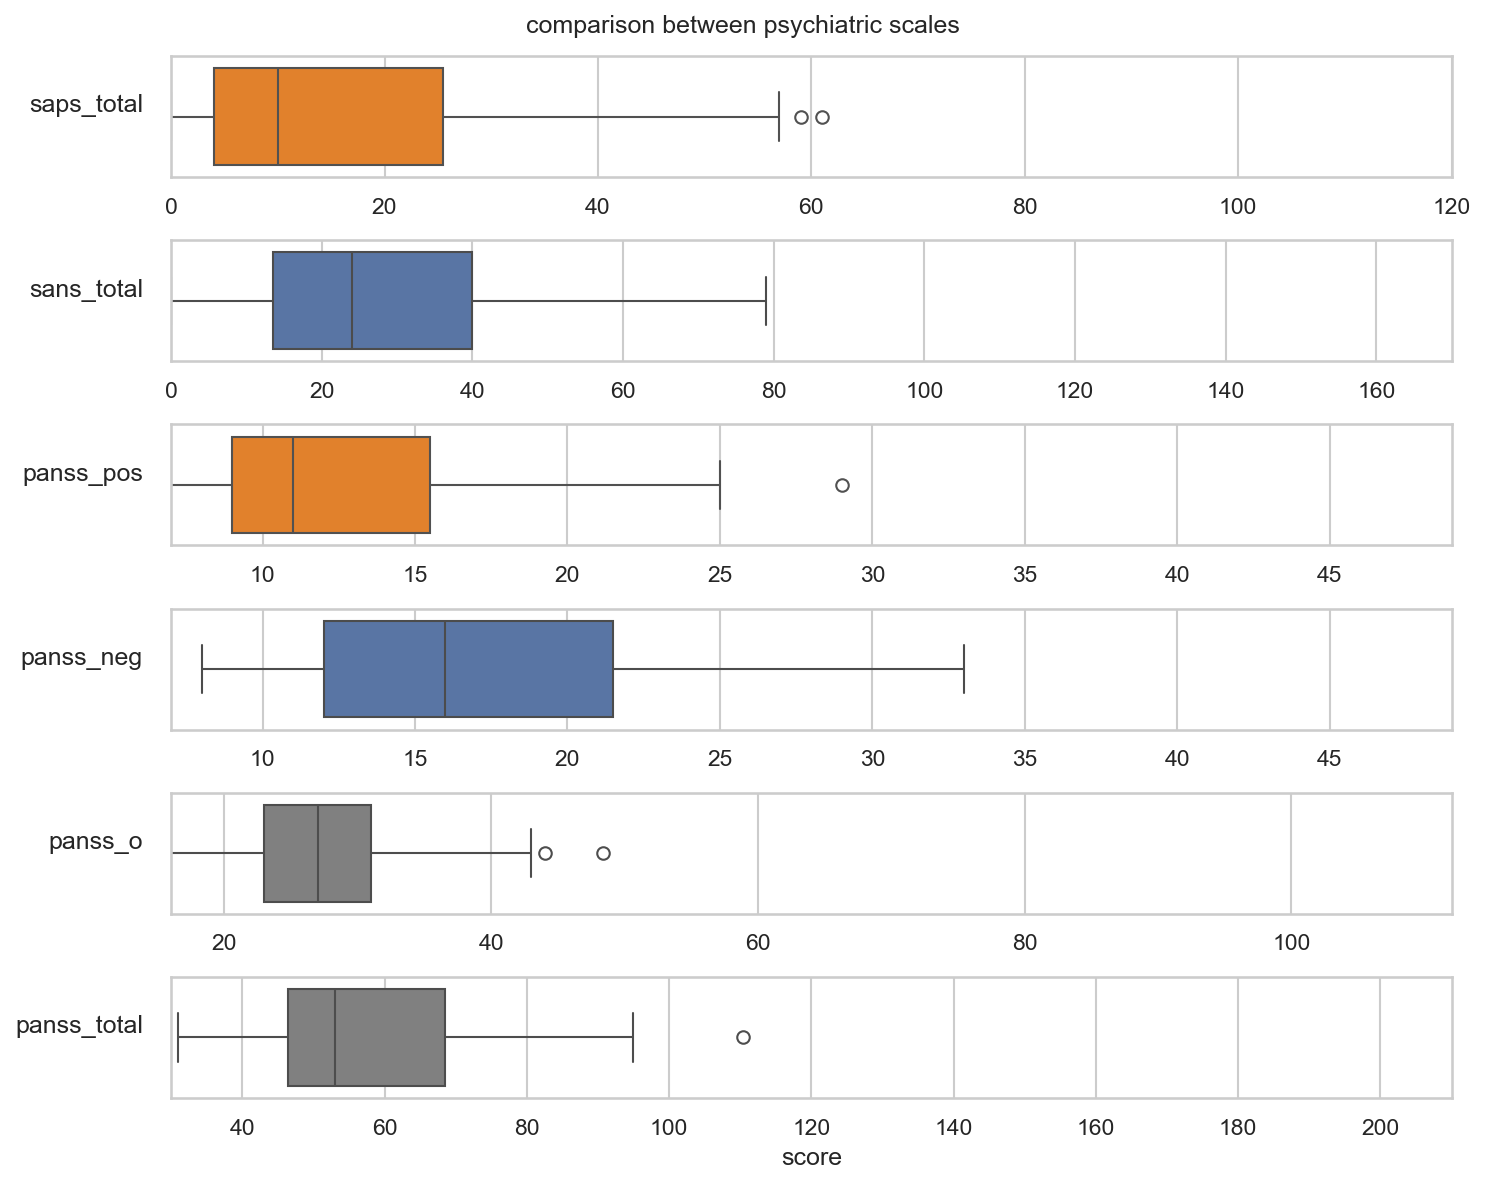
\includegraphics[width=0.6\textwidth]{chapter_3/de_psychiatric.png}  
\captionsetup{width=\textwidth}
\caption[German Clinical Dataset: Psychiatric Scores]{\label{fig:data:de:sample:psy} Clinical statistics of the psychiatric sample in the German clinical dataset. The range corresponds to possible values of the psychiatric scales. Negative symptom scales are shown in blue and positive symptom scales in orange, while grey indicates general symptom scales.}
\end{center}
\end{figure}

\subsection{Russian}
\label{sec:methods:data:clinical:russian}

The Russian clinical sample consisted of monologue speech samples, elicited with 4 tasks, from 31 NAP patients, 18 depressive patients\footnote{The exact diagnosis counts are provided in the appendix \ref{appendix:methods} in table \ref{tab:data:ru:sample:diagnosis}.}, and 30 controls who also underwent a clinical interview process to exclude a possibility of undiagnosed disorders\footnote{The sample partially coincides with the one described in \citet{ryazanskaya2020thesis}. The data was collected jointly by Tatyana Shishkovskaya, Mariya Khudyakova, and me, and transcribed by me. The patient data was collected at the Mental Health Research Center, Moscow.}. 
% , and 102 controls, among whom 30 also underwent a clinical interview process
The sample is characterised in table \ref{tab:data:ru:sample}. There were no differences in age between NAP patients and clinical controls %  (t=2.2, p=0.03)
% ; patients were significantly younger than general controls (t=3.6, p=0.0004)
but there was a significant difference in the years of education between the NAP and control groups (t=3.6, p=0.0006). 
%  and general controls (t=4.7, p=8e-6)
There were no differences between the sexes in any of the samples. It is worth noting that the Russian sample is predominantly female, which is an understudied group when it comes to psychotic disorders, yet this imbalance is a limitation of the present study.

% \begin{table}[h!]
% \begin{center}
% \begin{tabular}{llllll}
% \hline
%     &     & \textbf{N} & \textbf{female} & \textbf{age}  & \textbf{edu\_years} \\ \hline
% NAP &     & 31         & 25              & 27.13 (7.14)  & 13.32 (2.41)        \\
% Dep &     & 18         & 18              & 20.89 (3.71)  & 12.67 (1.94)        \\
% HC  & all & 102 & 75     & 39.75 (19.15) & 15.74 (2.57) \\
%     & psy & 30  & 26     & 25.0 (7.4)    & 15.43 (2.13)        \\ \hline
% \end{tabular}
% \captionsetup{width=\textwidth}
% \caption[Russian Clinical Dataset.]{\label{tab:data:ru:sample} Social statistics of the Russian clinical dataset (only including the participants doing the selected tasks). Standard deviation is provided in parenthesis for each mean value. ``edu\_years'' indicates years of education. ``Dep'' is the sample with predominant depressive symptoms. ``HC psy'' stands for the subset of the healthy patients for which a clinical impression and psychiatric assessment is available.}
% \end{center}
% \end{table}

\begin{table}[ht!]
\begin{center}
\begin{tabular}{lllll}
\hline
    & \textbf{N} & \textbf{female} & \textbf{age}  & \textbf{edu\_years} \\ \hline
NAP & 31         & 25              & 27.13 (7.14)  & 13.32 (2.41)        \\
Dep & 18         & 18              & 20.89 (3.71)  & 12.67 (1.94)        \\
HC  & 30  & 26     & 25.0 (7.4)    & 15.43 (2.13)        \\ \hline
\end{tabular}
\captionsetup{width=\textwidth}
\caption[Russian Clinical Dataset]{\label{tab:data:ru:sample} Social statistics of the Russian clinical dataset (only including the participants doing the selected tasks). Standard deviation is provided in parenthesis for each mean value. ``edu\_years'' indicates years of education. ``Dep'' is the sample with predominant depressive symptoms. ``HC'' stands for the sample of the healthy participants.}
\end{center}
\end{table}

The four tasks used to elicit monologue speech included two picture-elicited tasks (`sportsman' and `adventure'), one instruction task (`chair') and one personal story task (`present')
%\footnote{\textcolor{red}{Other tasks were also available for some of the participants. Only participants who concluded at least one of the four tasks were included in the clinical analysis. \textbf{These texts for the other tasks were used for ...} The description of the entire sample along with the description of other task prompts is provided in \ref{appendix:methods}}}
. The picture description tasks were elicited using two Bidstrup comics, provided in the appendix \ref{appendix:methods}, asking the participant to tell the story depicted in them. The instruction task was elicited using an IKEA chair brochure, asking the participant to instruct a third person, who cannot see the image. Finally, the personal story task was elicited by asking the participant to tell a story about the most memorable present that they had received. As not all participants were able to complete all the tasks, the number of samples available for each task is given in table \ref{tab:data:ru:sample:tasks}. The speech recordings were manually transcribed and separated into sentences according to the same transcription guidelines as the ones used for the German sample. The interviewer's speech, as well as filled hesitation pauses, were removed from the transcripts. 

% \begin{table}[h!]
% \begin{center}
% \begin{tabular}{lllllll}
% \hline
%     &     & N   & adventure & chair & present & sportsman \\ \hline
% NAP &     & 31  & 30        & 17    & 21      & 28        \\
% Dep &     & 18  & 14        & 14    & 13      & 14        \\
% HC  & all & 102 & 55        & 44    & 47      & 54        \\
%     & psy & 30  & 25        & 16    & 19      & 26        \\ \hline
% \end{tabular}
% \captionsetup{width=\textwidth}
% \caption[Russian Clinical Dataset: Task Availability]{\label{tab:data:ru:sample:tasks} Task availability for each selected task in Russian clinical dataset. ``Dep'' is the sample with predominant depressive symptoms. ``HC psy'' stands for the subset of the healthy patients for which a clinical impression and psychiatric assessment is available.}
% \end{center}
% \end{table}

\begin{table}[ht!]
\begin{center}
\begin{tabular}{llllll}
\hline
    & N   & adventure & chair & present & sportsman \\ \hline
NAP & 31  & 30        & 17    & 21      & 28        \\
Dep & 18  & 14        & 14    & 13      & 14        \\
HC  & 30  & 25        & 16    & 19      & 26        \\ \hline
\end{tabular}
\captionsetup{width=\textwidth}
\caption[Russian Clinical Dataset: Task Availability]{\label{tab:data:ru:sample:tasks} Task availability for each selected task in Russian clinical dataset. ``Dep'' is the sample with predominant depressive symptoms. ``HC'' stands for the sample of the healthy participants.}
\end{center}
\end{table}

For each participant, PANSS scores, as well as clinical impressions of thought disorder and depression severity, ranging from 0 to 3, were collected. The scores for each subsample are characterised in table \ref{tab:data:ru:sample:psy}, and figure \ref{fig:data:ru:sample:psy} shows a comparison between the scales in the NAP subsample of the Russian clinical dataset, showing that negative symptoms prevail in this sample. After Bonferroni correction, two of the psychiatric correlated significantly with years of education: PANSS general	(r=-0.41, p\footnote{All p values in this passage are reported as p before correction.}=0.0008) and depression severity (r=-0.33, p=0.003). The psychiatric scores were also intercorrelated. Depression severity correlated with PANSS general (r=0.6, p\textless0.000001) and PANSS total score (r=0.35, p=0.005), as well as thought disorder severity (r=0.33, p=0.003). Thought disorder severity correlated significantly with all other psychiatric scales, most strongly with PANSS positive subscale (r=0.84), total PANSS score (r=0.81), general (r=0.71), and negative (r=0.69) subscales\footnote{All p\textless0.000001.}. All PANSS subscales were significantly intercorrelated with r \textgreater 0.65. 

\begin{table}[ht]
\resizebox{\textwidth}{!}{%
\begin{tabular}{lllllllllllll}
\hline
\textbf{} & \textbf{sex} & \textbf{N} & \textbf{age}                      & \textbf{edu\_years}              & \textbf{Dep} & \textbf{TD} & \textbf{P\_N} & \textbf{PANSS\_TD} & \textbf{PANSS} & \textbf{PANSS\_n} & \textbf{PANSS\_p} & \textbf{PANSS\_o} \\ \hline
range       & & & & & & & &  4-28 & 30-210 & 7-49  & 7-49 & 16-112  \\ \hline
NAP       & all          & 31         & 27.13 (7.14)                      & 13.32 (2.41)                     & 0.58 (0.85)           & 0.84 (0.73)          & 29                        & 10.03 (3.74)       & 69.79 (16.13)  & 22.93 (8.59)        & 15.90 (4.92)        & 30.97 (8.42)      \\ \hline
          & f       & 25         & 27.80 (7.53)                       & 13.56 (2.48)                     & 0.72 (0.89)           & 0.8 (0.76)           & 23                        & 9.43 (3.62)        & 69.13 (15.38)  & 22.52 (7.79)        & 15.3 (4.91)         & 31.3 (9.08)       \\
          & m         & 6          & 24.33 (4.72)                      & 12.33 (1.97)                     & 0.0 (0.0)             & 1.0 (0.63)           & 6                         & 12.33 (3.56)       & 72.33 (20.16)  & 24.5 (11.93)        & 18.17 (4.67)        & 29.67 (5.65)      \\ \hline
Dep       & f       & 18         & 20.89 (3.71)                      & 12.67 (1.94)                     & 0.56 (0.62)           & 0.06 (0.24)          & 13                        & 4.42 (0.9)         & 37.92 (5.89)   & 8.31 (1.97)         & 8.46 (1.94)         & 21.15 (3.58)      \\ \hline
HC & all    & 30 & 25.0 (7.4)   & 15.43 (2.13) & 0.0 (0.0)   & 0.0 (0.0)   & 22   & 4.36 (1.0)   & 30.77 (1.54)  & 7.23 (0.53)  & 7.23 (0.61)  & 16.32 (0.95) \\ \hline
         & f & 26 & 25.42 (7.8)  & 15.42 (1.7)  & 0.0 (0.0)   & 0.0 (0.0)   & 20   & 4.4 (1.05)   & 30.85 (1.6)   & 7.25 (0.55)  & 7.25 (0.64)  & 16.35 (0.99) \\
         & m   & 4  & 22.25 (3.3)  & 15.5 (4.43)  & 0.0 (0.0)   & 0.0 (0.0)   & 2    & 4.0 (0.0)    & 30.0 (0.0)    & 7.0 (0.0)    & 7.0 (0.0)    & 16.0 (0.0)  \\ \hline
\end{tabular}
}
\captionsetup{width=\textwidth}
\caption[Russian Clinical Dataset: Psychiatric Scores]{\label{tab:data:ru:sample:psy} Clinical statistics of the psychiatric sample in the Russian clinical dataset (only including the participants doing the selected tasks). ``HC'' only refers to the subset of the healthy patients. Standard deviation is provided in parenthesis for each mean value. The range is provided for the possible values of the psychiatric scales. \\ ``f'' stands for female; ``m'' for male. ``edu\_years'' indicates years of education; ``P\_N'' indicates the number of participants for whom PANSS scores are available, ``PANSS\_td'' stands for the sum for PANSS questions related to formal thought disorder.}
\end{table}

\begin{figure}[ht!]
\begin{center}
    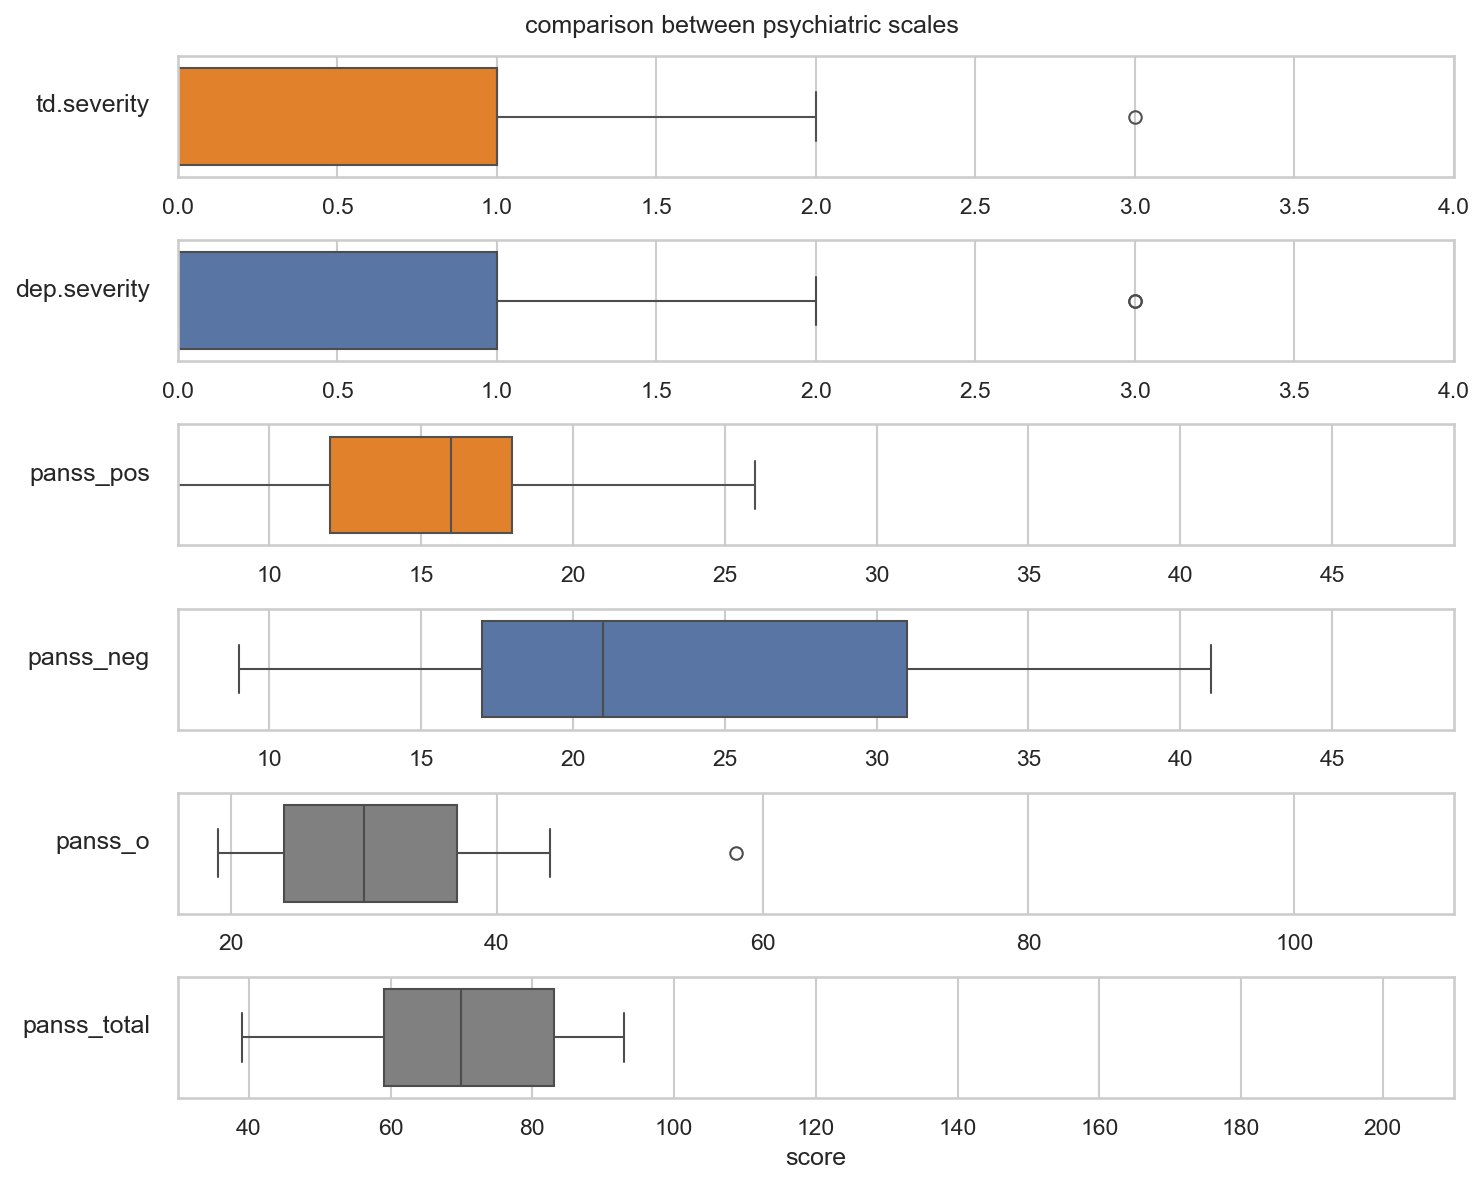
\includegraphics[width=0.6\textwidth]{chapter_3/ru_psychiatric.png}  
\captionsetup{width=\textwidth}
\caption[Russian Clinical Dataset: Psychiatric Scores]{\label{fig:data:ru:sample:psy} Clinical statistics of the psychiatric sample in the NAP subsample of the Russian clinical dataset. The range corresponds to possible values of the psychiatric scales. Negative symptom scales are shown in blue and positive symptom scales in orange, while grey indicates general symptom scales.}
\end{center}
\end{figure}


%-----------------------------------
%	section 2
%-----------------------------------
\section{Data Processing: Metric Pool}
\label{sec:methods:processing:metrics}

Each text in the clinical sample was automatically separated into sentences based on punctuation, tokenised, and lemmatised. The selected metrics, described below, were then computed for each text separately. 

\subsection{Lexical Methods}
As there was little consistency in the use of semantic lexical metrics, only the Lemma-Token Ratio (LTR), Moving Average Lemma-Token Ratio (MALTR), and total word count (n words) were used. LTR was computed as the total number of unique lemmas over the total word count. MALTR was computed as LTR averaged across a moving window of size 10\footnote{The window size was selected to be close to mean sentence length.}, with overlapping windows shifting one word at a time regardless of sentence boundaries. The lemmatization was performed using the SpaCy\footnote{Spacy version 3.7.2.} \texttt{de\_core\_news\_md} and \texttt{ru\_core\_news\_md} models.

\subsection{Syntactic Methods}
The syntactic metrics included sentence parameters such as mean, maximal, and minimal sentence length, along with standard deviation in sentence length, and total sentence count (n sents). Additionally, part-of-speech (POS) rates were used for the POS tested previously: adjectives (ADJ), adverbs (ADV), auxiliary verbs (AUX), coordinating and subordinating conjunctions (CCONJ, SCONJ), determiners (DET), nouns and proper nouns (NOUN, PRPON), pronouns (PRON), particles (PART), and verbs (VERB). The POS tagging was performed using SpaCy models, and the rate was computed as the number of instances of a particular part-of-speech over the total word count.

\subsection{Graph-Based Methods}
The graphs were constructed based on word co-occurrence, as done in \citet{mota2012speech}. The graph construction was performed over lemmas and was performed over a moving window of 100 words\footnote{The moving average approach to graph methods is commonly accepted, and though the window size is not always reported, the 100 words is a common window size. Only few texts were below 100 words in total.}. A pair of lemmas was connected with a directed edge every time they appeared one after the other. The graph metrics included the number of nodes (N)\footnote{The number of nodes corresponds to the unique lemma count calculated over a moving window of size of 100.}, number of edges (E), largest connected component (LCC), largest strongly connected component (LSC), number of parallel edges (PE), number of loops of length one (repeated words), two, and three (L1, L2, L3), average node degree, and standard deviation in the node degree. These characteristics were computed for each window graph and then averaged across the overlapping windows. The characteristics of the graphs were computed using the \texttt{networkx} library.

\subsection{Language Model-Based Methods}
For LM-based methods, three models were compared. First, word2vec, which was loaded via SpaCy interface (obtained from \href{https://fasttext.cc/docs/en/crawl-vectors.html}{fasttext}\footnote{https://fasttext.cc/docs/en/crawl-vectors.html} for \texttt{de} and \texttt{ru})\footnote{Fasttext models at \href{https://fasttext.cc/docs/en/crawl-vectors.html}{fasttext website} are all pretrained on common crawl and Wikipedia dumps.}. Second, built-in SpaCy GloVe models (\texttt{de\_core\_news\_md} and \texttt{ru\_core\_news\_md}). Finally, BERT sentence embeddings (\texttt{bert-base-german-cased} for German and  \texttt{DeepPavlov/rubert-base-cased} for Russian). The two simplest methods of obtaining sentence embeddings from word embeddings were compared for word2vec: simple averaging word vectors (\texttt{w2v\_avg} and \texttt{glove\_avg}) and TF-IDF weighted averaging of word vectors (\texttt{w2v\_tf} and \texttt{glove\_tf}). The word frequencies for TF-IDF were obtained from the \texttt{wordfreq} library\footnote{wordfreq version 3.1.1}. The TF-IDF weighting for word averaging implied giving each word vector a weight of one over the looked-up corpus word frequency, and the `term frequency' was accounted for by the repetition of the word vectors where they were repeated in the sentence. The `CLS' token embedding was used as the BERT sentence vector representation.

Each model sentence vectors were used to compute several coherence scores, namely, local (first order) coherence (\texttt{lcoh}), second order coherence (\texttt{scoh}), global coherence (\texttt{gcoh}) and cumulative global coherence (\texttt{cgcoh}). Local coherence was computed as the mean cosine similarity between the pairs of consecutive sentence vectors. Second-order coherence was computed as the mean cosine similarity between the pairs of sentence vectors with one intervening sentence between them. Global coherence was computed as the mean cosine similarity between each sentence vector and the mean vector of all sentences. Finally, cumulative global coherence was computed as the mean cosine similarity between each sentence vector and the mean vector of all preceding sentences.

A separate representation of the same BERT model was used to estimate pseudo-perplexity (\texttt{pppl}). It was obtained by masking one word at a time and obtaining the pseudo log-likelihood of the word that was masked for each word in a sentence. The pseudo log-likelihoods were then averaged across the sequence and exponentiated to obtain a pseudo-perplexity score\footnote{The calculation was simplified by \href{https://huggingface.co/docs/transformers/perplexity}{passing the true input token ids as labels to the model}, and the loss was simply exponentiated, thus calculating the average masking pseudo log-likelihood for each token in the sentence in one line.}. The metric was averaged across all sentences.

Finally, a separate BERT representation was used to obtain next sentence probability scores for each pair of consecutive sentences (\texttt{sprob}), and the metric was averaged across all sentence pairs. 

\section{Data Analysis}
\label{sec:methods:stats:clinical}

\subsection{Control Variables}
Both samples were analyzed using a two-sided independent t-test for between-group differences in the psycho-social characteristics, as well as for any effects of sex within each group. The psychiatric scales were analyzed for the degree of inter-correlation, as well as for age, education years, and IQ (using Pearson's r). To rule out the effect of age, education years, and IQ, the correlation of the tested metrics with them was computed. Additionally, the correlation of each psycho-social variable with mean sentence length was analyzed to account for results that could stem from the differences in mean sentence length.

\subsection{Target Variables}
Bootstrap was used to evaluate the uncertainty of each metric performance estimate and to account for the effect of the influential points. The data points were drawn with replacements from the sample until the actual sample size was reached; then, the performance was estimated on this sample. For each metric, median value and 25/75 percentiles were used to estimate the metric performance across 1000 iterations.

The performance of each metric was assessed using:
\begin{itemize}
    \item two-sided independent t-test for between-group differences\footnote{The t-test was computed using \texttt{scipy.stats} (version 1.9.1).}. %For the Russian clinical sample, only clinical controls were used in t-test.};
    \item Pearson's r correlation with each psychiatric scale\footnote{The Pearson's r was also computed using \texttt{scipy.stats}.};
    \item ordered categorical regression McFadden’s pseudo r squared for TD and depression severity variables\footnote{The ordered model provided in \texttt{statsmodels} (version 0.13.5) was used.};
    \item Pearson's r correlation with mean sentence length to control for effects explained merely by differences in sentence length.
\end{itemize}

The p-values were not analyzed for the bootstrap, as only the point of the present work is to assess the relative rather than the absolute performance of the metrics\footnote{Due to multiple comparisons, very few if any metrics would remain significant in this benchmark study.}. A metric was considered well-performing if it correlated above 0.3 with any psychiatric scale or had pseudo r squared above 0.09. For the t-test, the metric was well-performing if the 25-75 percentile interval did not cross zero. The metric was considered to be length-dependent if it correlated with mean sentence length above 0.3, yet metrics outperforming the mean sentence length baseline were still considered of interest and analyzed. All were compared for their performance on different psychiatric scales, and for the Russian clinical sample, the metrics were additionally compared for their performance on different tasks. Then the results were compared across languages.


% %----------------------------------------------------------------------------------------
% %	SECTION 2
% %----------------------------------------------------------------------------------------
% \section{Corpus Analysis}
% %-----------------------------------
% %	section 1
% %-----------------------------------
% \section{Spoken Corpus Data}
% \subsection{German}
% \textcolor{red}{DGD}
% \subsection{Russian}
% \textcolor{red}{RusCorpora}


% %-----------------------------------
% %	section 2
% %-----------------------------------
% \section{Web Corpus Data}
% \subsection{German}
% \subsection{Russian}
% \textcolor{red}{Wiki?}


% %-----------------------------------
% %	section 3
% %-----------------------------------
% \section{Corpus Data Processing}
% \label{sec:methods:processing:corpus}
% \textcolor{red}{same metric pool};
% \textcolor{red}{preprocessing, metric application, nan averaging}

% %-----------------------------------
% %	section 4
% %-----------------------------------
% \section{Corpus Data Analysis}
% \label{sec:methods:stats:corpus}

% \textcolor{red}{statistical comparisons?}

% Chapter Template

\chapter{Results}
\label{chap:4:results}

\label{sec:results:clinical}

In this chapter, I first discuss the textual characteristics of both samples and verbosity patterns (\ref{sec:results:clinical:sample_length}), then turn to the interaction between the social variables and the target variables, as well as the relation between the target variables and the text length (\ref{sec:results:clinical:control_variables}). Afterwards, each group of metrics is discussed separately for both languages (\ref{sec:results:clinical:lexical}-\ref{sec:results:clinical:LM}). Finally, I present a cross-group (\ref{sec:results:clinical:cross_group}) and a cross-linguistic (\ref{sec:results:clinical:cross_linguistic}) comparison of the studied metrics.

%-----------------------------------
%	section 1
%-----------------------------------
\section{Textual Characteristics of the Samples}
\label{sec:results:clinical:sample_length}

As NAP patients are believed to be less verbose, it is important to take the differences in text length into account. Table \ref{tab:data:length} summarizes the length characteristics of both German and Russian samples. Unlike what has been reported previously, the overall text length, i.e. word count, seems to be explained more by the number of sentences than by their length, though sentence length also plays some role, especially in the German sample. It also seems to play some role in the overall verbosity on two of the tasks in the Russian sample, adventure and chair, - the shortest and the longest one, respectively. 

Figures \ref{fig:data:de:length} and \ref{fig:data:ru:length} show the relation between the word count and both sentence count and mean sentence length, as well as the correlation coefficient, underlining the differences in the components contributing to the text length across the tasks and languages. These differences imply that the mean sentence length would serve as a strong baseline for performance only on some tasks, while on others only the number of sentences, and, possibly, the word count, would function as such. For the tasks, where the differences in mean sentence length are prominent, it is especially important to account for the intrinsic relation between some of the metrics and mean sentence length. However, no such correction is required for the number of sentences, as there seems no intrinsic relation between the number of sentences and the metric values for any of the metrics used, except the verbosity\footnote{It is possible that the moving window procedure does not entirely remove the effects of verbosity from the graph-based metrics. These effects may come via the number of sentences, rather than sentence length, though with the latter the graph-based metrics are indeed not intrinsically related. Yet, we do not explore this question further in the present work.}.

\begin{table}[h]
\resizebox{\textwidth}{!}{%
\begin{tabular}{llllll}
\hline
\textbf{} & \textbf{German} & \textbf{Russian} & \textbf{} & \textbf{} & \textbf{} \\
\textbf{task} & \textbf{} & \textbf{adventure} & \textbf{chair} & \textbf{present} & \textbf{sportsman} \\ \hline
n words           & \begin{tabular}[c]{@{}l@{}}184.2\\ (117.4)\end{tabular} & \begin{tabular}[c]{@{}l@{}}129.8 \\ (82.1)\end{tabular} & \begin{tabular}[c]{@{}l@{}}168.4 \\ (120.9)\end{tabular} & \begin{tabular}[c]{@{}l@{}}140.8 \\ (107.7)\end{tabular} & \begin{tabular}[c]{@{}l@{}}134.4 \\ (86.0)\end{tabular} \\
n sents & 17.9 (9.3) & 18.7 (11.0) & 20.4 (15.0) & 15.1 (12.7) & 17.7 (10.1) \\
mean sent len & 10.0 (2.8) & 6.9 (1.5) & 8.1 (1.6) & 9.9 (4.7) & 7.8 (2.2) \\
r n sents & 0.88 & 0.93 & 0.95 & 0.95 & 0.93 \\
r n mean sent len & 0.59 & 0.36 & 0.38 & 0.08 & 0.11 \\ \hline
\end{tabular}
}
\captionsetup{width=\textwidth}
\caption[Text Length Characteristics]{\label{tab:data:length} Statistics of the mean length of each task between the languages. Standard deviation is provided in parenthesis for each mean value. \\ `n words' stands for the word count, `n sents' for sentence count, and `mean sent len' for mean sentence length. `r n sents' indicates the correlation coefficient of the word count with the sentence count and `r mean sent length' that of the word count with mean sentence length.}
\end{table}

\begin{figure}[ht!]
\begin{center}
    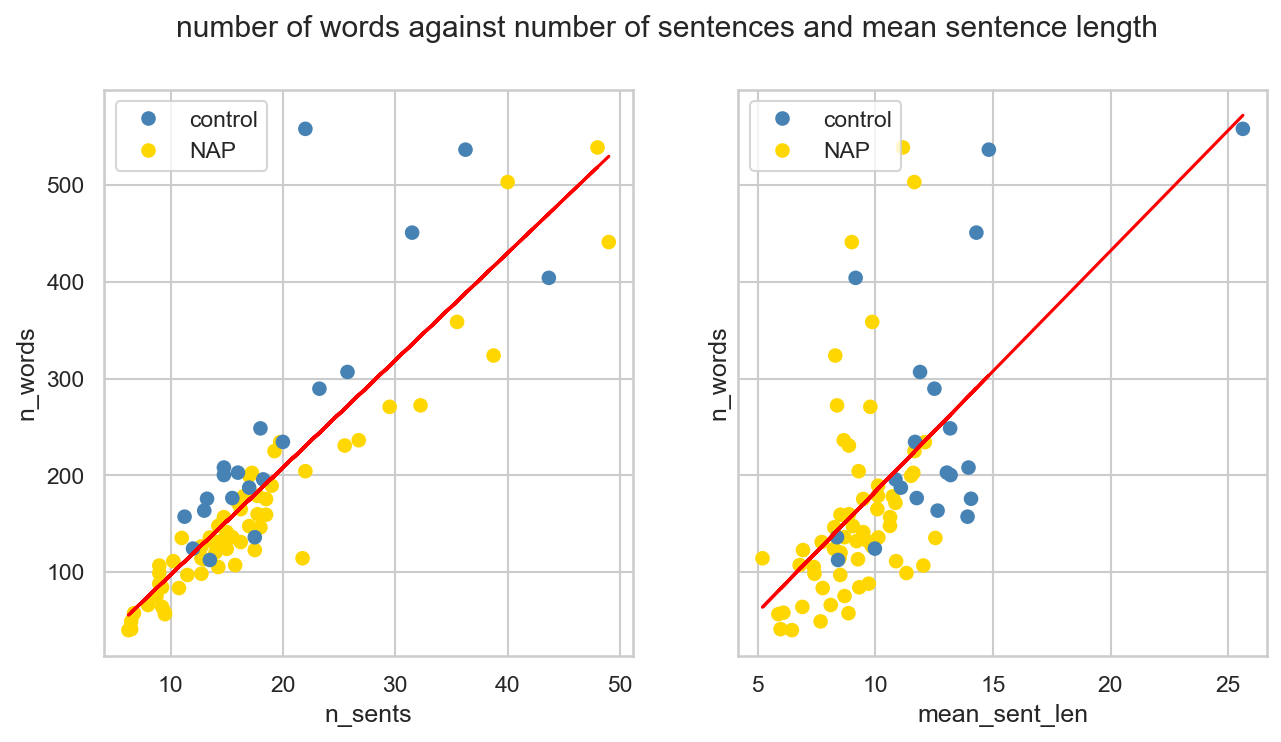
\includegraphics[width=0.7\textwidth]{Figures/chapter_4/de_n_words_n_sents.png} 
\caption[German Clinical Dataset: Length Characteristics]{\label{fig:data:de:length} The correlation between word count and both sentence count and mean sentence length on the German sample, with colors indicating controls and NAP groups.}
\end{center}
\end{figure}

\begin{figure}[p]
\begin{center}
    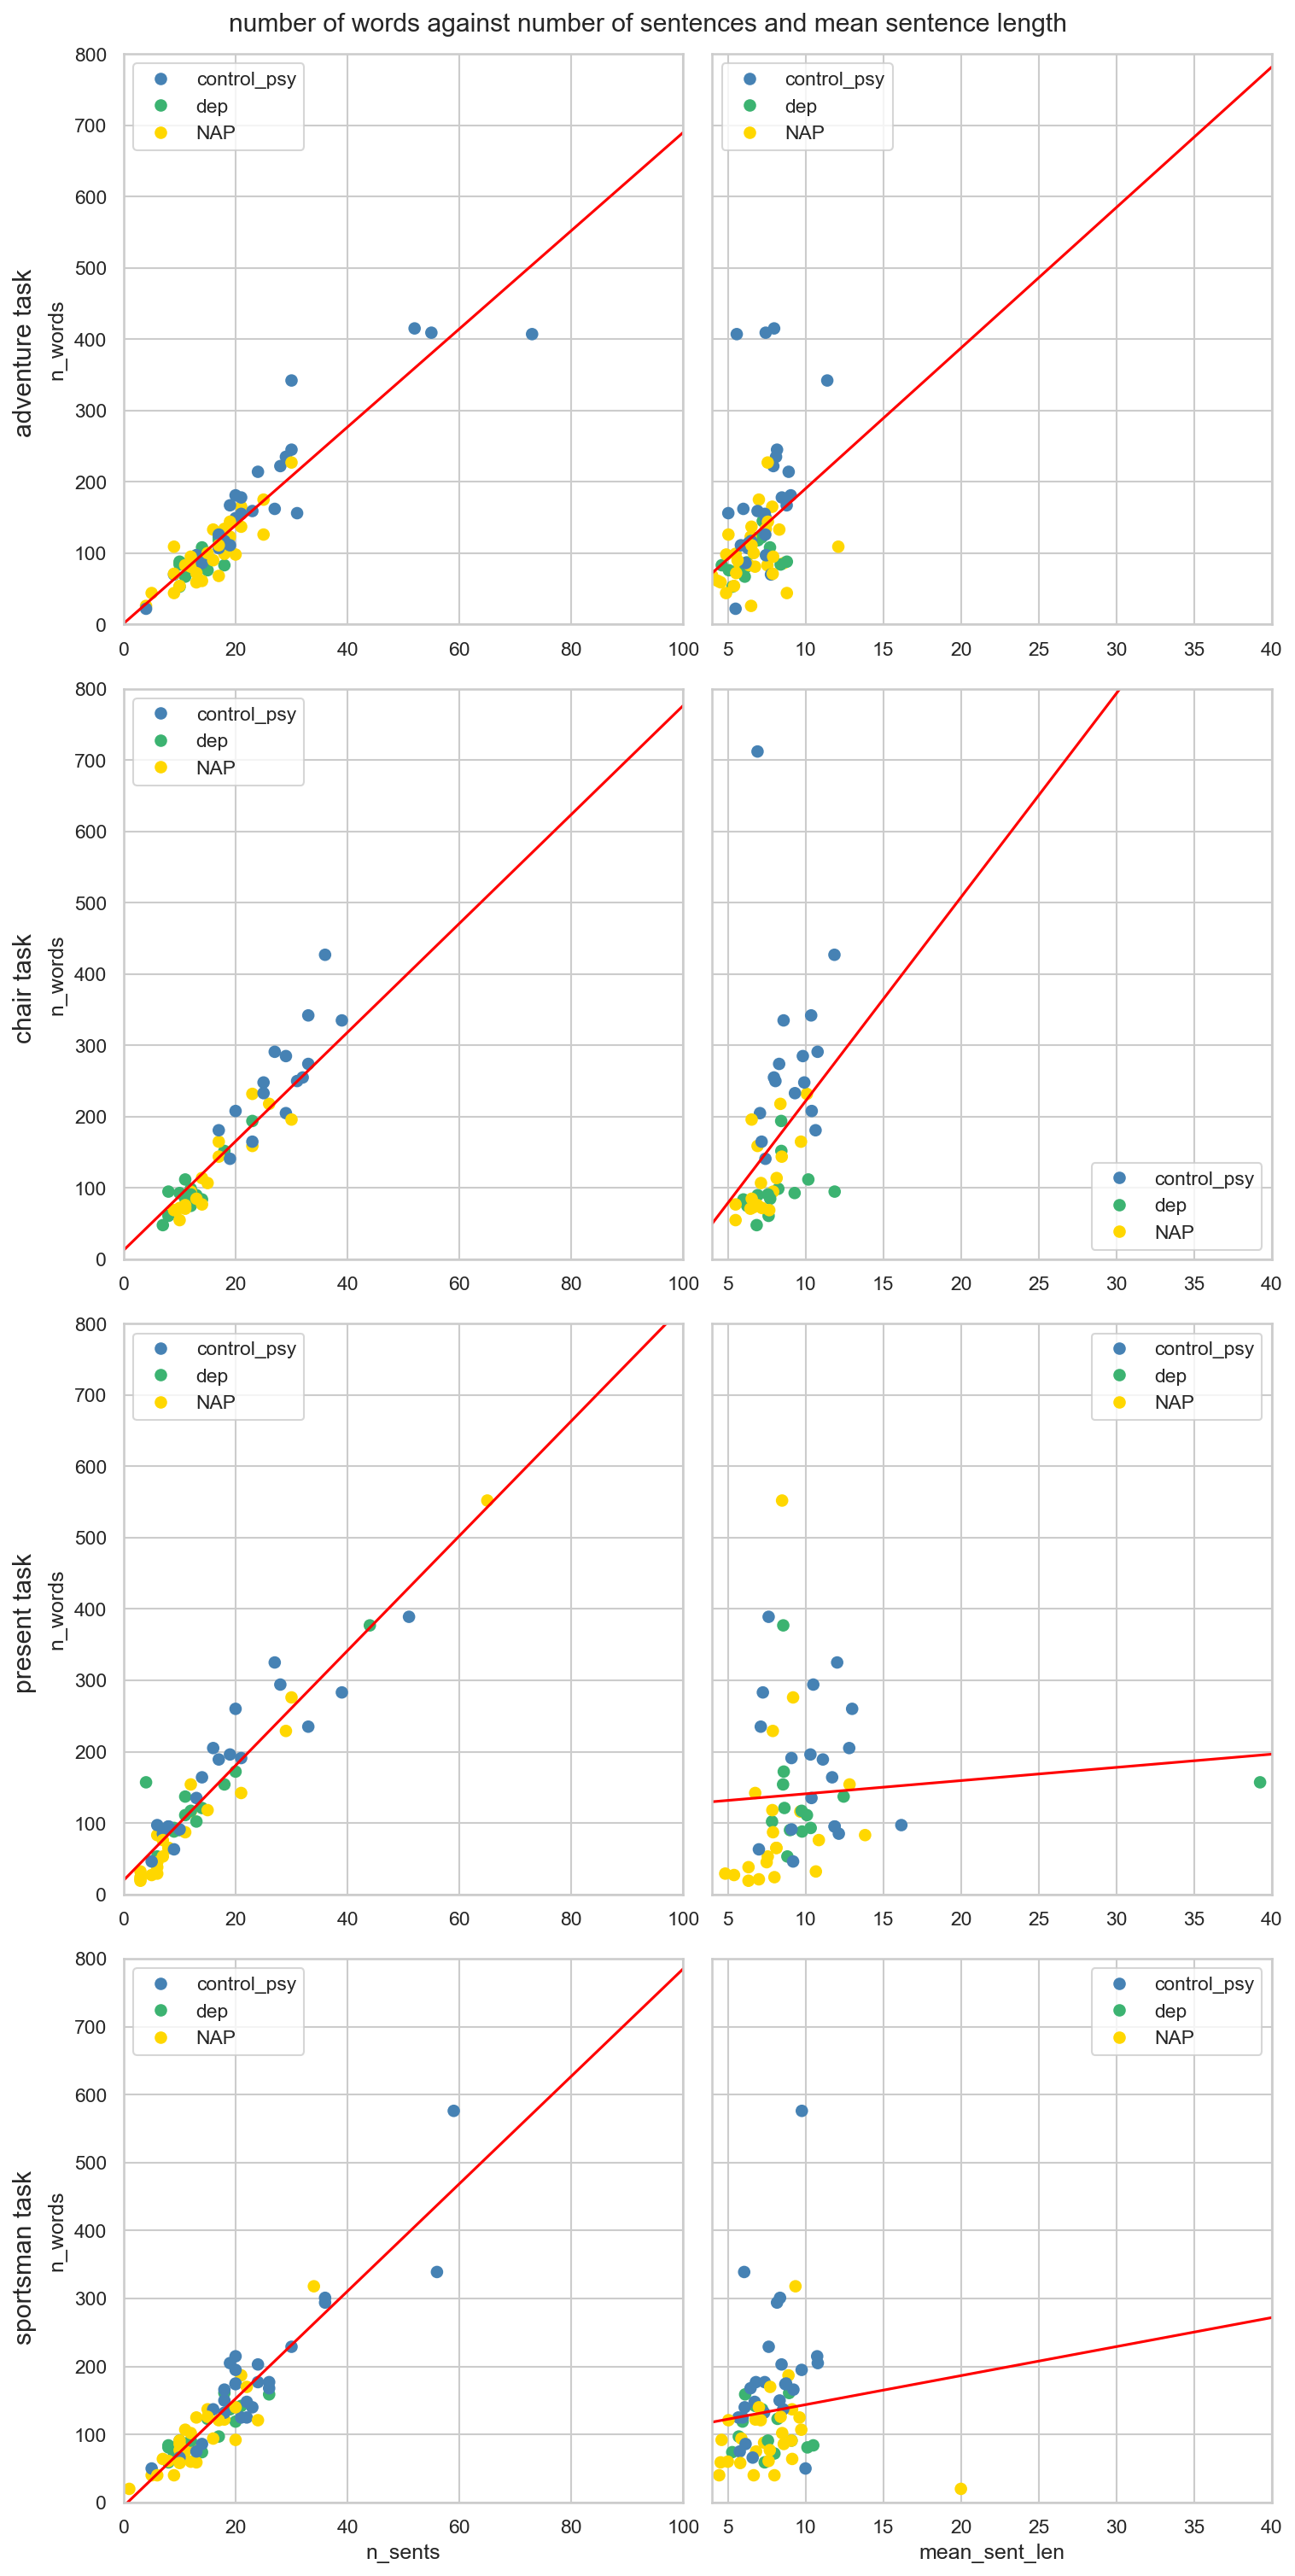
\includegraphics[width=0.7\textwidth]{Figures/chapter_4/ru_n_words_n_sents.png} 
\caption[Russian Clinical Dataset: Length Characteristics]{\label{fig:data:ru:length} The correlation between word count and both sentence count and mean sentence length on the Russian sample for each of the tasks, with colors indicating controls, depression and NAP groups.}
\end{center}
\end{figure}

\pagebreak



%-----------------------------------
%	section 2
%-----------------------------------
\section{Control Variables}
\label{sec:results:clinical:control_variables}

\subsection{German}

After correcting for multiple testing, there remained a significant negative correlation of symptom severity with mean sentence length for negative symptom scales: SANS and PANSS negative (r \textless -0.4, p before correction \textless 0.001). There was no relation between sentence length and sex, age, years of education, or verbal IQ. 

As for the relation between the control variables and the tested metrics, there was no difference in metric between the sexes, and no significant correlation with age, years of education, or verbal IQ, after Bonferroni correction.

\subsection{Russian}

After correcting for multiple testing, there was no significant correlation with mean sentence length for any of the psychiatric scales or social variables, though this may be both because of a high number of comparisons and a lower importance of mean sentence length for overall word count in the Russian sample. 

There also was no correlation between the metrics and the control variables, after controlling for multiple comparisons, with no significant correlation with age or ears of education, and no effect of sex, though here as well it may be due to a high number of comparisons.


%-----------------------------------
%	section 3
%-----------------------------------
\section{Scale and Task Effects}

Table \ref{tab:results:scales_tasks} summarizes the performance of the tested metrics across tasks and scales, showing the number of metrics correlated with each psychiatric scale, as well as the number of metrics among them which were also uncorrelated with mean sentence length.

\begin{table}[ht]
\resizebox{\textwidth}{!}{%
\begin{tabular}{lllllll}
\hline
    & \textbf{German}     & \textbf{Russian}   &        &         &           &         \\
    & \textbf{total (De)} & \textbf{adventure} & \textbf{chair}  & \textbf{present} & \textbf{sportsman} & \textbf{total (Ru)} \\ 
\hline
\textbf{PANSS total}  & 16 (3)    & 9 (2)     & 12 (5) & 18 (13) & 8 (7)     & 30 (17) \\
\textbf{PANSS\_pos}   &  1 (0)    & 1 (1)     & 12 (5) & 13 (11) & 10 (8)    & 24 (15) \\
\textbf{PANSS\_neg}  & 12 (3)      & 8 (1)     & 5 (3)  & 17 (12) & 8 (7)     & 28 (15) \\
\textbf{PANSS\_o}    & 14 (2)      & 7 (2)     & 11 (4) & 18 (13) & 7 (6)     & 28 (16) \\
\textbf{SANS}        & 10 (3)      & -         & -      & -       & -         & -       \\
\textbf{SAPS}         & 5 (1)     & -         & -      & -       & -         & -       \\
\textbf{dep severity} & -         & 0 (0)     & 9 (2)  & 0 (0)   & 0 (0)     & 9 (2)   \\
\textbf{td severity}  & -         & 0 (0)     & 3 (2)  & 13 (11) & 4 (3)     & 19 (15) \\ 
\hline
\textbf{total }       & 21 (4)    & 10 (2)     & 17 (5) & 23 (18) & 10 (8)    & 30 (20)    \\ 
\hline
\end{tabular}
}
\captionsetup{width=\textwidth}
\caption[Scale and Task Effects]{\label{tab:results:scales_tasks} The number of metrics correlating above 0.3 with the target scale (or having pseudo r squared above 0.9) and either do not correlate with mean sentence length above the threshold of 0.3 or outperform this baseline metric. In parenthesis are the numbers of metrics not correlating with sentence length above 0.3.}
\end{table}

\subsection{German}
The overall differences between the scales are summarized in table \ref{tab:results:scales_tasks}. On the German sample, negative symptoms predominate, and, therefore, across the tested metrics, the correlation with the negative symptoms is stronger than with the positive. Additionally, SAPS, which is dedicated solely to the positive symptoms, was more detailed than the corresponding PANSS subscale. Thus, the correlation with SAPS across the metrics was stronger than with the positive PANSS subscale. Yet, SANS and PANSS negative subscale were close to each other. The total PANSS score, as it encompasses both positive and negative symptoms, was correlated with most metrics. On the German sample, the correlation with mean sentence length was frequent for the well-performing metrics, yet many metrics outperformed this baseline. As for the group differences in the metrics on the German sample, they are discussed below for each metric type. 

\subsection{Russian}
The same table (\ref{tab:results:scales_tasks}) shows the overall effects of both tasks and scales for the Russian sample. On it, negative symptoms also predominate, and across all PANSS subscales, the symptoms are more severe than in the German sample. Thus, both positive and negative, as well as general symptoms correlated with some of the metrics. Like on the German sample, PANSS total score correlated with most metrics, however, all PANSS subscales followed closely, the positive symptoms being hardest to predict. TD severity was slightly more less predictable, being easiest to predict on one of the tasks (present), and depression severity could only be predicted on one task (chair). No metric was sensitive enough to reliably differentiate between the groups on the Russian sample, as all bootstrap quantile-based error bars crossed zero for all tasks and metrics\footnote{Due to this absence of any meaningful difference between the groups, the t-test results for the Russian sample are not discussed in any more detail in the present work.}.

The symptom severity was most strongly correlated with the metrics calculated on present task, followed by chair task, sportsman task, and adventure task. This means that the two picture-elicited tasks, sportsman and adventure, were the hardest to predict the symptom severity on. 

As verbosity was more explained by mean sentence length for chair and adventure tasks, these two showed the most difference between the metrics that did not correlate with sentence length and those that did but outperformed it. On the other two tasks, the sentence length did not serve as a strong baseline and the aforementioned difference was therefore not as pronounced.


%-----------------------------------
%	section 4
%-----------------------------------
\section{Lexical Methods}
\label{sec:results:clinical:lexical}
This section covers the performance of the selected lexical metrics, namely, lemma-token ratio (LTR), moving average lemma-token ratio (MALTR), and word count (n words) across target variables in both languages.

\subsection{German}
Figure \ref{fig:results:lexical:de} shows the performance of each lexical metric on SANS, SAPS, and PANSS subscales. On the German sample, LTR positively correlated with the negative symptom scales (PANSS negative and SANS), total PANSS, and PANSS general subscale. MALTR, on the other hand, weakly negatively correlated with both SANS and SAPS. Finally, word count negatively correlated with the negative symptom scales.

\begin{figure}[h!]
    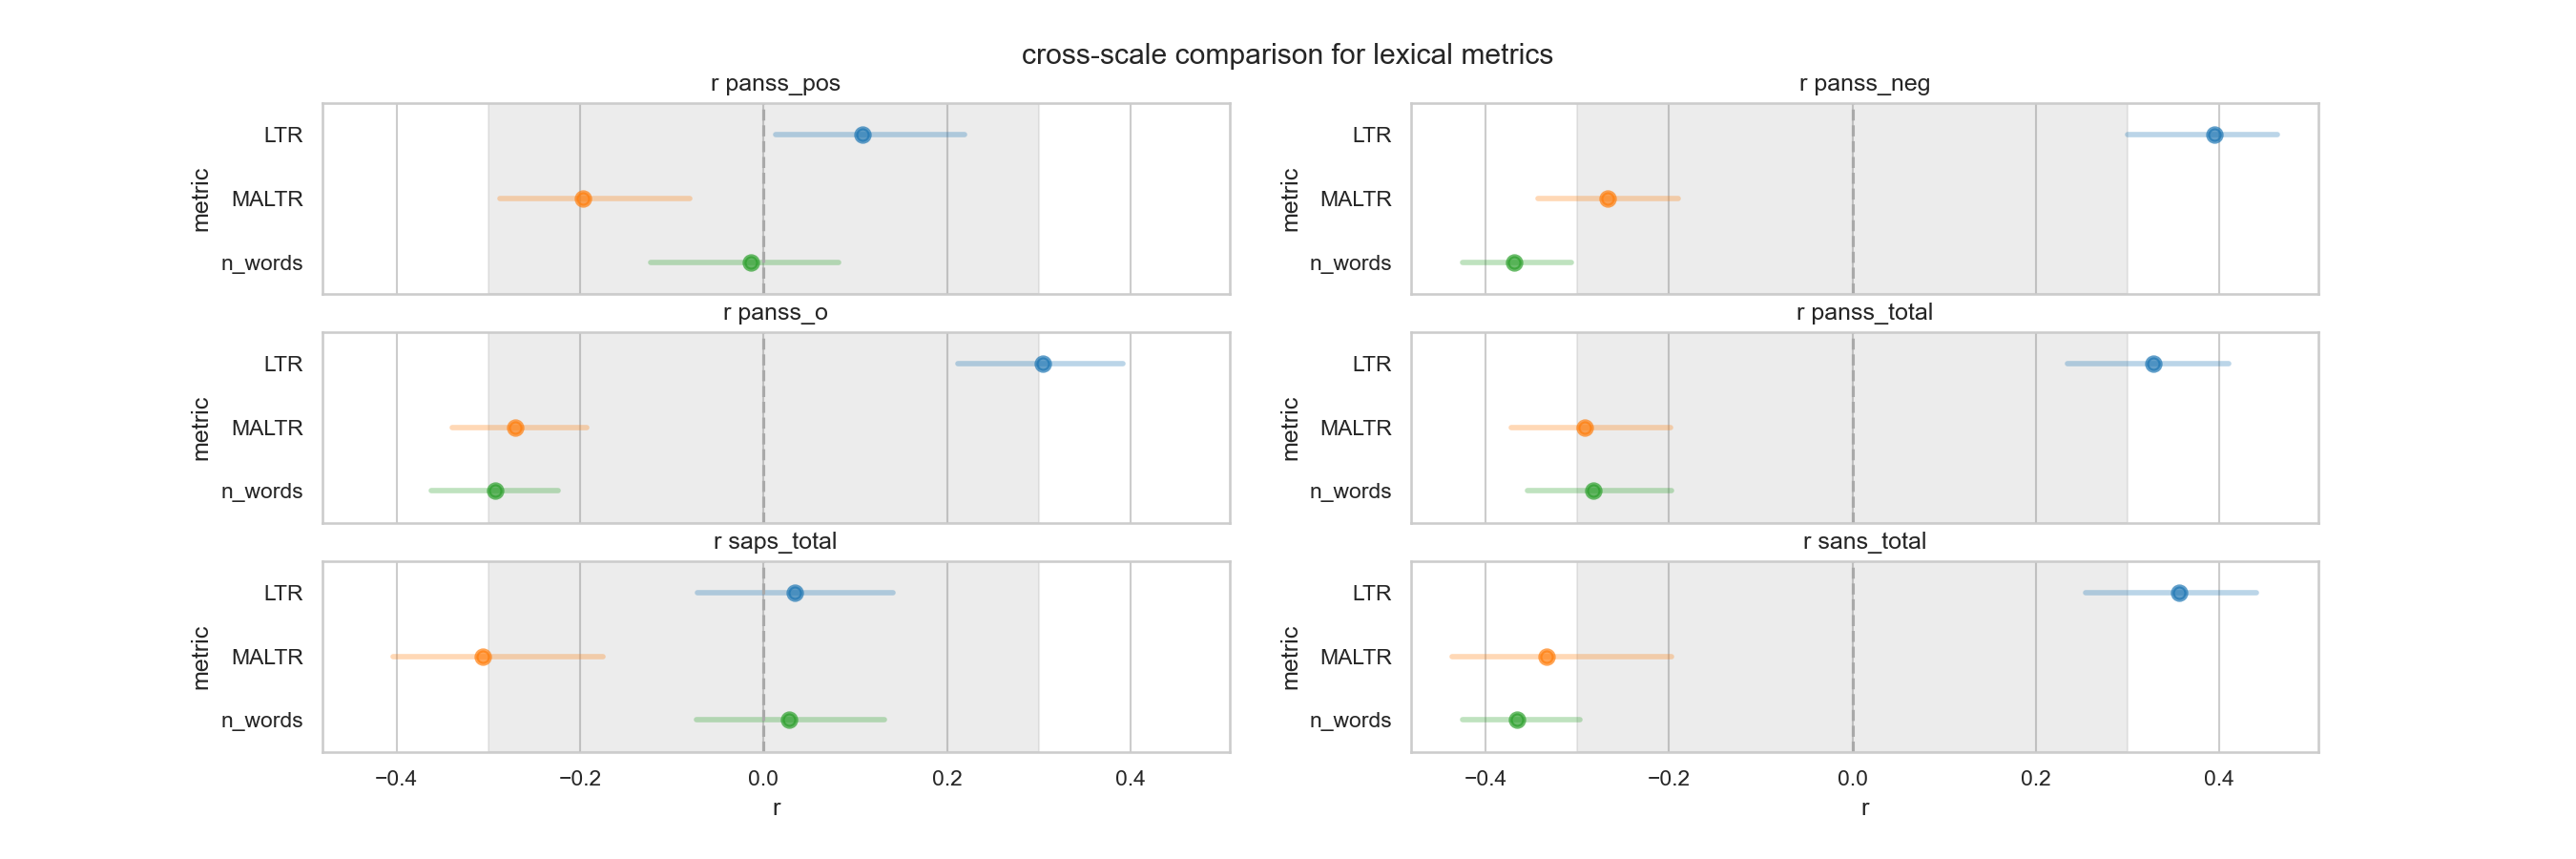
\includegraphics[width=1.2\textwidth, center]{Figures/chapter_4/lexical/de_scale_r.png} 
\captionsetup{width=\textwidth}
\caption[Lexical Metrics: German]{\label{fig:results:lexical:de} Pearson's r correlation coefficient with each scale for the lexical metrics on the German dataset. Grey indicates the values below the 0.3 threshold in absolute value.}
\end{figure}

As shown in figure \ref{fig:results:lexical:de:ttest}, the correlation with mean sentence length closely matched the performance of each metric on the t-test. The LTR was higher in the patient group, while the word count was lower, with no difference in MALTR. All three metrics correlated with mean sentence length, LTR negatively, and MALTR and word count positively.

\begin{figure}[ht!]
    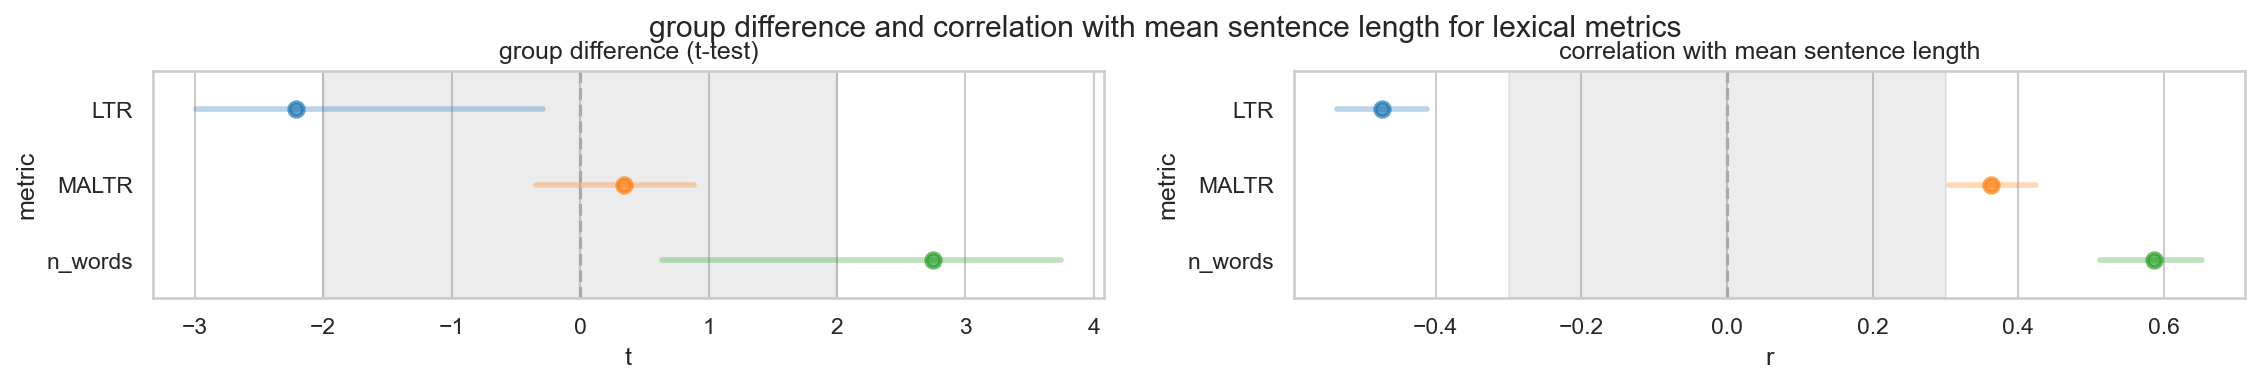
\includegraphics[width=\textwidth, center]{Figures/chapter_4/lexical/de_t_test_corr_len.png} 
\captionsetup{width=\textwidth}
\caption[Lexical Metrics: German (T-Test)]{\label{fig:results:lexical:de:ttest} T-test and Pearson's r correlation coefficient with mean sentence length for the lexical metrics on the German dataset. Grey indicates the values below 2 for the t score and below the 0.3 threshold in absolute value for the correlation coefficient.}
\end{figure}


\subsection{Russian}
On adventure task, shown in figure \ref{fig:results:lexical:ru:ad}, LTR did not perform on any of the scales. MALTR correlated negatively with PANSS negative and general scales, as well as the total PANSS score. Word count correlated negatively with all PANSS scales. None of the metrics could detect TD or depression severity.

\begin{figure}[ht!]
    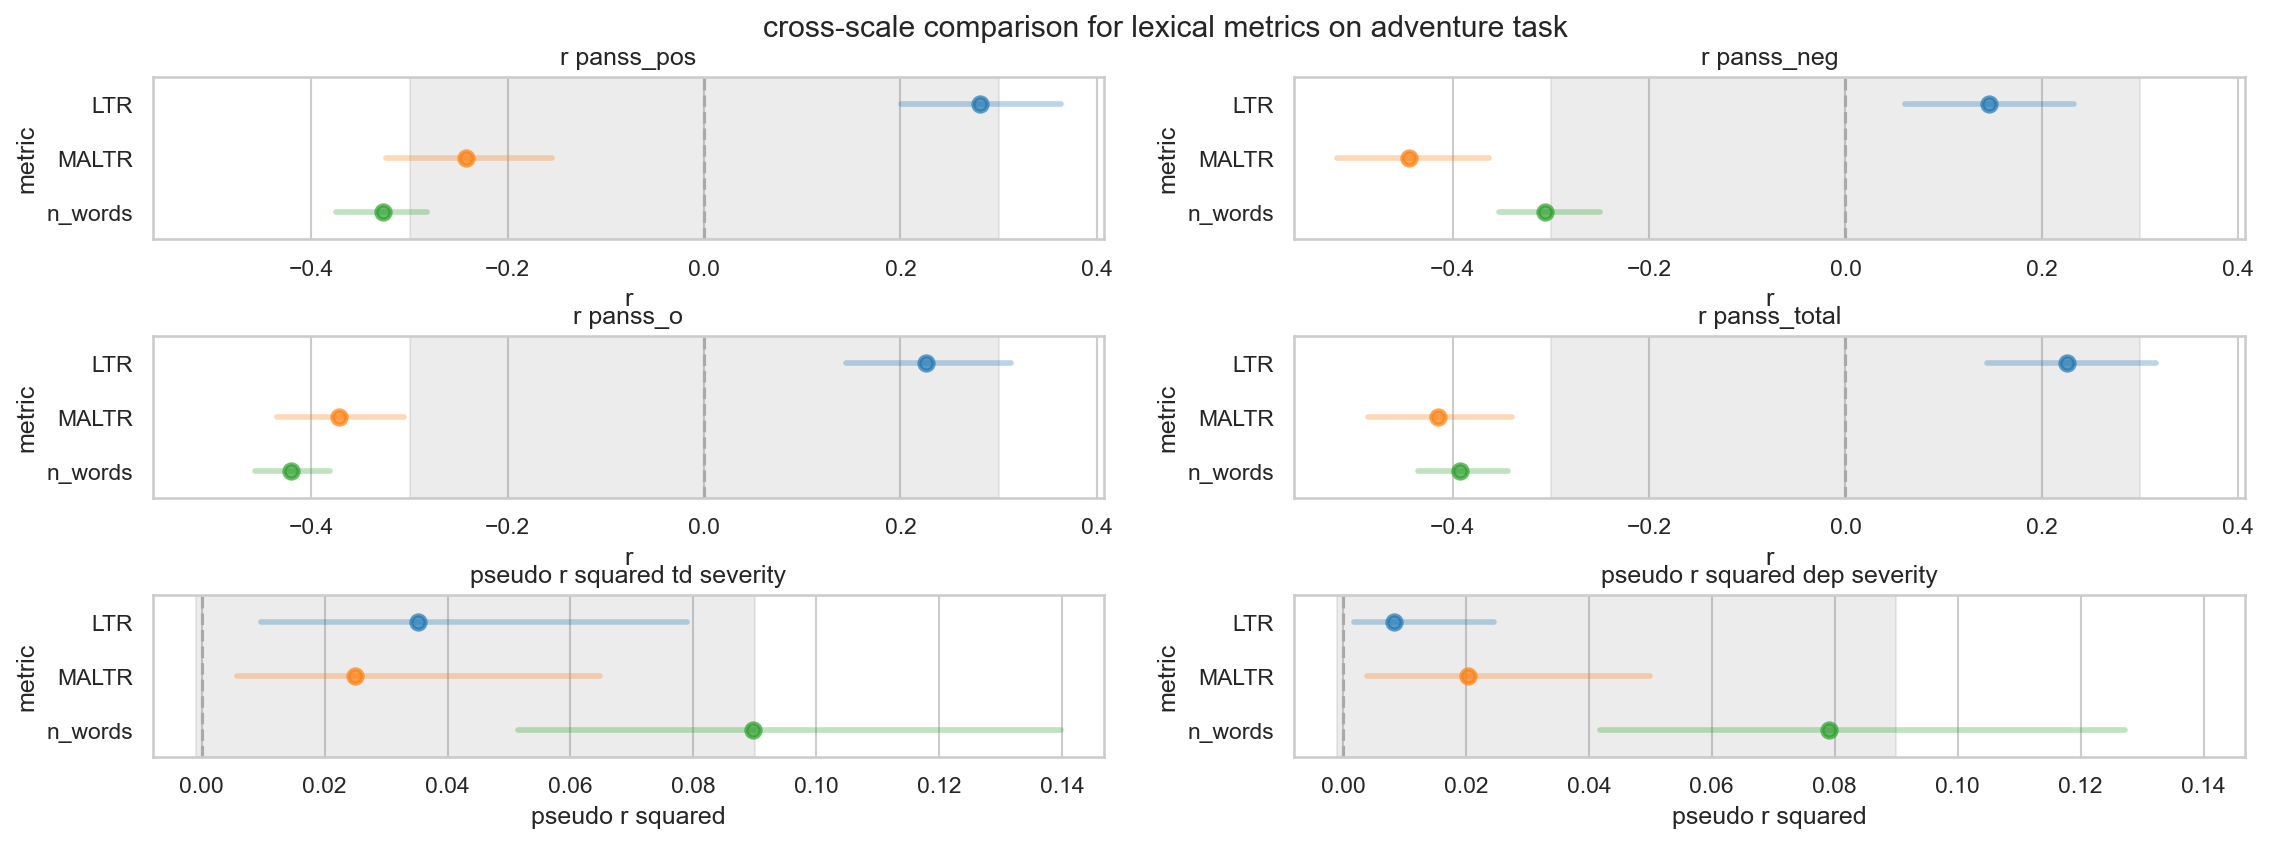
\includegraphics[width=0.9\textwidth, center]{Figures/chapter_4/lexical/ru_adventure_scale_r.png} 
\captionsetup{width=\textwidth}
\caption[Lexical Metrics: Russian, Adventure Task]{\label{fig:results:lexical:ru:ad} Pearson's r correlation coefficient and pseudo r squared for each scale for the lexical metrics on the Russian dataset, adventure task. Grey indicates the values below the 0.3 threshold in absolute value or pseudo r squared below 0.09.}
\end{figure}

On chair task, shown in figure \ref{fig:results:lexical:ch}, LTR correlated positively with all PANSS subscales, and was also predictive of depression severity. Conversely, MALTR and word count both correlated negatively with all PANSS subscales, and word count was also predictive of depression severity on chair task.

\begin{figure}[ht!]
    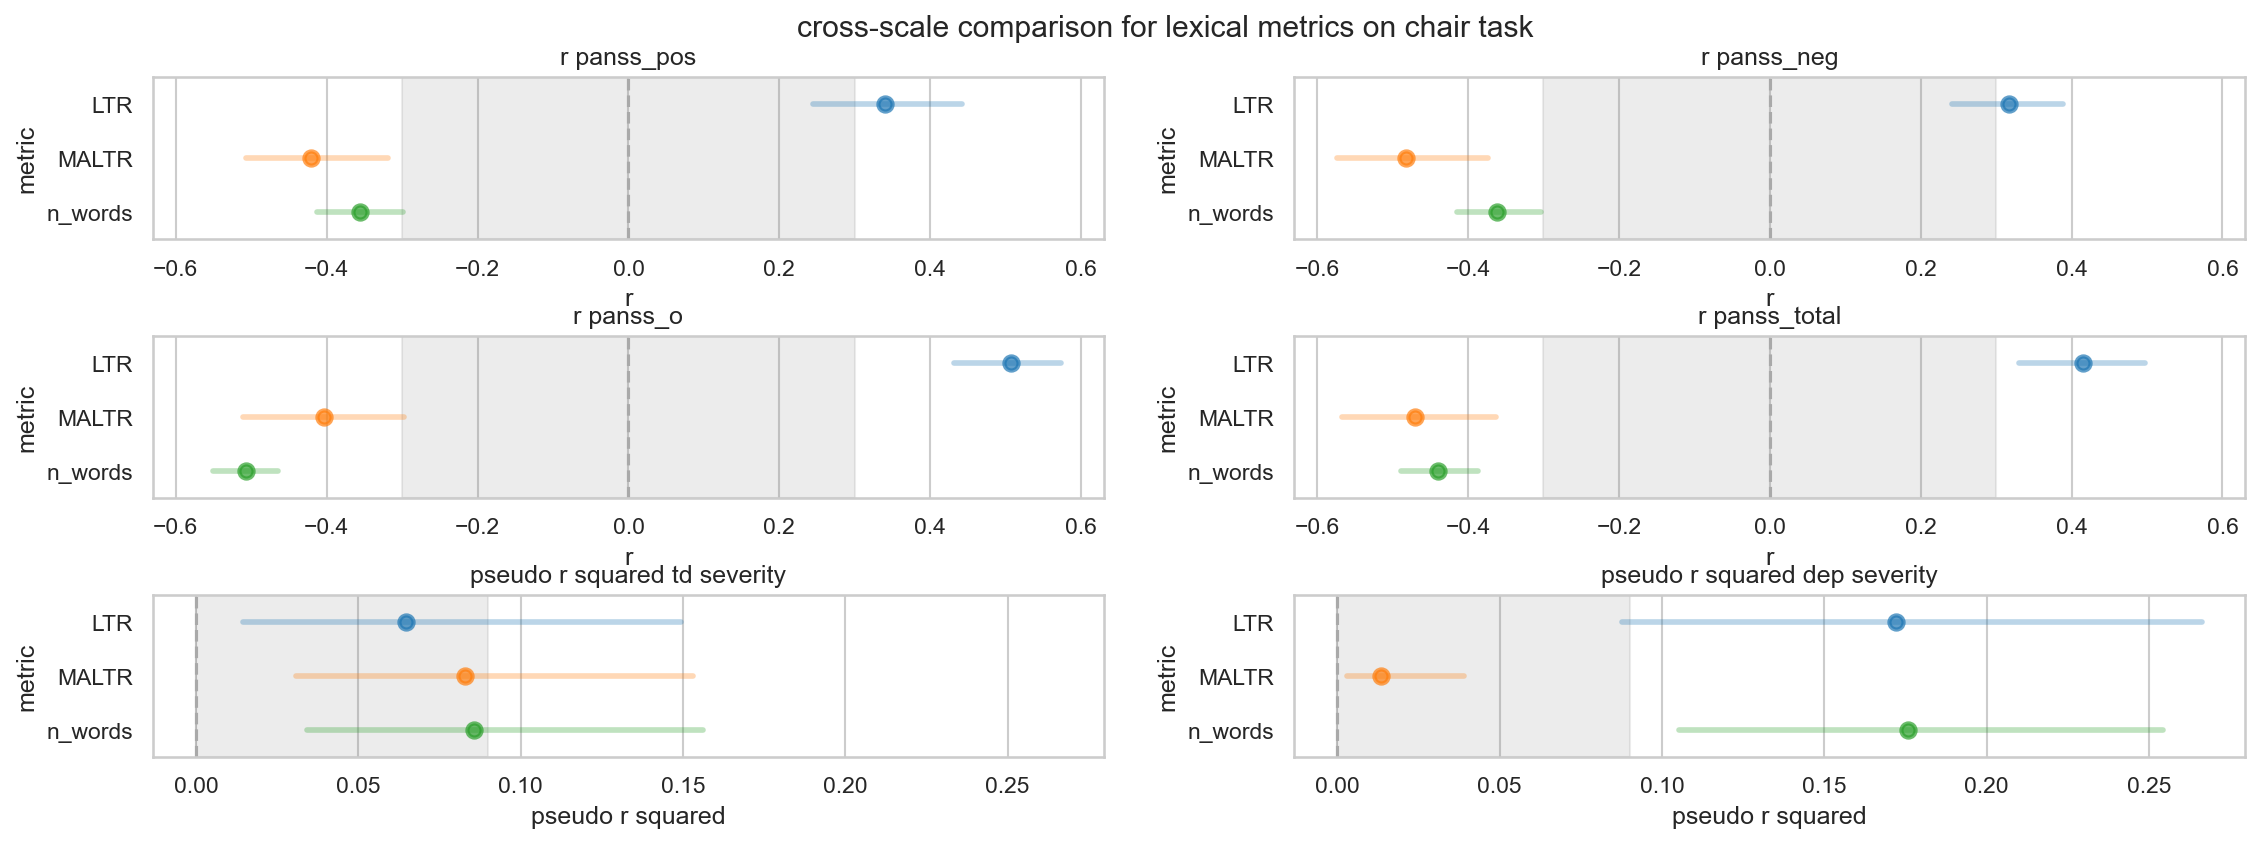
\includegraphics[width=0.9\textwidth, center]{Figures/chapter_4/lexical/ru_chair_scale_r.png} 
\captionsetup{width=\textwidth}
\caption[Lexical Metrics: Russian, Chair Task]{\label{fig:results:lexical:ch} Pearson's r correlation coefficient and pseudo r squared for each scale for the lexical metrics on the Russian dataset, chair task. Grey indicates the values below the 0.3 threshold in absolute value or pseudo r squared below 0.09.}
\end{figure}

On present task, shown in figure \ref{fig:results:lexical:ru:pr}, LTR correlated positively with all PANSS subscales and was predictive of TD severity. MALTR correlated with PANSS negative only, and word count correlated negatively with all PANSS subscales and was also predictive of TD severity.

\begin{figure}[ht!]
    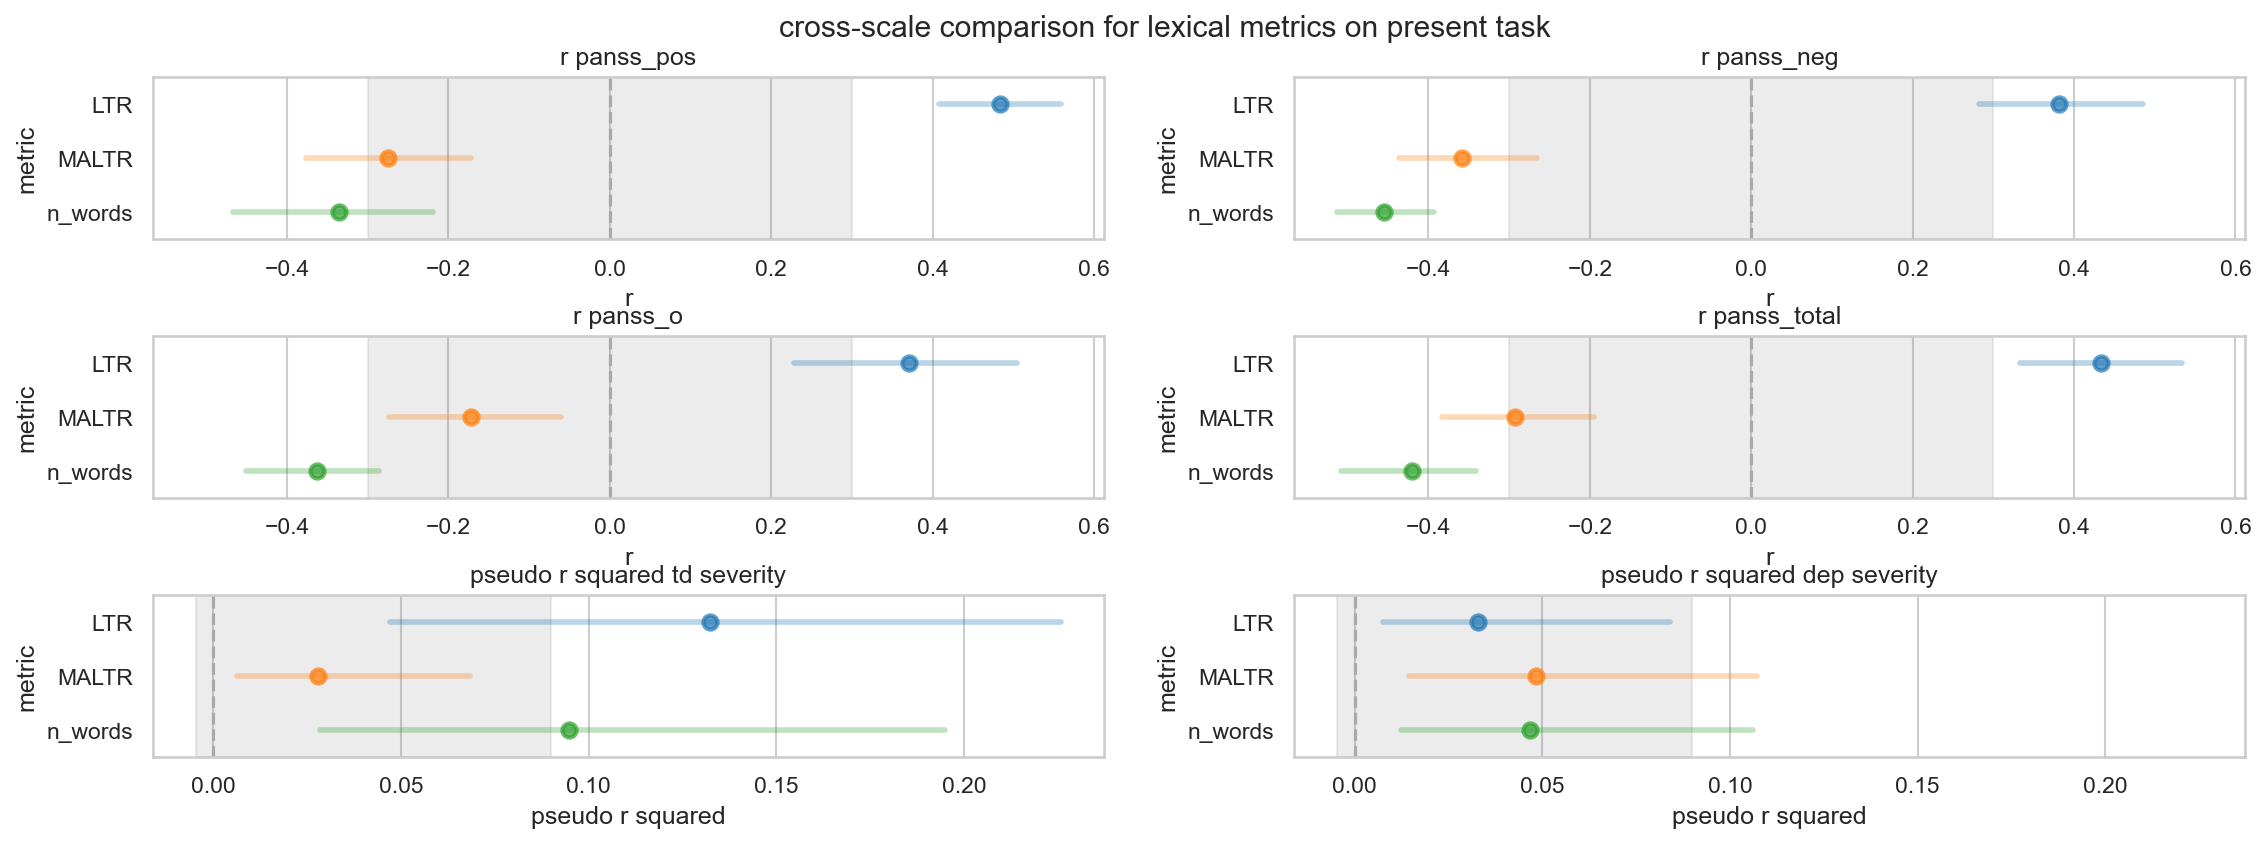
\includegraphics[width=0.9\textwidth, center]{Figures/chapter_4/lexical/ru_present_scale_r.png} 
\captionsetup{width=\textwidth}
\caption[Lexical Metrics: Russian, Present Task]{\label{fig:results:lexical:ru:pr} Pearson's r correlation coefficient and pseudo r squared for each scale for the lexical metrics on the Russian dataset, present task. Grey indicates the values below the 0.3 threshold in absolute value or pseudo r squared below 0.09.}
\end{figure}

Finally, on sportsman task, shown in figure \ref{fig:results:lexical:ru:sp}, LTR also correlated positively with all PANSS subscales and was predictive of TD severity, and word count correlated negatively with all PANSS subscales and was also predictive of TD severity. MALTR did not perform on any of the scales on this task.

\begin{figure}[ht!]
    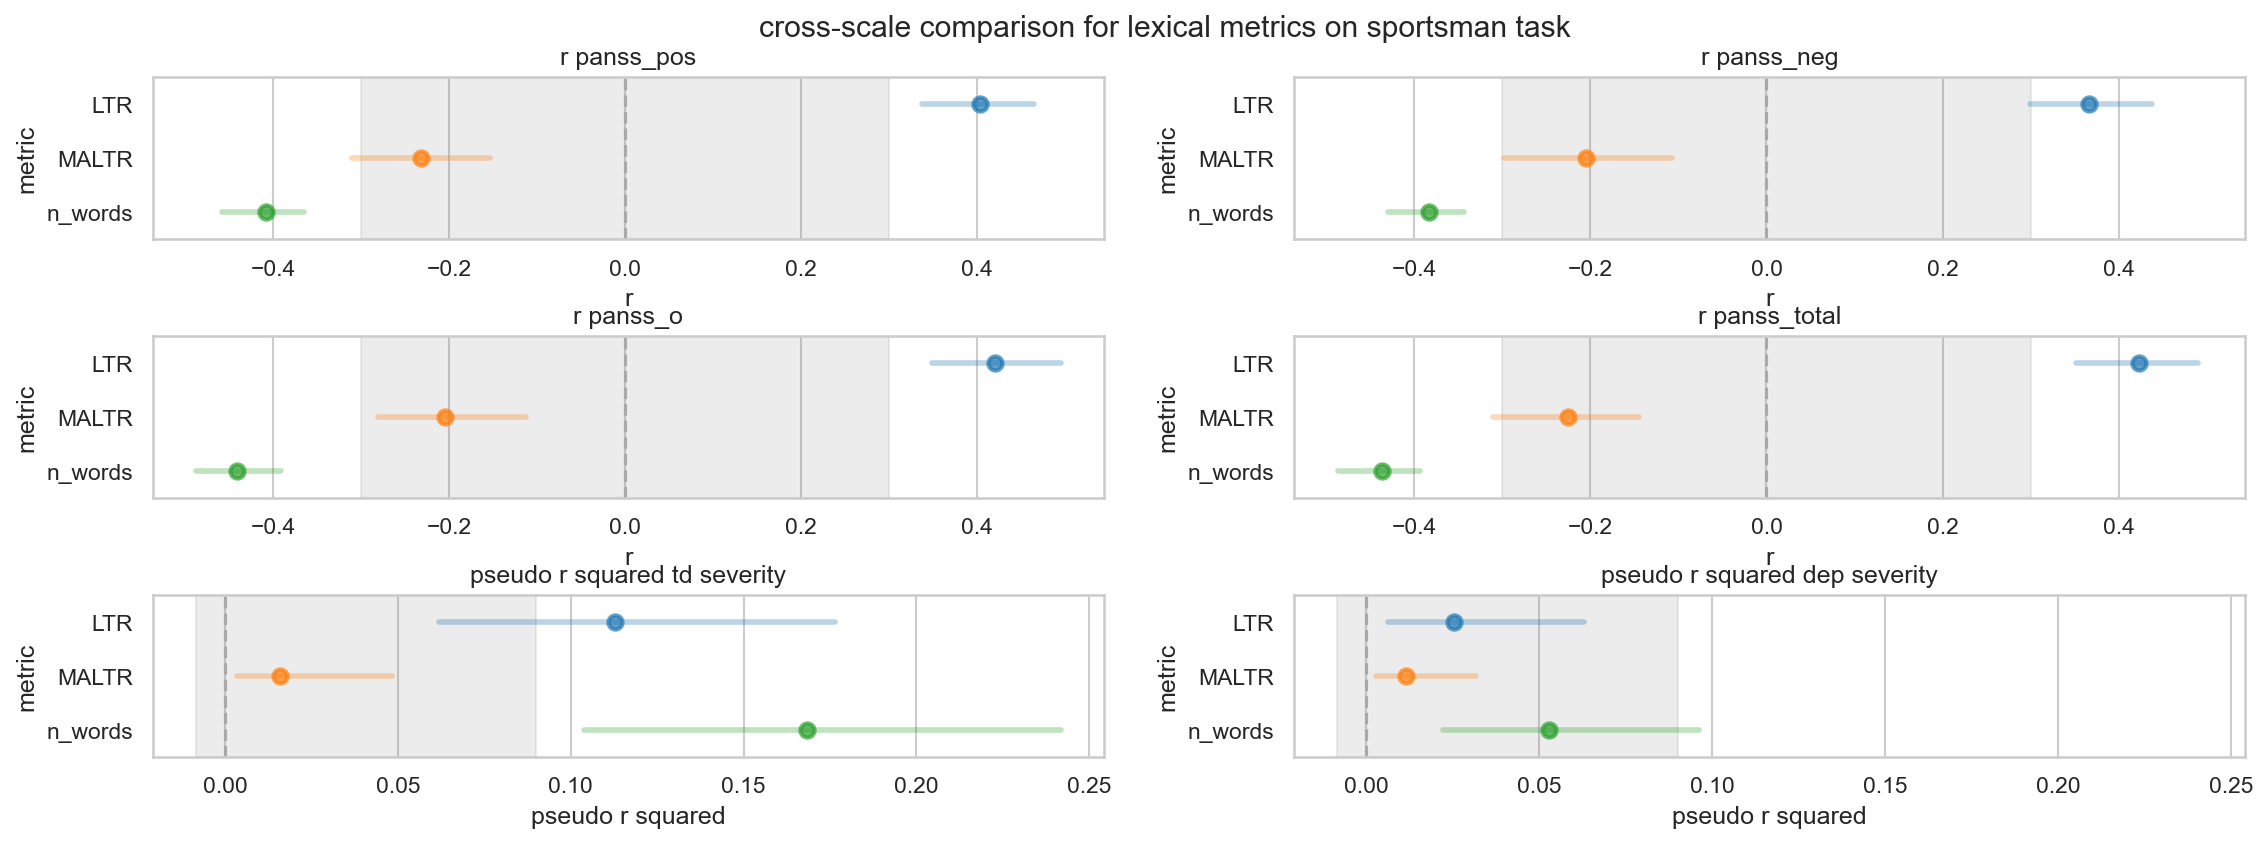
\includegraphics[width=0.9\textwidth, center]{Figures/chapter_4/lexical/ru_sportsman_scale_r.png} 
\captionsetup{width=\textwidth}
\caption[Lexical Metrics: Russian, Sportsman Task]{\label{fig:results:lexical:ru:sp} Pearson's r correlation coefficient and pseudo r squared for each scale for the lexical metrics on the Russian dataset, sportsman task. Grey indicates the values below the 0.3 threshold in absolute value or pseudo r squared below 0.09.}
\end{figure}

Figure \ref{fig:results:lexical:ru:corr_len} shows the strength of correlation with mean sentence length across tasks, indicating that MALTR positively correlated with mean sentence length on all tasks, while word count only does on chair task, and LTR only on sportsman task.

\begin{figure}[ht!]
    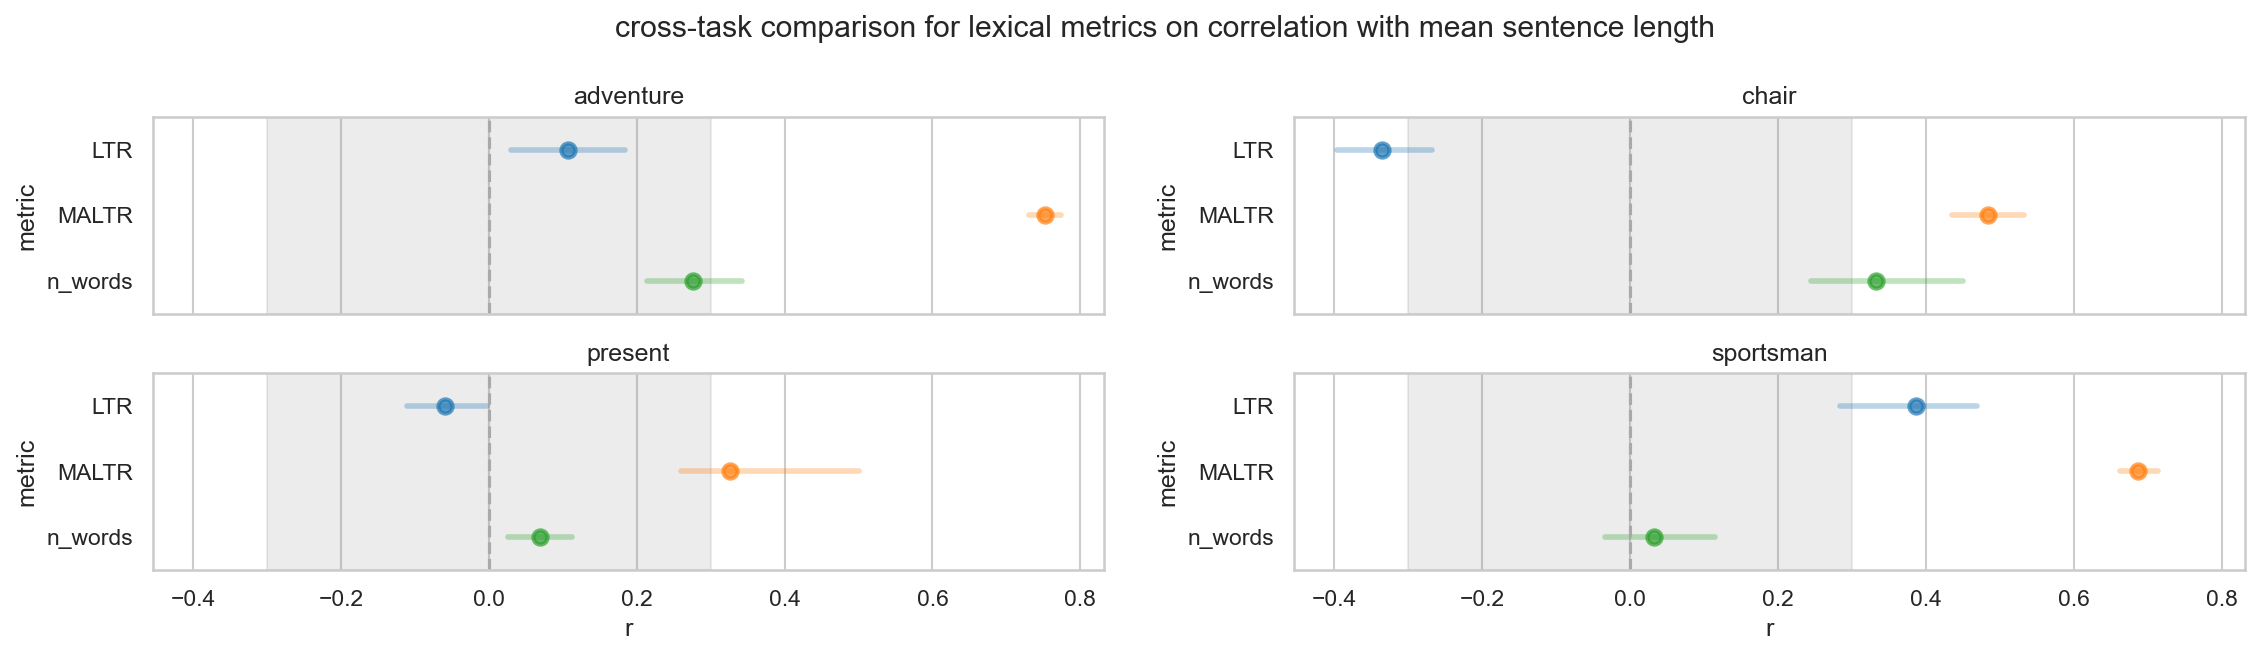
\includegraphics[width=0.9\textwidth, center]{Figures/chapter_4/lexical/ru_corr_len.png} 
\captionsetup{width=\textwidth}
\caption[Lexical Metrics: Russian, Length Correlation]{\label{fig:results:lexical:ru:corr_len} Pearson's r correlation coefficient with mean sentence length for the lexical metrics on the Russian dataset across tasks. Grey indicates the values below 0.3.}
\end{figure}

Overall, on the Russian sample, LTR correlated positively across PANSS subscales but for one task, and word count correlated negatively across PANSS subscales but for one task, while MALTR only performed on two tasks. LTR and word count were also predictive of TD severity on two tasks and of depression severity on one task, while not being overly strongly correlated with mean sentence length.

\subsection{Cross-Linguistic Comparison}
The direction of the correlation for the lexical metrics, was similar between the languages, while the strength of correlation as well as the correlation with mean sentence length differed across scales, tasks, and languages. 


%-----------------------------------
%	section 5
%-----------------------------------
\clearpage
\section{Syntactic Methods}
\label{sec:results:clinical:syntactic}
This section covers the performance of syntactic metrics, including mean, maximal, and minimal sentence length, along with standard deviation in sentence length (mean\_, min\_, max\_, and std\_  sent\_len, respectively), and total sentence count (n sents). Part-of-speech (POS) rates are also tested for the parts-of-speech that were shown to perform in some of the literature, namely: adjectives (ADJ), adverbs (ADV), auxiliary verbs (AUX), coordinating and subordinating conjunctions (CCONJ, SCONJ), determiners (DET), nouns and proper nouns (NOUN, PRPON), pronouns (PRON), particles (PART), and verbs (VERB).

\subsection{German}
The performance of the syntactic metrics on the German sample is shown in figure \ref{fig:results:syntactic:de}. 

\begin{figure}[h!]
    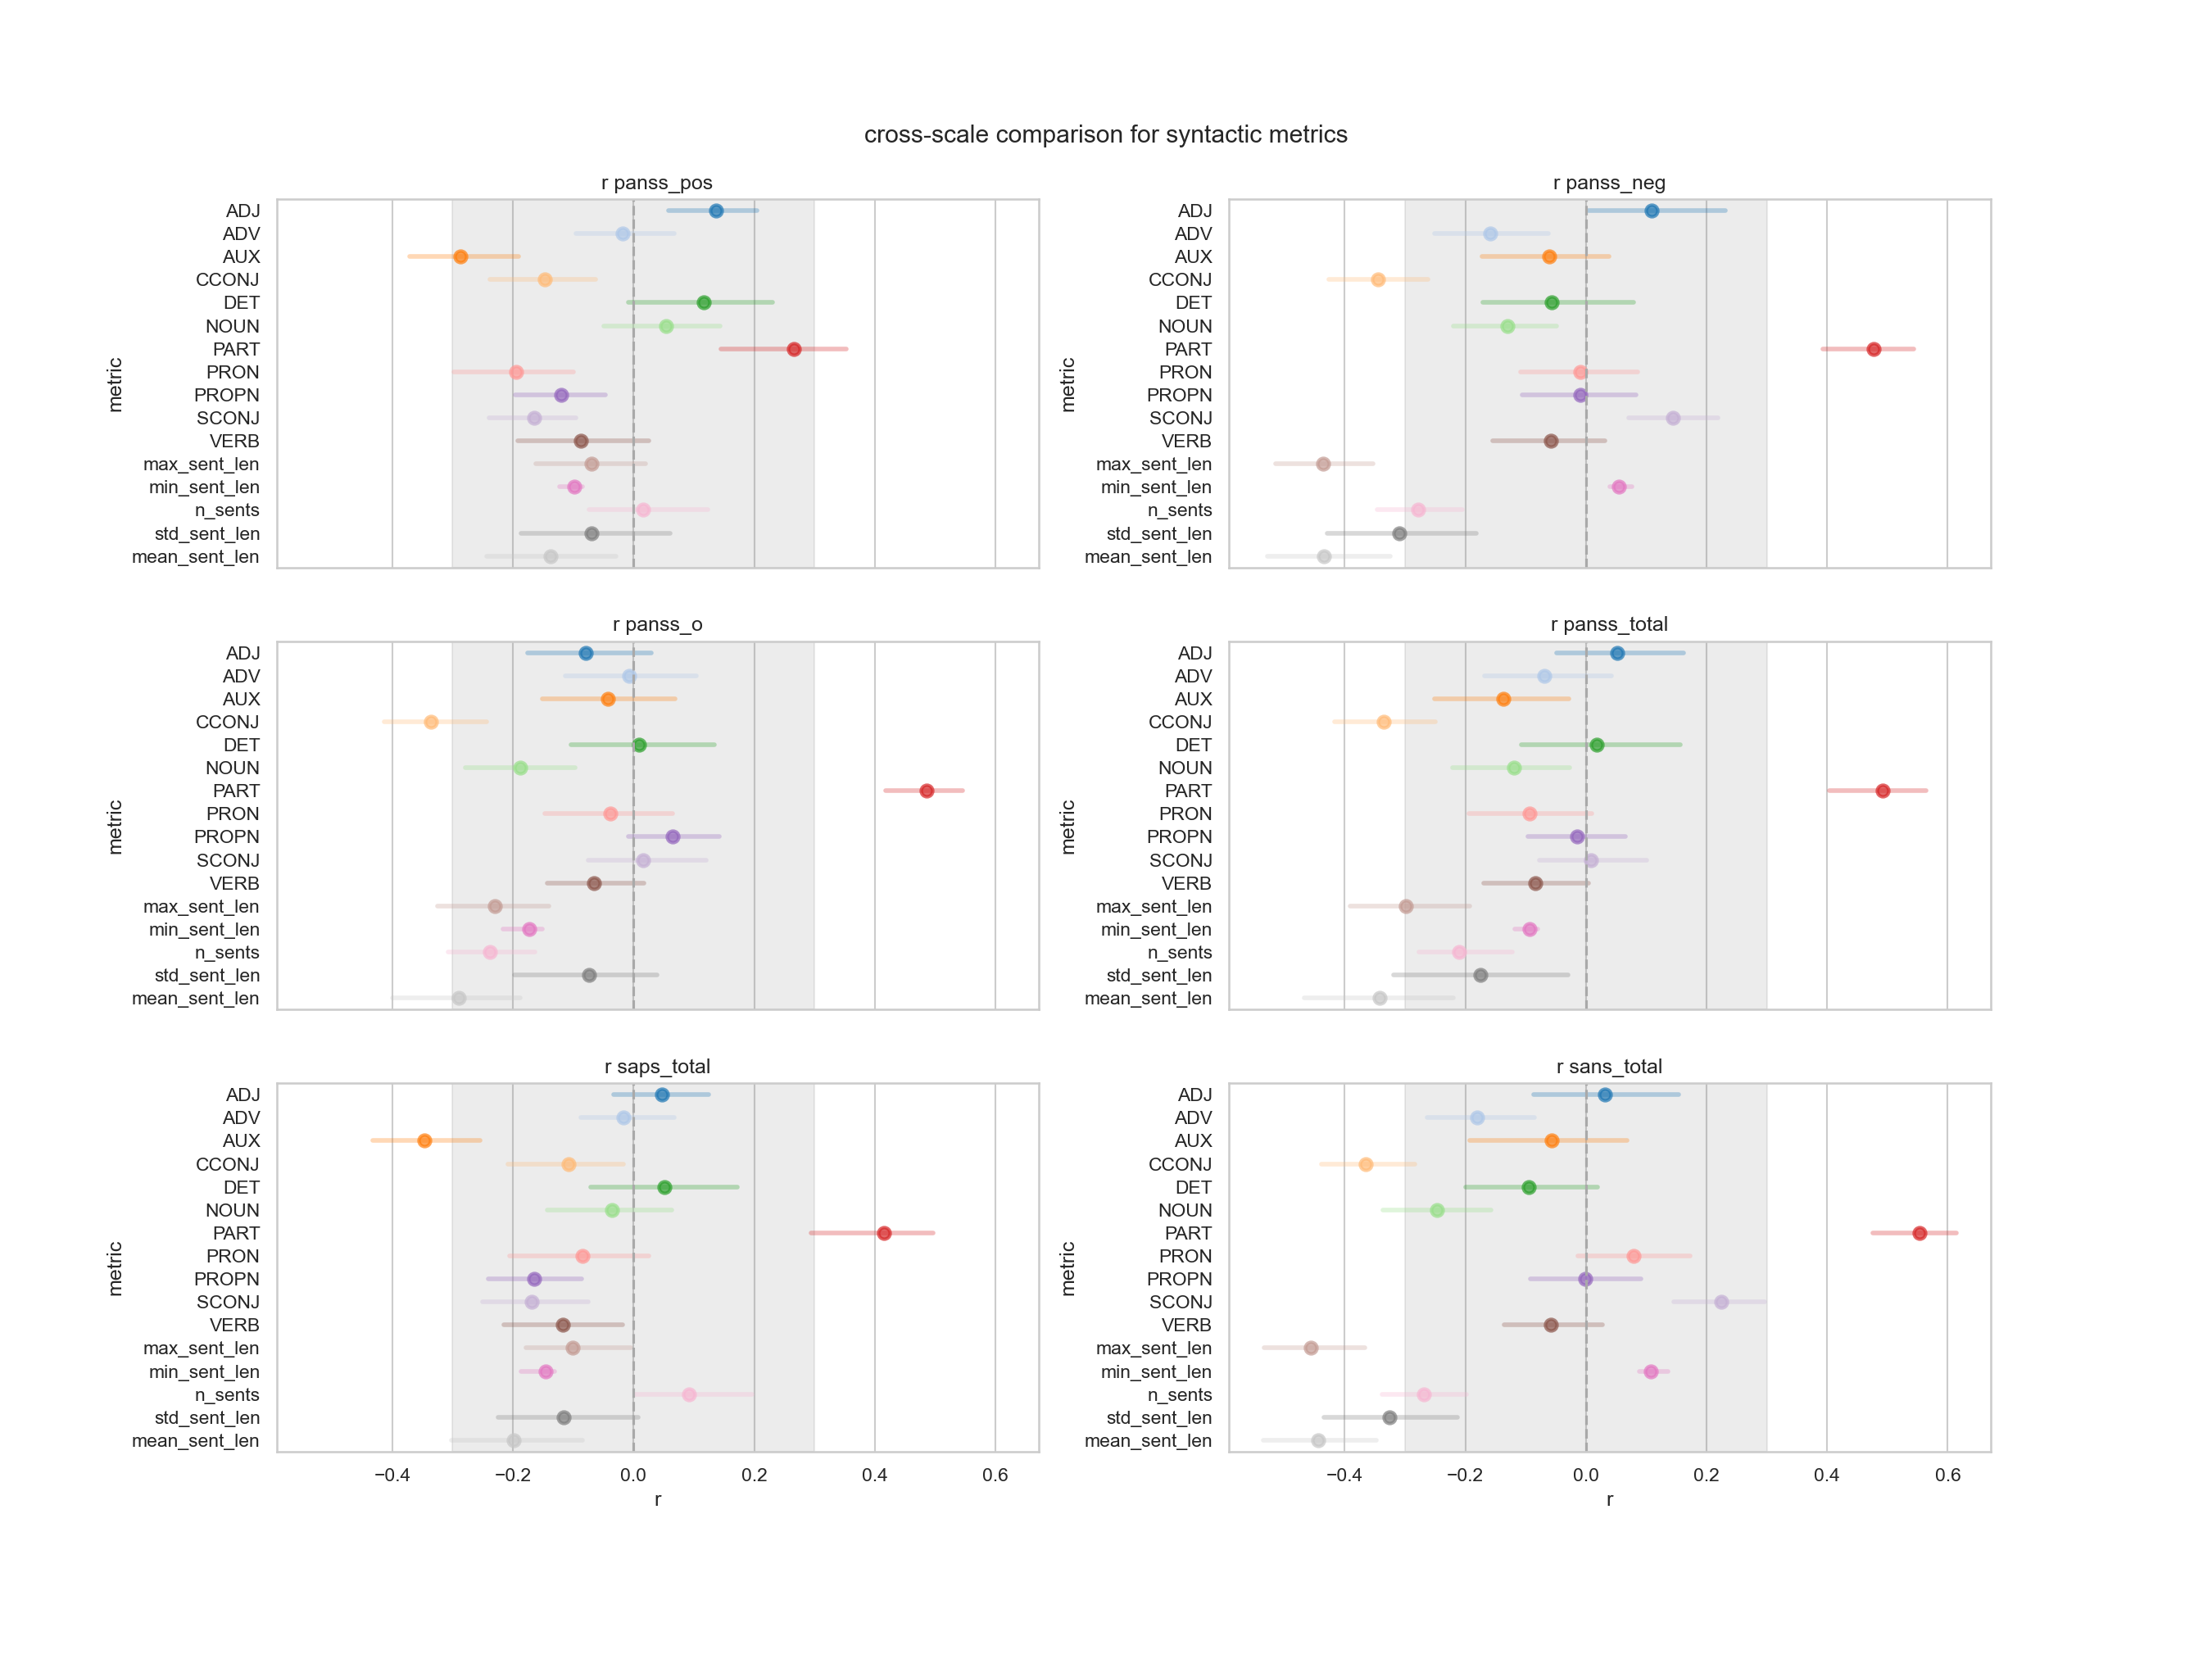
\includegraphics[width=1.2\textwidth, center]{Figures/chapter_4/syntactic/de_scale_r.png} 
\captionsetup{width=\textwidth}
\caption[Syntactic Metrics: German]{\label{fig:results:syntactic:de} Pearson's r correlation coefficient with each scale for the syntactic metrics on the German dataset. Grey indicates the values below the 0.3 threshold in absolute value.}
\end{figure}

Among the POS rate metrics, only PART, AUX, and CCONJ correlated consistently with any of the scales. PART use correlated positively with all scales, but PANSS positive. AUX correlated negatively with all scales, but the positive ones, while CCONJ correlated negatively only with SAPS total score. As for the other syntactic metrics, maximum, mean, and minimal sentence length showed the best performance, as they correlated negatively with all negative scales as well as with PANSS total score, except for minimal sentence length. None of the other metrics correlated with any of the scales.

\clearpage
\begin{figure}[ht!]
    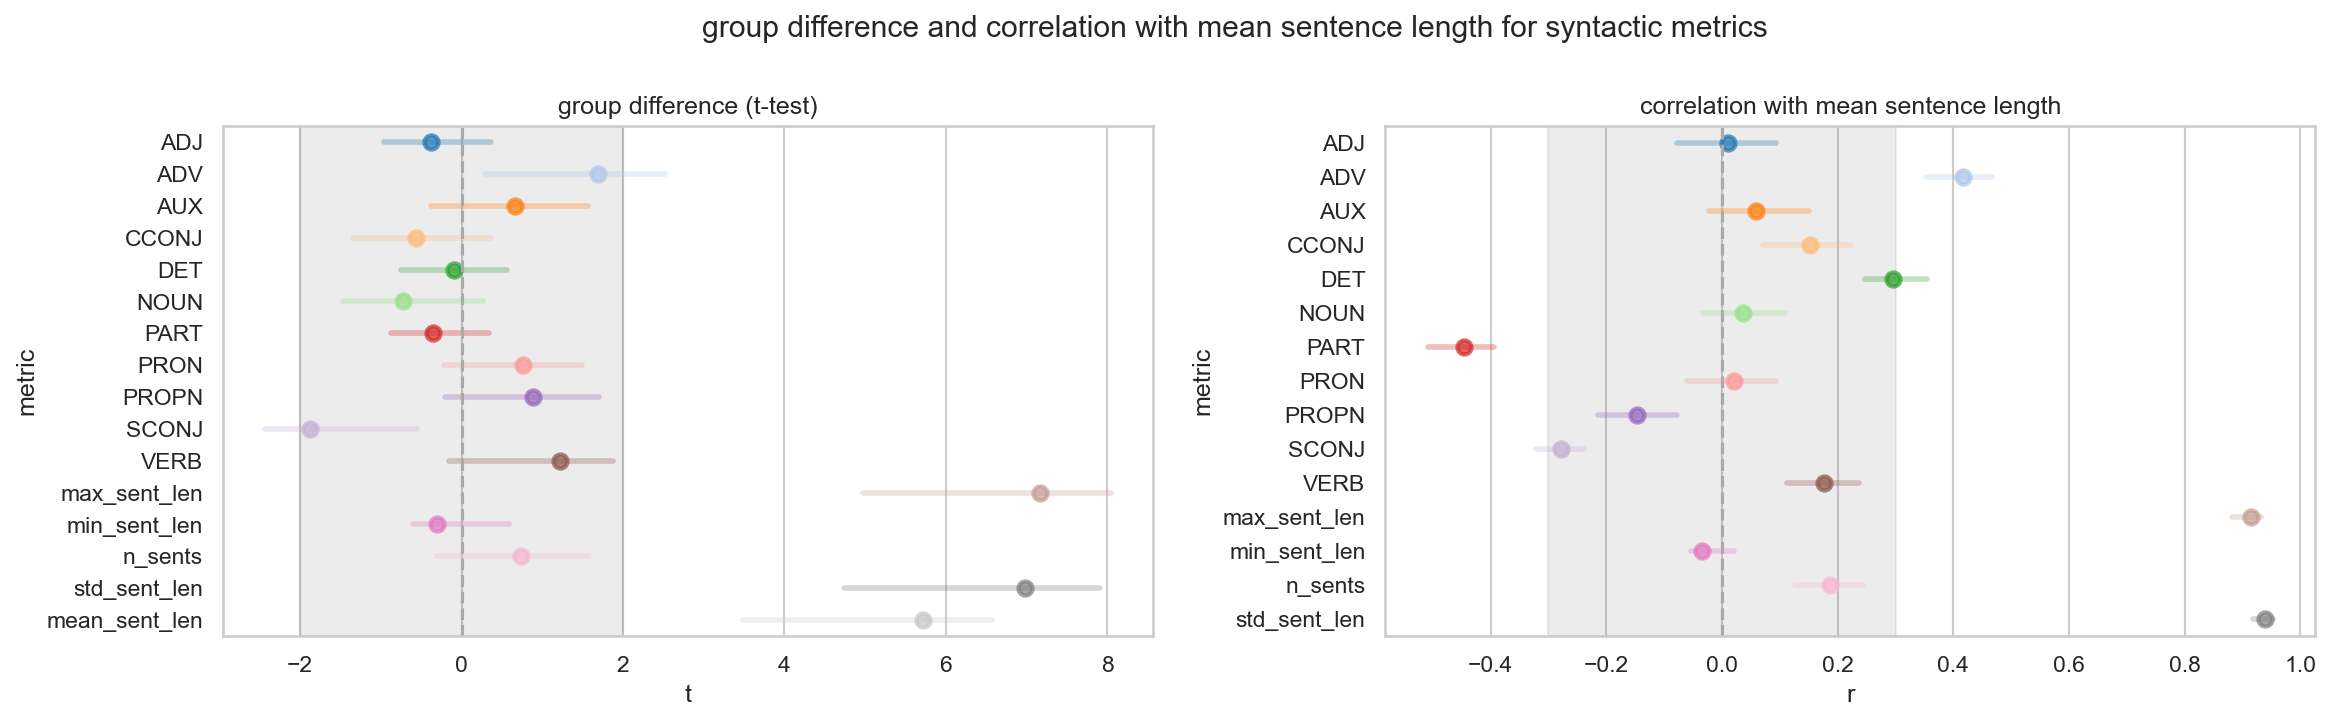
\includegraphics[width=1.1\textwidth, center]{Figures/chapter_4/syntactic/de_t_test_corr_len.png} 
\captionsetup{width=\textwidth}
\caption[Syntactic Metrics: German (T-Test)]{\label{fig:results:syntactic:de:ttest} T-test and Pearson's r correlation coefficient with mean sentence length for the syntactic metrics on the German dataset. Grey indicates the values below 2 for t score and below the 0.3 threshold in absolute value for correlation coefficient.}
\end{figure}


Figure \ref{fig:results:syntactic:de:ttest} compares the strength of the t-test to the corresponding correlation with mean sentence length. Mean sentence length is a reasonable baseline for the German sample, and both maximal and minimal sentence length, as could be expected, correlated strongly with it, somewhat outperforming it on the t-test. PART correlated negatively with mean sentence length, while ADV correlated positively with it.

\clearpage
\subsection{Russian}

Figure \ref{fig:results:syntactic:ru:ad} shows the performance of the syntactic metrics on the adventure task, and the only metric that correlated with any of the symptom scales is the total number of sentences, which correlated negatively with general symptoms and total PANSS score.

\begin{figure}[ht!]
    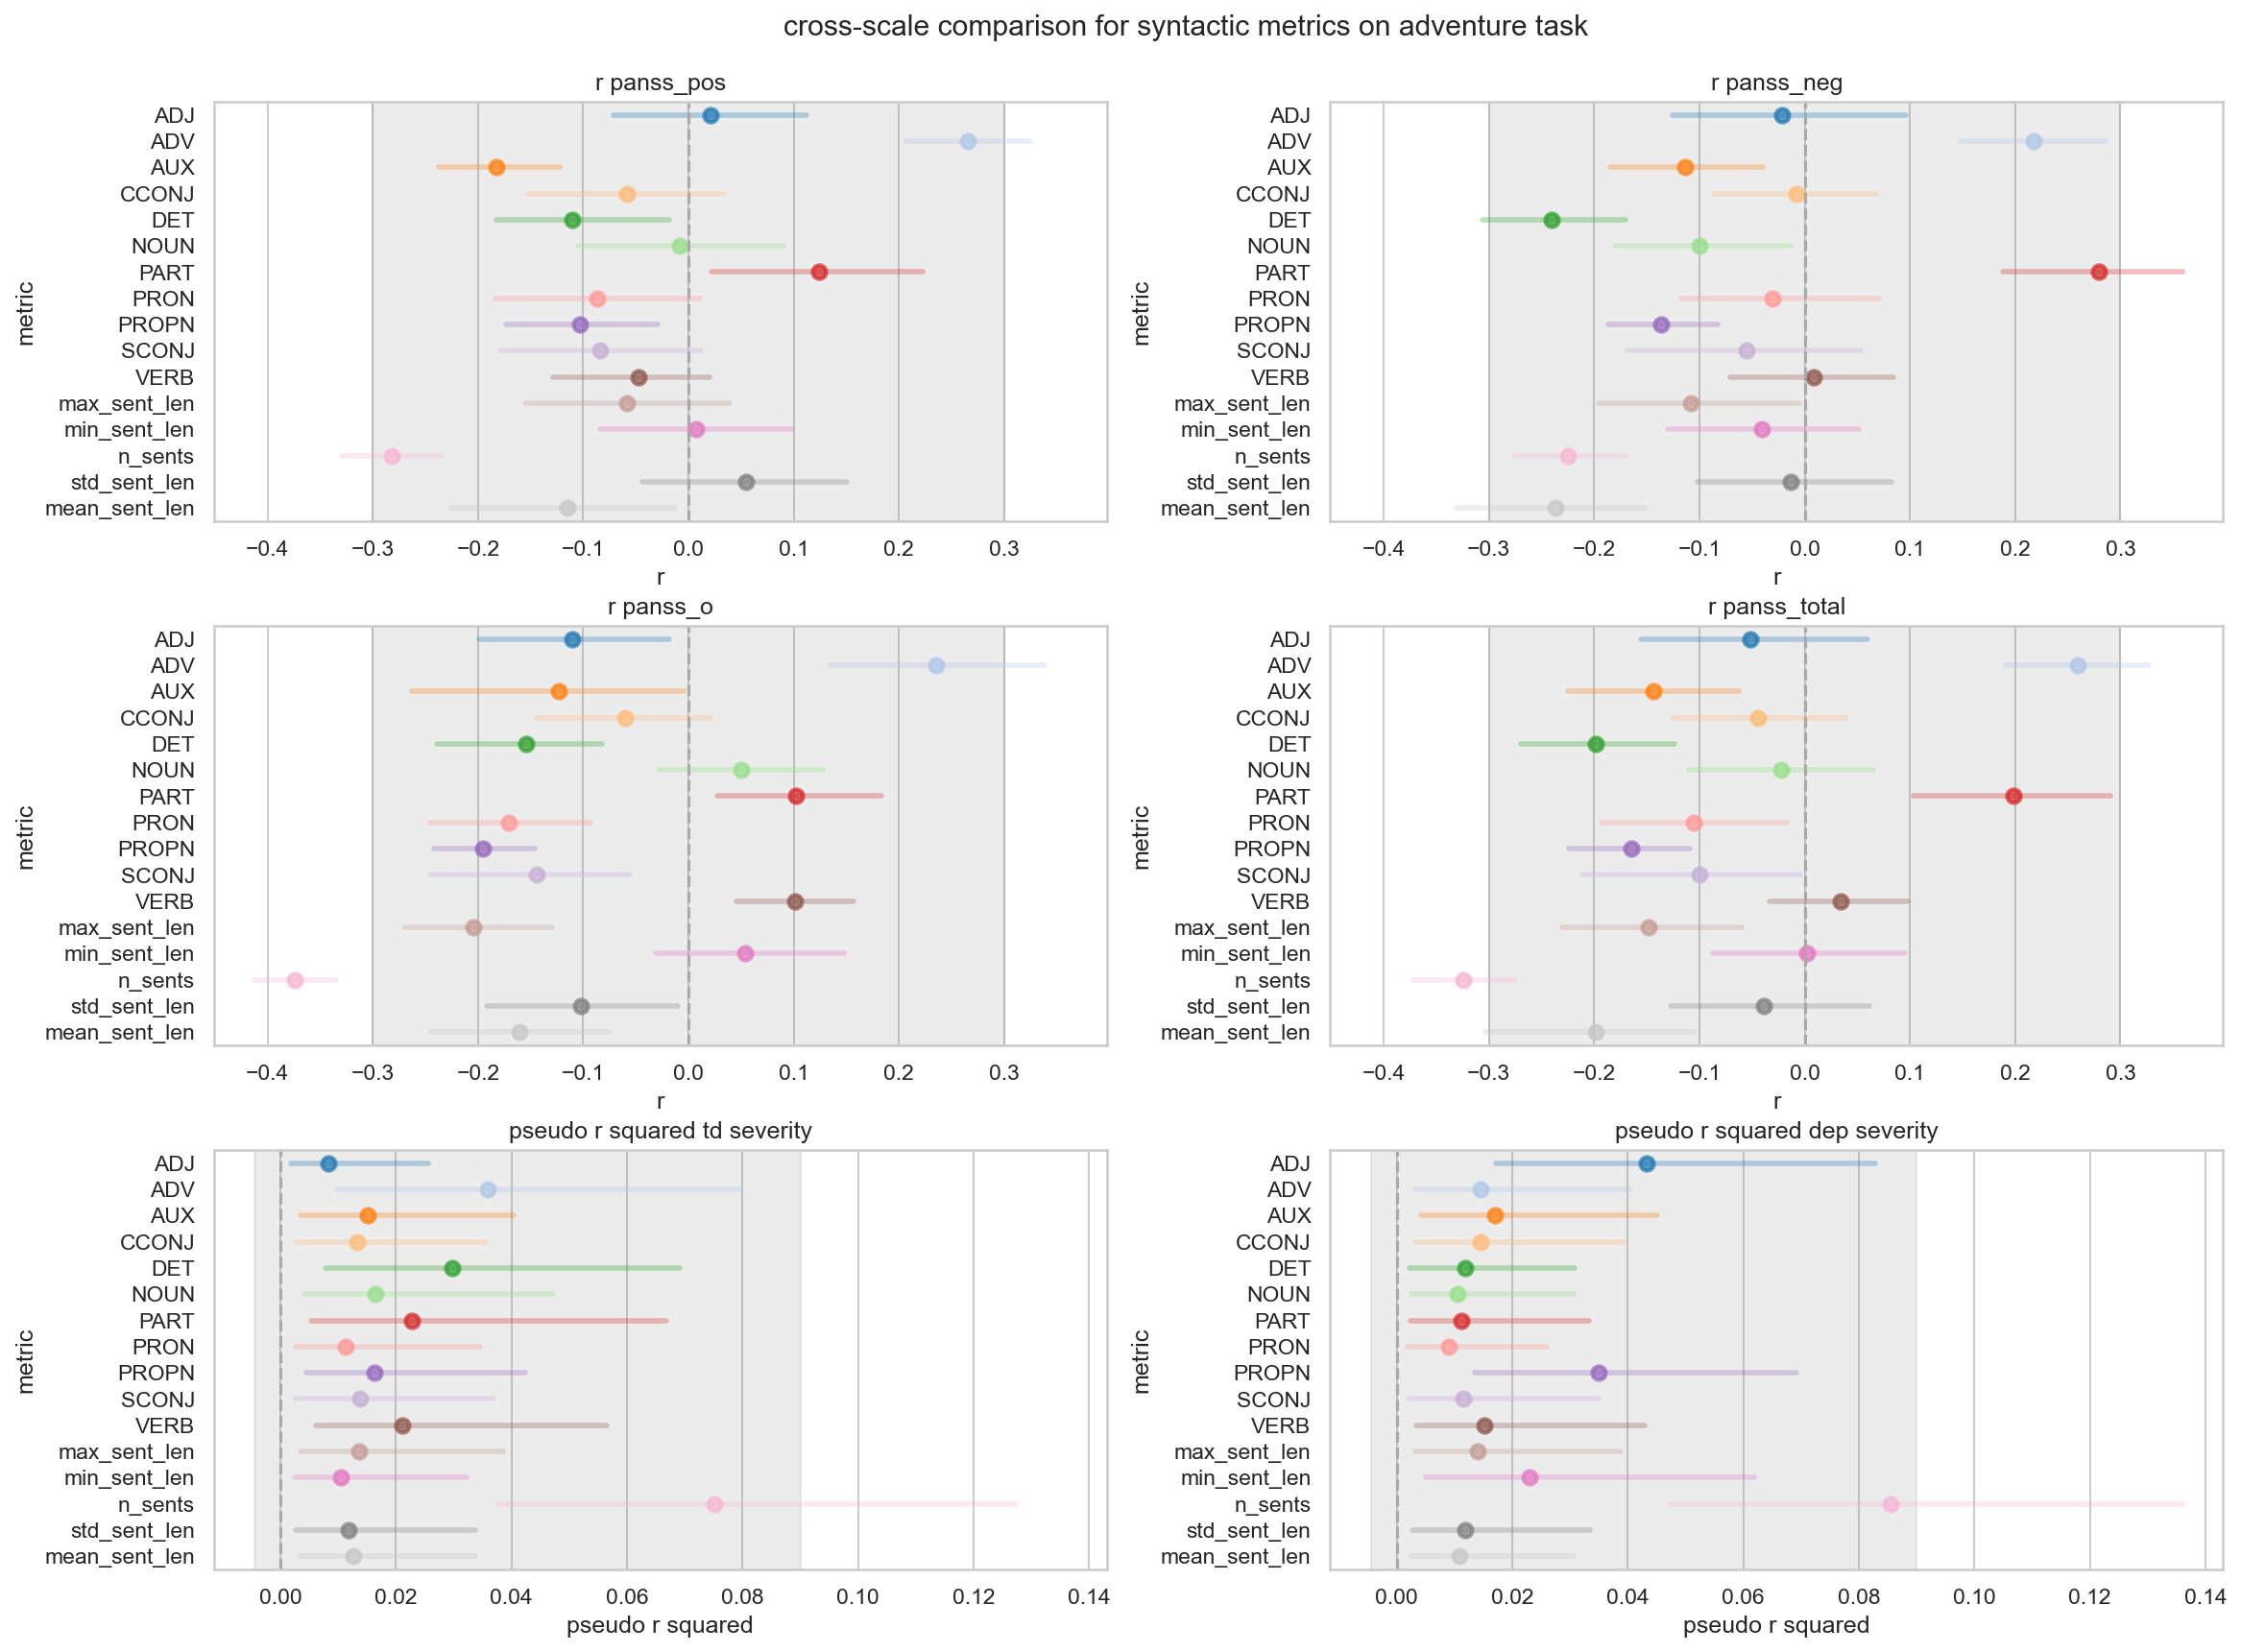
\includegraphics[width=1.1\textwidth, center]{Figures/chapter_4/syntactic/ru_adventure_scale_r.png} 
\captionsetup{width=\textwidth}
\caption[Syntactic Metrics: Russian, Adventure Task]{\label{fig:results:syntactic:ru:ad} Pearson's r correlation coefficient and pseudo r squared for each scale for the syntactic metrics on the Russian dataset, adventure task. Grey indicates the values below the 0.3 threshold in absolute value or pseudo r squared below 0.09.}
\end{figure}

\clearpage
Figure \ref{fig:results:syntactic:ru:ch} shows the performance of the syntactic metrics on the chair task. Among the parts of speech, PART rate correlated with all PANSS subscales, and NOUN rate with all but the general symptoms subscale. These two metrics were also the only ones performing well in TD severity detection. The mean sentence length correlated with all PANSS subscales as well as predicted depression severity along with maximal sentence length. The total number of sentences correlated with all PANSS subscales but PANSS negative.

\begin{figure}[ht!]
    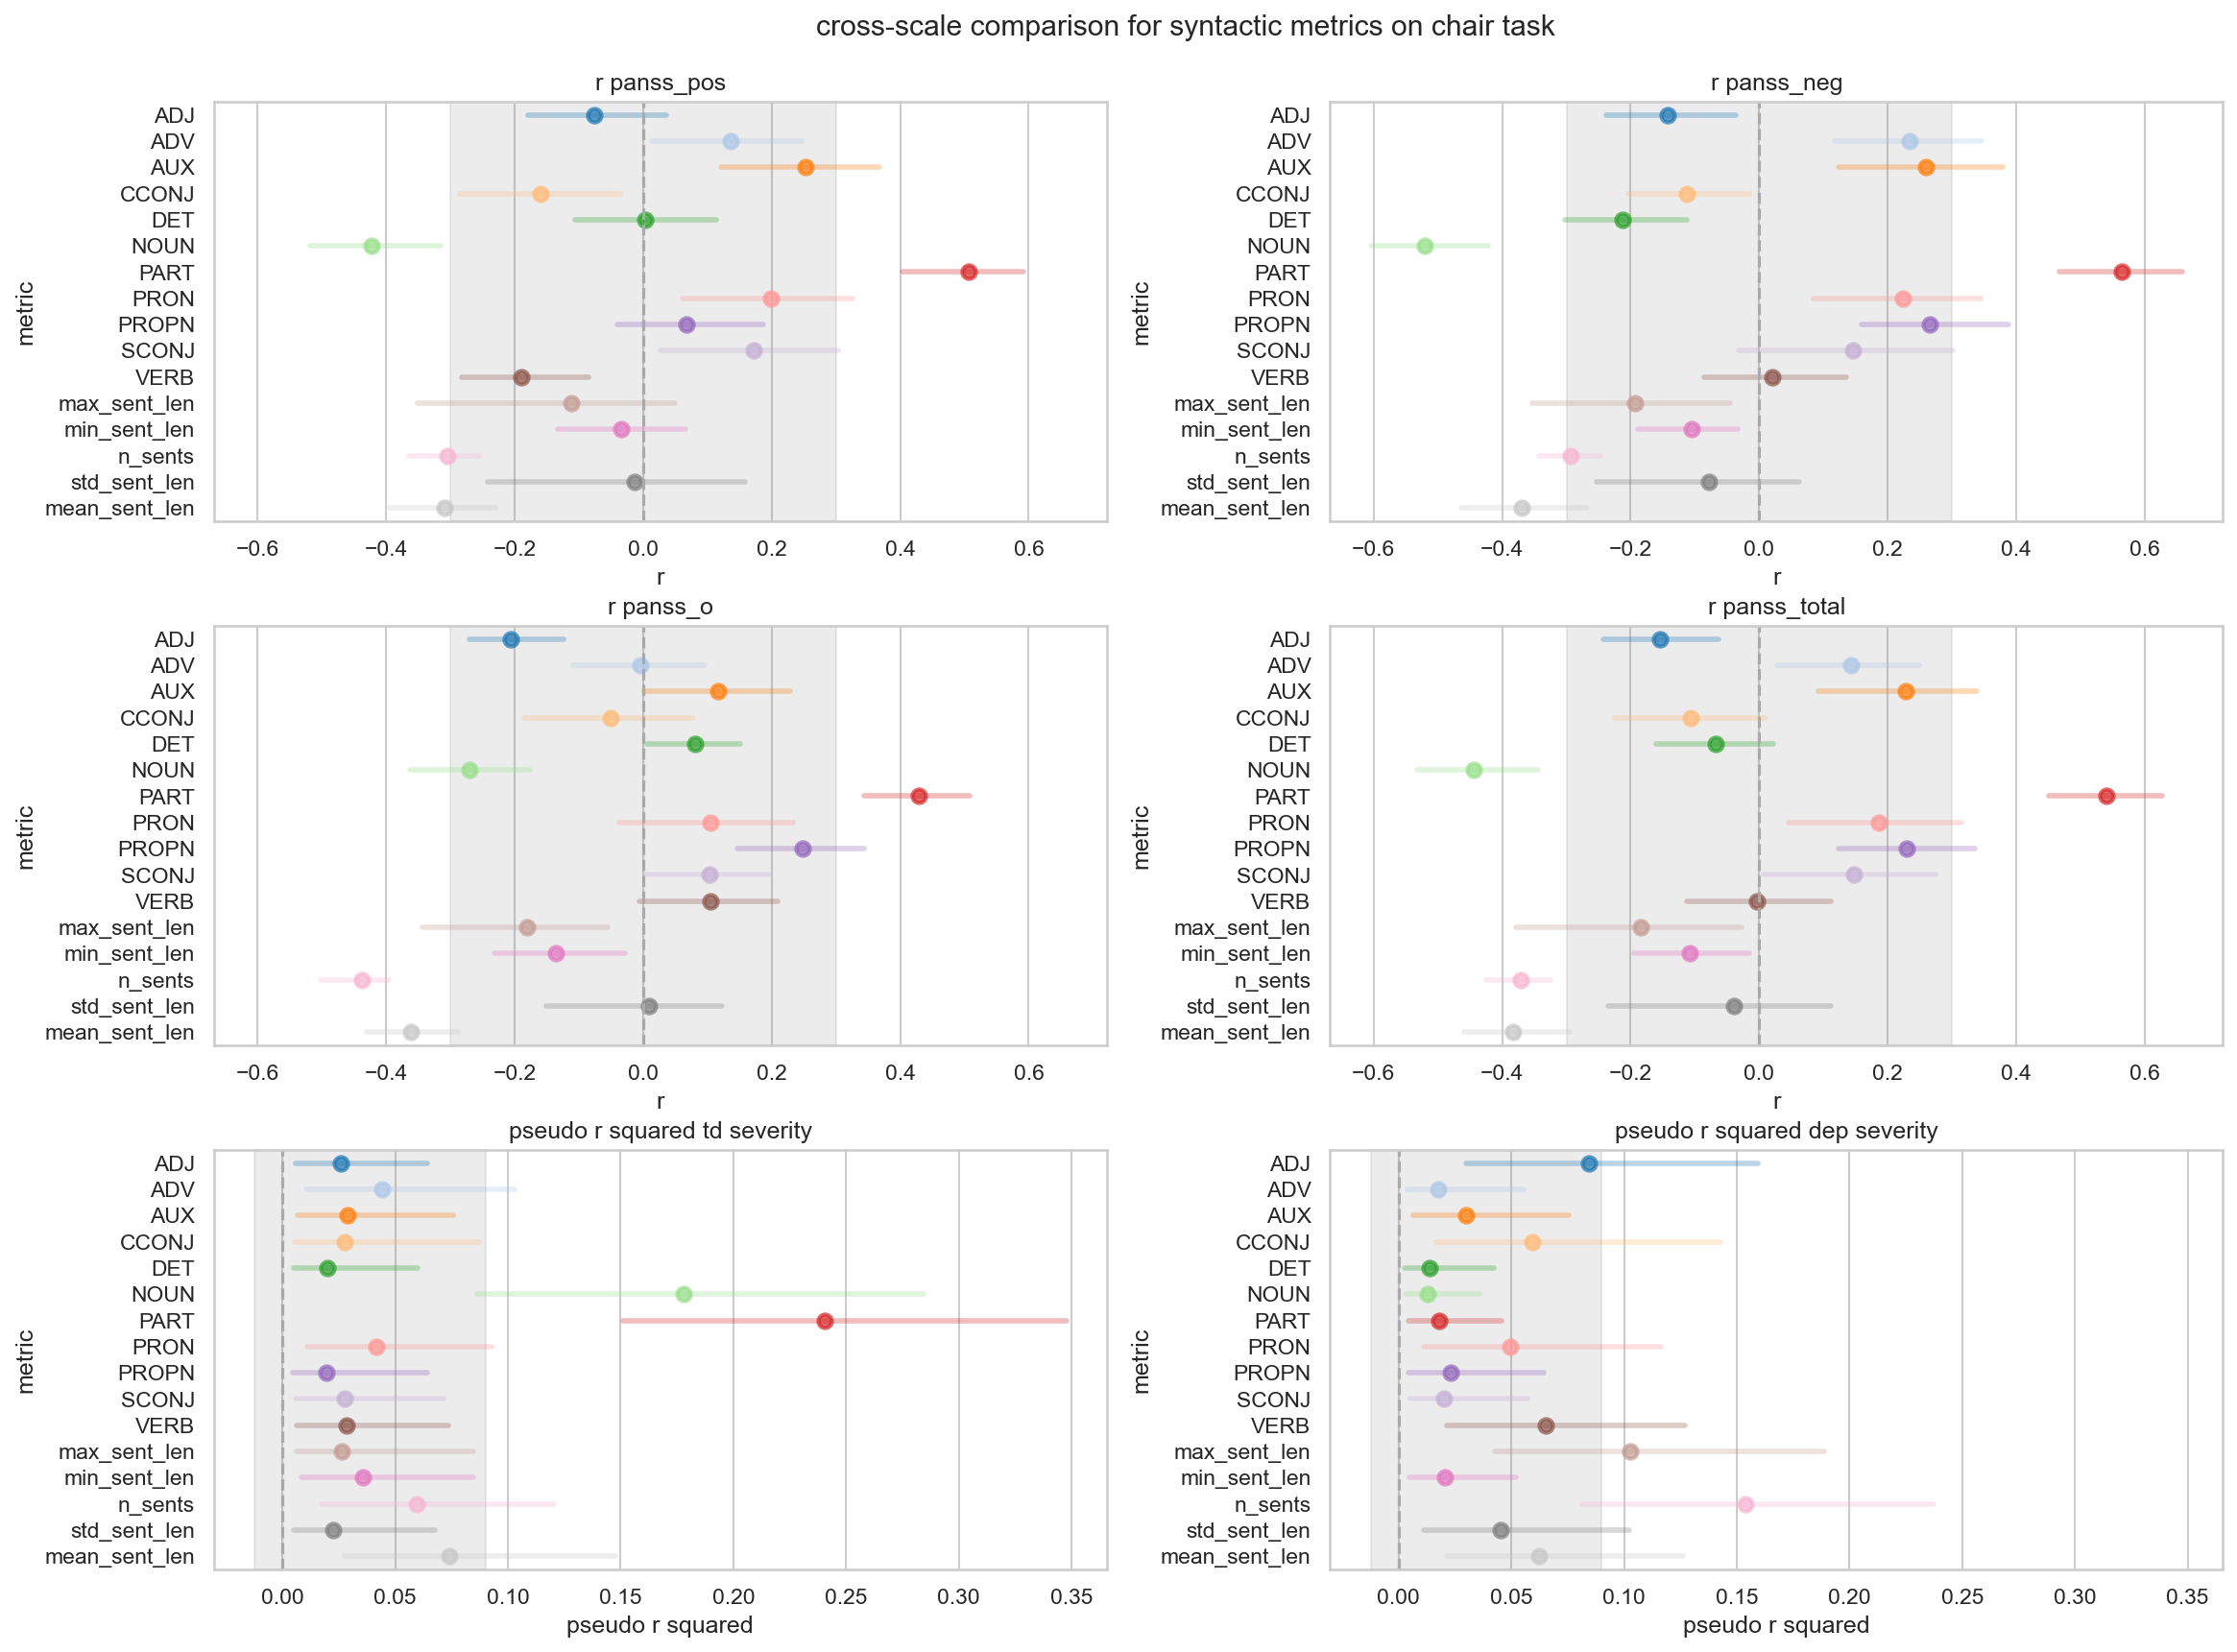
\includegraphics[width=1.1\textwidth, center]{Figures/chapter_4/syntactic/ru_chair_scale_r.png} 
\captionsetup{width=\textwidth}
\caption[Syntactic Metrics: Russian, Chair Task]{\label{fig:results:syntactic:ru:ch} Pearson's r correlation coefficient and pseudo r squared for each scale for the syntactic metrics on the Russian dataset, chair task. Grey indicates the values below the 0.3 threshold in absolute value or pseudo r squared below 0.09.}
\end{figure}

\clearpage
Figure \ref{fig:results:syntactic:ru:pr} shows the performance of the syntactic metrics on the present task. PART rate correlated positively with PANSS positive and total scores, DET rate correlated negatively with PANSS negative and total scores, and CCONJ rate correlated negatively with PANSS general only. The total number of sentences correlated negatively with PANSS negative only, while mean sentence length did so with all PANSS scales but the positive. Maximal sentence length and the standard deviation correlated negatively with all PANSS scales and also performed well in TD severity detection, largely outperforming mean sentence length.

\begin{figure}[ht!]
    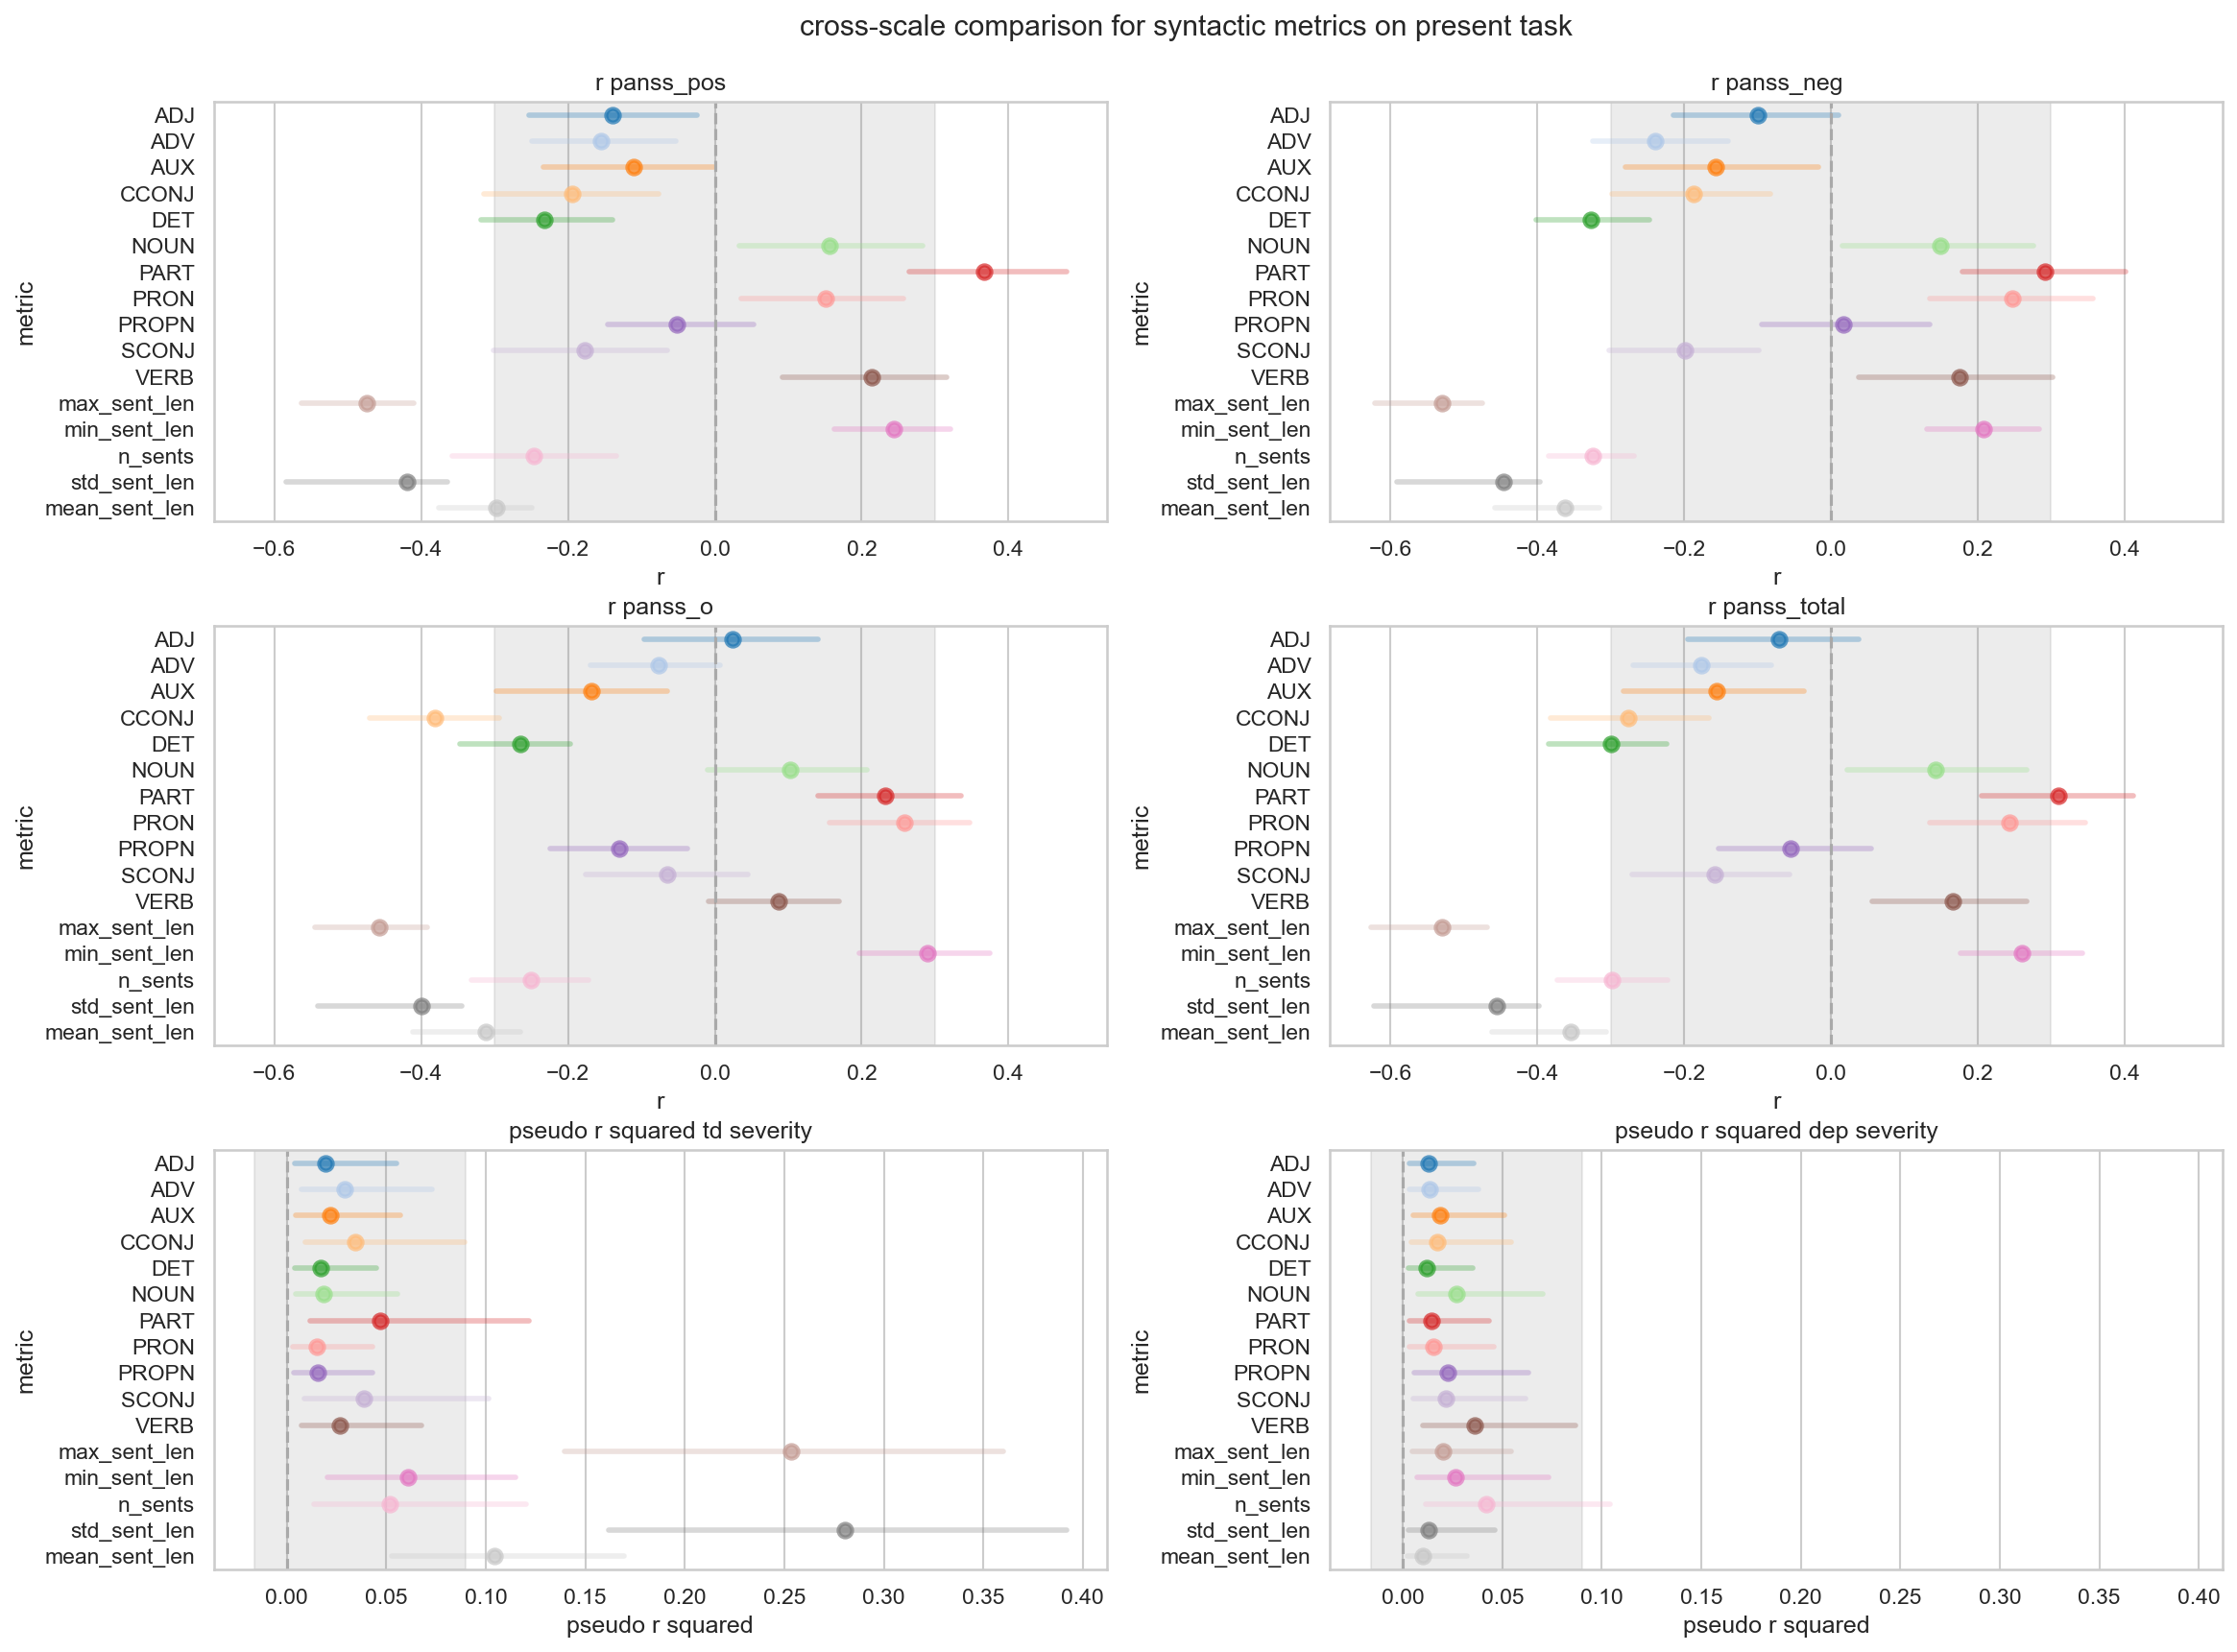
\includegraphics[width=1.1\textwidth, center]{Figures/chapter_4/syntactic/ru_present_scale_r.png} 
\caption[Syntactic Metrics: Russian, Present Task]{\label{fig:results:syntactic:ru:pr} Pearson's r correlation coefficient and pseudo r squared for each scale for the syntactic metrics on the Russian dataset, present task. Grey indicates the values below the 0.3 threshold in absolute value or pseudo r squared below 0.09.}
\end{figure}

\clearpage
Figure \ref{fig:results:syntactic:ru:sp} shows the performance of the syntactic metrics on the sportsman task. On this task, PART correlated positively only with PANSS positive, while maximal sentence length correlated with it negatively. The number of sentences on the other hand correlated negatively with all PANSS scales and was also the only metric sensitive to TD severity.

\begin{figure}[ht!]
    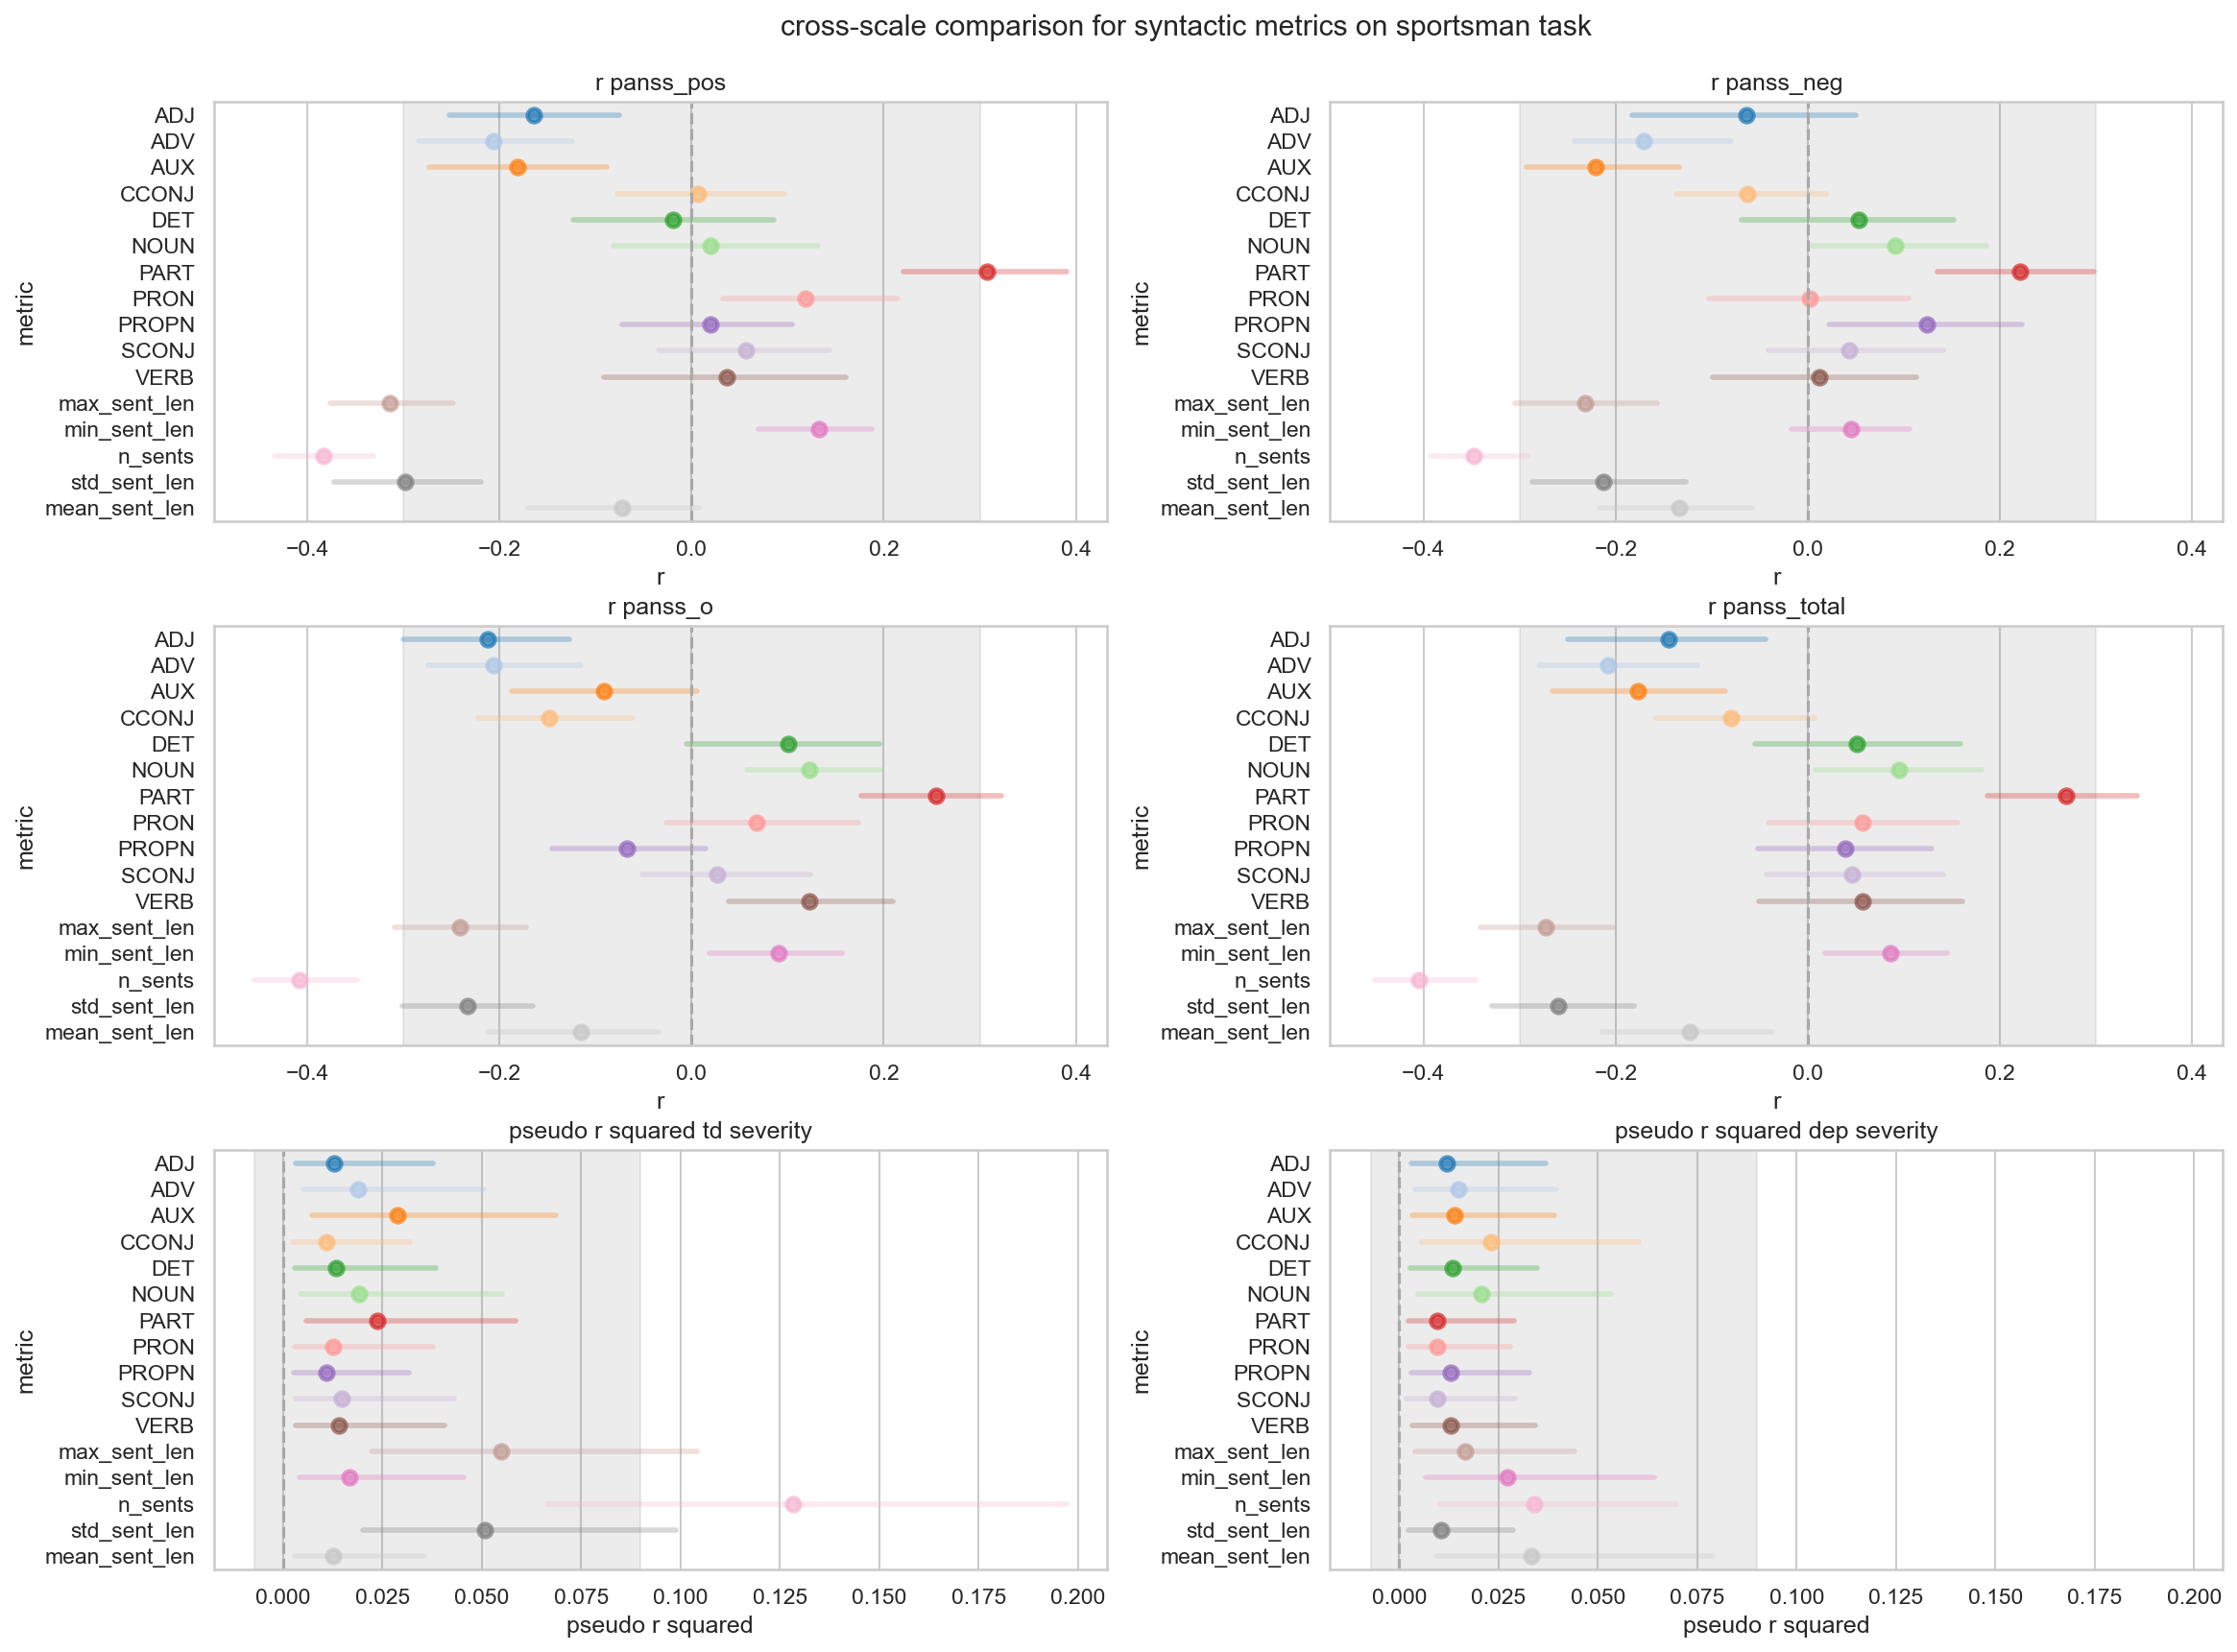
\includegraphics[width=1.1\textwidth, center]{Figures/chapter_4/syntactic/ru_sportsman_scale_r.png} 
\captionsetup{width=\textwidth}
\caption[Syntactic Metrics: Russian, Sportsman Task]{\label{fig:results:syntactic:ru:sp} Pearson's r correlation coefficient and pseudo r squared for each scale for the syntactic metrics on the Russian dataset, sportsman task. Grey indicates the values below the 0.3 threshold in absolute value or pseudo r squared below 0.09.}
\end{figure}

\clearpage
Figure \ref{fig:results:syntactic:ru:corr_len} shows the strength of correlation with mean sentence length across tasks. As could be expected, on all tasks, maximal, standard deviation, and minimal sentence length correlated positively with the mean. VERB rate correlated negatively with mean sentence length on sportsman and adventure tasks, and ADV did so on chair task, while ADJ correlated positively with mean sentence length on all tasks present, and NOUN did so on chair task. Importantly, it is on the chair task that NOUN performed well. 

\begin{figure}[ht!]
    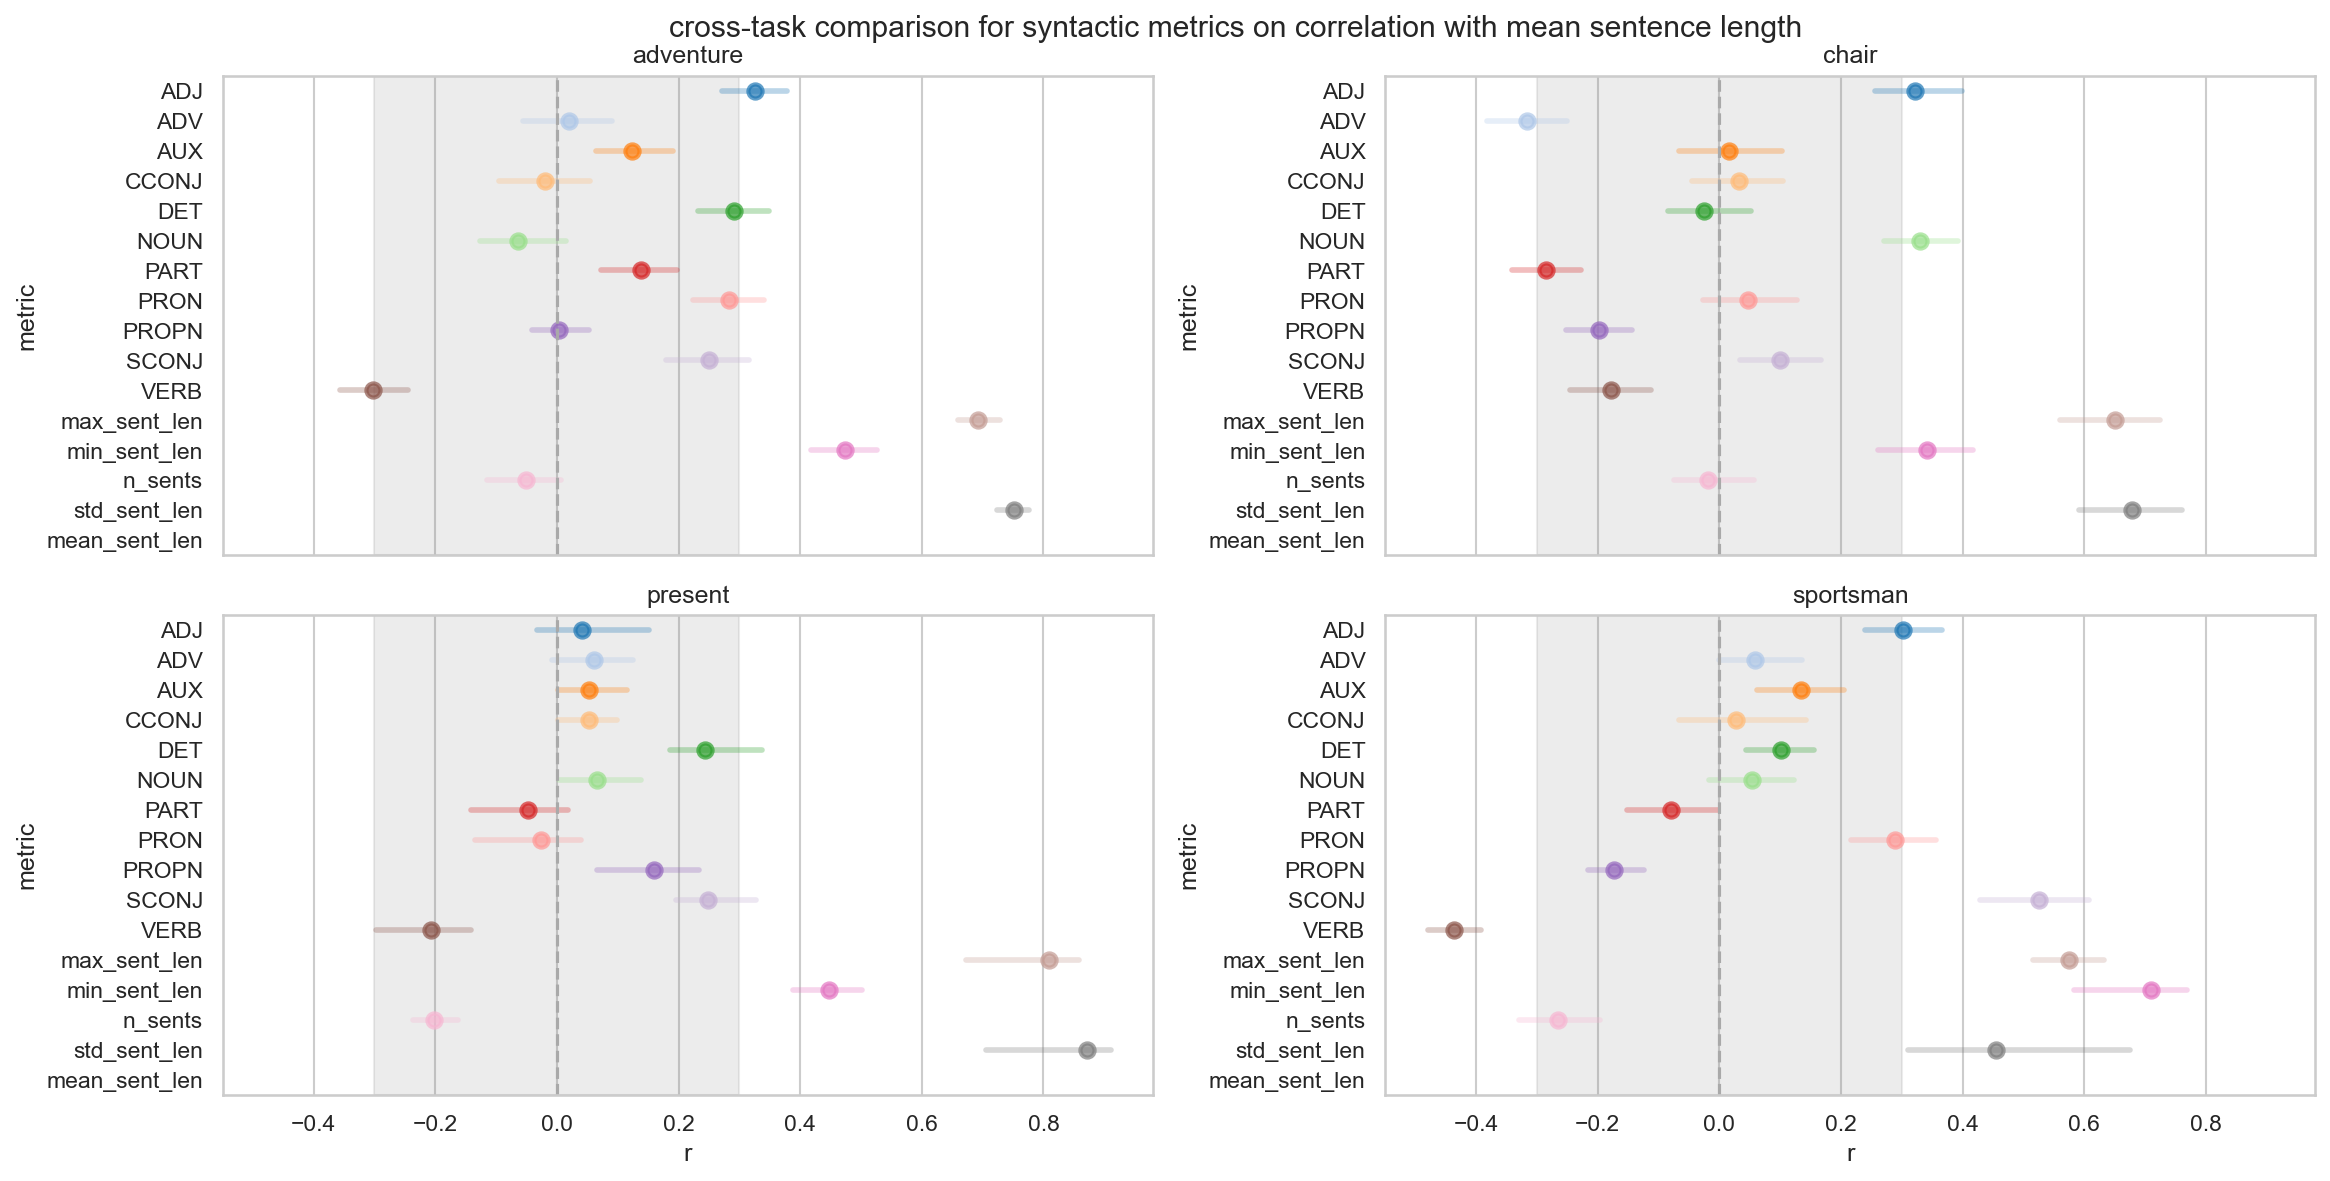
\includegraphics[width=1.1\textwidth, center]{Figures/chapter_4/syntactic/ru_corr_len.png} 
\captionsetup{width=\textwidth}
\caption[Syntactic Metrics: Russian, Length Correlation]{\label{fig:results:syntactic:ru:corr_len} Pearson's r correlation coefficient with mean sentence length for the syntactic metrics on the Russian dataset across tasks. Grey indicates the values below 0.3.}
\end{figure}

Overall, on the Russian sample, the number of sentences was the strongest metric, being the only one, that correlated with symptom scales on all tasks. The rate of PART was positively correlated with symptom severity on three of the four tasks. As could be expected, mean sentence length served as a good baseline on only two of the tasks (chair and	present), and maximal sentence length performed on the same tasks, though it correlated with fewer subscales that mean sentence length. As for, CCONJ, DET, and NOUN rates, each only performed on one of the tasks, and the same is true of standard deviation in mean sentence length.

\subsection{Cross-Linguistic Comparison}
In both languages, PART rate correlated positively with PANSS scales, and similarly in both languages mean, maximal, and standard deviation sentence length correlated negatively with PANSS scales, with mean sentence length performing better on the German sample, as could be expected. CCONJ rate correlated negatively both on the German and the Russian samples, though for the latter only on one scale for one task. AUX rate correlated negatively only on the German sample, and NOUN and DET did so only on the Russian sample, both on only one task. Similarly, the number of sentences correlated negatively with PANSS scales only on the Russian sample.



%-----------------------------------
%	section 6
%-----------------------------------
\clearpage
\section{Graph-Based Methods}
\label{sec:results:clinical:graph}
This section covers the performance of co-occurrence graph-based metrics, number of nodes (N), number of edges (E), largest connected component (LCC), largest strongly connected component (LSC), number of parallel edges (PE), number of loops of length one (repeated lemmas), two, and three (L1, L2, L3), average node degree (degree average), and standard deviation in the node degree (degree std).  


\subsection{German}
Among the graph metrics, shown in figure \ref{fig:results:graph:de}, four correlated negatively with negative symptom scales, as well as PANSS general and total scores, namely, the largest connected and strongly connected component size as well as the number of nodes and edges. 

\begin{figure}[h!]
    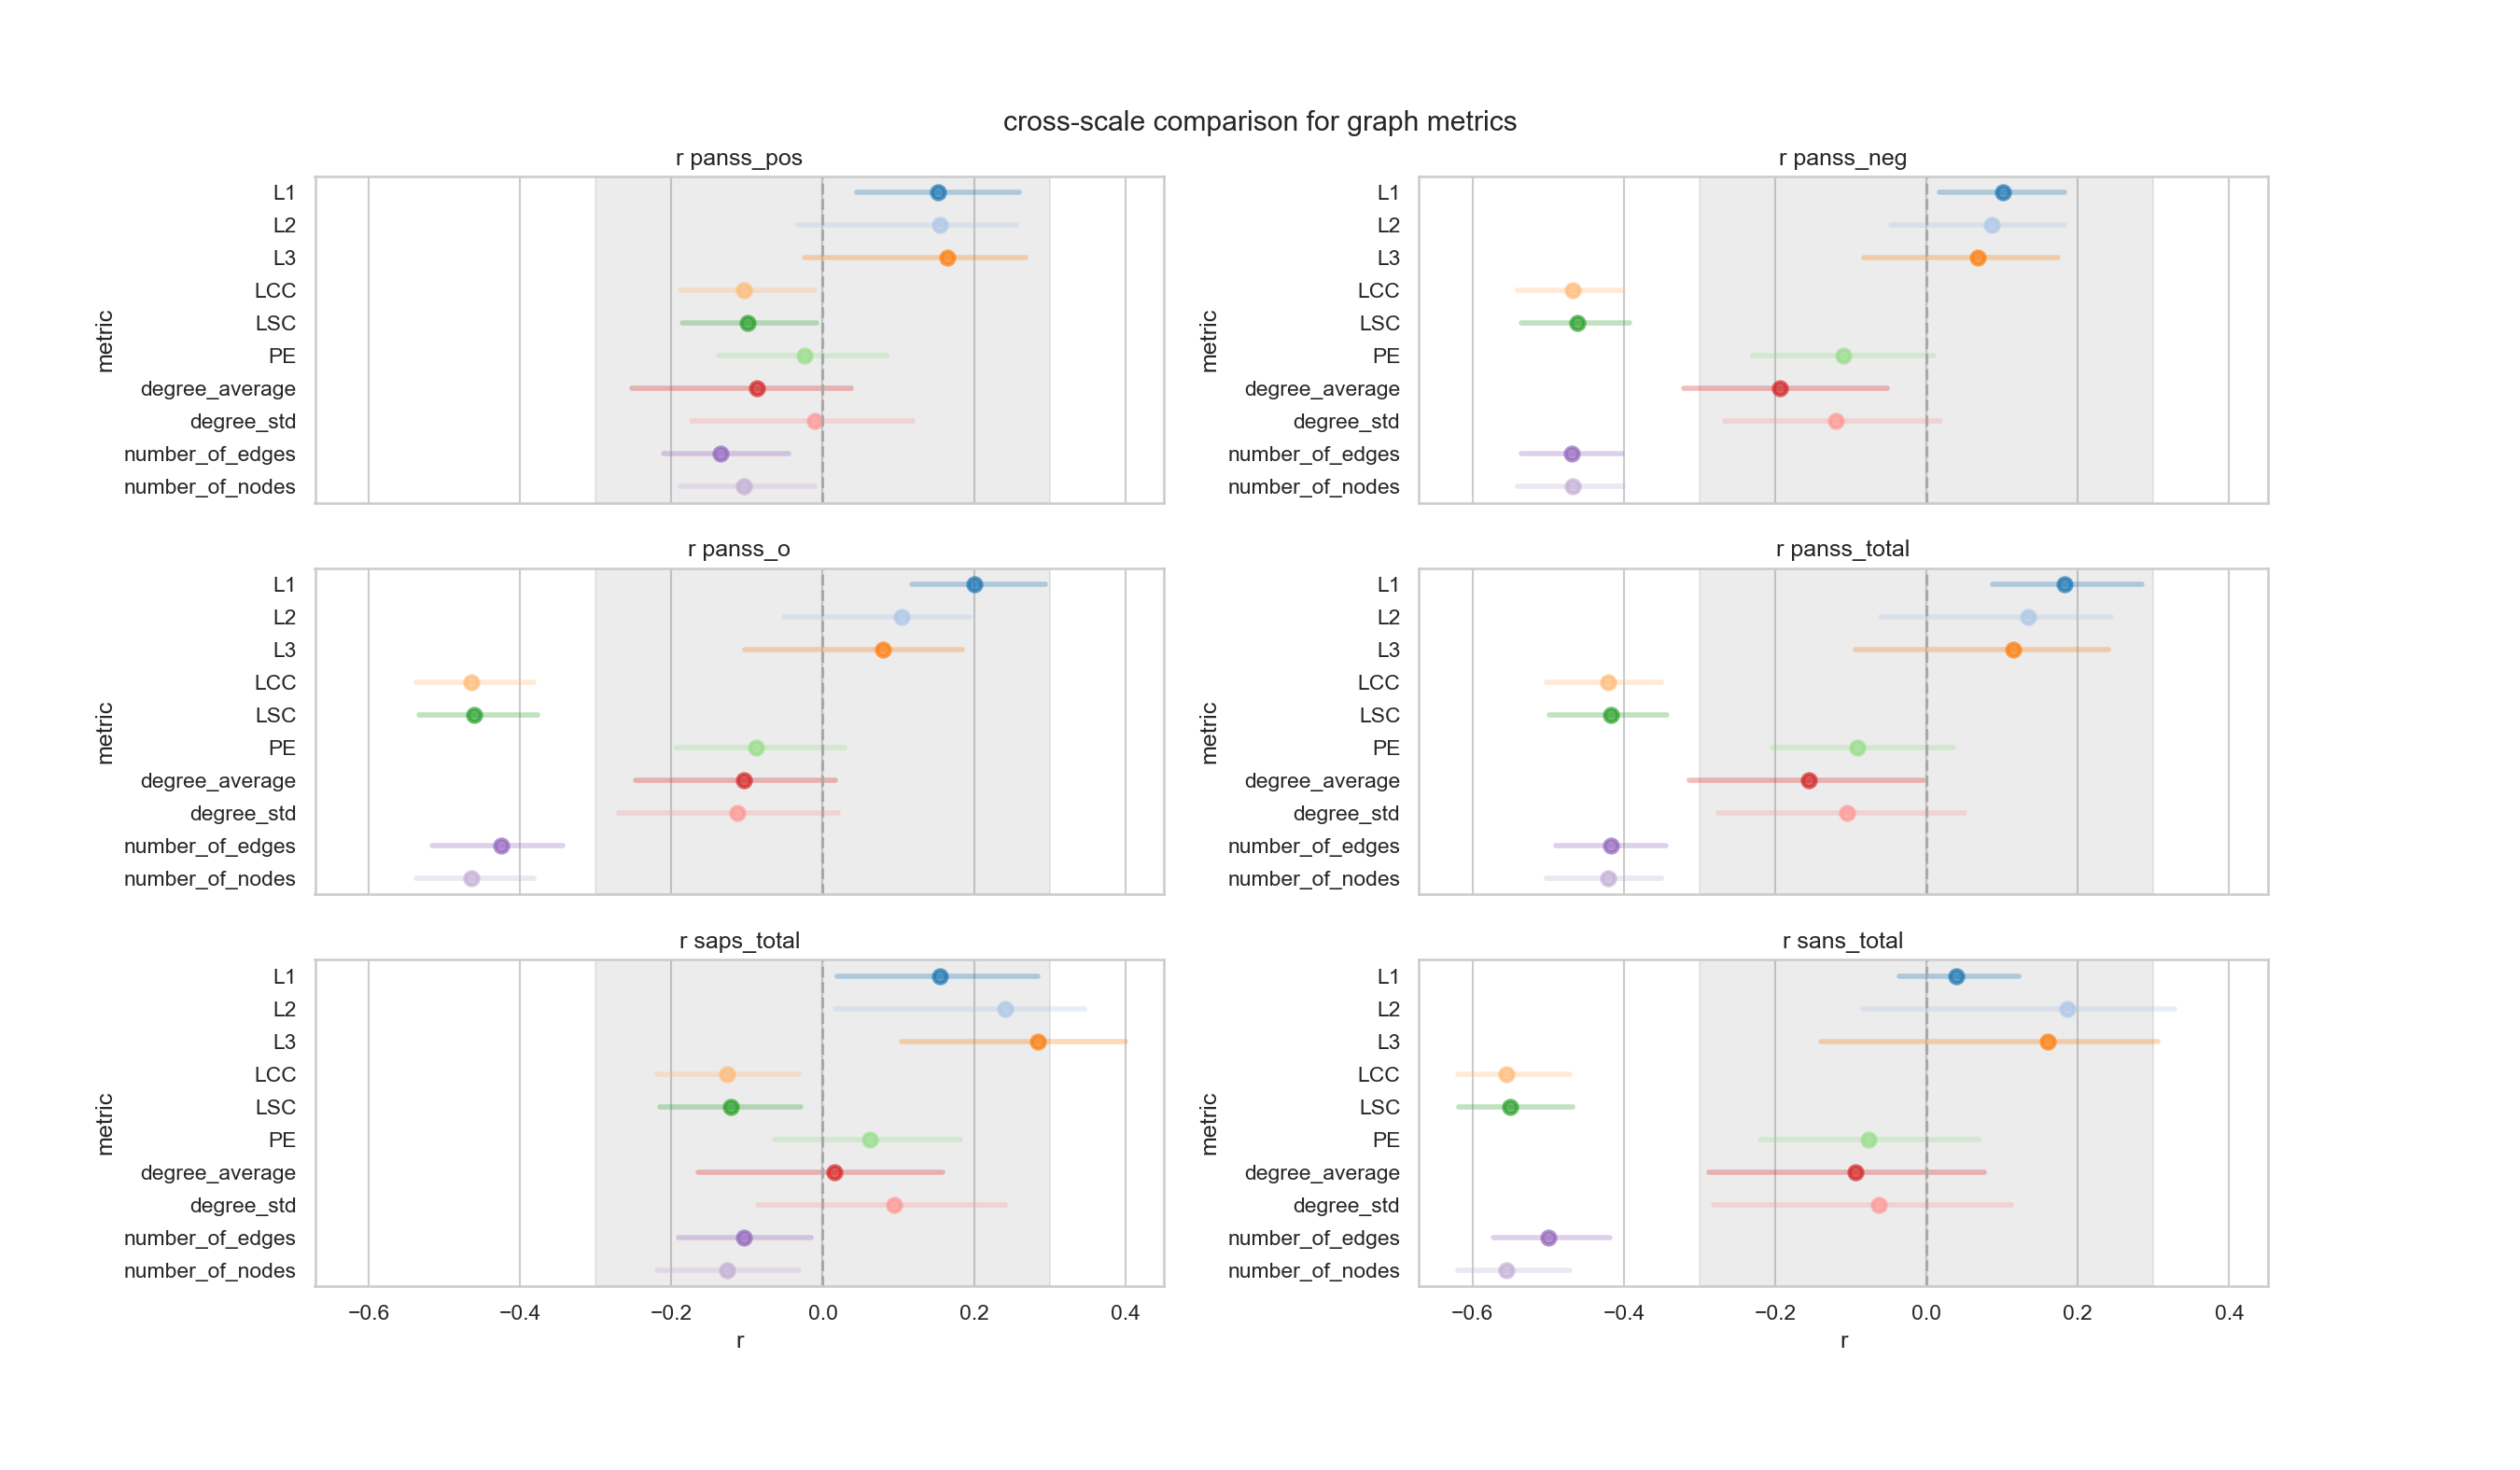
\includegraphics[width=1.2\textwidth, center]{Figures/chapter_4/graph/de_scale_r.png} 
\captionsetup{width=\textwidth}
\caption[Graph Metrics: German]{\label{fig:results:graph:de} Pearson's r correlation coefficient with each scale for the graph-based metrics on the German dataset. Grey indicates the values below the 0.3 threshold in absolute value.}
\end{figure}

Figure \ref{fig:results:graph:de:ttest} shows the strength of correlation with mean sentence length and the power of bidirectional t-test, with the patterns corresponding very closely between the two graphs. The metric values were calculated for moving window of size 100, to avoid direct correlation with verbosity, yet there was still a significant correlation with mean sentence length for all the metrics that performed well on t-test and the psychiatric scales, i.e. LCC, LSC, N, and E. 

\begin{figure}[ht!]
    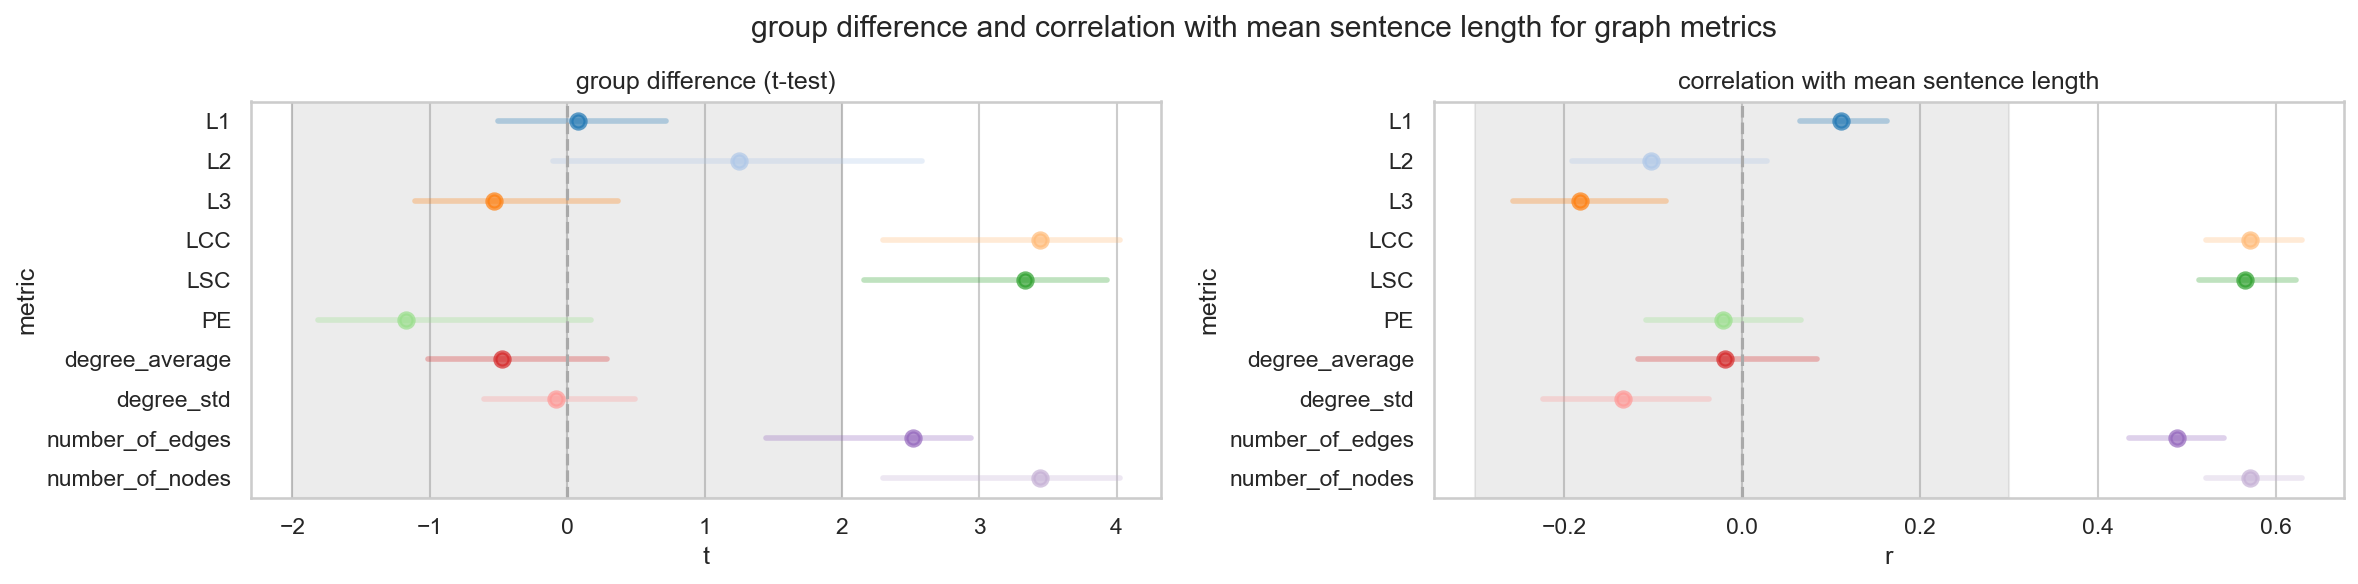
\includegraphics[width=\textwidth, center]{Figures/chapter_4/graph/de_t_test_corr_len.png} 
\captionsetup{width=\textwidth}
\caption[Graph Metrics: German (T-Test)]{\label{fig:results:graph:de:ttest} T-test and Pearson's r correlation coefficient with mean sentence length for the graph-based metrics on the German dataset. Grey indicates the values below 2 for t score and below the 0.3 threshold in absolute value for correlation coefficient.}
\end{figure}

\clearpage
\subsection{Russian}
Figure \ref{fig:results:graph:ru:ad} shows the performance of graph-based metrics on adventure task. The largest connected and strongly connected component size as well as the number of nodes and edges correlated negatively with PANSS general and total scores, and all of these but the number of edges also correlated with PANSS negative.

\begin{figure}[ht!]
    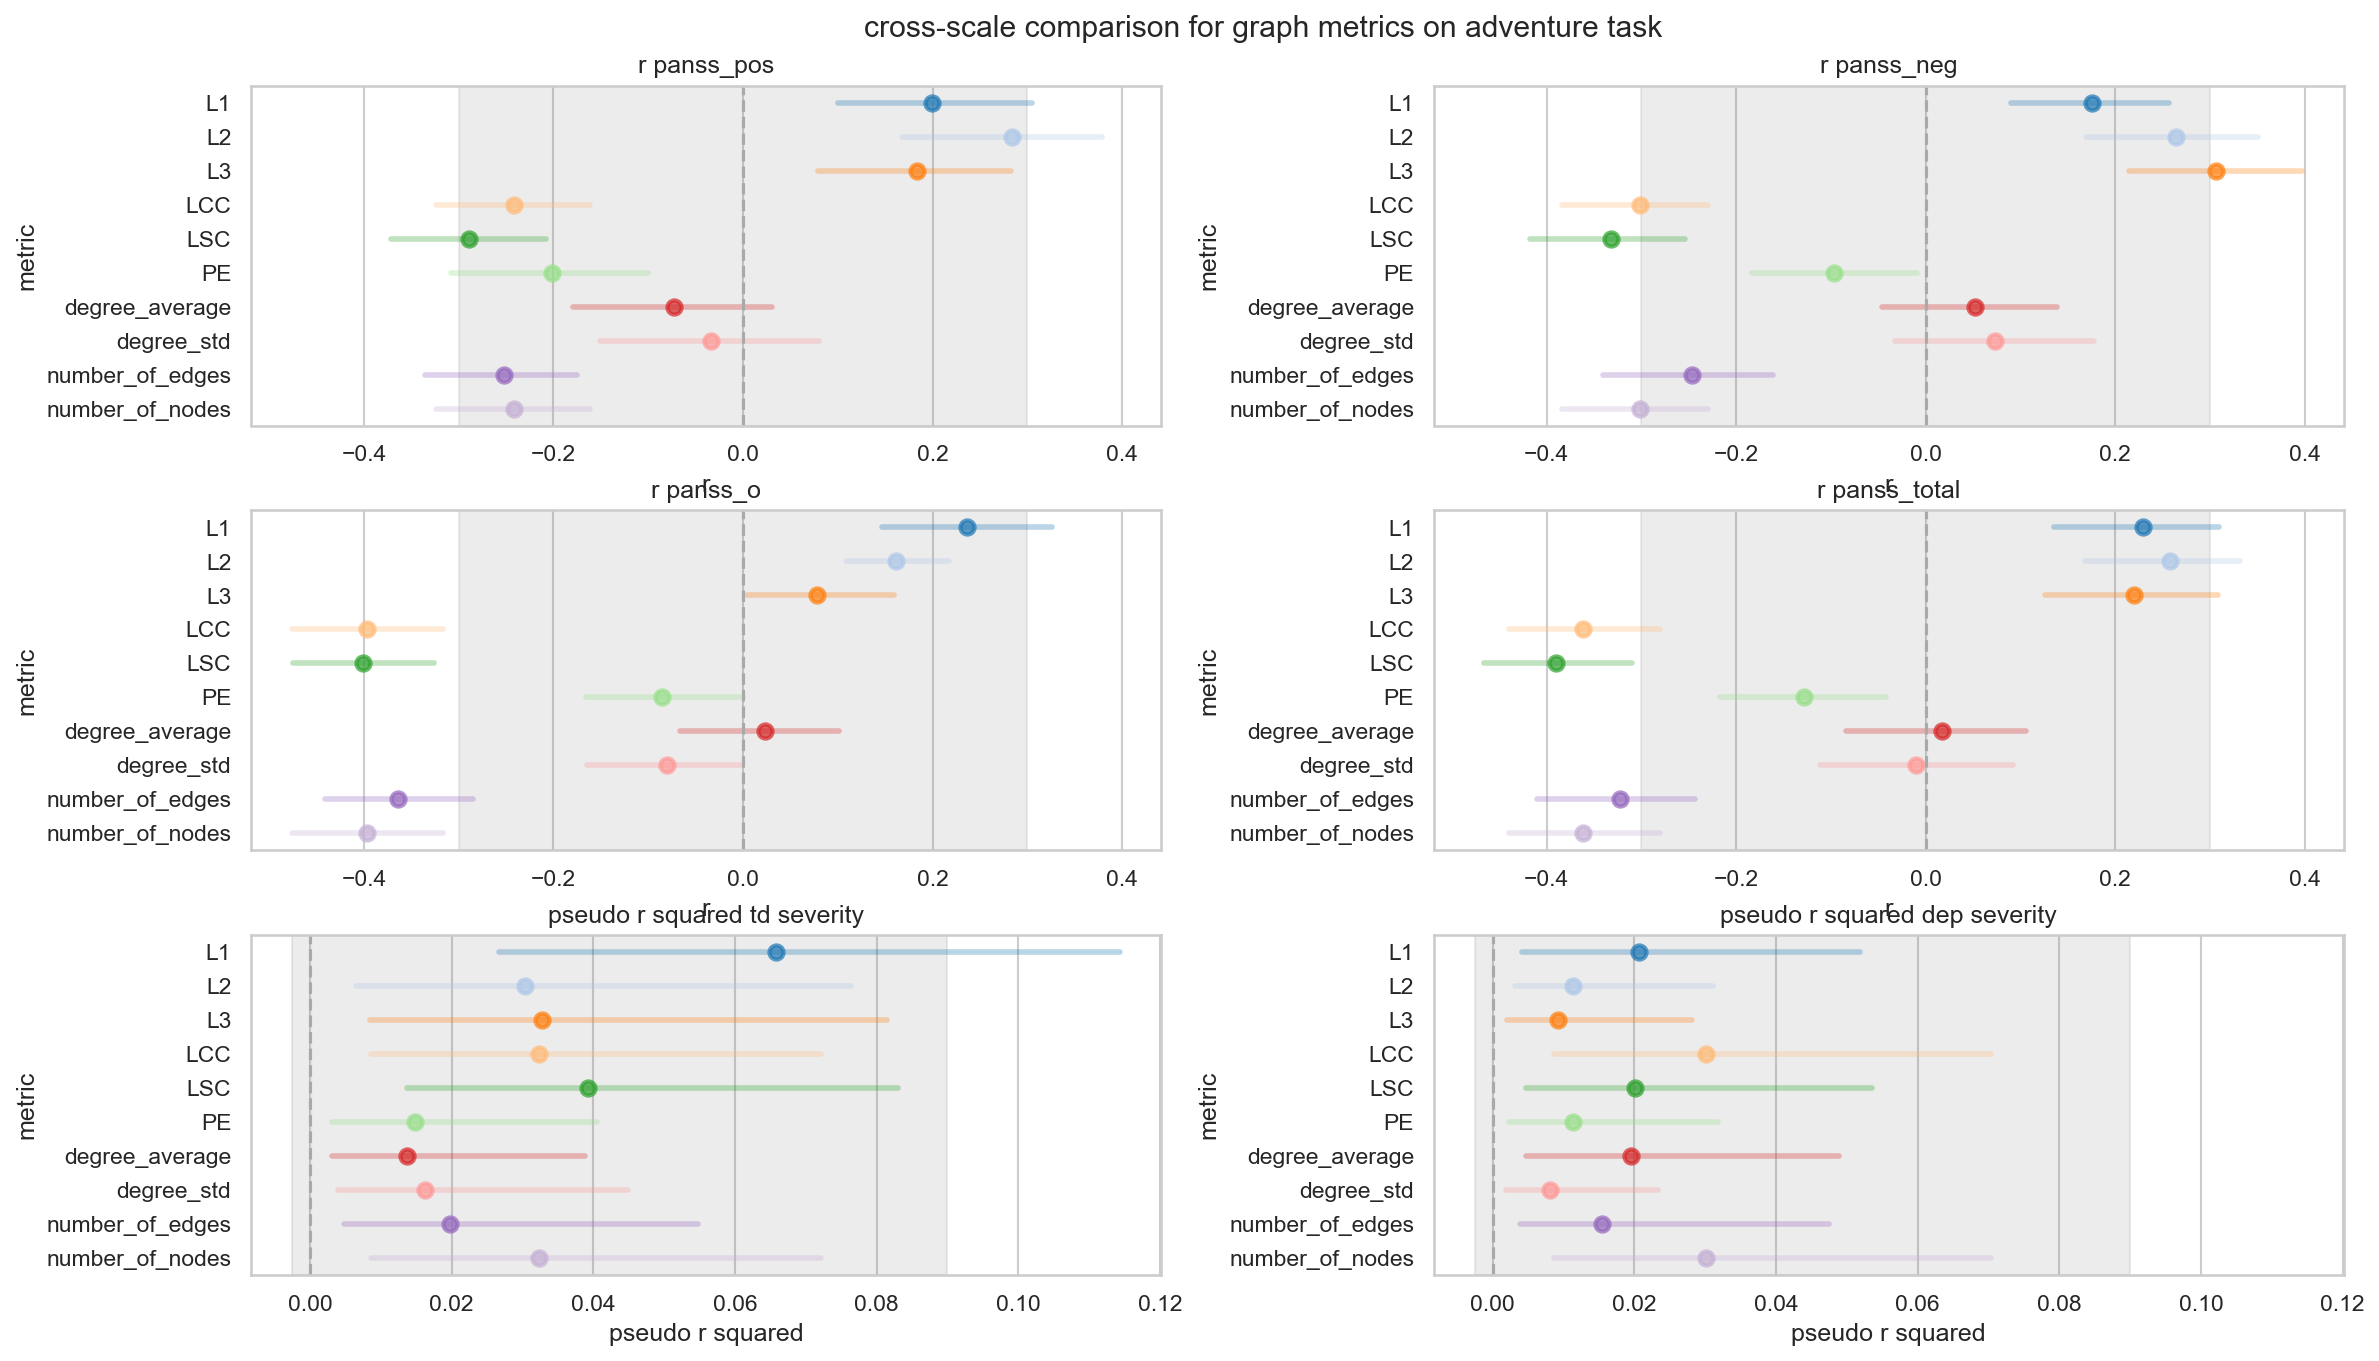
\includegraphics[width=1.1\textwidth, center]{Figures/chapter_4/graph/ru_adventure_scale_r.png} 
\captionsetup{width=\textwidth}
\caption[Graph Metrics: Russian, Adventure Task]{\label{fig:results:graph:ru:ad} Pearson's r correlation coefficient and pseudo r squared for each scale for the graph-based metrics on the Russian dataset, adventure task. Grey indicates the values below the 0.3 threshold in absolute value or pseudo r squared below 0.09.}
\end{figure}

\clearpage
Figure \ref{fig:results:graph:ru:ch} shows the performance of graph-based metrics on chair task. The largest connected and strongly connected component size as well as the number of nodes and edges correlated negatively with all PANSS scales. L3 correlated positively with all PANSS scales and was predictive of TD severity, while PE negatively correlated with PANSS positive and total scores, and was, alongside the number of edges, predictive of depression severity. 

\begin{figure}[ht!]
    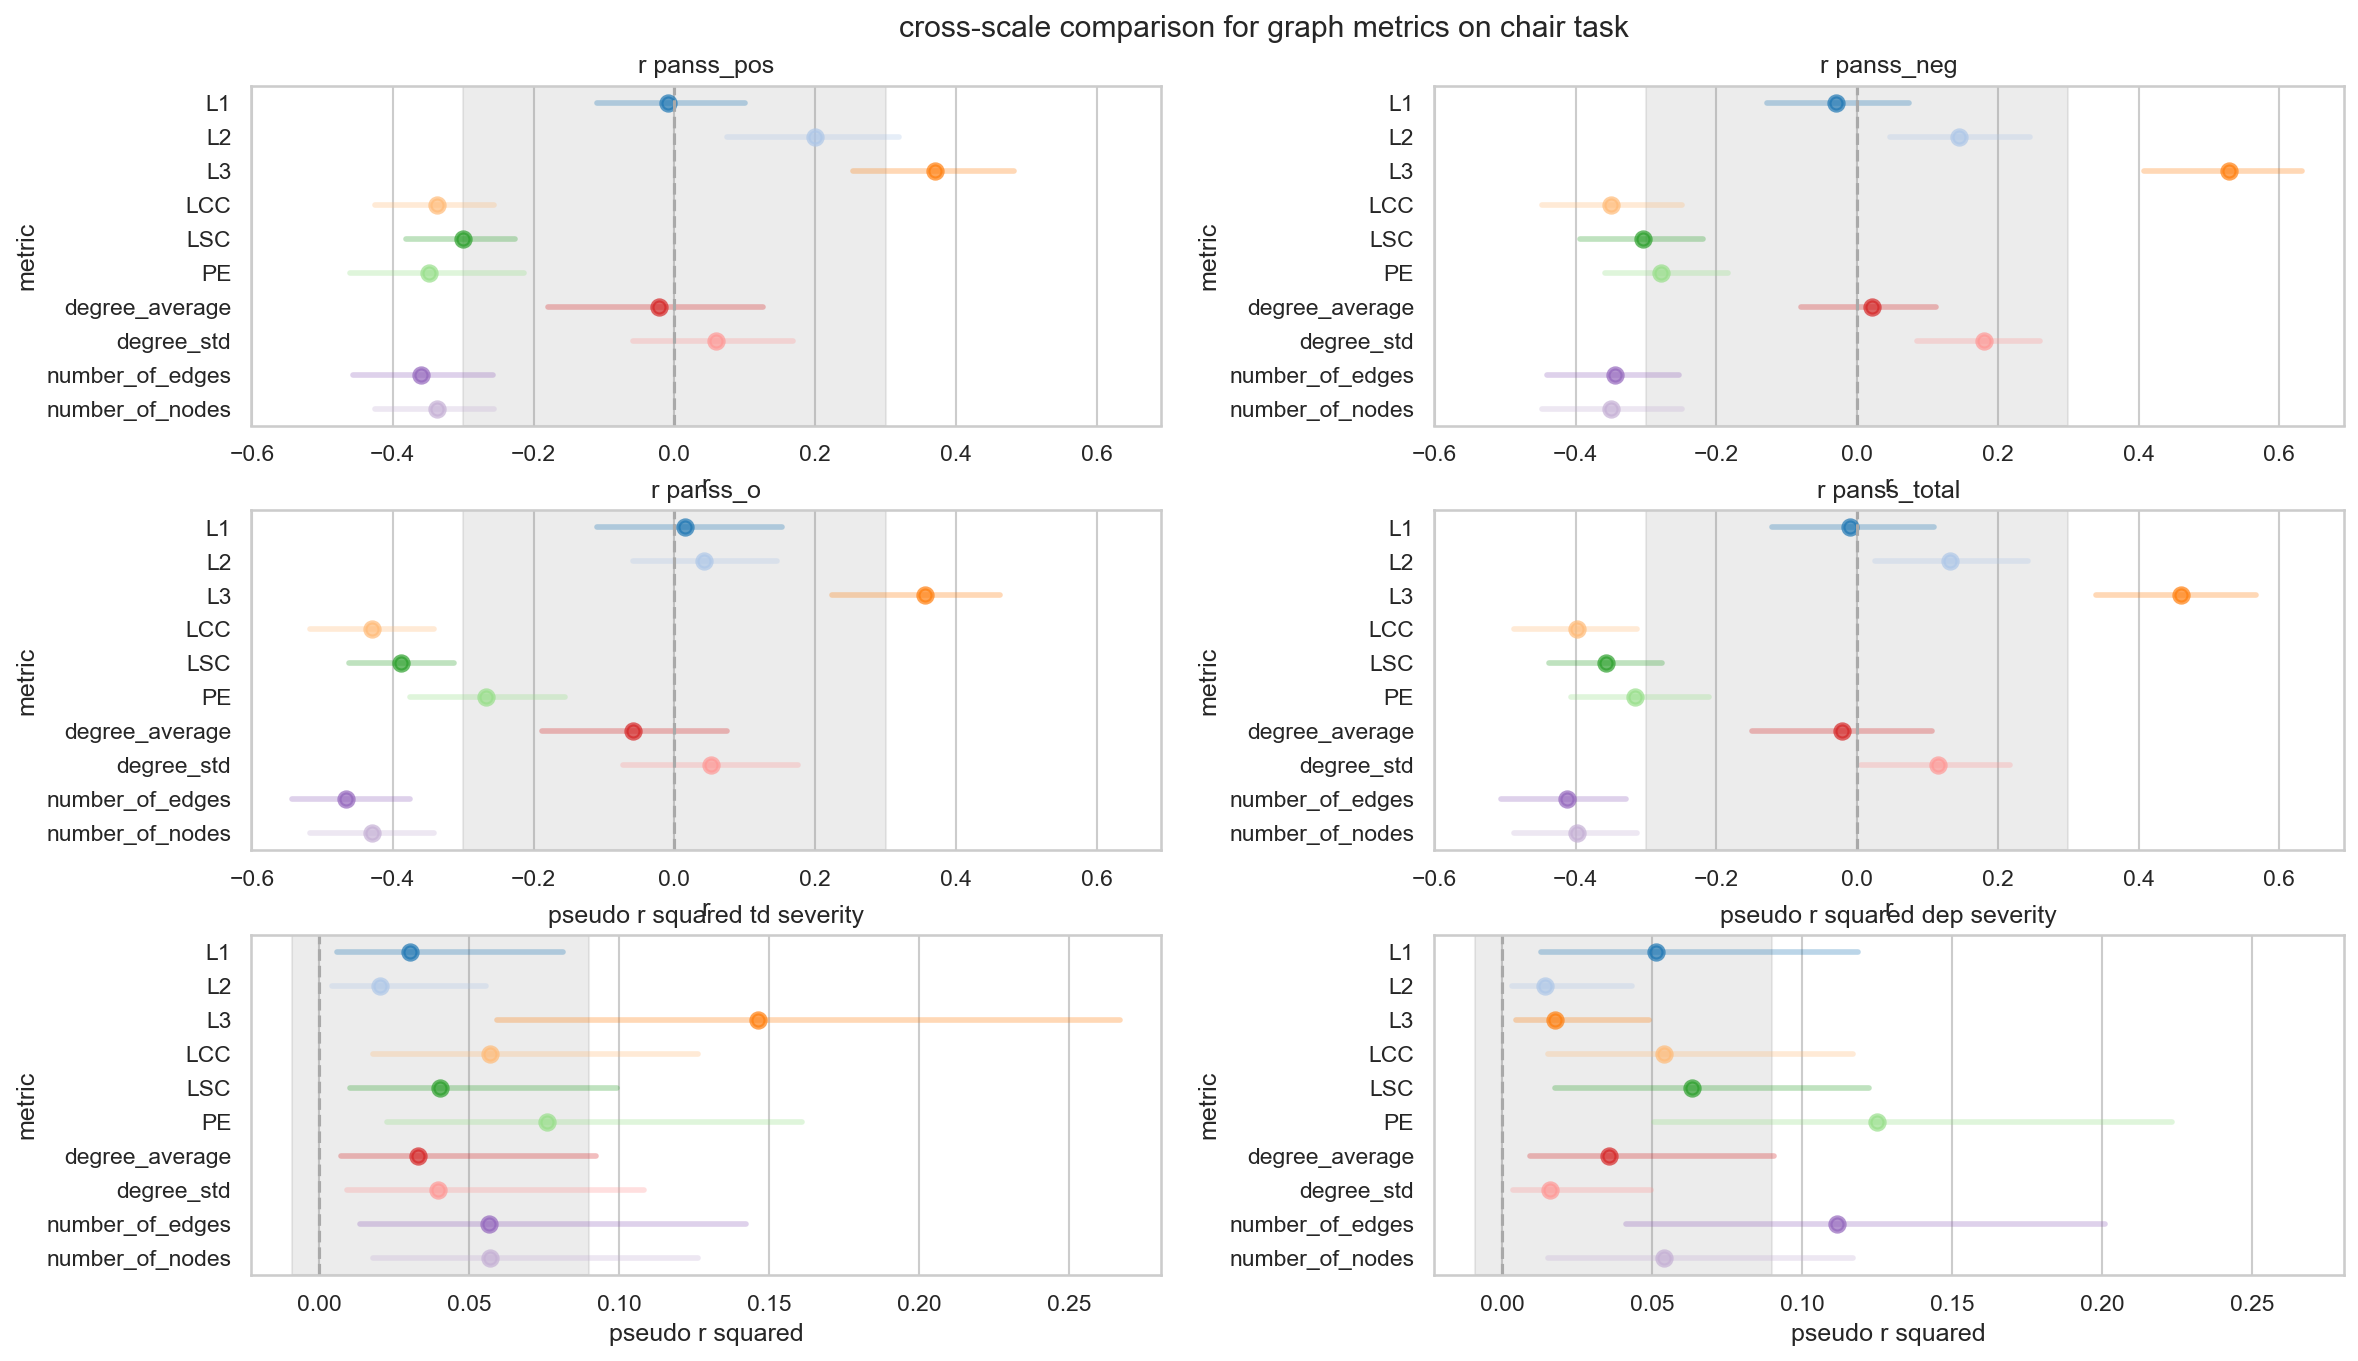
\includegraphics[width=1.1\textwidth, center]{Figures/chapter_4/graph/ru_chair_scale_r.png} 
\captionsetup{width=\textwidth}
\caption[Graph Metrics: Russian, Chair Task]{\label{fig:results:graph:ru:ch} Pearson's r correlation coefficient and pseudo r squared for each scale for the graph-based metrics on the Russian dataset, chair task. Grey indicates the values below the 0.3 threshold in absolute value or pseudo r squared below 0.09.}
\end{figure}

\clearpage
Figure \ref{fig:results:graph:ru:pr} shows the performance of graph-based metrics on present task. The largest connected and strongly connected component size as well as the number of nodes and edges correlated negatively with all PANSS scales and were also predictive of thought disorder severity. Additionally, on present task, average node degree and standard deviation in node degree correlated negatively with PANSS positive and total scores, and average degree was somewhat predictive of TD severity as well.  L1 correlated slightly with PANSS general score.

\begin{figure}[ht!]
    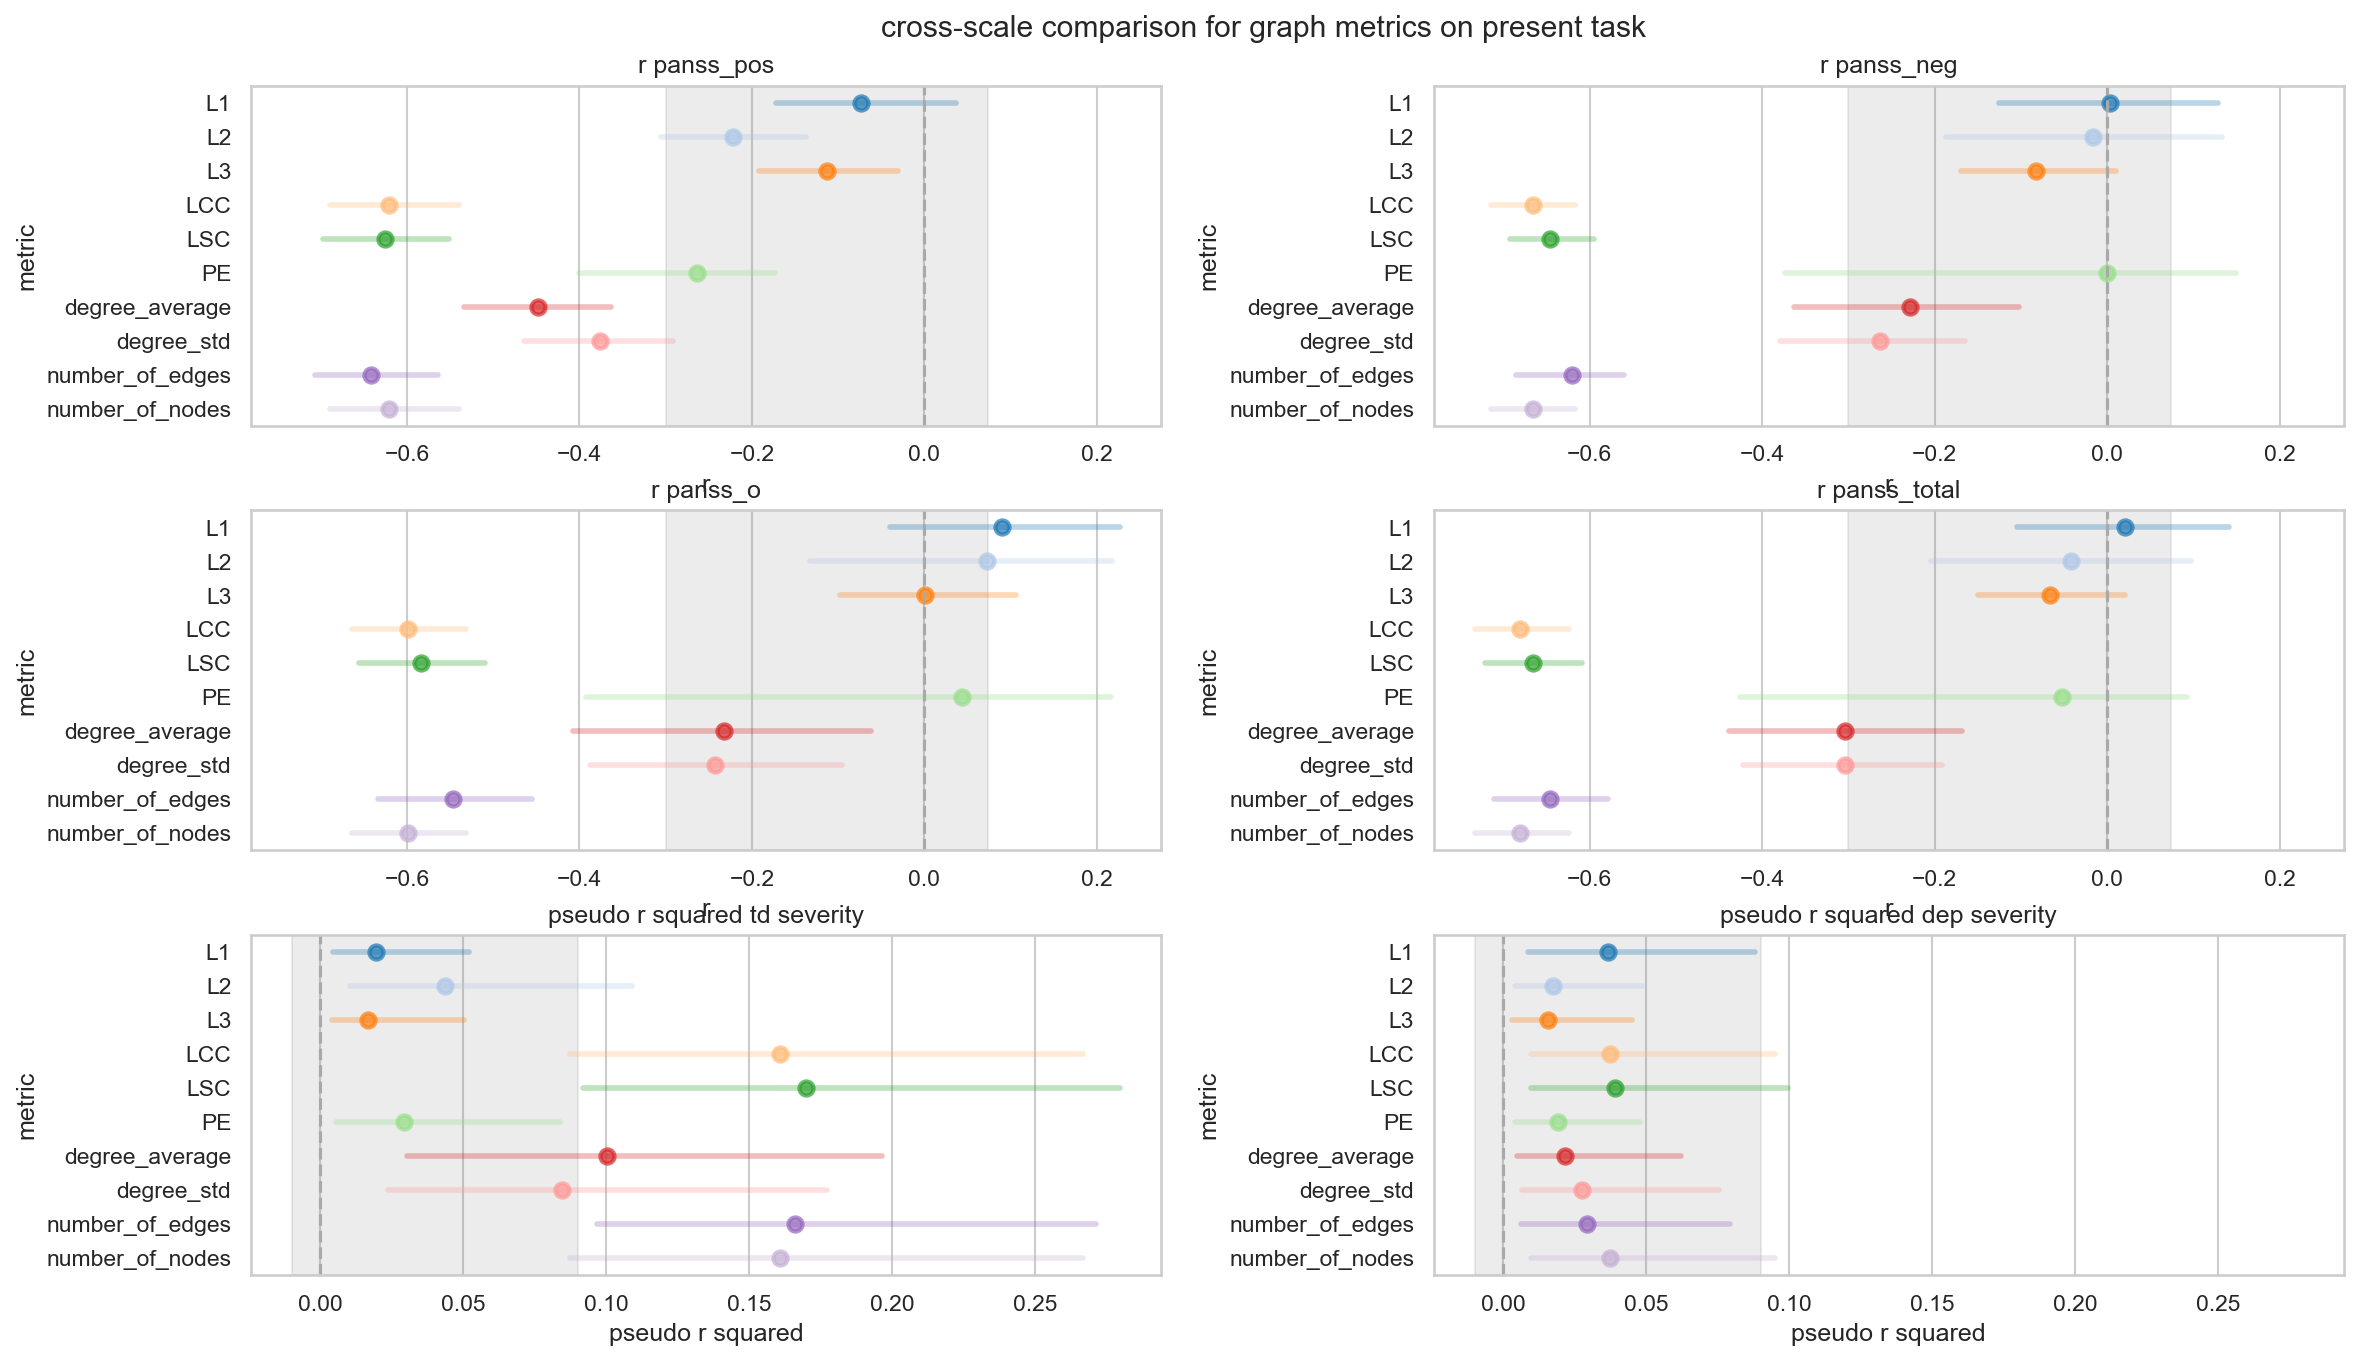
\includegraphics[width=1.1\textwidth, center]{Figures/chapter_4/graph/ru_present_scale_r.png} 
\captionsetup{width=\textwidth}
\caption[Graph Metrics: Russian, Present Task]{\label{fig:results:graph:ru:pr} Pearson's r correlation coefficient and pseudo r squared for each scale for the graph-based metrics on the Russian dataset, present task. Grey indicates the values below the 0.3 threshold in absolute value or pseudo r squared below 0.09.}
\end{figure}

Finally, figure \ref{fig:results:graph:ru:sp} shows the performance of graph-based metrics on sportsman task. As on other tasks, the largest connected and strongly connected component size as well as the number of nodes and edges correlated negatively with all PANSS scales. The number of parallel edges correlated negatively with all PANSS subscales but general and was also predictive of TD severity.

\begin{figure}[ht!]
    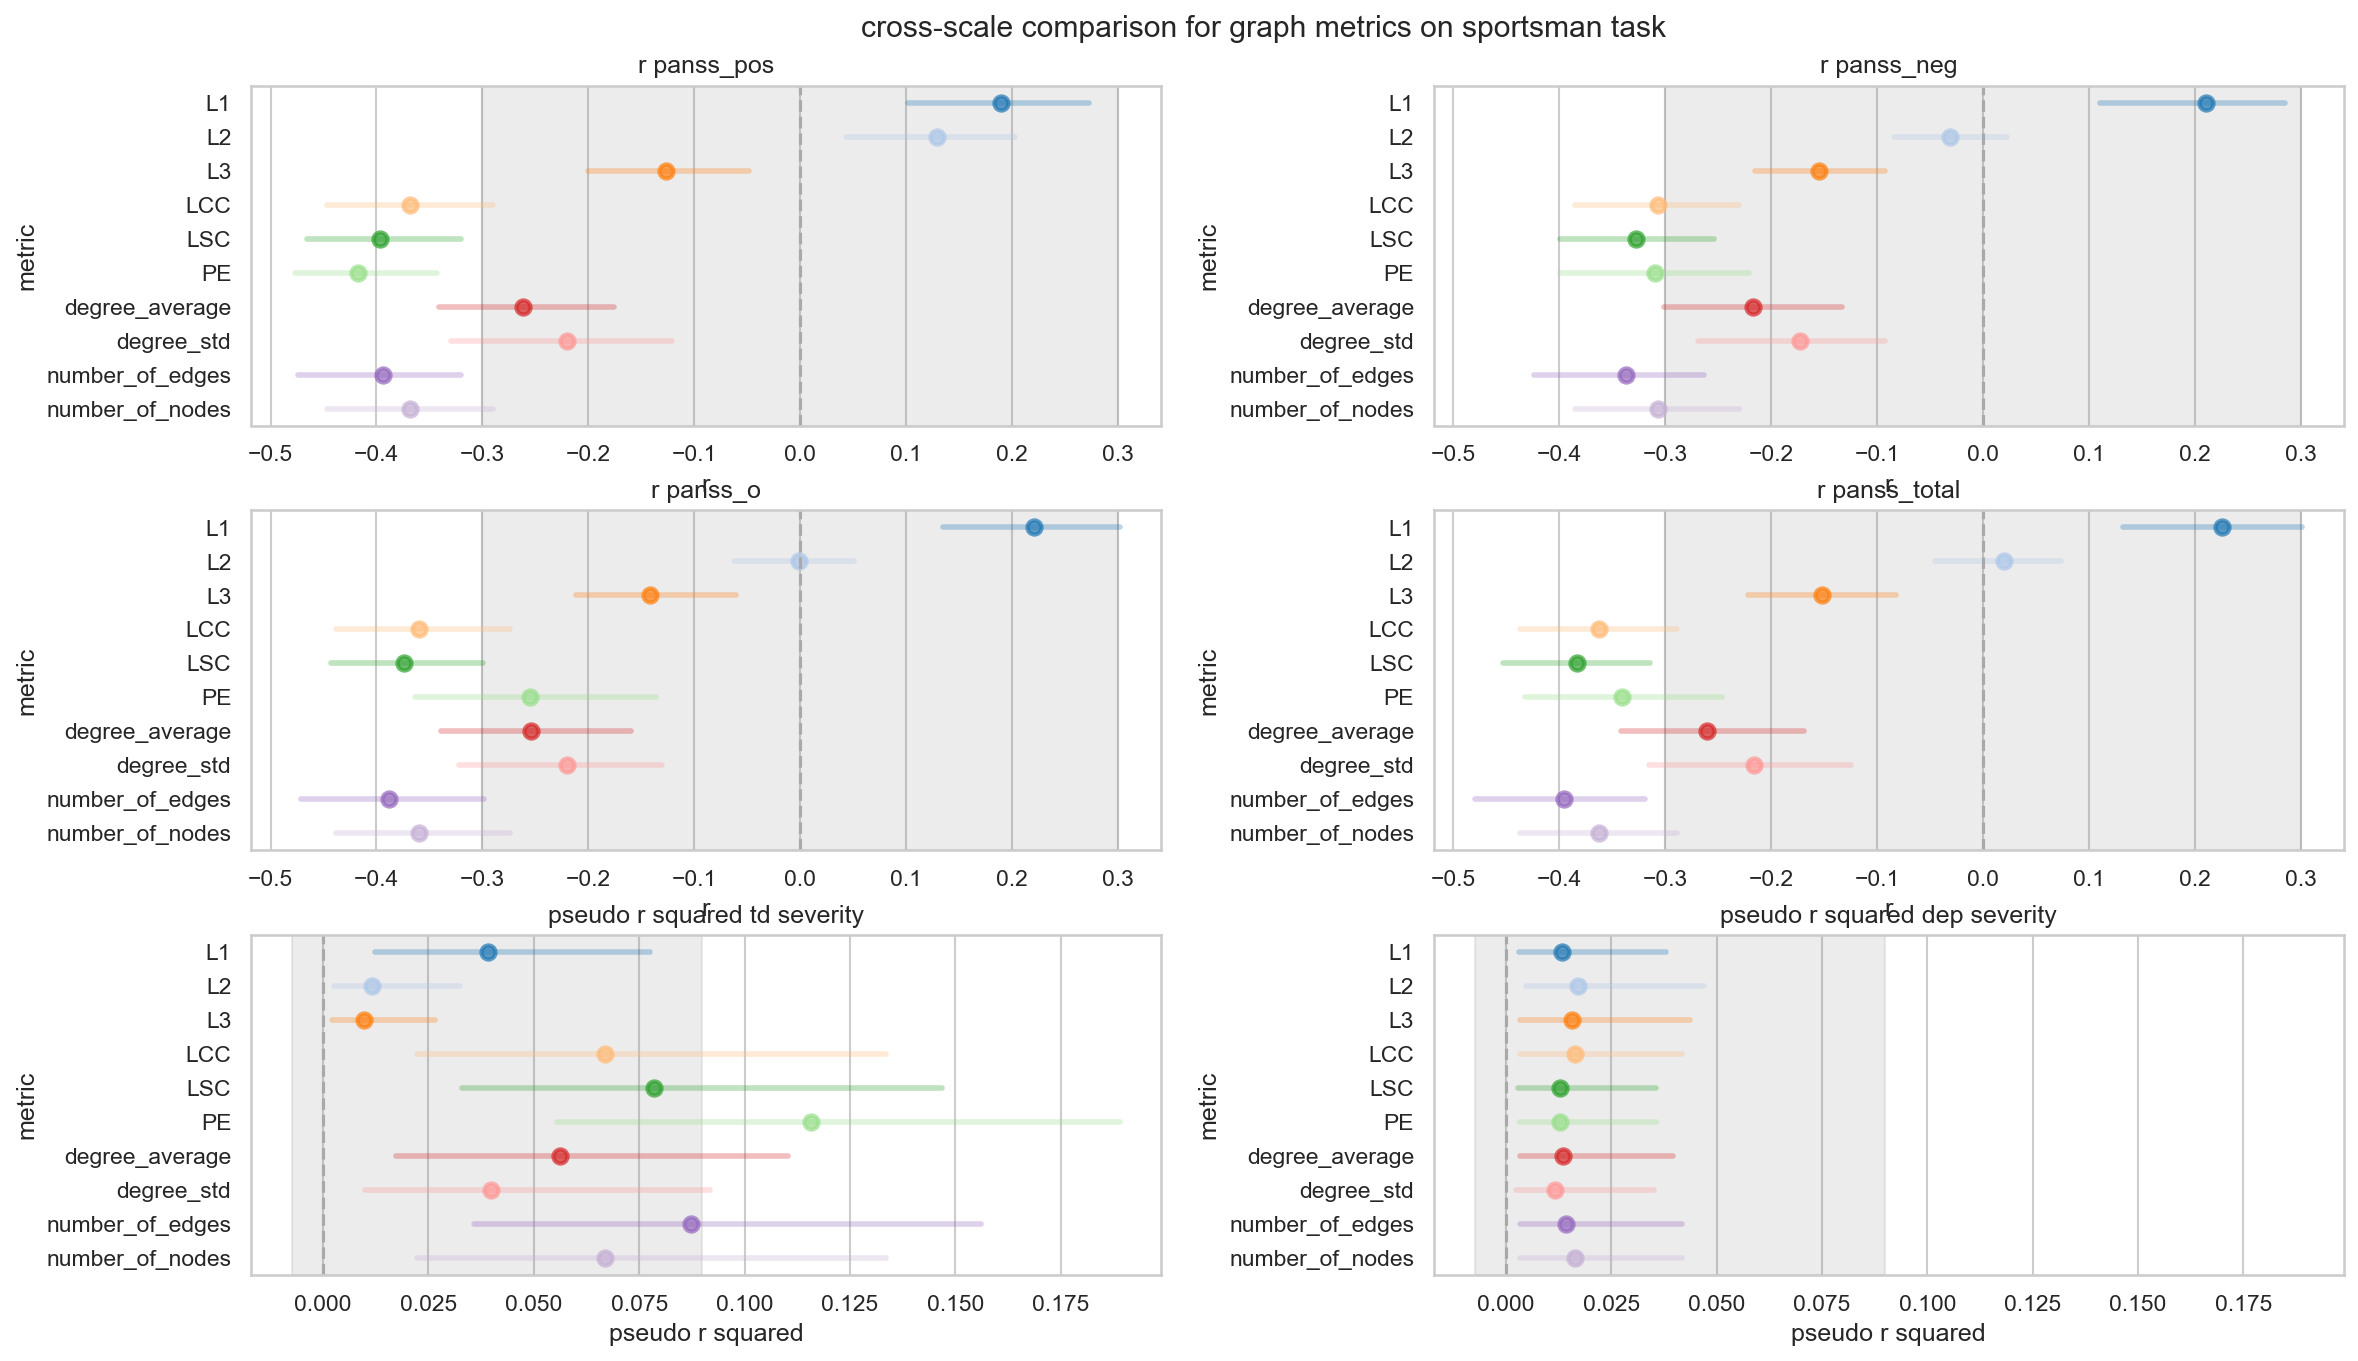
\includegraphics[width=1.1\textwidth, center]{Figures/chapter_4/graph/ru_sportsman_scale_r.png} 
\captionsetup{width=\textwidth}
\caption[Graph Metrics: Russian, Sportsman Task]{\label{fig:results:graph:ru:sp} Pearson's r correlation coefficient and pseudo r squared for each scale for the graph-based metrics on the Russian dataset, sportsman task. Grey indicates the values below the 0.3 threshold in absolute value or pseudo r squared below 0.09.}
\end{figure}


\begin{figure}[ht!]
    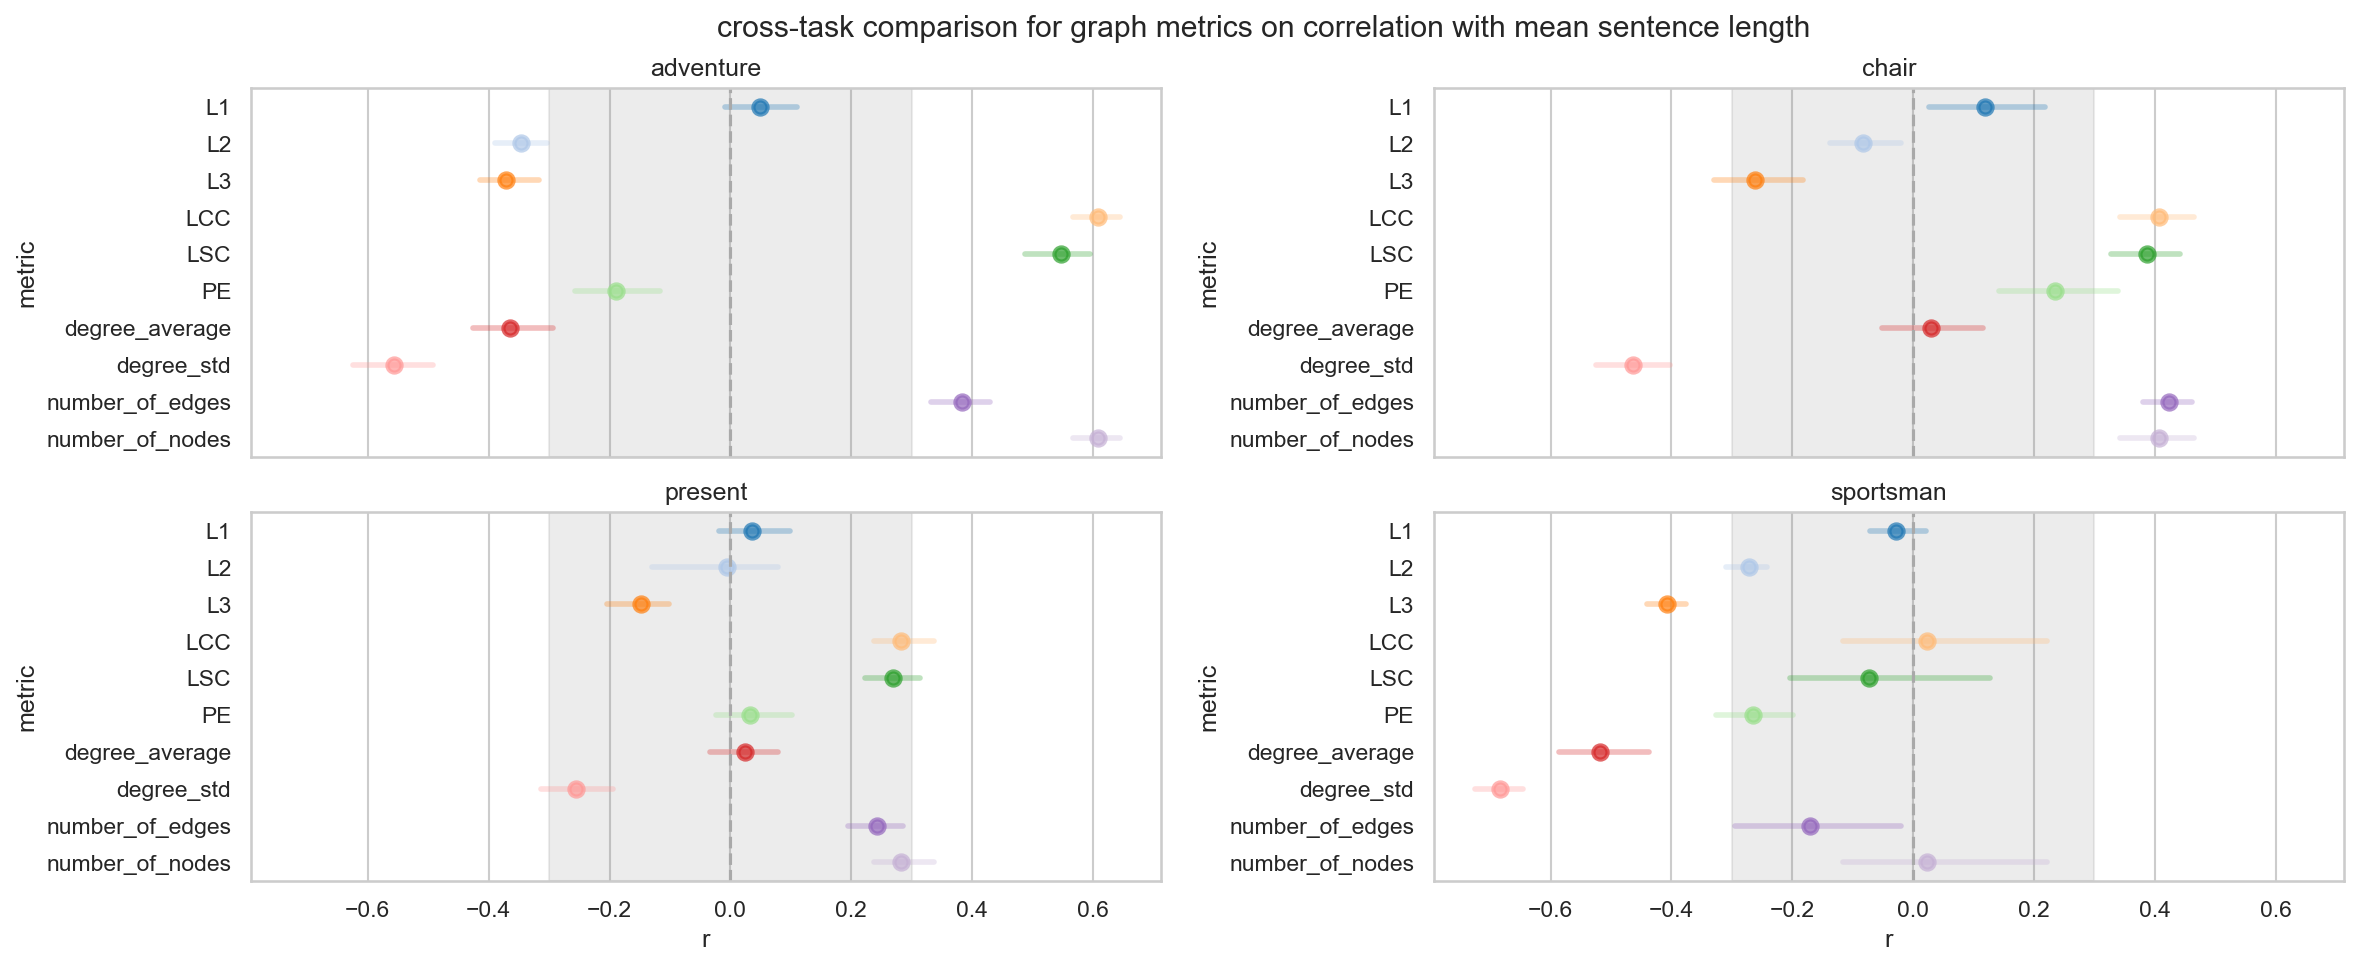
\includegraphics[width=1.1\textwidth, center]{Figures/chapter_4/graph/ru_corr_len.png} 
\captionsetup{width=\textwidth}
\caption[Syntactic Metrics: Russian, Length Correlation]{\label{fig:results:graph:ru:corr_len} Pearson's r correlation coefficient with mean sentence length for the graph-based metrics on the Russian dataset across tasks. Grey indicates the values below 0.3.}
\end{figure}

Figure \ref{fig:results:graph:ru:corr_len} shows the strength of correlation with mean sentence length across tasks. 
LCC, LSC, N, and E correlated positively with mean sentence length on adventure and chair tasks. L2 correlated negatively with mean sentence length on adventure task, and L3, average node degree, and standard deviation of node degree did so on adventure and sportsman tasks. The standard deviation of node degree also correlated negatively with mean sentence length on chair task.

Overall, among the graph-based metrics, LCC, LSC, N, and E showed the best performance on the Russian sample, as they correlated with some psychiatric scales across all of the tasks, though they also were correlated with mean sentence length on the two tasks where it could be expected, as they probably depended somewhat on the verbosity. The number of parallel edges performed on two of the four tasks, chair and sportsman, and the average and standard deviation in node degree, as well as loops of size one (lemma repetitions) and three, only performed on one task, namely, present.

\subsection{Cross-Linguistic Comparison}

Both on the German and Russian samples, LCC, LSC, N, and E were negatively correlated with negative and general symptoms scales and were also positively correlated with mean sentence length, though on the Russian sample, this correlation was present only for some tasks. As positive symptoms were more pronounced in the Russian sample, the same metrics were also correlated negatively with PANSS positive scale and on some tasks predictive of TD and depression severity. L1, L3, PE, average node degree, and standard deviation in node degree, were only correlated with symptom scales on the Russian sample.

%-----------------------------------
%	section 7
%-----------------------------------
\clearpage
\section{Language Model-Based Methods}
\label{sec:results:clinical:LM}

This section covers the results of the language model-based metrics for both languages. The metrics included cumulative global coherence (\texttt{cgcoh}), global coherence (\texttt{gcoh}), local coherence (\texttt{lcoh}), second order coherence (\texttt{scoh}), next sentence probability (\texttt{sprob}), and pseudo-perplexity (\texttt{pppl}). The models included BERT and two weighting schemes for word2vec. \texttt{BERT} is denoted as such, \texttt{w2v} stands for word2vec (fasttext), \texttt{glove} stands for GloVe, and \texttt{tf} on figures stands for TF-IDF weighted sentence scheme, while \texttt{avg} for simple sentence averaging. 

\subsection{German}

Figure \ref{fig:results:lm:de} shows the performance of Language Model-based metrics on the German sample.

\begin{figure}[h!]
    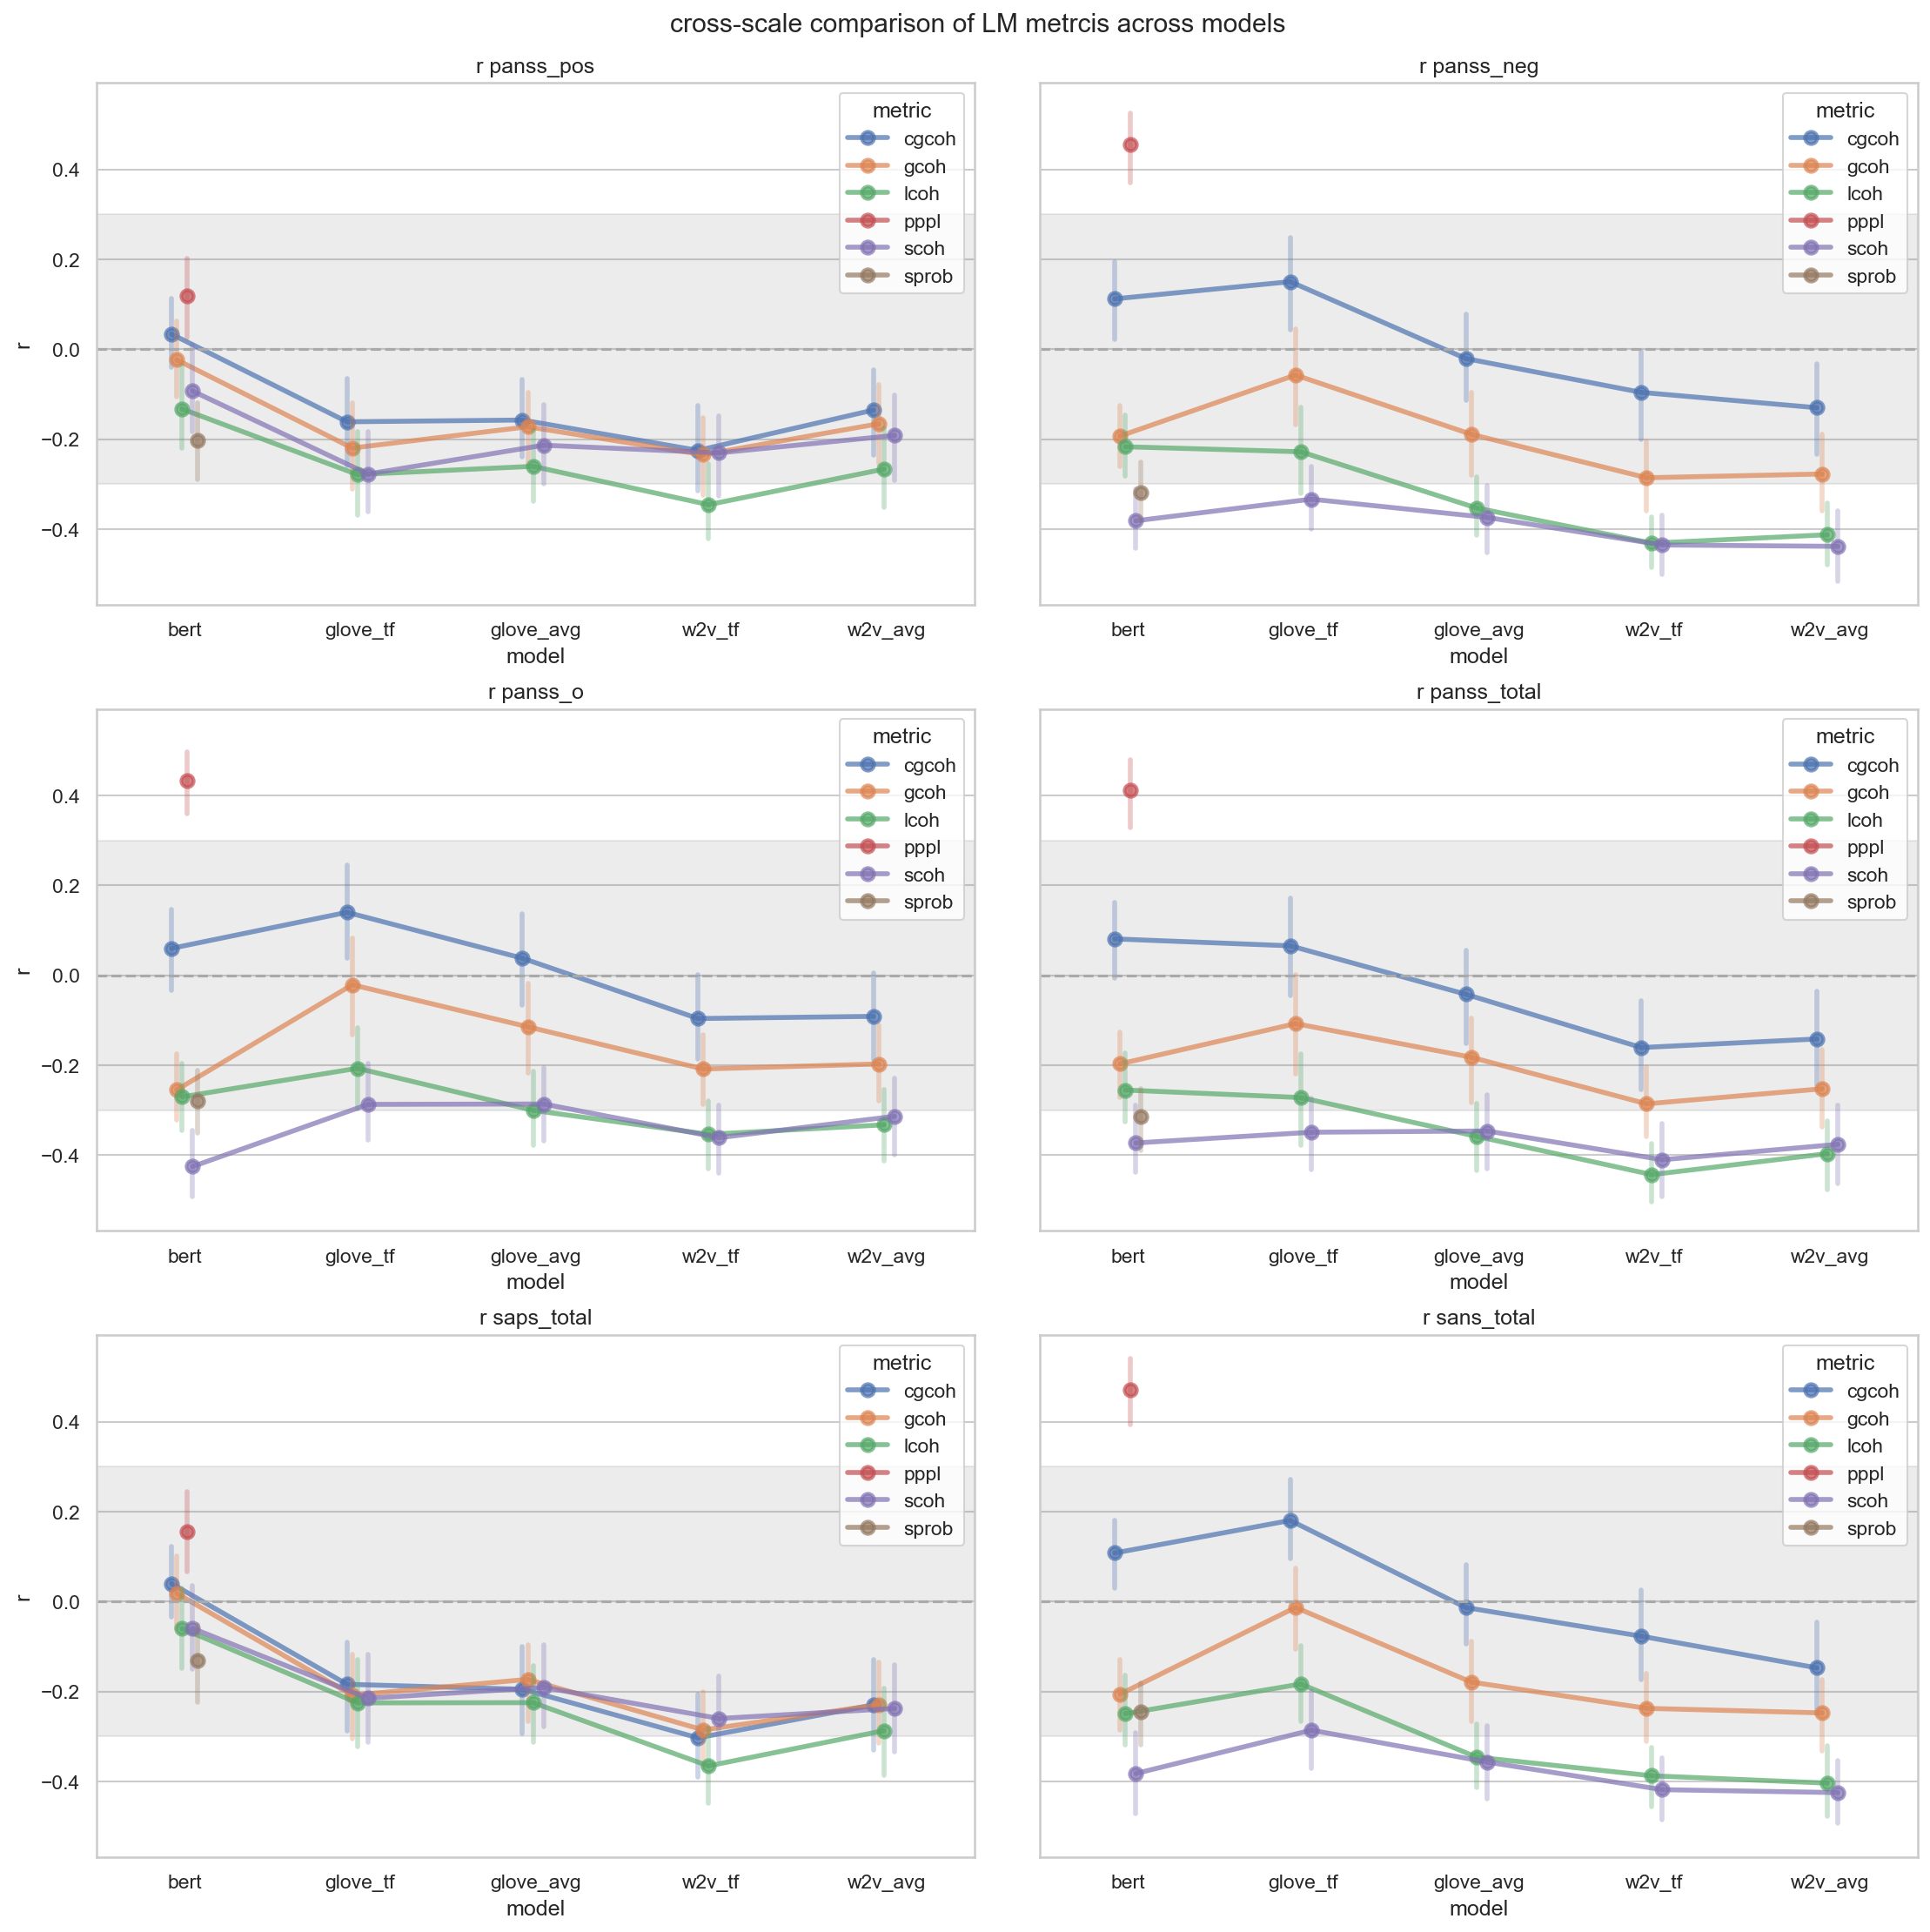
\includegraphics[width=1.1\textwidth, center]{Figures/chapter_4/LM/de_scale_r.png} 
\captionsetup{width=\textwidth}
\caption[LM Metrics: German]{\label{fig:results:lm:de} Pearson's r correlation coefficient with each scale for the LM-based metrics on the German dataset. Grey indicates the values below the 0.3 threshold in absolute value.}
\end{figure}

% hierarchy of metrics
Overall, there was a hierarchy of metrics, with pseudo-perplexity performing the best, positively correlating with negative and general symptom severity. The second-best performing metric was second-order coherence, which correlated negatively across models with negative symptoms and total PANSS, and on all models but averaged GloVe with general PANSS. Local coherence and next sentence probability showed similar levels of performance, with local coherence correlating stronger on word2vec and averaged GloVe, but not BERT, TF-IDF weighted word2vec even correlating negatively with positive symptom severity. Next sentence probability only reached the threshold in negative correlation with PANSS negative and total. Finally, global and cumulative global coherence performed the worst and did not correlate strongly with any of the scales.
% cgcoh    0.120598
% gcoh     0.181313
% sprob    0.248705
% lcoh     0.295024
% scoh     0.311049
% pppl     0.340907

% hierarchy of models
As for the models, on the cosine similarity-based metrics, word2vec showed the best performance with TF-IDF averaging followed by simple averaging, and GloVe, where the pattern was reversed, simple averaging outperforming TF-IDF. For both models, the difference between the averaging schemes was slight. Finally, BERT performed worst for the cosine similarity-based metrics, but the two feature-based metrics performed relatively well.
% bert         0.176137
% glove_tf     0.193866
% glove_avg    0.212054
% w2v_avg      0.263709
% w2v_tf       0.289213

% glove_tf     0.193866
% glove_avg    0.212054
% bert         0.215694
% w2v_avg      0.263709
% w2v_tf       0.289213

Figure \ref{fig:results:lm:de:ttest} shows the results of a bidirectional t-test against the strength of correlation with mean sentence length. Except for pseudo-perplexity, which was somewhat lower in patients than in controls, no metric could differentiate between the groups.

\begin{figure}[ht!]
    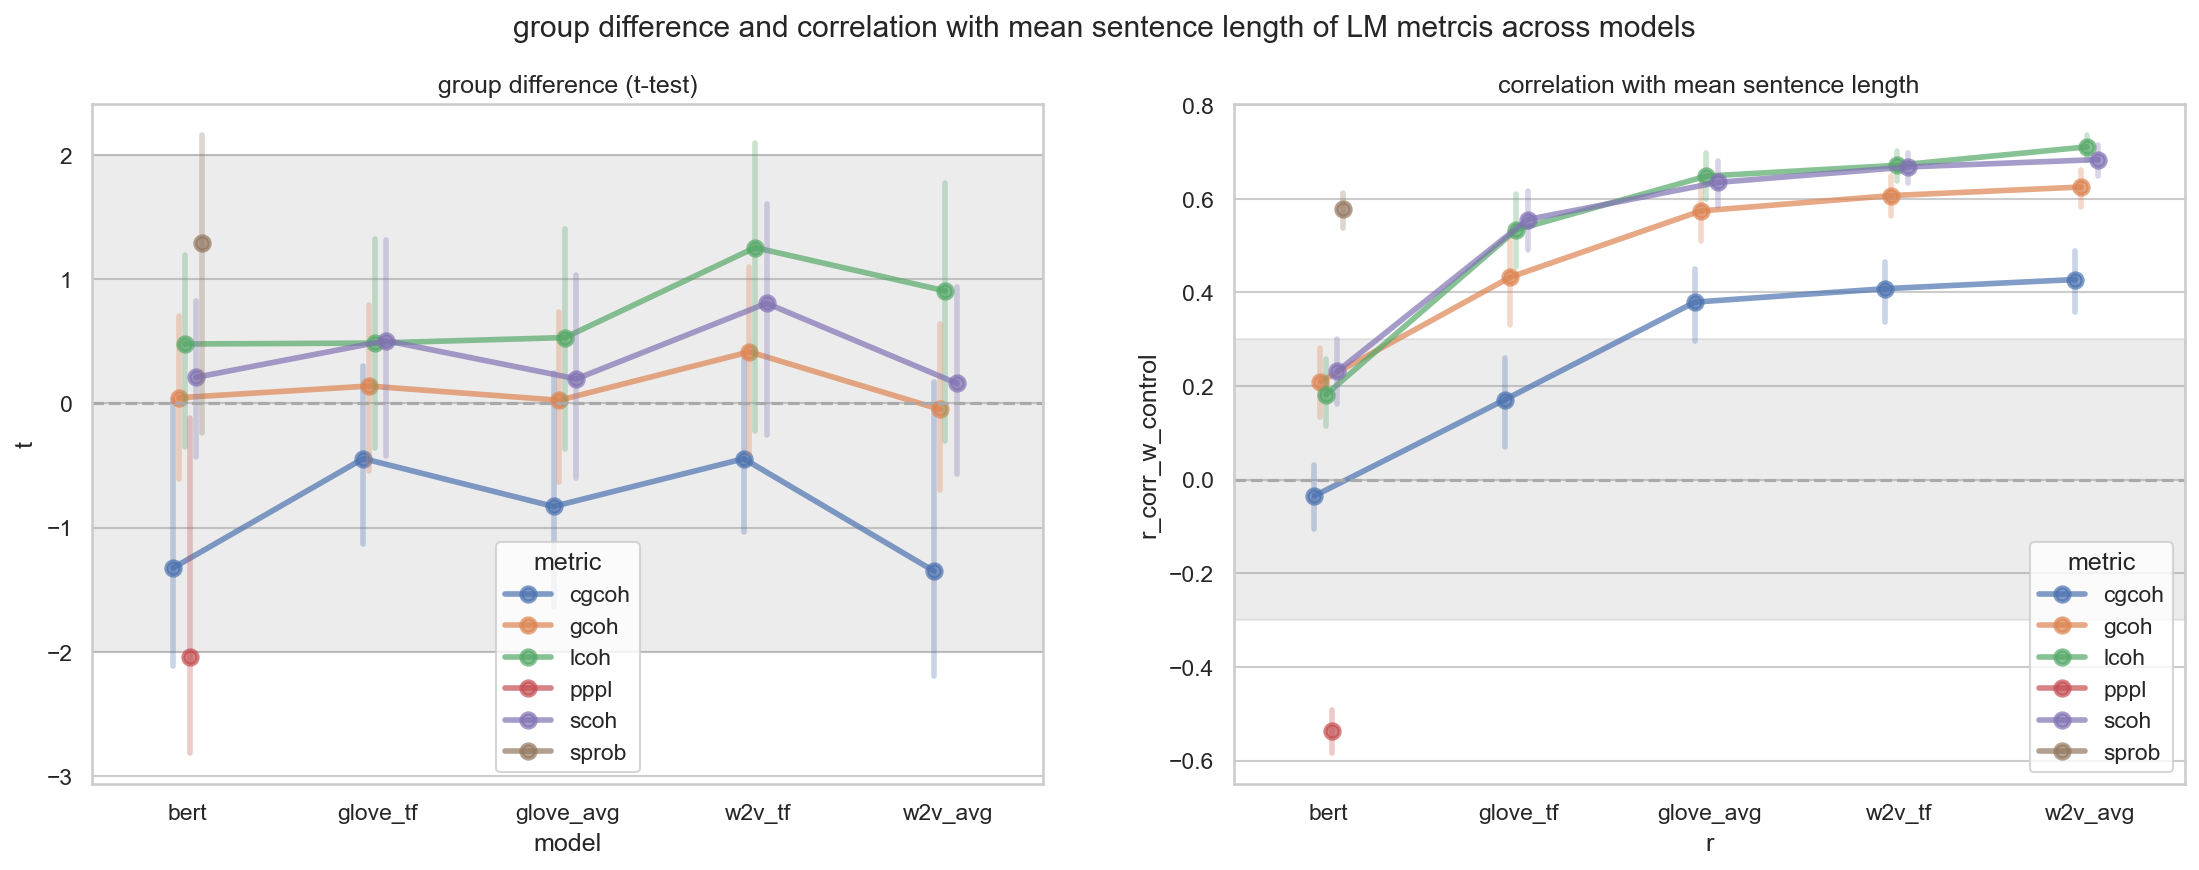
\includegraphics[width=1.1\textwidth, center]{Figures/chapter_4/LM/de_t_test_corr_len.png} 
\captionsetup{width=\textwidth}
\caption[LM Metrics: German (T-Test)]{\label{fig:results:lm:de:ttest} T-test and Pearson's r correlation coefficient with mean sentence length for the LM-based metrics on the German dataset. Grey indicates the values below 2 for t score and below the 0.3 threshold in absolute value for correlation coefficient.}
\end{figure}

% corr len
The cumulative global coherence was least correlated with mean sentence length, followed by global coherence, and then all other metrics. Interestingly, both next sentence probability and pseudo-perplexity were strongly correlated with mean sentence length, though the former was correlated positively and the latter negatively. For the cosine similarity-based metrics, BERT was uncorrelated with mean sentence length. GloVe-based metrics were less correlated than w2v, and the TF-IDF weighted metrics were somewhat less correlated than simple averaged ones. There was an inverse relation trend between overall metric performance and its correlation with mean sentence length, being more pronounced for the correlation with symptom scales, than for the T-test results.

There was an interesting pattern, that cumulative global coherence tended to correlate less negatively (and, in some cases, more positively) than other metrics, and it was followed by global coherence, while local and second-order coherence tended to correlate more negatively with symptom severity.

\subsection{Russian}
Out of the four tasks, on one no LM metric correlated with any of the psychiatric scales, while on the other three, there was some predictive power.

\clearpage
Figure \ref{fig:results:lm:ru:ad} shows the comparative LM-based metric performance across scales, metrics, and models on adventure task.

\begin{figure}[ht!]
    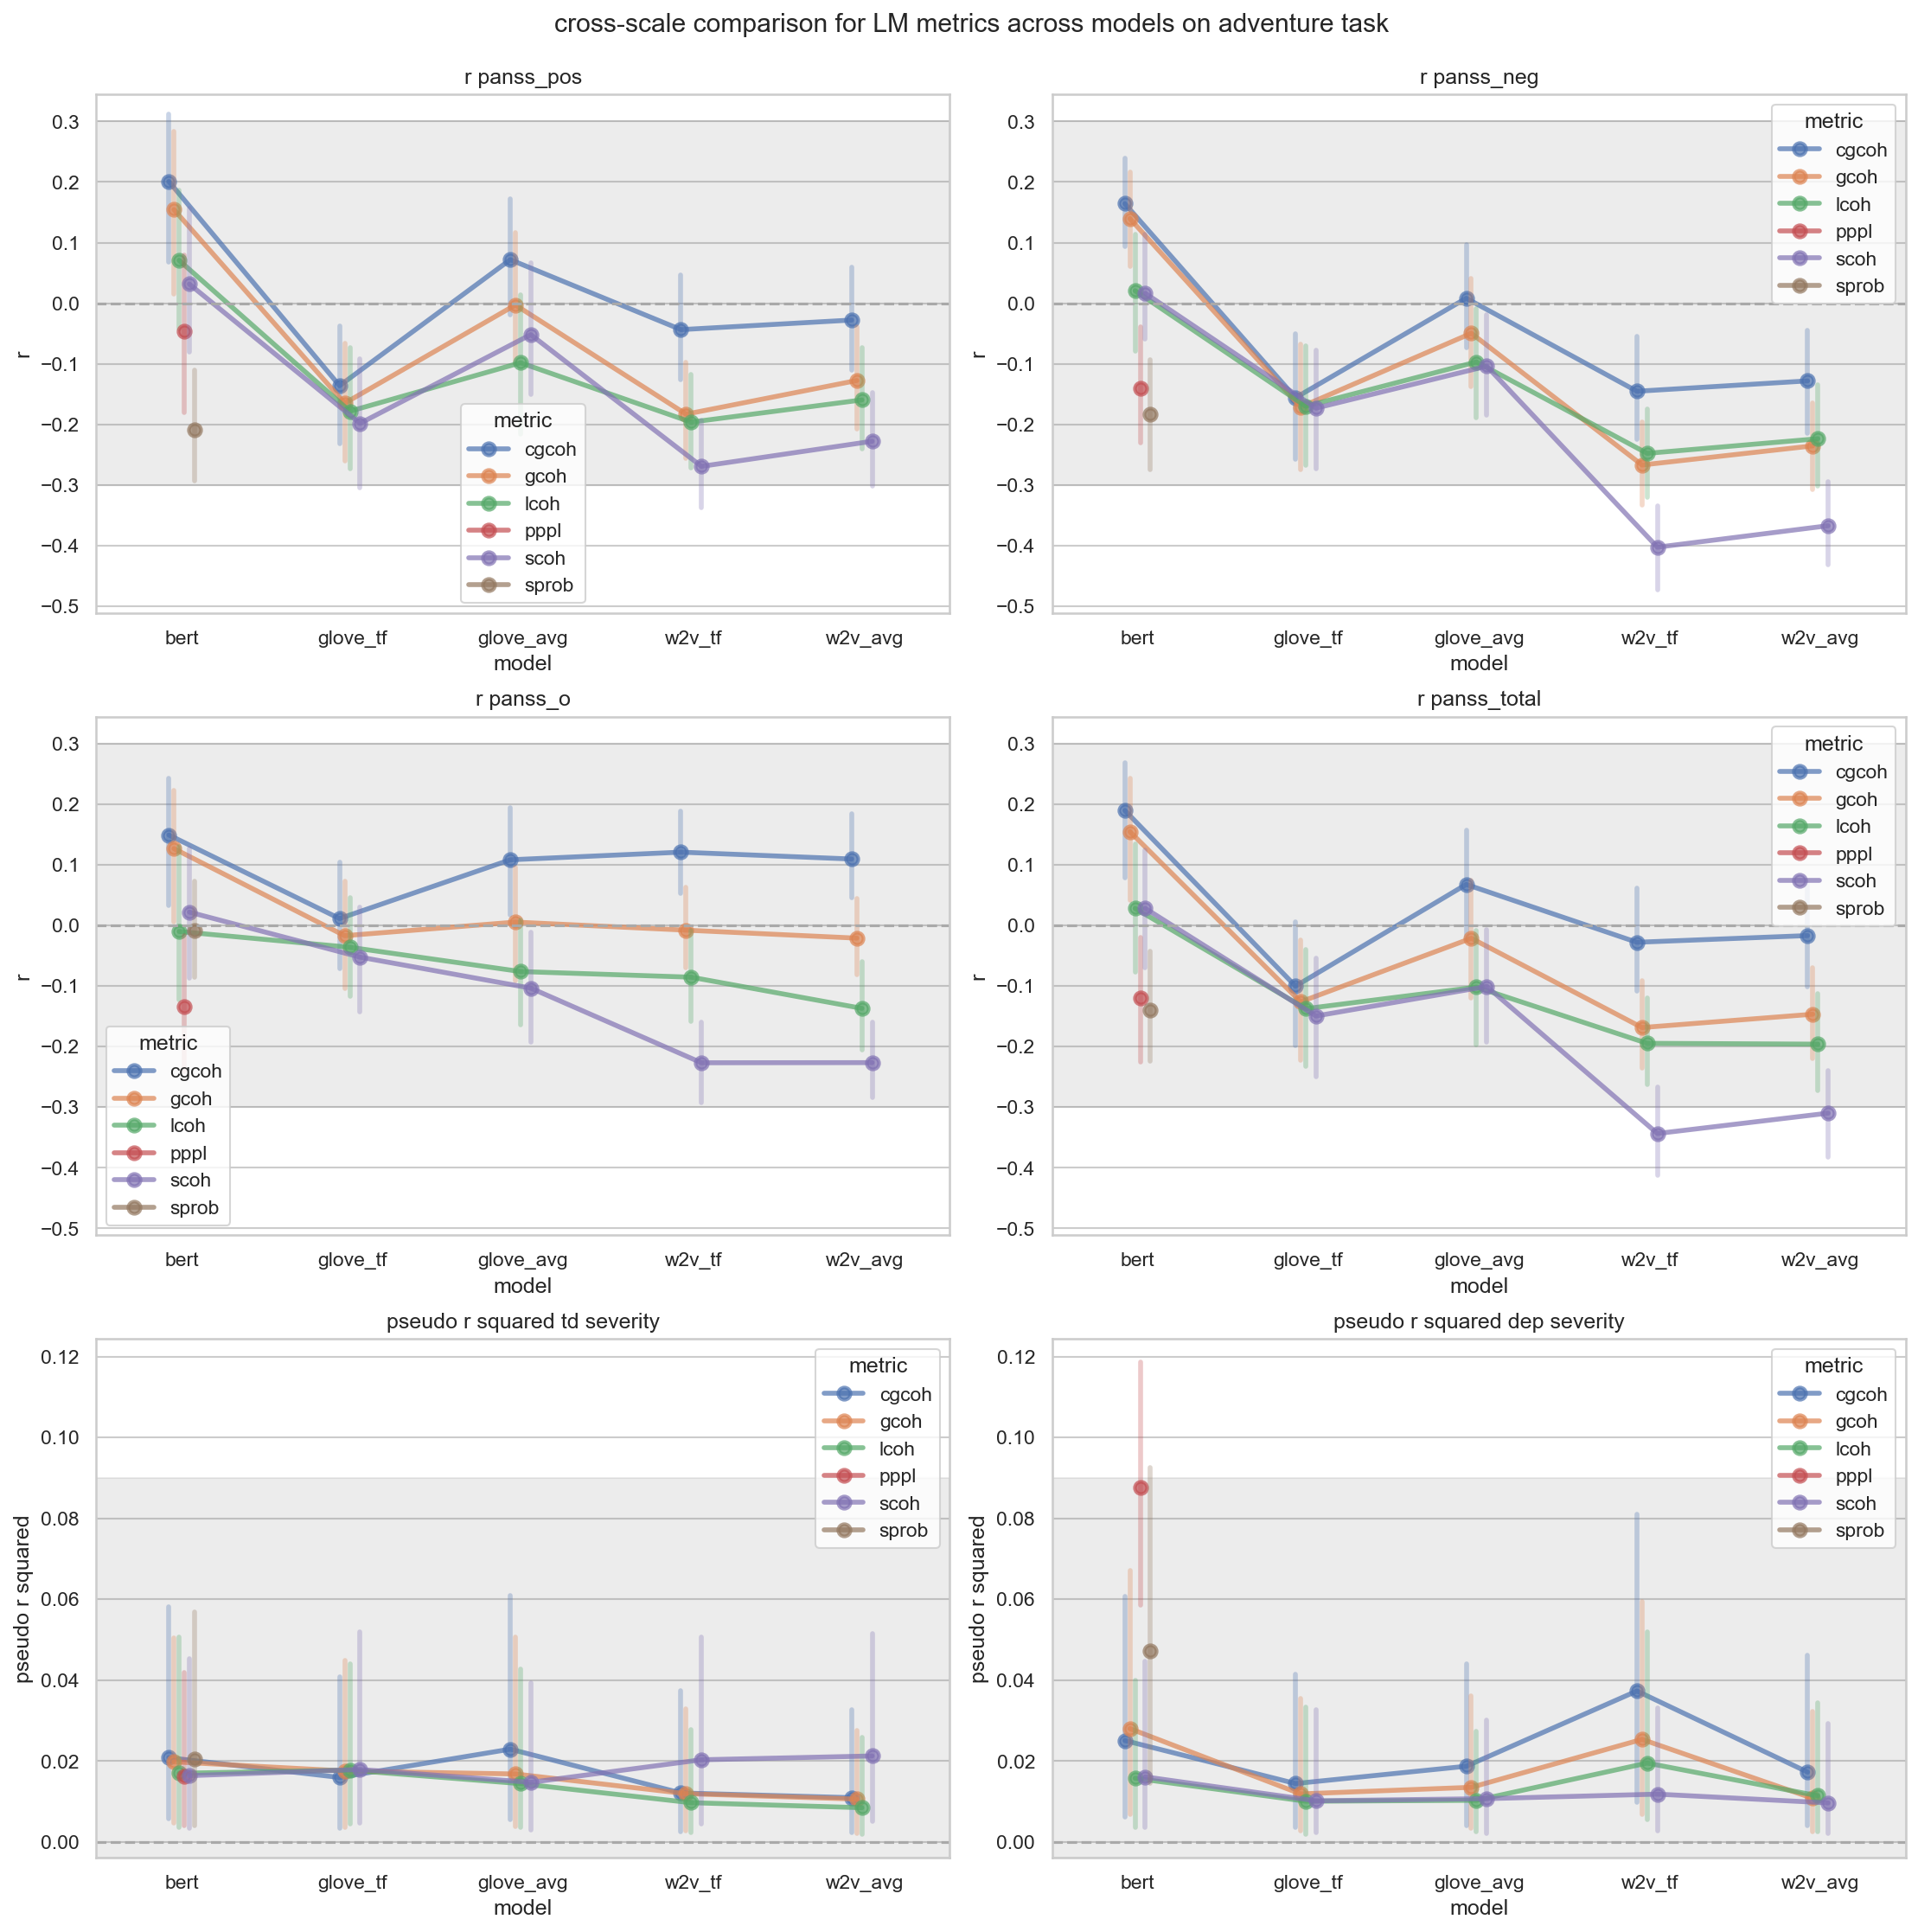
\includegraphics[width=1.1\textwidth, center]{Figures/chapter_4/LM/ru_adventure_scale_r.png} 
\captionsetup{width=\textwidth}
\caption[LM Metrics: Russian, Adventure Task]{\label{fig:results:lm:ru:ad} Pearson's r correlation coefficient and pseudo r squared for each scale for the language model-based metrics on the Russian dataset, adventure task. Grey indicates the values below the 0.3 threshold in absolute value or pseudo r squared below 0.09.}
\end{figure}

% hierarchy of metrics
There was only one metric, that interacted with any scales, namely, second-order coherence, which correlated negatively with PANSS negative and total when calculated with either word2vec weighting scheme. For other metrics, even tough they did not reach the threshold, there was a hierarchy in performance, with second-order coherence being followed by next sentence probability and pseudo-perplexity, and then by local coherence and the two global coherence metrics. 
% cgcoh    0.112622
% gcoh     0.119337
% lcoh     0.120814
% pppl     0.144064
% sprob    0.150057
% scoh     0.153954


% hierarchy of models
word2vec, on average, seemed to outperform the other models, with TF-IDF averaging improving the performance compared to simple averaging for both word2vec and GloVe. BERT under-performed on this task, except for the feature-based metrics. Cosine similarity-based metrics calculated using BERT embeddings, unlike those calculated with either non-contextualized embedding model, tended to correlate positively, rather than negatively, with symptom severity.
% glove_avg    0.085626
% bert         0.109769
% glove_tf     0.122346
% w2v_avg      0.148203
% w2v_tf       0.167033


Figure \ref{fig:results:lm:ru:ch} shows the comparative LM-based metric performance across scales, metrics, and models on chair task. 

Only on this task, depression severity could be predicted, and GloVe TF-IDF could predict depression severity with all metrics but cumulative global coherence. Additionally, averaged word2vec cumulative global coherence correlated positively with general symptoms. 

% hierarchy of metrics
Generally, on this task cumulative global coherence correlated most strongly with symptom severity, followed by pseudo-perplexity, while local coherence and second-order coherence performed worse, and the next sentence prediction showed the worst performance. 
% sprob    0.085901
% lcoh     0.118644
% scoh     0.126696
% gcoh     0.138578
% pppl     0.160010
% cgcoh    0.190945

% hierarchy of models
Among the models, there was no clear patter on this task, though GloVe outperformed word2vec, and TF-IDF outperformed simple averaging, with BERT showing middle correlation strength.
% w2v_avg      0.129196
% glove_avg    0.133443
% bert         0.137969
% w2v_tf       0.140056
% glove_tf     0.167498


\begin{figure}[ht!]
    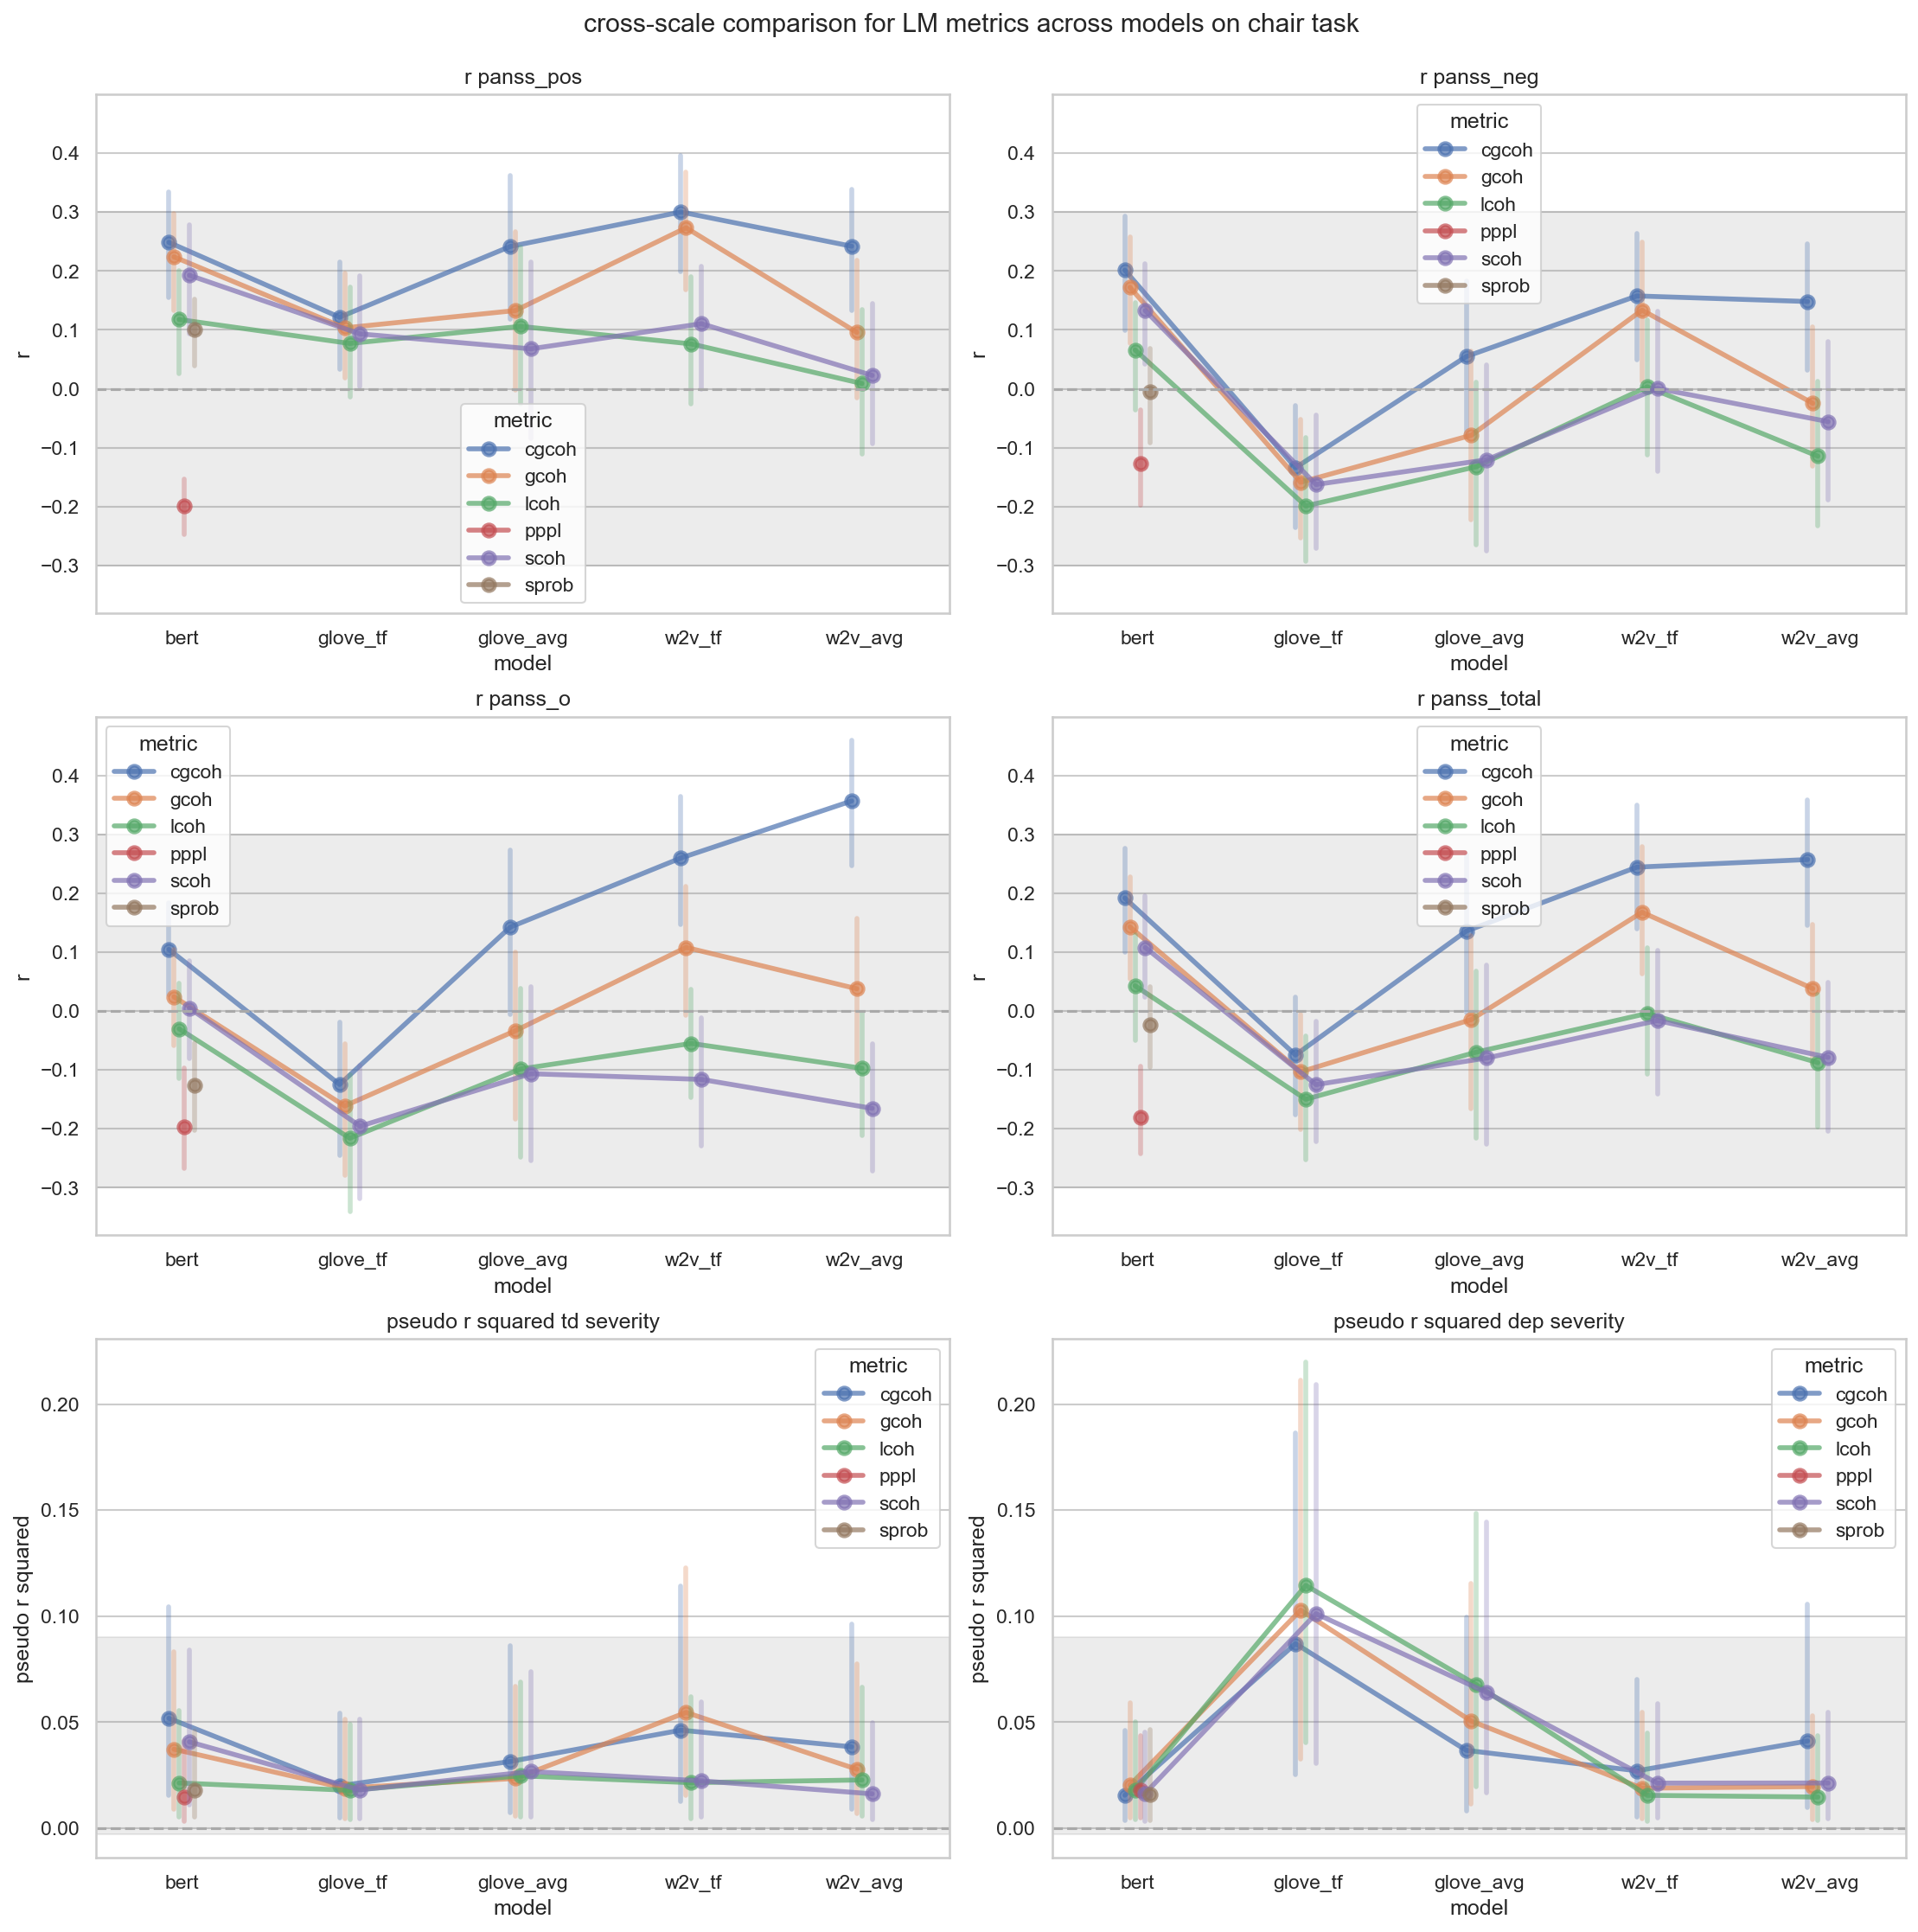
\includegraphics[width=1.1\textwidth, center]{Figures/chapter_4/LM/ru_chair_scale_r.png} 
\captionsetup{width=\textwidth}
\caption[LM Metrics: Russian, Chair Task]{\label{fig:results:lm:ru:ch} Pearson's r correlation coefficient and pseudo r squared for each scale for the language model-based metrics on the Russian dataset, chair task. Grey indicates the values below the 0.3 threshold in absolute value or pseudo r squared below 0.09.}
\end{figure}

\clearpage
Figure \ref{fig:results:lm:ru:pr} shows the comparative LM-based metric performance across scales, metrics, and models on present task. 

\begin{figure}[ht!]
    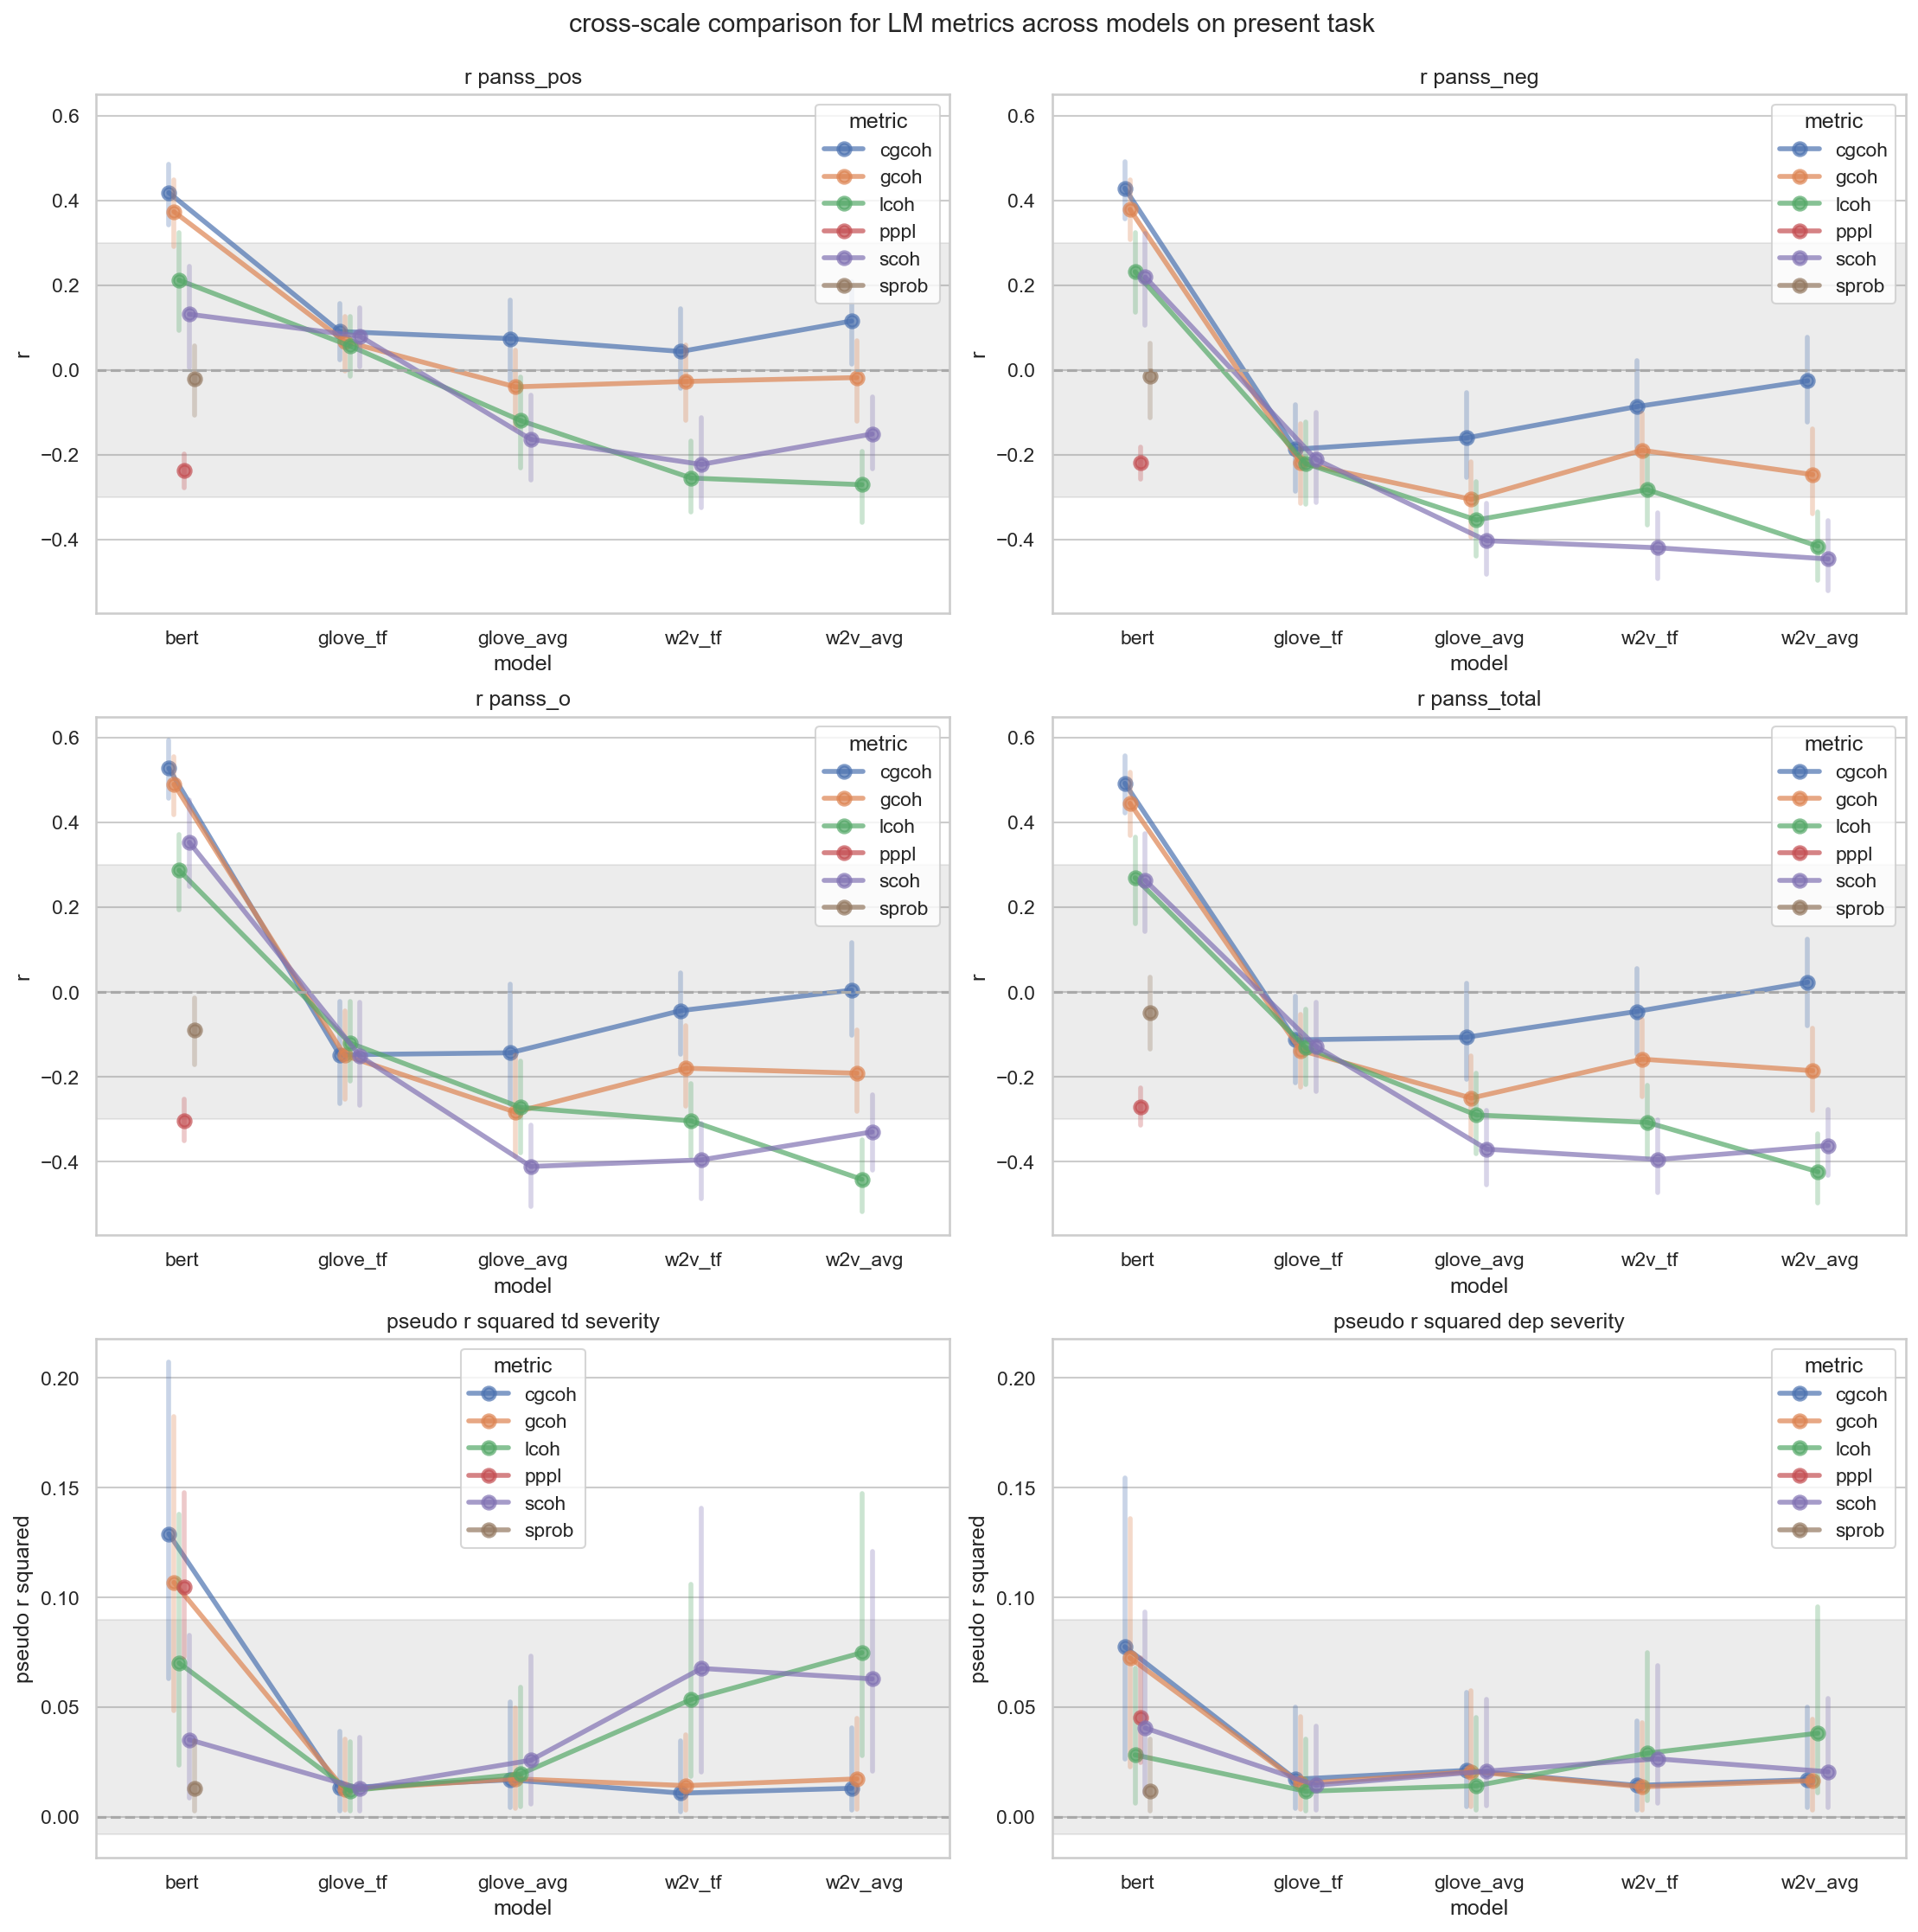
\includegraphics[width=1.1\textwidth, center]{Figures/chapter_4/LM/ru_present_scale_r.png} 
\captionsetup{width=\textwidth}
\caption[LM Metrics: Russian, Present Task]{\label{fig:results:lm:ru:pr} Pearson's r correlation coefficient and pseudo r squared for each scale for the language model-based metrics on the Russian dataset, present task. Grey indicates the values below the 0.3 threshold in absolute value or pseudo r squared below 0.09.}
\end{figure}

On present task, BERT global and cumulative global coherence correlated positively with all scales, while pseudo-perplexity correlated negatively with general symptoms, and they were all predictive of TD severity. Second-order coherence calculated using word2vec with either averaging or GloVe with simple averaging correlated negatively with all PANSS subscales but positive. Local coherence calculated using word2vec correlated negatively with PANSS general and total scores, and when calculated using GloVe with simple averaging it correlated negatively with PANSS negative score.

% hierarchy of metrics
Pseudo-perplexity showed comparatively good performance on this task. When assessed across all models, second-order and local coherence performed best, while global and cumulative global coherence showed worse performance, and next sentence probability barely differed from zero. 
% sprob    0.065762
% cgcoh    0.169817
% gcoh     0.202854
% lcoh     0.237155
% scoh     0.246707
% pppl     0.261305

% hierarchy of models
On this task, as BERT global coherence scores correlated positively with all scales, it showed the best performance of all models. As for the non-contextualized embeddings, word2vec outperformed GloVe, and simple averaging outperformed TF-IDF in absolute correlation strength.
% glove_tf     0.131017
% w2v_tf       0.195729
% glove_avg    0.202681
% w2v_avg      0.211592
% bert         0.317885


% \begin{figure}[ht!]
%     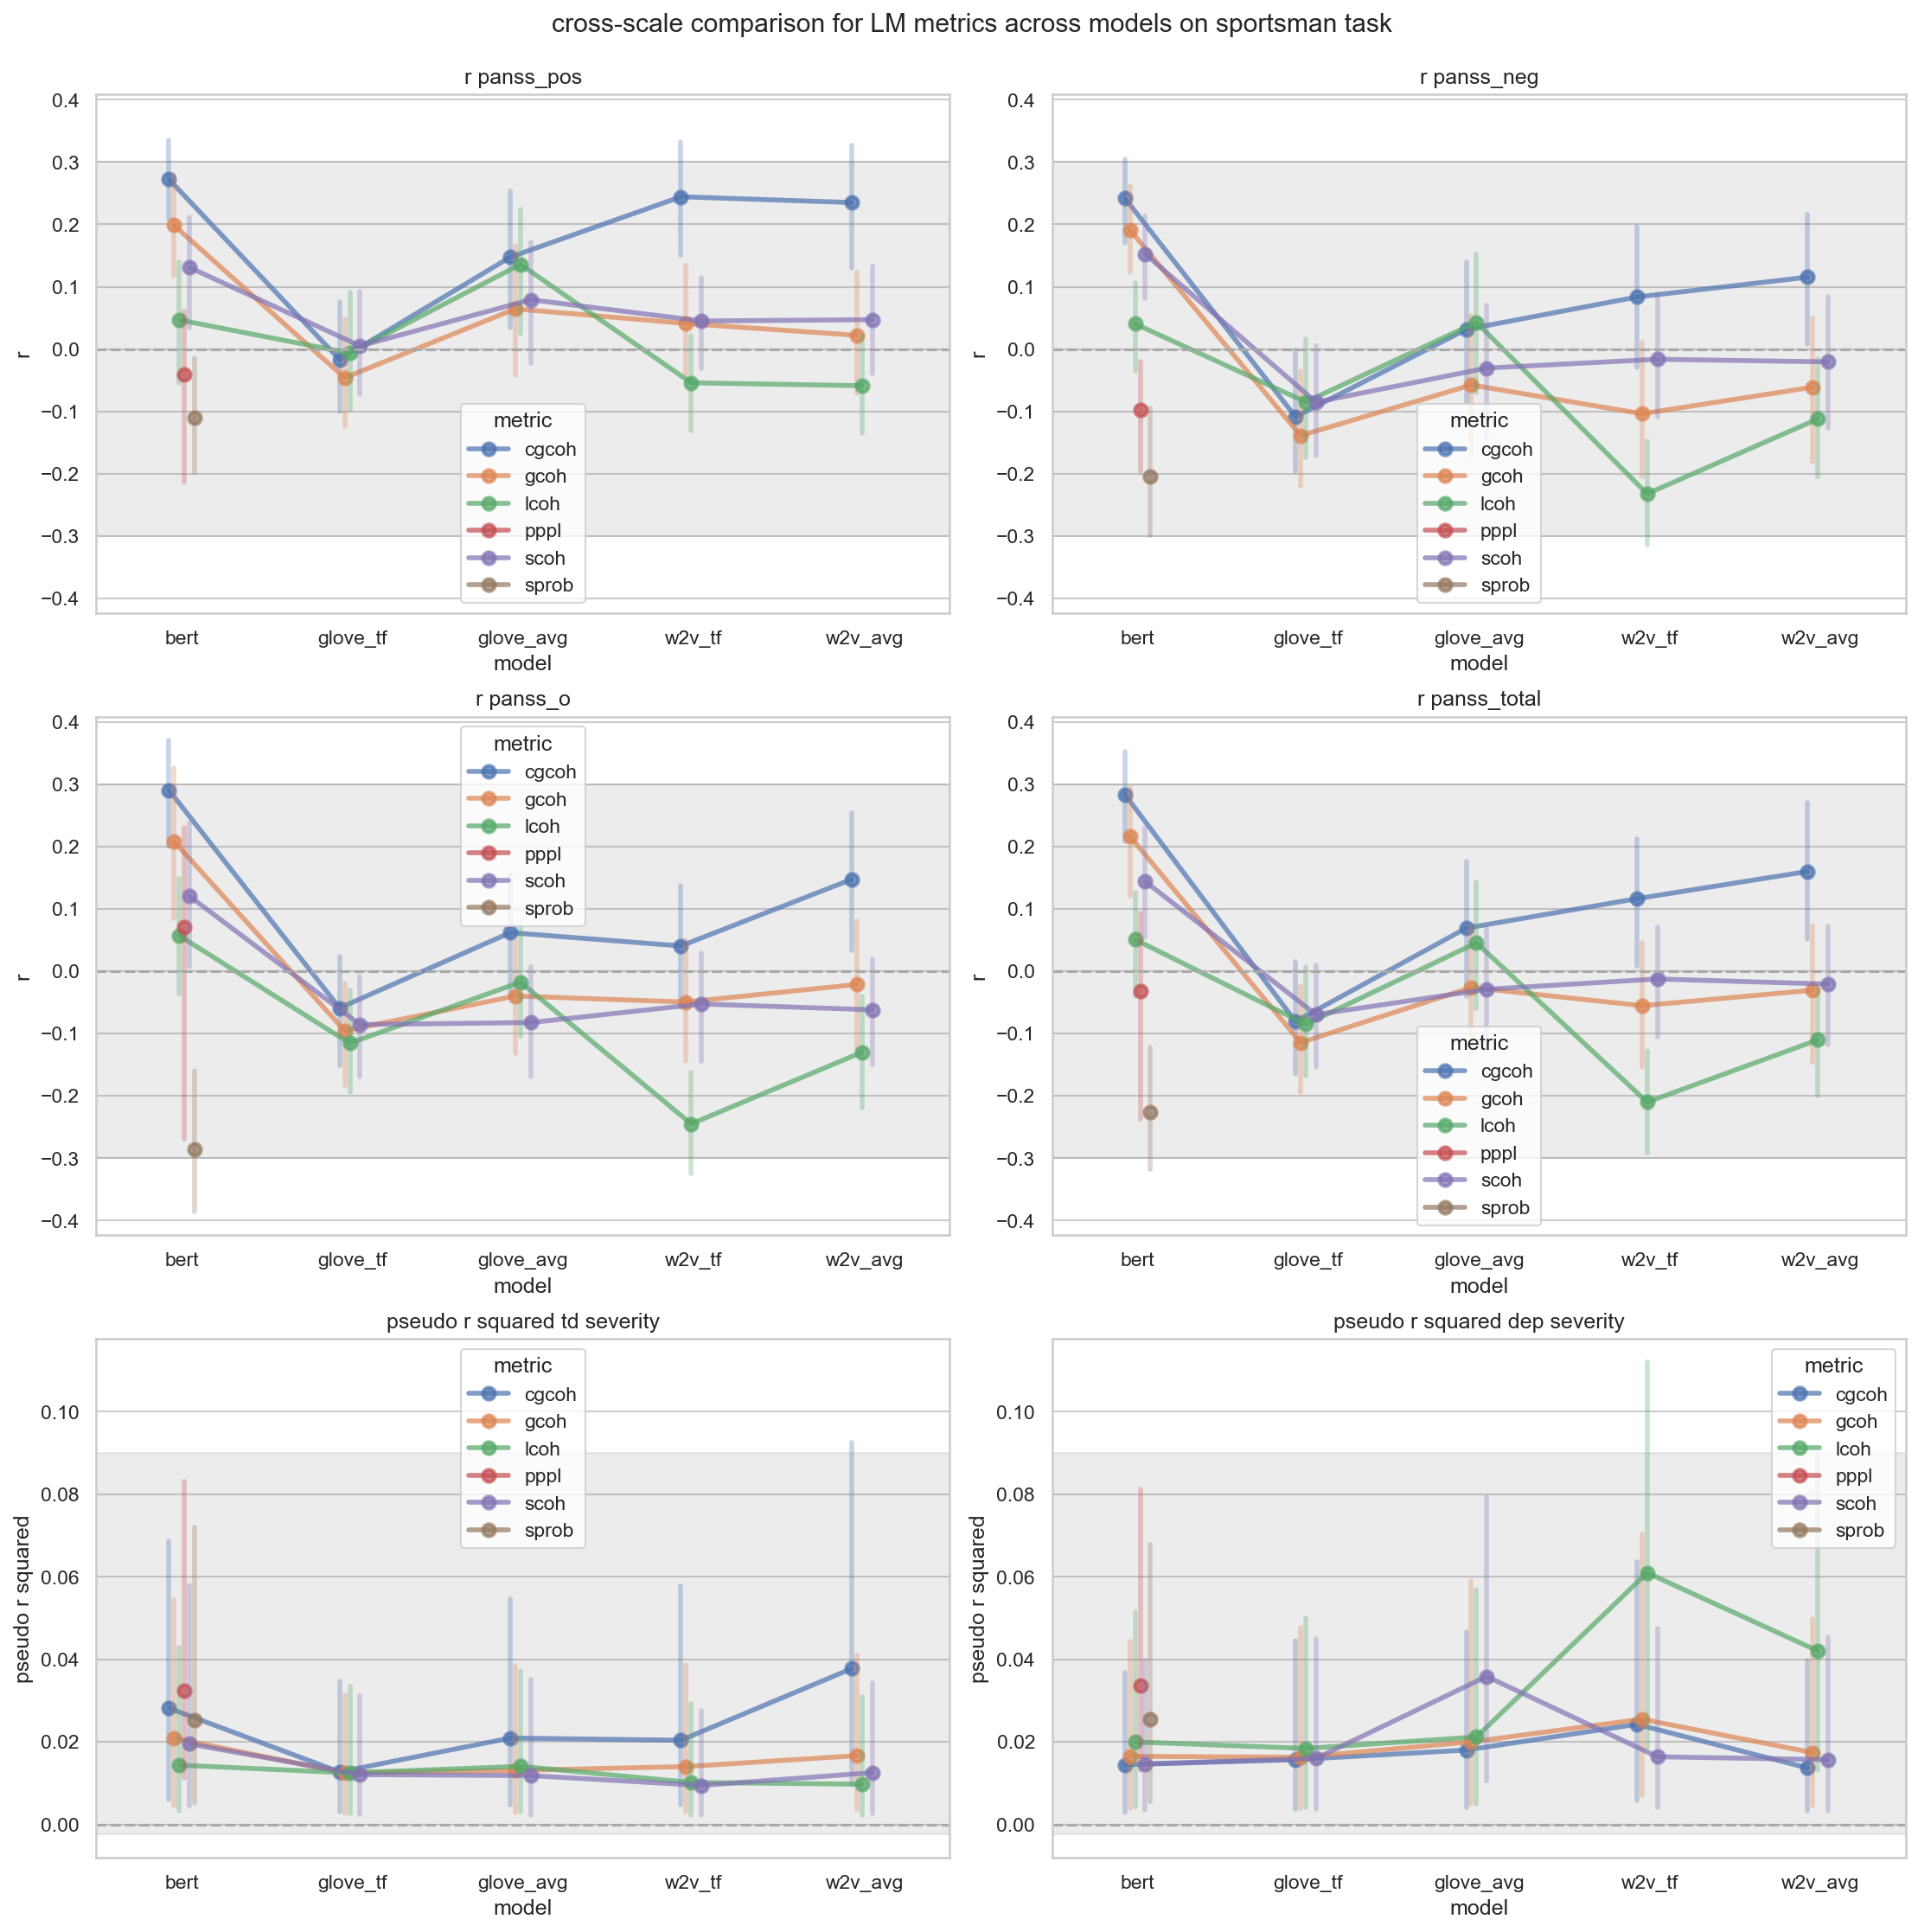
\includegraphics[width=1.1\textwidth, center]{Figures/chapter_4/LM/ru_sportsman_scale_r.png} 
% \captionsetup{width=\textwidth}
% \caption[LM Metrics: Russian, Sportsman Task]{\label{fig:results:lm:ru:sp} Pearson's r correlation coefficient and pseudo r squared for each scale for the language model-based metrics on the Russian dataset, sportsman task. Grey indicates the values below 0.3 threshold in absolute value or pseudo r squared below 0.09.}
% \end{figure}

% sportsman / BERT best model - best but also most difference between the metrics; BERT positive corr(except next sent pred); w2v tf idf no or negative corr; w2v average no corr or positive corr

\begin{figure}[ht!]
    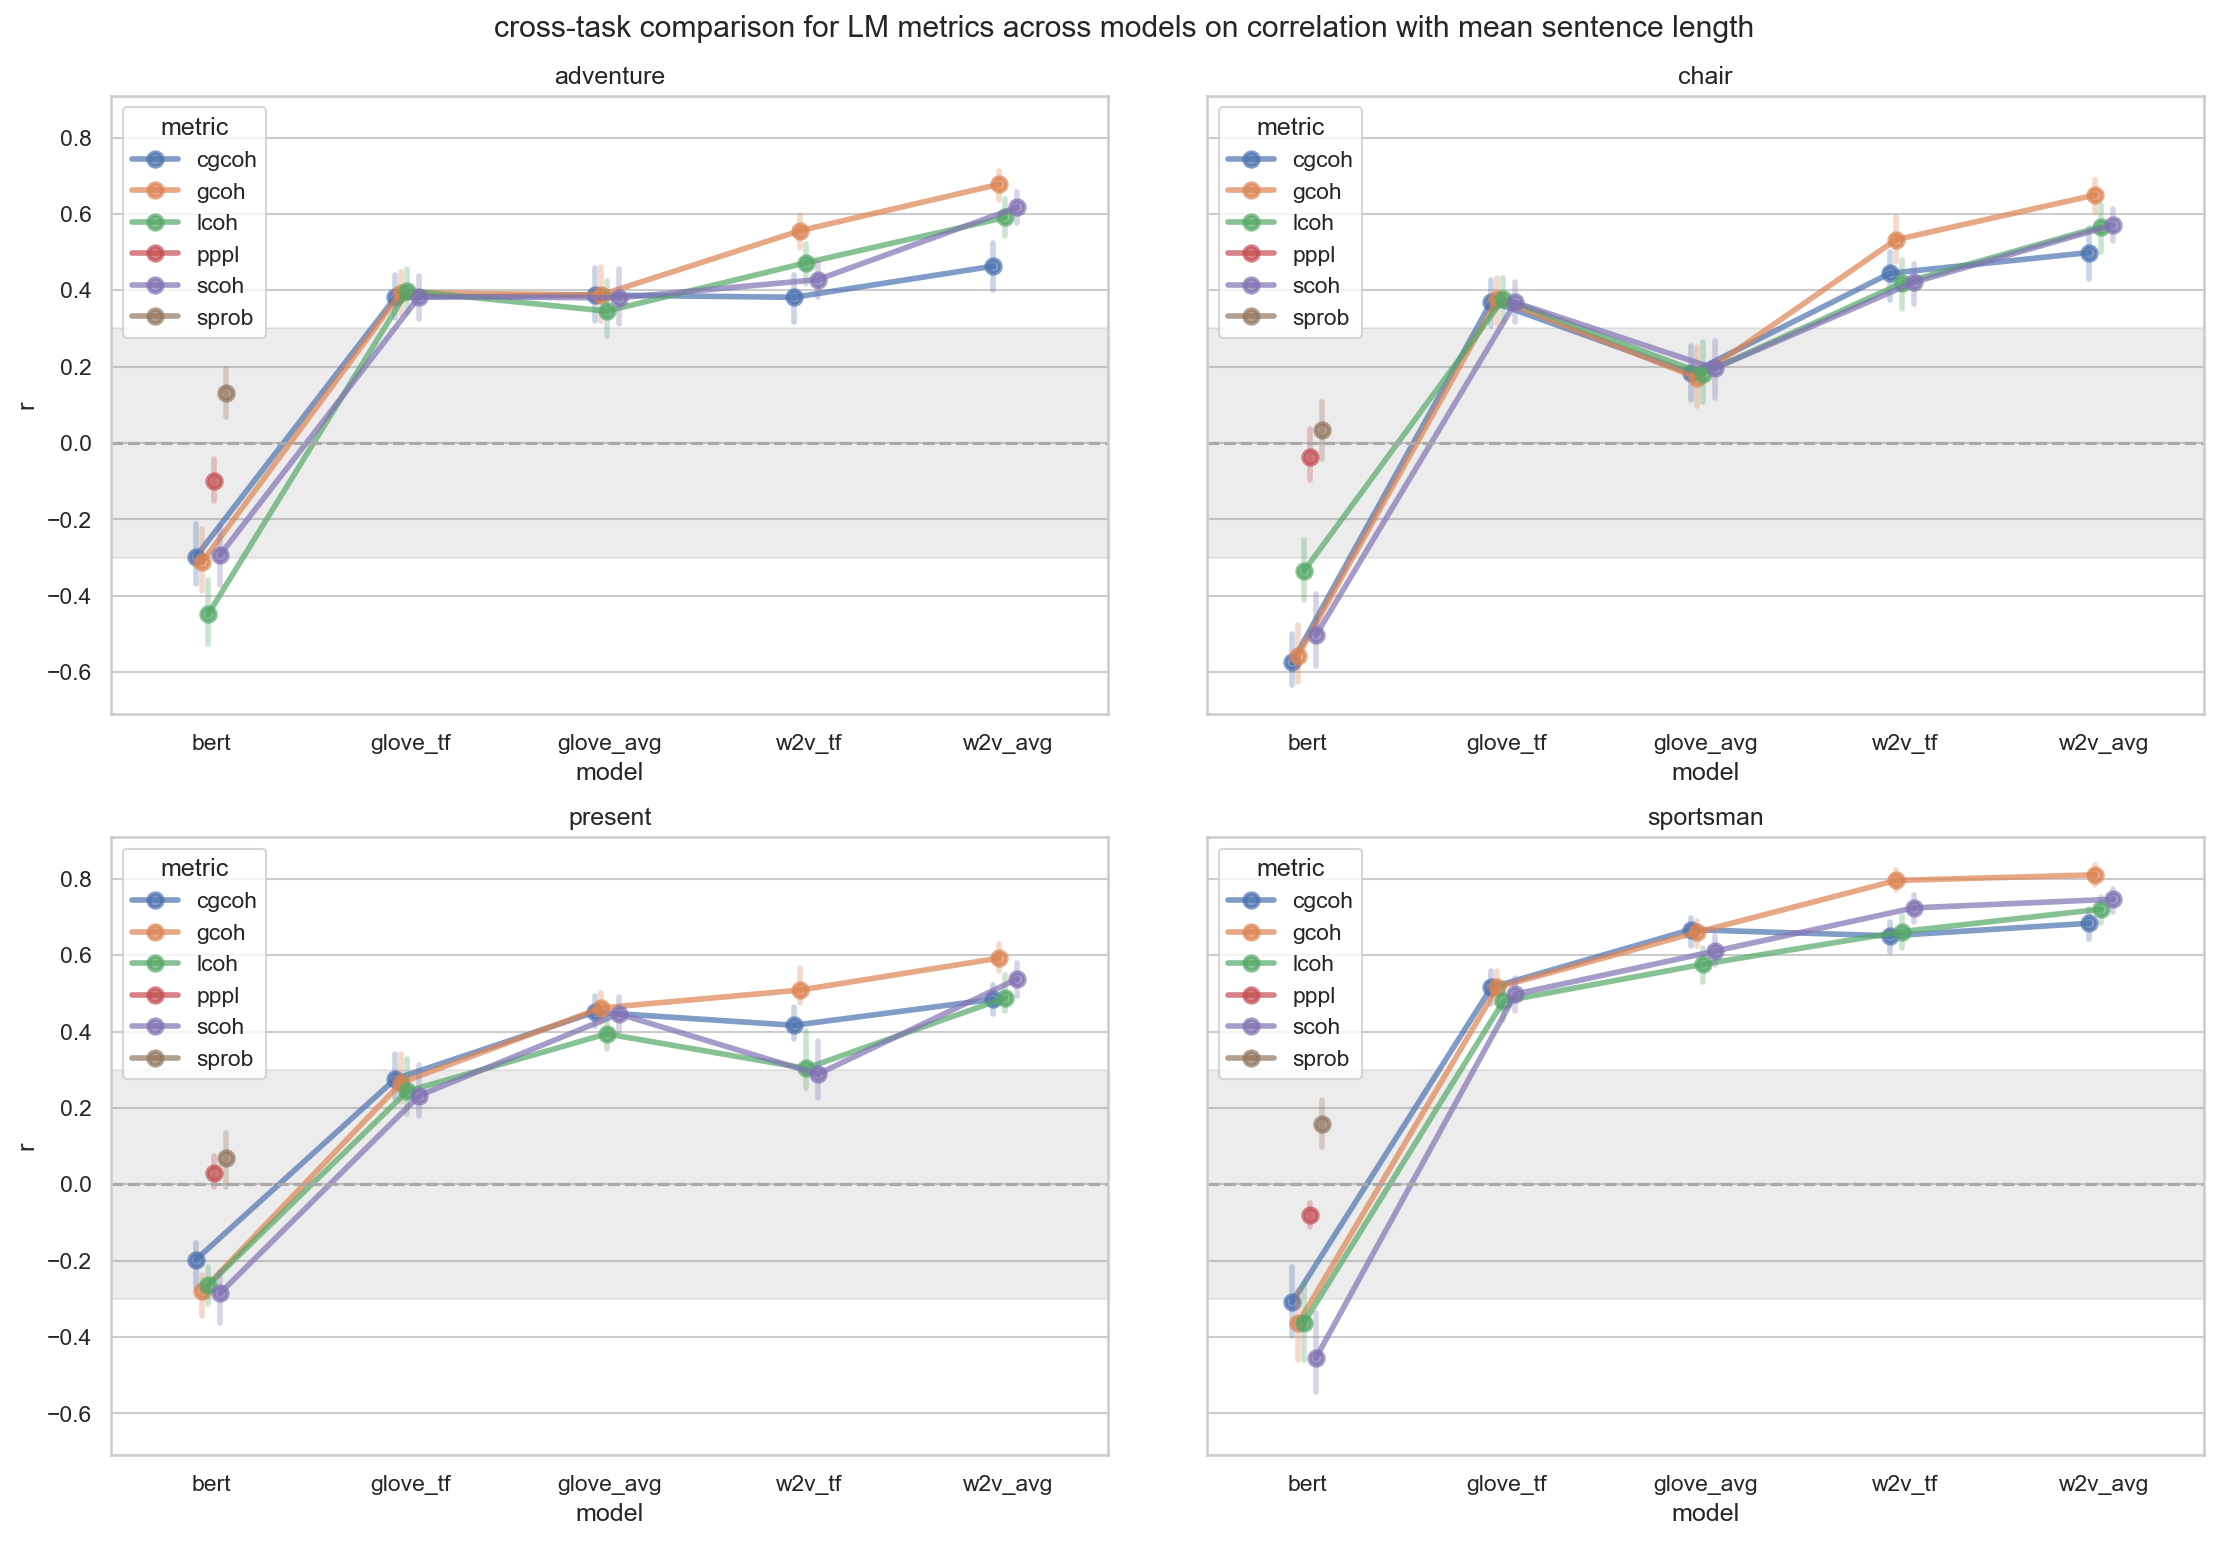
\includegraphics[width=1.1\textwidth, center]{Figures/chapter_4/LM/ru_corr_len.png} 
\captionsetup{width=\textwidth}
\caption[LM Metrics: Russian, Length Correlation]{\label{fig:results:lm:ru:corr_len} Pearson's r correlation coefficient with mean sentence length for the language model-based metrics on the Russian dataset across tasks. Grey indicates the values below 0.3.}
\end{figure}

Figure \ref{fig:results:lm:ru:corr_len} shows the strength of correlation with the mean sentence length across tasks, models, and metrics. 

% corr len
Cosine similarity-based metrics calculated using BERT, correlated negatively with mean sentence length, though the correlation was not equally strong across tasks and metrics, being above the threshold for all metrics on chair and sportsman tasks; only for local and global coherence on the adventure task; and for no metrics on present task. Next sentence probability and pseudo-perplexity did not correlate with length on any of the tasks. 
As for the metrics calculated using GloVe and word2vec, they correlated positively, rather than negatively, with mean sentence length. This correlation was stronger on averaged than on TF-IDF weighed embeddings for all tasks when word2vec was used, and for GloVe it was so on two tasks, sportsman and present, while on chair task the opposite was observed, and almost no difference was seen on the adventure task. All metrics calculated using word2vec correlated with mean sentence length on three tasks and on the fourth, present, second order coherence calculated using TF-IDF averaging did not exceed the threshold. The correlation was above the threshold for all GloVe metrics on sportsman and adventure tasks and was also so for TF-IDF GloVe on chair and for averaged GloVe on present tasks.

Interestingly, across all tasks, cosine similarity-based metrics calculated using BERT showed a positive correlation with the symptom scales and a negative correlation with mean sentence length, while the two non-contextualized embedding models tended to show a negative correlation with the symptoms scales and a positive one with the sentence length. 

There was no clear hierarchy between models or metrics across all tasks, as there was significant interaction between metrics and models, which was also different for different tasks. On average, perplexity, cumulative global coherence, and second-order coherence performed better in absolute correlation strength, while local and global coherence followed closely, and the next sentence probability tended to underperform. BERT and word2vec tended to outperform GloVe, and TF-IDF weighting tended to outperform simple averaging. The performance of word2vec and GloVe seems to be at least partially explained by correlation with mean sentence length.

Across the tasks, there was the same pattern, that cumulative global coherence tended to correlate more positively (or less negatively) than other metrics, and it was followed by global coherence, while local and second-order coherence tended to correlate more negatively. There was, however, a curious difference between the models, as cosine similarity-based metrics calculated using BERT tended also to correlate more positively (or less negatively) than either word2vec or GloVe, which both tended towards a negative correlation. These patterns, when combined, caused a significant model-metric interaction. 

% hierarchy of metrics
% sprob    0.123186
% gcoh     0.140981
% lcoh     0.146947
% scoh     0.153215
% cgcoh    0.153664
% pppl     0.166540

% hierarchy of models
% glove_avg    0.126972
% glove_tf     0.127707
% w2v_avg      0.148330
% w2v_tf       0.154666
% bert         0.180319

\subsection{Cross-Linguistic Comparison}

% German
% hierarchy of metrics (abs)
% cgcoh    0.120598
% gcoh     0.181313
% sprob    0.248705
% lcoh     0.295024
% scoh     0.311049
% pppl     0.340907

% corr len metrics (abs)
% cgcoh    0.284133
% gcoh     0.489777
% lcoh     0.549403
% scoh      0.55498
% sprob     0.57879
% pppl     0.536772

% hierarchy of models (abs)
% bert         0.176137
% glove_tf     0.193866
% glove_avg    0.212054
% w2v_avg      0.263709
% w2v_tf       0.289213

% corr len models (abs)
% bert         0.164279
% glove_tf     0.423349
% glove_avg    0.559389
% w2v_tf       0.588787
% w2v_avg      0.612061

% Russian
% hierarchy of metrics avg acorss tasks (abs)
% sprob    0.123186
% gcoh     0.140981
% lcoh     0.146947
% scoh     0.153215
% cgcoh    0.153664
% pppl     0.166540

% corr len metrics avg acorss tasks (abs)
% pppl     0.060895
% sprob    0.098309
% lcoh     0.431396
% cgcoh    0.431562
% scoh     0.449136
% gcoh     0.493385

% hierarchy of models  avg acorss tasks (abs)
% glove_avg    0.126972
% glove_tf     0.127707
% w2v_avg      0.148330
% w2v_tf       0.154666
% bert         0.180319

% corr len models avg acorss tasks (abs)
% bert         0.364786
% glove_tf     0.379823
% glove_avg    0.406061
% w2v_tf       0.500115
% w2v_avg      0.606063

% differences
There was, for LM-based metrics, little similarity between the languages or tasks. Interestingly, even the direction of correlation with symptoms differed between the samples, as BERT metrics tended to correlate positively with symptoms scales on the Russian sample, but negatively on the German one, where there was no difference in correlation direction between BERT and non-contextualized models. Similarly, pseudo-perplexity correlated positively with symptom severity on the German sample, but negatively on the Russian one, and the reverse was true for next sentence probability. Both these metrics correlated with mean sentence length on the German sample, not on the Russian one, where they were the least strongly correlated of all the metrics.

% similarity in direction of metric correlation pattern
There was a similarity in the tendency for more positive (or less negative) correlation for cumulative global and global coherence across the models and for more negative correlation with symptom severity for local and especially second-order coherence, which was present for both languages.

% corr len patterns
On the German sample, there was a much clearer hierarchy of models and metrics,  which was absent from the Russian sample across the tasks, as there were large differences in performance between them. On both samples, BERT correlated least with mean sentence length, though here, also, the direction of correlation differed between the samples, as on the Russian sample BERT-based metrics tended to correlate negatively with mean sentence length. On both samples TF-IDF clearly helped mitigate the correlation with length, yet, on the Russian sample, this pattern was somewhat weaker and task-dependent. Cumulative global coherence was clearly the least length-dependent for the German sample, but this pattern, if at all present, was also much weaker on the Russian sample. The relative performance of GloVe and word2vec, the latter outperforming the former, seems to be inversely related to the strength of their respective correlation with mean sentence length.

%-----------------------------------
%	section 8
%-----------------------------------
\clearpage
\section{Cross-Group Metric Comparison}
\label{sec:results:clinical:cross_group}

This section compares the performance of the metrics across metric types taking into account only the metrics that showed good performance, comprehending t-test error bars not intersecting zero, above threshold correlation with any of the scales, or above threshold predictive power. Additionally, metrics that were correlated with mean sentence length and performed worse than this baseline on all scales were excluded.

\subsection{German}

Figure \ref{fig:results:comp:de} compares the performance of the metrics across metric groups for all the psychiatric scales on the German sample. Among the metrics that performed well independently of sentence length, was BERT second-order coherence, which correlated negatively with the negative symptoms as well as general and total PANSS scores, and the same correlation pattern was also apparent for the rate of CCONJ. The only other length-independent metric was the AUX rate which correlated negatively with total SAPS score. 

Mean sentence length could only serve as a moderate baseline on the negative scales and PANSS total score. The rate of PART was correlated with length but consistently outperformed this baseline, and correlated positively with all the scales but PANSS positive. Four graph metrics, LCC, LSC, N, and E correlated with length but consistently outperformed it, negatively correlating with all but the two positive symptom scales. LTR showed weak positive correlation patterns, as it only outperformed mean sentence length on general PANSS, and for negative MALTR correlation, the only such scale was total SAPS score. 

\begin{figure}[ht!]
    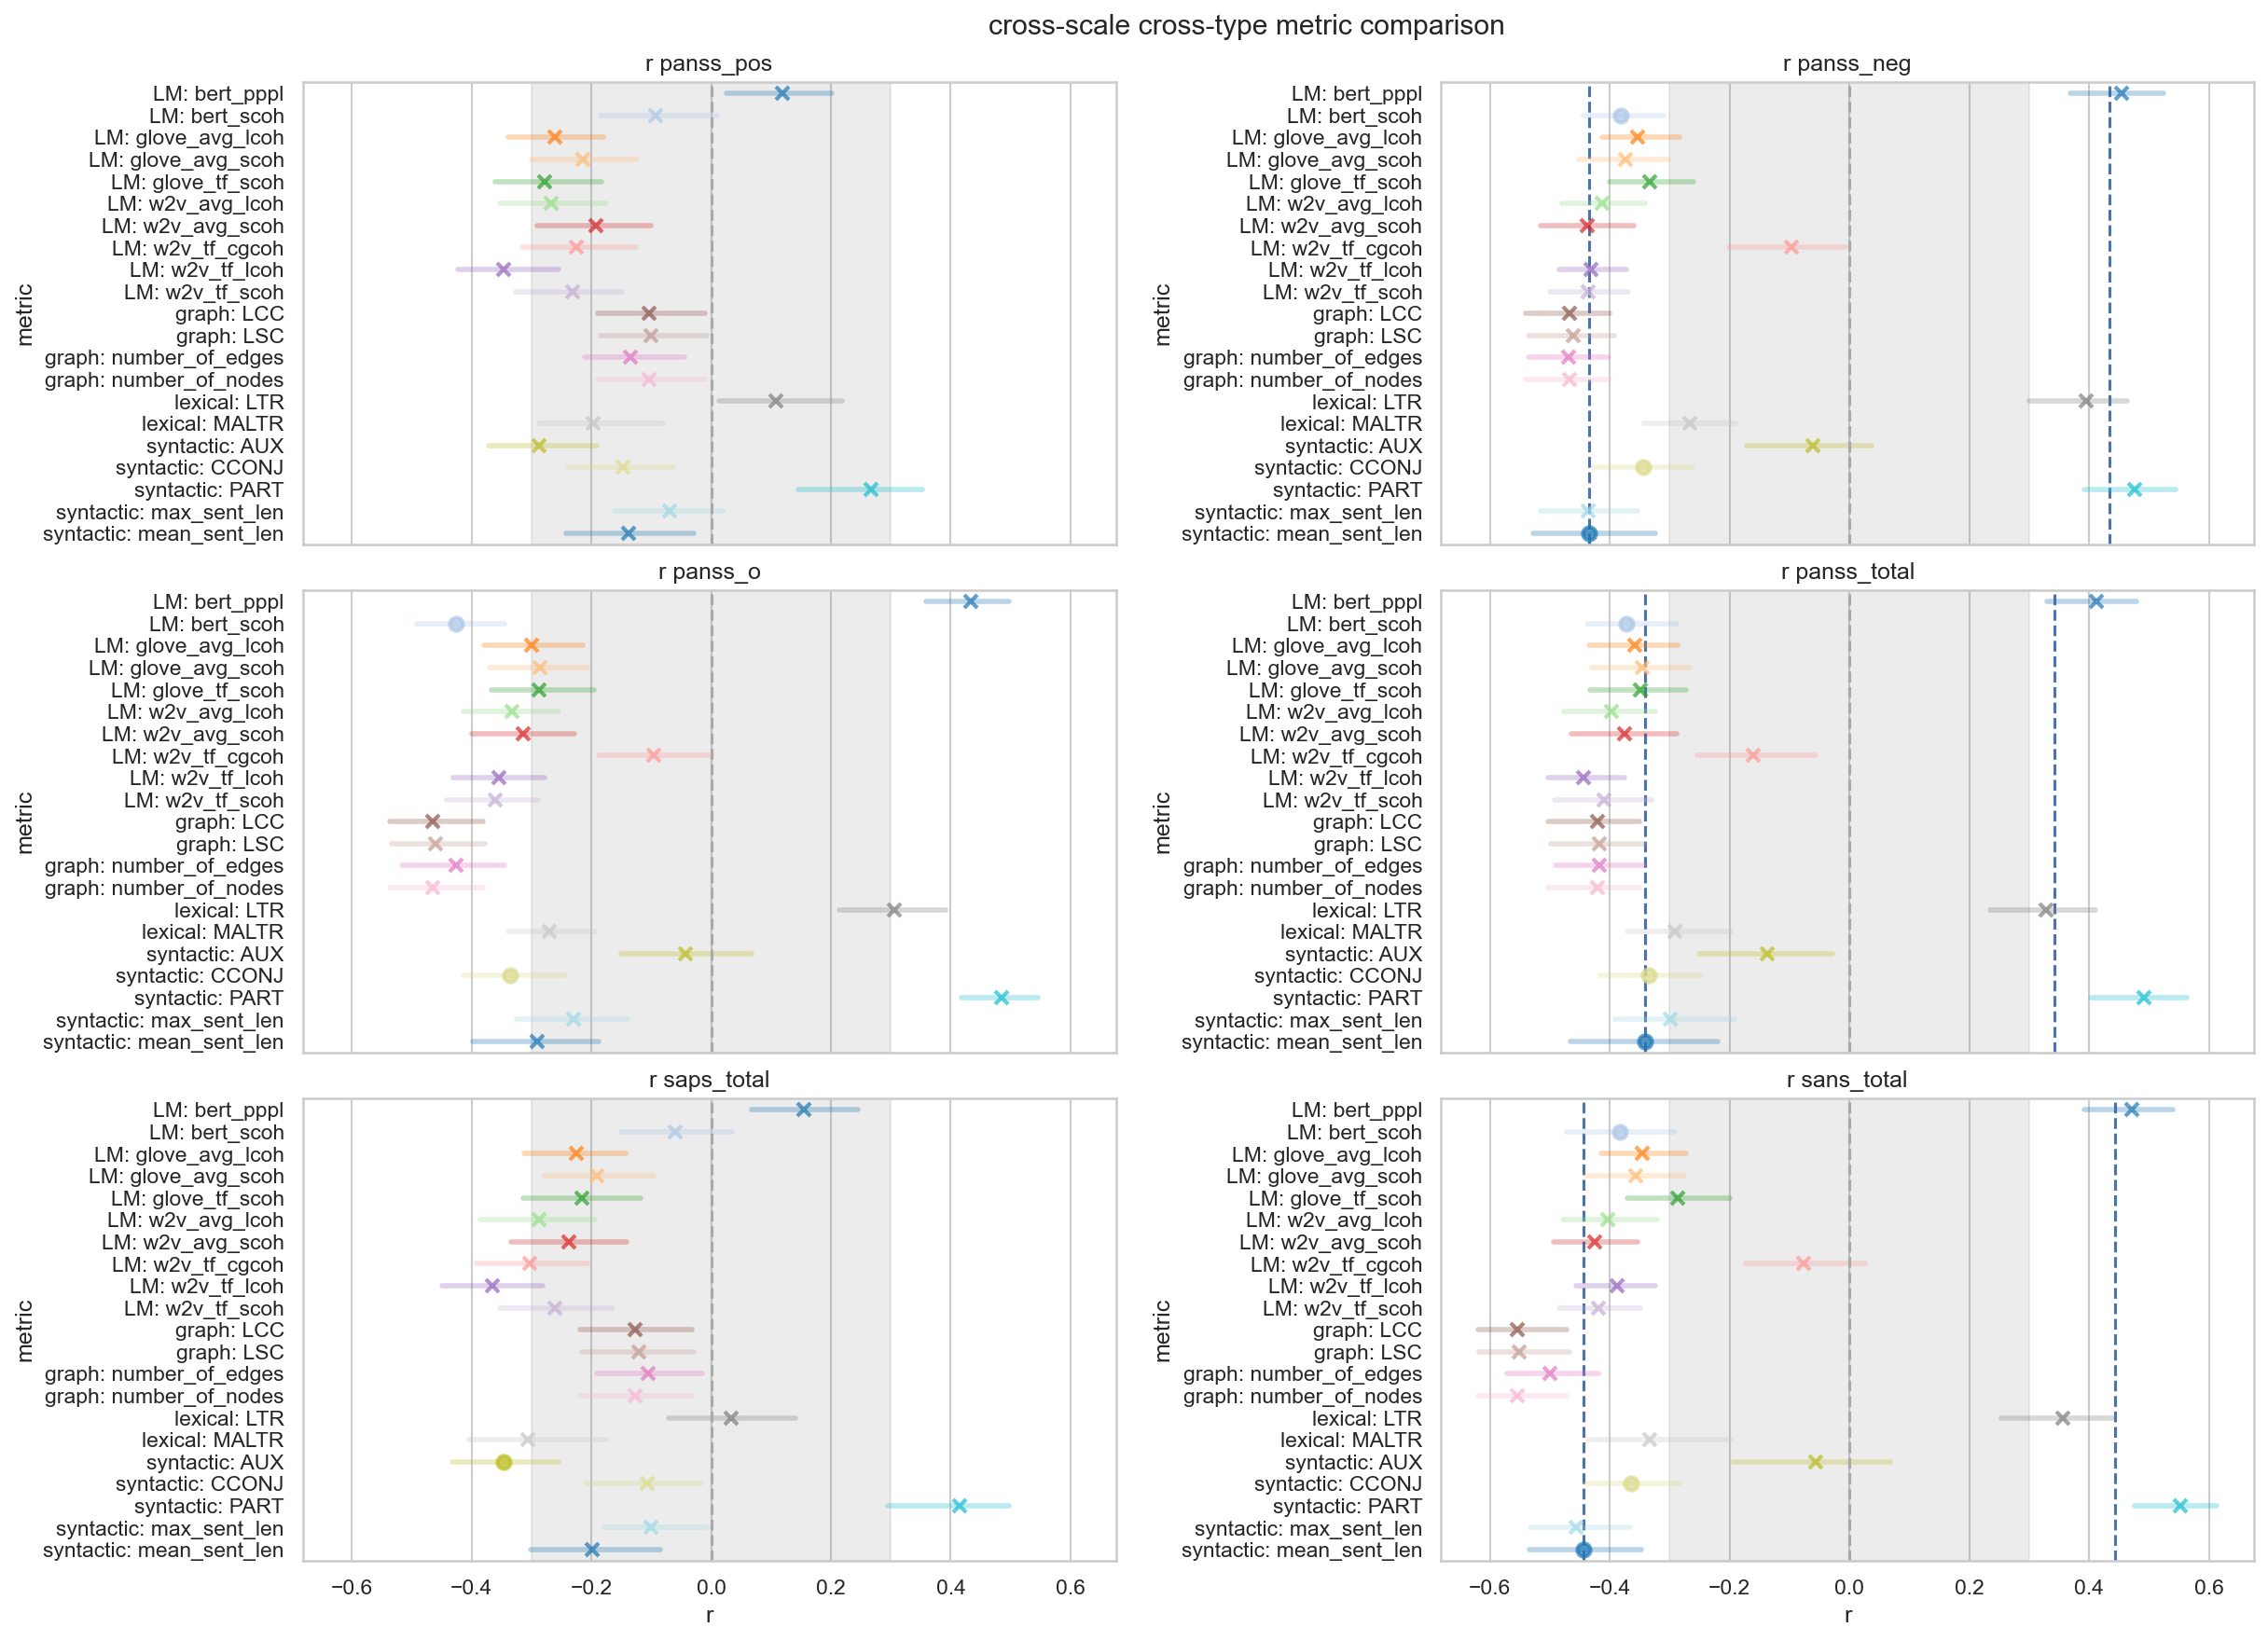
\includegraphics[width=1.1\textwidth, center]{Figures/chapter_4/compare/de_compare_r.png} 
\captionsetup{width=\textwidth}
\caption[Metric Comparison: German, Psychiatric Scales]{\label{fig:results:comp:de} Pearson's r correlation coefficient with each scale across well-performing metrics on the German dataset. Grey indicates the values below the 0.3 threshold in absolute value. The crossed dots indicate the metrics indicate either above-threshold correlation with mean sentence length or below-threshold correlation on a given scale. The mean sentence length baseline is shown by blue dashed line on the scales where this metric serves as a baseline. }
\end{figure}

BERT pseudo-perplexity score correlated more strongly than the mean sentence length baseline with negative and general symptom scales. BERT second-order coherence was uncorrelated with mean sentence length, and performed below the baseline on PANSS negative, but above it on SANS and PANS general and total scores. Averaged GloVe local coherence, which was correlated with length, barely correlated with general PANSS scale and was barely above mean sentence length in the negative correlation with PANSS total score. Averaged GloVe second-order coherence was similarly barely above mean sentence length on the negative correlation with PANSS total score. As for word2vec, all the metrics calculated using it correlated with mean sentence length, but frequently outperformed it, with TF-IDF weighted local coherence correlating with positive symptoms scales and outperforming length on the total PANSS score. Second-order coherence on TF-IDF weighted word2vec was weaker, outperforming the baseline only for PANSS general. Averaged local and second-order coherence calculated with word2vec were barely above the threshold and baseline for PANSS general and total. On the negative scales, where mean sentence length served as a reasonable baseline, all GloVe metrics were below it, while word2vec TF-IDF weighted and simply averaged second-order coherence barely outperformed the baseline for PANSS negative. Maximum sentence length barely outperformed mean sentence length on SANS total but on no other scale.

As negative symptoms predominated in the German sample, it was unsurprising that the performance was overall better on the negative and general symptom scales, with the only exception of the AUX rate. As could be expected, more pronounced patterns could be seen on SANS and SAPS than on the corresponding PANSS subscales. Overall, on the German sample, syntactic metrics showed the most promise, taking into account the mean sentence length baseline. Graph-based and lexical metrics seemed to be to some significant extent explaining the same effects as mean sentence length, yet outperformed this baseline in some cases. Finally, LM, except for pseudo-perplexity, was the least reliable group, with weak correlations, barely ever outperforming mean sentence length. 

\begin{figure}[ht!]
    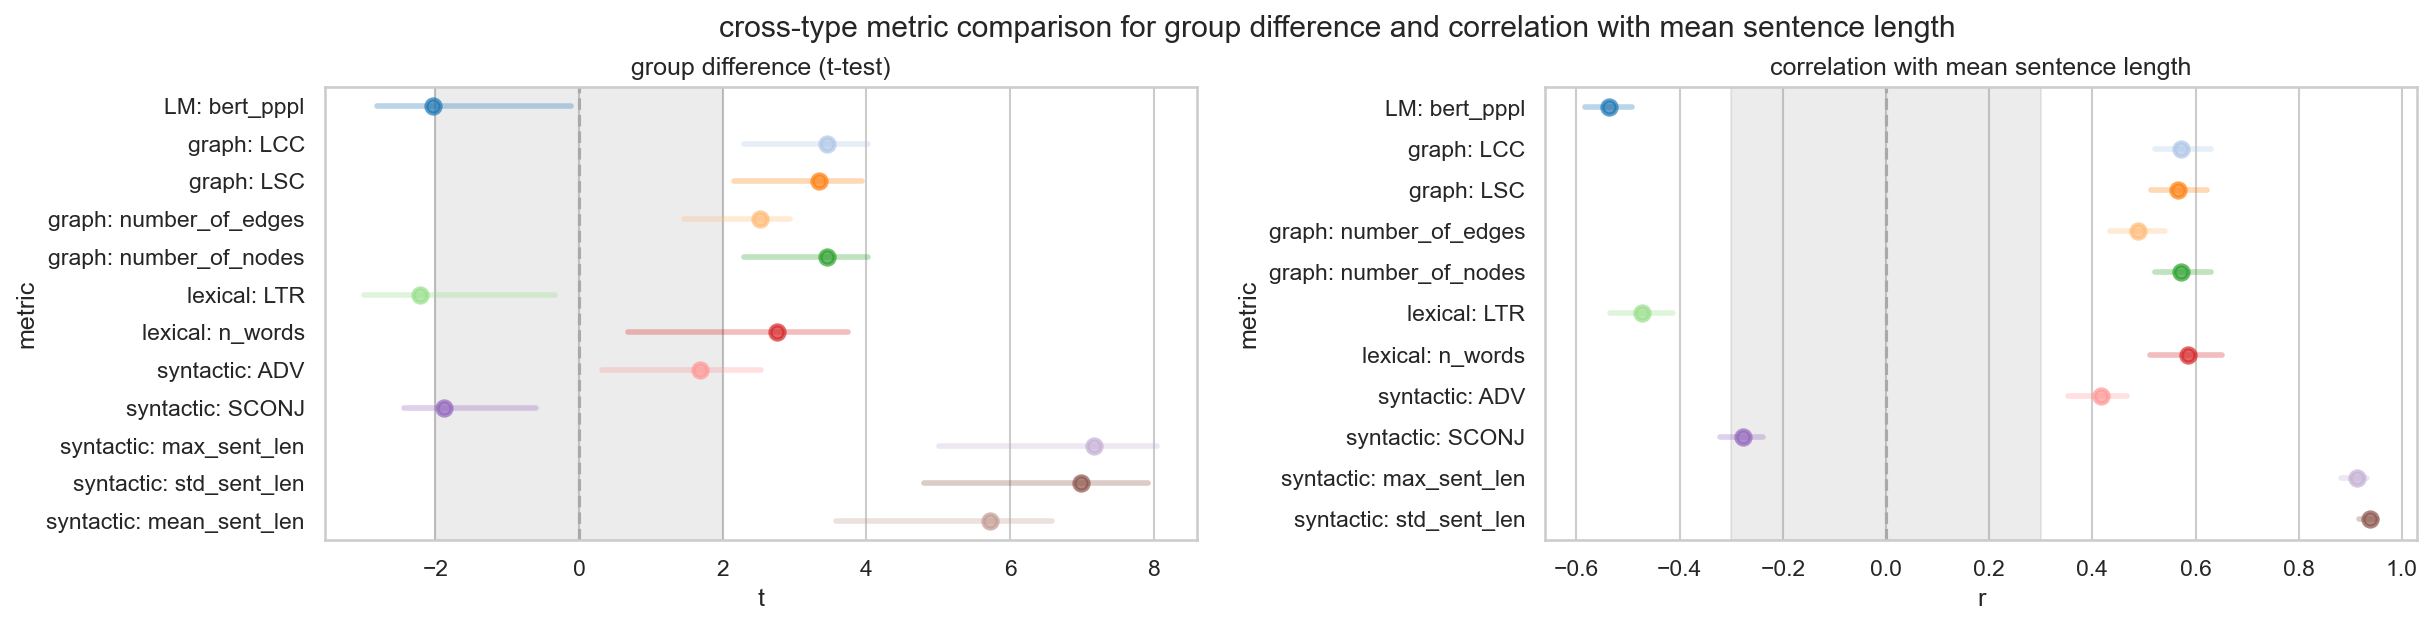
\includegraphics[width=1.1\textwidth, center]{Figures/chapter_4/compare/de_compare_t.png} 
\captionsetup{width=\textwidth}
\caption[Metric Comparison: German, T-Test]{\label{fig:results:comp:de:ttest} T-test and Pearson's r correlation coefficient with mean sentence length for the LM-based metrics on the German dataset. Grey indicates the values below 2 for t score and below the 0.3 threshold in absolute value for correlation coefficient. Only the metrics, for which error bars on T-test do not intersect zero, are shown.}
\end{figure}

Figure \ref{fig:results:comp:de:ttest} compares the t-test effect size to the correlation with mean sentence length for the metrics, the bootstrap 25/75 percentile error bars of which did not intersect zero on the t-test. For all the metrics, the t-test effect size corresponds quite closely with the strength and to the direction of the correlation with mean sentence length. The mean sentence length itself also served as a very strong baseline for the t-test, outperformed, but not significantly so, only by the maximum and standard deviation in mean sentence length. 

\subsection{Russian}

Figure \ref{fig:results:comp:ru} compares the performance of the metrics averaged across tasks for all the psychiatric scales on the Russian sample. The metrics that did not, on average, strongly correlated with length, and performed somewhat well were as follows. The number of words correlated negatively with all PANSS scales and was also predictive of TD severity. LTR, being inversely related to the word count, performed similarly but in the opposite direction, correlating positively with all PANSS scales, yet less strongly than the simple word count. The number of sentences on average correlated negatively with all PANSS scales but positive. Interestingly, the number of parallel edges was on average slightly above the baseline for the positive PANSS subscale.


\begin{figure}[ht!]
    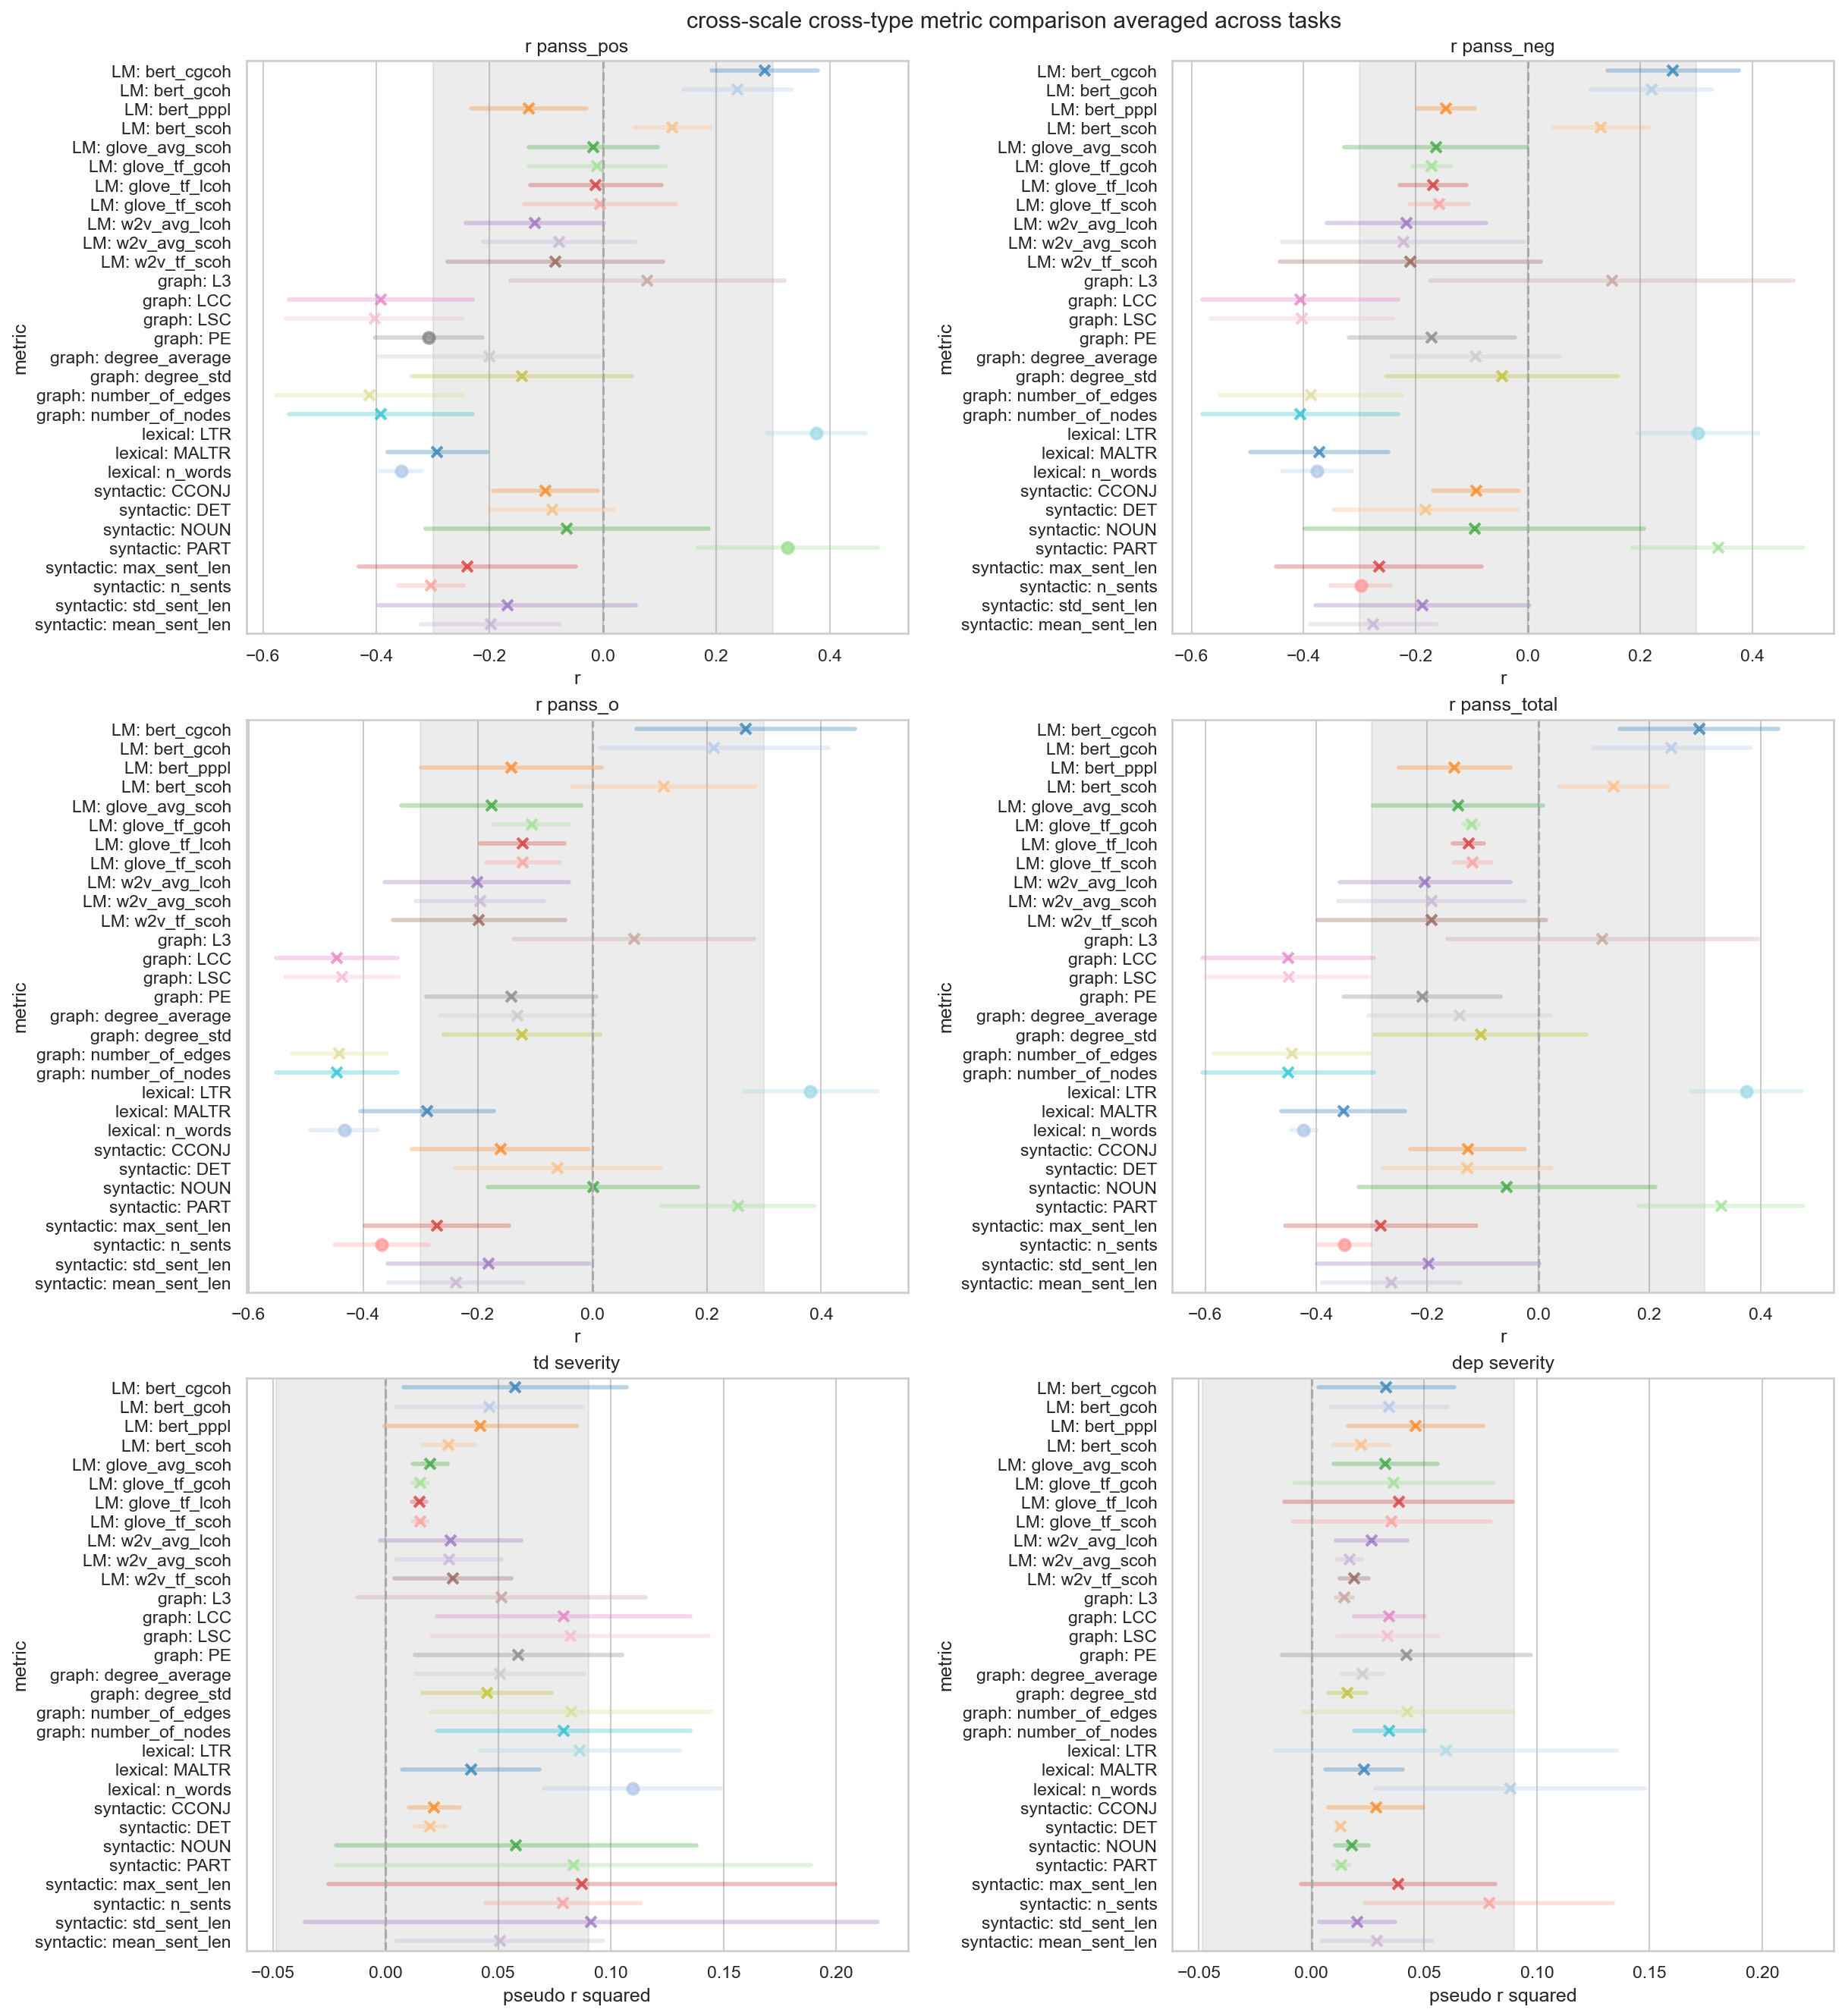
\includegraphics[width=1.1\textwidth, center]{Figures/chapter_4/compare/ru_cross_task_average_compare_r.png} 
\captionsetup{width=\textwidth}
\caption[Metric Comparison: Russian]{\label{fig:results:comp:ru}  Pearson's r correlation coefficient with each scale across well-performing metrics on the Russian dataset, averaged across tasks. Grey indicates the values below the 0.3 threshold in absolute value. The crossed dots indicate the metrics indicate either above-threshold correlation with mean sentence length or below-threshold correlation on a given scale. 
% The mean sentence length baseline is shown by blue dashed line on the scales where this metric serves as a baseline. 
Unlike other plots in this section, the error bars represent standard deviation, and the dot itself is the average value across the four tasks.}
\end{figure}

On the Russian sample, the mean sentence length did not, on average, serve as a reasonable baseline, because the differences were more pronounced in the number of sentences and words, rather than the length of sentences, as discussed above (\ref{sec:results:clinical:sample_length}). LCC, LSC, N, and E consistently outperformed this weak baseline and correlated negatively with all PANSS scales. The rate of PART correlated above baseline for all PANSS scales but the general. The standard deviation in mean sentence length was, on average, barely above the baseline in predicting TD severity. No LM metric was above baseline for any of the scales, when averaged across the four tasks. As depression severity could only be predicted on one task, no metric averaged across tasks, was predictive above baseline, with the number of words and sentences being the strongest predictors. No metric, even on the individual tasks, could differentiate between the groups reliably, as all error bars intersected zero.

\clearpage
Though there were some interactions between the scales and the metrics, the best-performing metrics showed similar results across scales, and the correlation direction was also the same.

On the Russian sample, verbosity was the most robust though not the strongest metric, but otherwise, the tested graph-based metrics outperformed the lexical and syntactic ones, and LM-based ones were by far the weakest.

\subsection{Cross-Linguistic Comparison}
\label{sec:results:clinical:cross_linguistic}

The difference between the languages was about as large as the difference between the tasks on the Russian sample, which, as the tasks were different between the languages, could be the main yet not the only cause for this difference. 

On both samples, LCC, LSC, N, and E were correlated with length, yet outperformed it in the strength of negative correlation with the psychiatric scales. PART rate, on the other hand, was also correlated with length and yet outperformed it in the strength of correlation, correlating positively with the psychiatric scales for both samples. LTR and MALTR correlated with length and were much weaker, sometimes performing worse than the mean sentence length baseline, especially on the German sample, where it was stronger. On the German sample mean sentence length was a stronger baseline than word count or sentence count, while the opposite was true on the Russian sample.

CCONJ rate performed well for the German sample, but weak on average, for the Russian sample. The mean sentence length, due to the differences covered in section \ref{sec:results:clinical:sample_length}, provided a moderate baseline for the German, but not the Russian sample. Instead, on the Russian sample the numbers of words and sentences were much stronger.

Among LM metrics, there was a surprising pattern, as the direction of correlation for BERT metrics was positive on the Russian sample but negative on the German one, and the direction of correlation was inverted for feature-based metrics as well as for cosine similarity-based ones. The perplexity performed well for the German, but not the Russian sample. Across both samples, cumulative global and global coherence correlated more positively with symptom severity than local and second-order coherence, which tended to correlate more negatively. Finally, there was a difference in the strength of correlation with mean sentence length between the languages. However, there was an overall pattern, more evident on the German sample, of BERT being least correlated with sentence length, followed by the TF-IDF and then by simply averaged non-contextualized models, and GloVe being less correlated than word2vec.

In both languages, relatively simple metrics, such as the word count, sentence count, or the number of nodes in the co-occurrence graph, i.e. moving window unique lemma count, showed the best performance, as compared to more complex metrics, such as LM-based ones. Co-occurrence graphs showed a promising result overall, and so did the syntactic metrics, though, the POS rates less so that simple unit length and count. 
% Chapter Template

\chapter{Discussion} % Main chapter title
\label{chap:5:discussion}

This chapter is dedicated to the interpretation of the results described above. The chapter covers each group of methods and compares the results with the ones reported in other studies (\ref{sec:discussion:lexical}-\ref{sec:discussion:LM}). After that, there is a comparison of cross-methodological results (\ref{sec:discussion:cross-method}), a discussion of study limitations (\ref{sec:discussion:limitations}), and a short conclusion (\ref{sec:discussion:conclusion}).

%-----------------------------------
%	section 1
%-----------------------------------
\section{Lexical Methods}
\label{sec:discussion:lexical}

As in other studies in the field, lower overall verbosity was observed on the German sample, though, on the Russian sample, the t-test error bar crossed zero even for this metric. Overall verbosity was also negatively correlated with all PANSS subscales, and, on some tasks, with TD and depression severity, meaning that any severe symptom was associated with a decreased word count for the Russian sample. However, on the German sample, where positive symptoms were less pronounced, lower verbosity was only associated with negative symptom severity. 

With regards to LTR, the results on the German sample are in line with the findings that reported lower TTR in the patient group \citep{willits2018evidence, aich2022towards, minor2023automated}, but, on the Russian sample, there were no meaningful group differences, in line with the results reported by \citet{hitczenko2021understanding, jeong2023exploring, schneider2023syntactic}. The results of the present study contradict the findings reported in \citet{ziv2022morphological}, as LTR was lower, rather than higher, in both samples, despite the gap in the size of this difference. LTR also correlated positively with negative and general scales on both samples and, on the Russian sample, also with positive symptoms, as well as being somewhat predictive of TD and depression severity. The positive correlation could be explained by the inverse proportion to overall verbosity which correlated negatively with symptom severity. This hypothesis is partially confirmed by the fact that the opposite direction of correlation was observed for moving average LTR, for which the effect of overall verbosity is mostly negated. In both samples, simple word count performed better than LTR. The fact that MALTR performed much worse in absolute value than LTR, coupled with the fact that the word count outperforms LTR, also suggests that the most predictive strength of LTR comes from the word count component of this metric.


% TTR lower in the patient group \citep{willits2018evidence, aich2022towards, minor2023automated}, though some report no significant differences \citep{hitczenko2021understanding, jeong2023exploring, schneider2023syntactic}, or higher \textit{type} and \textit{lemma-token ratio} \citep{ziv2022morphological}.

% The lexical methods may aim at capturing both to positive and negative FTD features. Verbosity in penitents may either be increased (pressure of speech) or decreased (poverty of speech). Lexical diversity and density may be increased (paraphasias) or decreased (poverty of speech and content). Sentiment analysis may reveal the blunted affect which is a typical non-linguistic negative symptom of schizophrenia. Finally, topic analysis may reveal common semantic features shared between different patients which may be related to both negative and positive symptoms.


% German
% LTR + p_n p_t p_o sn - T - msl
% MALTR - sm sp + msl
% n words - p_n sn + T + msl

% Russian
% Overall, on the Russian sample, LTR correlated positively across PANSS subscales but for one task, and word count correlated negatively across PANSS subscales but for one task, while MALTR only performs on two tasks. LTR and word count are also predictive of TD severity on two tasks and of depression severity on one task, while not being overly strongly correlated with mean sentence length.
% adventure
% MALTR - p_n, p_o, p_t + msl
% n words - p_n, p_p, p_o, p_t
% chair
% LTR + D, p_n, p_p, p_o, p_t - msl
% MALTR - p_n, p_p, p_o, p_t + msl
% n words - D, p_n, p_p, p_o, p_t + msl
% present
% LTR + TD, p_n, p_p, p_o, p_t
% MALTR - p_n + msl
% n words - TD, p_n, p_p, p_o, p_t 
% sportsman
% LTR  + TD, p_n, p_p, p_o, p_t - msl
% n words - TD, p_n, p_p, p_o, p_t

%-----------------------------------
%	section 2
%-----------------------------------
\section{Syntactic Methods}
\label{sec:discussion:syntactic}

The part-of-speech rates obtained in the present study align only partially with the results reported previously. 

% DET
Even though DET rates were often reported to be lower in the NAP or SDD patients for several languages\footnote{\cite{bedi2015automated, corcoran2018prediction, sarzynska2021detecting, tang2021natural}}, the present study found no group differences in DET rates in either sample, similarly to the results reported for CHR populations \citep{bilgrami2022construct, haas2020linking}. Nevertheless, there were some negative correlations with negative symptom severity on one of the tasks in the Russian sample, contradicting the absence of such association reported by \citet{corcoran2018prediction, bilgrami2022construct} and higher article use reported by \citet{mitchell2015quantifying}.

% PRON
The experiments conducted here could find no effects for pronoun use, contradicting partially the results reported by \citet{corcoran2018prediction, jeong2023exploring}. 
This also does not support the idea that reduced pronoun use could be used to detect poverty of speech typical of negative FTD, as negative symptoms were prevalent in both samples and yet pronoun rates remained unaltered.
% SCONJ CCONJ
Unlike what has been reported \citep{silva2022syntactic}, no effect could be observed for subordinating conjunction (SCONJ) use, but instead, there was a relatively consistent negative correlation with general symptoms for coordinating conjunction use (CCONJ). This could be indicative of lower syntactic complexity and poverty of speech, yet this is not explored in sufficient detail in the present work to make any certain claim.
% ADJ ADV
No differences or correlation with symptom severity was observed for ADJ and ADV rates, contradicting the papers claiming both higher \citep{corcoran2018prediction, tang2021natural, ziv2022morphological} and lower \citep{argolo2023burnishing} rates in patient populations. This result does not support the idea that the reduction in these POS types could consistently indicate the poverty of speech content often present in negative FTD.
% VERB
Similarly, no effects were found for verb rates, in line with the results reported by \citet{tang2021natural, argolo2023burnishing, haas2020linking}, but in contradiction with lower verb rates reported for a Hebrew-speaking population \citep{ziv2022morphological}.

% AUX
Interestingly, AUX rates were associated negatively with positive symptoms on the German sample but not on the Russian one. This is the more surprising as the positive symptoms were less pronounced on the former than on the latter, and this result may have to do with the difference between the languages, rather than the tasks or the populations. The reduction in AUX use could be a marker of lower syntactic complexity, but it is not entirely clear whether it is indicative of it, and if so, why it is associated with positive, rather than negative symptoms.
% NOUN
There was a slight negative correlation of NOUN rates with both positive and negative symptoms on one of the tasks for the Russian sample, yet this result could be explained merely by the positive correlation with mean sentence length.
% PART
Most surprisingly, the best result for POS rates was observed for PART use, which was not reported as a good metric in any of the reviewed studies, yet it correlated positively with all symptom scales to some extent across tasks and languages, as well as being somewhat predictive of TD severity. Once again, however, this could be partially explained by the negative correlation with mean sentence length, which was present for both samples.

%
Overall, there was little agreement with the results previously reported for POS rates, and only PART use could be suggested as a metric with a reasonable potential.

% The differences in the relative frequency of parts of speech use commonly indicate reduced syntactic complexity, which may be connected with negative FTD (poverty of speech), while reduced use of descriptive words (i.e. adjectives and adverbs) as well as reduced use of referential devices, which can be regarded as indicative of poverty of content. %\citep{corcoran2018prediction, bar2019semantic, tang2021natural, ziv2022morphological}. 
% Similarly, reduced syntactic complexity may be indicative of poverty of speech or speech content. On the other hand, ambiguous pronouns may be one of the driving forces behind perceived incoherence, caused by loosening of associations, typical of positive FTD.

% POS
% The most consistently reported change is the lower use of determiners and wh-words in the patient group \citep{bedi2015automated, corcoran2018prediction, sarzynska2021detecting, tang2021natural}, though with some reporting no group difference on CHR population \citep{bilgrami2022construct} or no correlation with symptoms \citep{corcoran2018prediction, bilgrami2022construct}. \citet{mitchell2015quantifying} report higher article use rather than lower. Some studies report lower adjective and adverb use \citep{corcoran2018prediction, tang2021natural, ziv2022morphological} and reduced typicality in the use of adjectives and adverbs \citep{bar2019semantic}, while others report higher adjective use in at risk populations \citep{argolo2023burnishing}. The patients were also reported to show lower verb and past tense use \citep{ziv2022morphological} though some report the opposite results \citep{mitchell2015quantifying} or no group differences in verb use \citep{tang2021natural, argolo2023burnishing}. Additionally, higher subordinating conjunction use \citep{silva2022syntactic}, lower possessive pronoun use \citep{corcoran2018prediction} and higher 1st person word use \citep{ziv2022morphological} or negative correlation of pronoun use with symptom severity \citep{jeong2023exploring} were reported for patient populations. Finally, several studies use POS tags as features in predictive models or latent analysis \citep{bedi2015automated, sarzynska2021detecting, tang2022clinical, tang2023latent}. The only study to analyze POS tags and report no differences focused on clinical high risk population, rather than patients exhibiting symptoms \citep{haas2020linking}.

% German 
% PART		 + sn, p, p_n, p_o, p_t - msl
% AUX		 - sp
% CCONJ		 - sn, p_n, p_o, p_t

% Russian

% The rate of PART was positively correlated with symptom severity on three of the four tasks.  As for, CCONJ, DET, and NOUN rates, each only performed on one of the tasks.

% adventure
% chair
% PART  + TD, p_n, p_p, p_o, p_t - msl
% NOUN	 - TD, p_n, p_p, p_t + msl
% present
% PART + p_p, p_t
% DET  - p_n, p_t
% CCONJ - p_o
% sportsman
% PART + p_p

% mean sl
The results regarding unit counts and length are mixed. As is commonly reported, decreased sentence length was found in the German patient population\footnote{\cite{iter2018automatic, morgan2021natural, spencer2021lower, tang2021natural, bilgrami2022construct, silva2022syntactic, nettekoven2023semantic, schneider2023syntactic, silva2022syntactic}}, though not in the Russian one, for which the result was more similar to the ones reported by \citet{liang2022widespread, gupta2018automated, haas2020linking}, showing no group differences. Additionally, on the German sample, the lower mean sentence length was associated with negative symptoms, similar to the results reported by \citet{bilgrami2022construct}, but not with positive symptoms, which were less pronounced, contradicting \citet{liebenthal2022linguistic}. On the Russian sample, it was associated both with positive and negative symptoms, but only on two of the four tasks. The reduced mean sentence length could be indirectly indicative of reduced syntactic complexity or poverty of speech typical for negative FTD, yet it was associated with both positive and negative symptoms on the Russian sample.

% max sl std sl
The maximal sentence length, which was only used as a feature in other studies \citep{bedi2015automated, tang2023latent}, could differentiate between the groups on the German, but not the Russian sample, yet correlated negatively with symptom severity on both, though with negative symptoms only on the German sample. On both samples, maximal sentence length generally performed worse than the mean, though with a few exceptions. The results for standard deviation in sentence length were similar to that for mean and maximum, but still weaker.

% n sents
As discussed above (\ref{sec:results:clinical:sample_length}), the sentence count contributed more than the mean sentence length to the overall verbosity for two tasks of the Russian sample, but not the other two, and not on the German sample. It is unsurprising that the sentence count only correlated with symptom severity on the Russian sample, not the German one. On the Russian sample, the number of sentences was the strongest metric, being the only one that correlated with symptom scales on all tasks. It was also rather a strong predictor of TD and depression severity. This negative association with symptom severity is similar to what was reported by \citet{jeong2023exploring}. Following several studies \citep{gupta2018automated, tang2021natural, schneider2023syntactic}, but unlike both \citet{iter2018automatic}, who reported lower sentence count, and \citet{morgan2021natural, nettekoven2023semantic}, who reported a higher one, no group differences were present in either of the samples in the present study.

% Finally, some rely on sentence, clause, or phrase length and counts as a metric. Generally, decreased sentence length is reported in the patient population\footnote{\cite{iter2018automatic, morgan2021natural, spencer2021lower, tang2021natural, bilgrami2022construct, silva2022syntactic, nettekoven2023semantic, schneider2023syntactic}}, though some report no differences between patients with FEP \citep{liang2022widespread} or CHR \citep{gupta2018automated, haas2020linking} and controls. Additionally, some report lower sentence length correlating with positive \citep{liebenthal2022linguistic} and negative \citep{bilgrami2022construct} symptoms, as well as social functioning \citep{silva2022syntactic}. Maximal sentence length was reported to correlate with poverty of speech as assessed by TALD \citep{xu2020centroid}. Some also report lower clause %or T-unit 
% length in patient population \citep{silva2022syntactic} or in the patient sub-population with more severely affected brain \citep{liang2022widespread} with no difference between the patient group and control. 
% Several studies successfully use utterance length \citep{tang2023latent} or maximal phrase length \citep{bedi2015automated} as a feature in latent analysis or classifiers. 
% Interestingly, the number of sentences is rarely used, and the results are contradictory, with some reporting lower count \citep{iter2018automatic} or correlation with symptoms \citep{jeong2023exploring} while others find no group differences \citep{gupta2018automated, tang2021natural, schneider2023syntactic} or higher sentence counts \citep{morgan2021natural, nettekoven2023semantic}. This might indicate that lower verbosity overall is a result of shorter simpler sentences, rather than lower sentence counts.

% German 
% mean sl		t - n, p_n, p_t
% max sl		t - n,  p_n + msl
% std sl		t - n,  p_n

% Russian
%  Overall, on the Russian sample, the number of sentences was the strongest metric, being the only one, that correlated with symptom scales on all tasks. As could be expected, mean sentence length served as a good baseline on only two of the tasks (chair and present), and maximal sentence length performed on the same tasks, though it correlated with less subscales that mean sentence length.

% adventure
% n sents	 - p_o, p_t 
% chair
% mean sl  - D, p_n, p_p, p_o, p_t
% max sl    D + msl
% n sents  - D, p_p, p_o, p_t
% present
% mean sl - TD, p_n, p_o, p_t
% max sl - TD, p_n, p_p, p_o, p_t + msl
% std sl - TD, p_n, p_p, p_o, p_t
% n sents - p_n
% sportsman
% max sl  - p_p + msl
% n sents  - TD, p_n, p_p, p_o, p_t

%-----------------------------------
%	section 3
%-----------------------------------
\section{Graph-Based Methods}
\label{sec:discussion:grpah}

In line with previously reported results, a lower number of nodes and edges, as well as lower sizes of connected and strongly connected components were observed in the patient population for the German sample, but not the Russian one, where there was no difference between the groups in any of the metrics. 

% N
The lower number of nodes is in line with the results reported by \citet{nikzad2022does}, but contradicts \citet{mota2012speech, mota2014graph}, and like what was reported by \citet{nettekoven2023semantic}, the number of nodes was linked to overall verbosity. The number of nodes was also negatively associated with symptom severity on both samples, more so with general than negative or positive scales, contradicting the reported absence of such a relation \citep{mota2012speech, mota2014graph, nettekoven2023semantic}. By the mode of graph construction, the number of nodes corresponds to the number of unique lemmas calculated over a moving window, and the simple count of unique words has been reported to be lower in the patient population by some \citep{willits2018evidence} but not others \citep{schneider2023syntactic}, and the difference in the present study was also found on the German but not the Russian sample. 

% E
The lower number of edges, similarly, was lower only in the German patient sample, in line with several studies \citep{mota2014graph, mota2016quantifying, mota2017thought, nikzad2022does}, while on the Russian sample the result was in line with the papers finding no difference in the number of edges \citep{mota2012speech, nettekoven2023semantic}. In the present study, the lower number of edges consistently correlated with the general symptom scales, and less so with negative and positive ones. This partly is in line with \citet{mota2014graph}, who report significant anti-correlation with negative and cognitive symptom severity, yet contradicts other studies, where the correlation was absent \citep{mota2012speech, nettekoven2023semantic}. The number of edges could also serve as a predictor of depression severity on the Russian sample, as well as of TD severity.

% LSC LCC
Like in most studies reporting the results for largest connected and strongly connected components\footnote{\cite{mota2014graph, mota2016quantifying, mota2017thought, spencer2021lower, morgan2021natural, nikzad2022does}}, there was a lower value for both these metrics in the German patient population, though not in the Russian one, similarly to \citet{mota2012speech}. There was also, on both samples, a significant negative correlation with general and negative symptom severity, as well as with positive symptom severity, and predictive power for TD and depression severity on the Russian sample, similar to the correlations reported in several studies exploring the graph-based metrics \citep{morgan2021natural, spencer2021lower, nikzad2022does} and in contradiction with the ones finding no such effects \citep{mota2012speech, argolo2023burnishing, nettekoven2023semantic}. 

% PE L1 L3
In the present study, there was no difference number of parallel edges or loops, unlike what has been reported in the founding papers \citep{mota2012speech, mota2014graph}, yet even in these studies, the effects disappeared after controlling for length. Also in contradiction with these studies, there was some correlation with symptom severity on the Russian sample for parallel edges, as well as for loops of size one\footnote{The number of loops of size one corresponds to the number of lemma repetitions calculated over a moving window, so this could be seen as somewhat similar to the studies exploring repetitions or perseveration.} and three, with L3 positively correlating with most scales, while L1 only with general symptoms both only on one task, and PE being additionally predictive of depression severity.

% node degree
There was no difference in average node degree or standard deviation therein in either sample, which is in line with the founding paper \citep{mota2012speech} but contradicts some follow-up studies \citep{mota2014graph, nikzad2022does}. Unlike the reported absence of correlation with symptom severity \citep{mota2012speech, mota2014graph, nikzad2022does}, there was an anti-correlation with positive and negative symptom severity on one of the tasks on the Russian sample, and average node degree was also predictive of TD severity on this task. 

Overall, these results do not offer much support for graph connectivity being indicative of either positive or negative FTD but rather suggest that the well-performing graph-based metrics are strong predictors, sensitive to any symptoms, regardless of symptom type. The results found in this work are stronger than what has been previously reported with respect to correlation with symptom severity, though, in some cases, weaker than what has been reported for the efficacy of graph-based metrics in identifying group differences.


% The founding papers \citep{mota2012speech, mota2014graph}, also report differences in the number of repeated and parallel edges, as well as the number of loops of lengths one, two, and three, though theses effects disappeared after controlling for verbosity - also no corr with simptoms

% The number of nodes was reported to be lower in the patient population by \citet{nikzad2022does} and \citet{nettekoven2023semantic}, yet for the latter the effect disappeared after controlling for overall verbosity. \citet{mota2022happy} used the number of nodes as a feature in a classifier, while \citet{tang2023latent} excluded it on the initial step. \citet{mota2012speech} and subsequently \citet{mota2014graph} reported no difference in the number of nodes and no significant correlation with symptom scales, and so did \citet{nettekoven2023semantic}. \citet{palominos2023coreference} reported no difference in the number of nodes that were calculated not from words but from NPs.

% Several studies report lower number of edges in the patient population \citep{mota2014graph, mota2016quantifying, mota2017thought, nikzad2022does}, as well as smaller largest strongly connected component and largest connected components \citep{mota2014graph, mota2016quantifying, mota2017thought, spencer2021lower, morgan2021natural, nikzad2022does}.

% Many report that lower values of these graph features are associated with negative PANSS \citep{mota2014graph, mota2016quantifying, nikzad2022does} and negative linguistic symptoms measured by TLI/TLC \citep{morgan2021natural, spencer2021lower, nikzad2022does}, though some report no relation with PANSS \citep{mota2012speech, argolo2023burnishing, nettekoven2023semantic}.

% The founding papers \citep{mota2012speech, mota2014graph}, also report differences in the number of repeated and parallel edges, as well as the number of loops of lengths one, two, and three, though theses effects disappeared after controlling for verbosity - also no corr with simptoms

% Reduced graph connectivity is typically regarded as indicative of positive FTD symptoms such as incoherence or derailment and flight of ideas, as, when very little is said on any given topic, the resulting graph in largely disconnected. On the other hand, very high connectivity may be indicative of negative FTD symptoms of poverty of speech content or perseveration.


% German
% LCC LSC N E      t  - n, p_n, p_o, p_t  + msl

% Russian
% Overall, among the graph-based metrics, LCC, LSC, N, and E showed the best performance on the Russian sample, as they correlated with some psychiatric scales across all of the tasks, though they also were correlated with mean sentence length on the two tasks where it could be expected, as they probably depended somewhat on the verbosity. The number of parallel edges performed on two of the four tasks, chair and sportsman, and the average and standard deviation in node degree, as well as loops of size one (lemma repetitions), only performed on one task, namely, present.
% adventure
% LCC LSC N E - p_o, p_t + msl
% LSC - p_o, p_t, p_n + msl
% chair
% LCC LSC N E  - p_n, p_p, p_o, p_t + msl
% E  - D, p_n, p_p, p_o, p_t + msl
% L3  + TD, p_n, p_p, p_o, p_t
% PE  - D, p_o, p_t
% present
% LCC LSC N E - TD, p_n, p_p, p_o, p_t
% average degree - TD, p_n, p_p
% std degree - p_n, p_p
% L1 + p_o
% sportsman
% LCC LSC N E - p_n, p_p, p_o, p_t
% PE - TD, p_n, p_p, p_t

%-----------------------------------
%	section 4
%-----------------------------------
\section{LM-Based Methods}
\label{sec:discussion:LM}

In this section, I first discuss the relative efficacy of the tested LM-based metrics (\ref{sec:discussion:LM:metrics}), followed by the effects of the model selection and sentence averaging procedure (\ref{sec:discussion:LM:models}), as well as the relation of both models and metrics with mean sentence length, and concluding with metric-model effects and general remarks (\ref{sec:discussion:LM:interaction}).

% There was, for LM-based metrics, little similarity between the languages or tasks. Interestingly, even the direction of correlation with symptoms differed between the samples, as BERT metrics tended to correlate positively with symptoms scales on the Russian sample, but negatively on the German one, where there was no difference in correlation direction between BERT and w2v models. On the German sample, there was also a much clearer hierarchy of models and metrics,  which was absent from the Russian sample across the tasks. On both samples, BERT correlated least with mean sentence length, though here, also, the direction of correlation differed between the samples. On the German sample, TF-IDF clearly helped to mitigate the correlation with length, while on the Russian sample, this pattern was much weaker, and more task-dependent. Next sentence probability only correlated with mean sentence length on the German sample, not on the Russian one, where it was least strongly correlated of all the metrics. Cumulative global coherence was clearly least length-dependent for the German sample, but this pattern, if present, was also much weaker on the Russian sample.

\subsection{Metrics}
\label{sec:discussion:LM:metrics}

% The similarity-based metrics typically try to capture positive FTD symptoms such as incoherence or derailment as well as tangentiality. Lowered text predictability may also be seen as indicative of incoherence or derailment while higher values may indicate of negative symptoms such as perseveration and poverty of speech content.

None of the LM-based metrics tested in the present work differentiated meaningfully between the groups.

For the most popular LM-based metric, i.e. first order (local) coherence, some correlations with symptom scales were present, though weak, on both samples. The absence of group difference was also reported by several papers in the field\footnote{\cite{iter2018automatic, just2020modeling, hitczenko2021understanding, bilgrami2022construct, haas2020linking}}, though a few papers reported a difference for some or all tested models\footnote{\cite{iter2018automatic, just2019coherence, morgan2021natural, ryazanskaya2020thesis}}. Confirming what had been suggested previously \citep{ryazanskaya2020thesis, just2023validation, parola2022speech}, there was correlation with negative and general symptoms measured by PANSS or SANS on both samples, though it depended greatly on task and model, with averaged GloVe or either word2vec variant performing on the German sample and one task of the Russian one, while on another task there was no correlation with PANSS, and yet TF-IDF weighted GloVe local coherence could predict depression severity.

% german % lcoh glove_avg - sn p_n p_t p_o 
%               w2v_tf - sn, sp, p_n, p_p, p_o, p_t
%               w2v_avg  - n, p_n, p_o, p_t
% russian % chair   % lcoh gcoh scoh on glove_tf - dep
%         % present % lcoh glove_avg - p_n
%                   % lcoh w2v_tf - p_n, p_o, p_t
%                   % lcoh w2v_avg - p_n, p_o, p_t


% metrics
% local coherence
% While some report lower local coherence scores in the patient population \citep{just2019coherence, morgan2021natural, ryazanskaya2020thesis}, some of these studies only observe this effect with few embedding methods among may tested settings \citep{iter2018automatic, just2019coherence} or report that the results are significantly affected by sentence length to the extent that the results are insignificant after controlling for it \citep{just2019coherence}. Some studies report finding no group difference at all, both for SDD \citet{just2020modeling} and CHR populations \citep{hitczenko2021understanding, bilgrami2022construct, haas2020linking}. The metric also reported to fail as a predictor of longitudinal outcomes \citep{just2023validation}.
% As for correlation with symptoms, while some studies find correlation with PANSS, especially negative subscales \citep{ryazanskaya2020thesis, just2023validation}, others find no such relation but report correlation with SANS \citep{parola2022speech}. \citet{just2020modeling} report lower coherence in patients with positive FTD as opposed to patients without it, though no significant group difference with controls was found. On CHR populations, no correlation with symptom severity was observed \citep{hitczenko2021understanding}.

There was also no difference between the groups in second-order coherence, unlike what has been reported by \citet{sarzynska2021detecting} for Polish and by \citet{parola2022speech} for Chinese, Danish, and German. However, on the German sample, it did correlate negatively with SANS as well as negative, general, and total PANSS scores when calculated using BERT, either word2vec variant, or averaged GloVe; and TF-IDF weighted GloVe only correlated with SANS and PANSS general. Similar correlations with negative, general, and total PANSS scores were also obtained for either word2vec variant or averaged GloVe second-order coherence on one task in the Russian sample, but not on other tasks or models. BERT second-order coherence only correlated with the general symptom scale for the Russian sample.

% second order coherence
% The authors used this metric in a classifier model with very high accuracy \citep{bedi2015automated}, and a similar approach was since applied to Polish \citep{sarzynska2021detecting}. \citet{parola2022speech} also tested second order coherence in Chinese, Danish, and German, and found it to be significantly lower in the patient populations.

% German
% scoh 
%      bert glove_tf glove_avg w2v_tf w2v_avg - p_n p_t
%      bert glove_avg w2v_tf w2v_avg - sn, p_o
% Russian
% present % glove_avg w2v_tf w2v_avg scoh - p_n, p_o, p_t 
%           bert      scoh + p_o


As for centroid-based global coherence as well as cumulative global coherence, there are no papers showing its efficacy in differentiating between the groups, but the papers that use show both metrics to correlate with PANSS (for Russian by \citet{ryazanskaya2020thesis}; and for German by \citet{just2023validation}) and with TALD scores and human judgement of coherence \citep{xu2020centroid, xu2022fully}. In the present study, there was indeed no difference between the groups, and the correlation with PANSS, across the scales, was only present for one model on one task in the Russian sample and not at all for the German one. On one task, BERT centroid and cumulative centroid global coherence correlated positively with all PANSS subscales, as well as being predictive of TD severity; while on another task no correlation with PANSS was found, but averaged w2v global coherence could predict depression severity.

% global & cumulative global coherence
% Both metrics were shown to correlate with human coherence judgements \citep{xu2020centroid, xu2022fully} as well as to predict TALD scores \citep{xu2022fully}. The metrics were also successfully applied to Russian, being able to differentiate between the groups and correlating with PANSS scores \citep{ryazanskaya2020thesis}; as well to German, where the centroid global coherence was shown to correlate with negative, disorganized, and exited PANSS subscales \citep{just2023validation}, though with no ability to predict longitudinal outcomes.

% Russian
% chair
% lcoh gcoh scoh on glove_tf - dep
% w2v_avg cgcoh + p_o
% present
% bert gcoh cgcoh + TD, p_n, p_p, p_o, p_t 
% glove_avg gcoh - p_n

Like previously reported \citep{hitczenko2021understanding, tang2021natural}, there was no difference in next sentence probability between the groups, though, unlike what was previously reported \citep{tang2021natural, jeong2023exploring}, there was, for the German sample, a slight negative correlation with PANSS negative and total scores, and no correlation with SANS or SAPS, with no effects at all on the Russian sample.

% next sentence prediction
% The metric was first used for psychosis detection by \citet{hitczenko2021understanding} with no significant differences found between healthy controls and CHR population. Subsequently, it was applied to SZ patients, also yielding no group difference \citep{tang2021natural} and no correlation with PANSS, though sentence likelihood was negatively associated with derailment, illogicality, and circumstantiality as measured by TLC, SANS, and SAPS \citep{jeong2023exploring}.

% german
% sprob - t p_n p_t

% perplexity
In line with the results reported by \citet{vail2018toward}, on both samples there was a correlation of pseudo-perplexity with symptom severity, though, surprisingly, the direction of correlation differed between the samples, as it was positive for SANS and general, negative, and total PANSS scores for the German sample, but negative for general PANSS on one for the tasks the Russian sample, where pseudo-perplexity was also predictive of thought disorder severity on one of the tasks. Overly negative results on the Russian sample are partially similar to \citet{girard2022computational}, who reported no correlation with symptom severity. The absence of group difference in perplexity has been reported previously \citep{mitchell2015quantifying} and corresponds to what was found for the Russian sample, though for the German sample, the pseudo-perplexity was somewhat lower in the patient population. The lower pseudo-perplexity is in line with negative symptoms predominating in the German sample, rendering the speech somewhat more stereotyped and less complex. Yet, as pseudo-perplexity was correlated with mean sentence length, lowered in the patient sample, it may partially explain the slight effect observed on it.
% german
% pppl + n, p_n, p_o, p_t
% russian
% present pppl - TD, p_o

% Perplexity
% For perplexity assessments, several papers used \textit{trigram	models} which directly assess the co-occurrence likelihood of three word sequences, rather than modeling words with vectors \citep{mitchell2015quantifying, vail2018toward, girard2022computational}. This method was reported to correlate with symptom severity in one study \citep{vail2018toward}, while others found no significant effect \citep{girard2022computational} or group difference in perplexity \citep{mitchell2015quantifying}.

% metric hierarchy
Overall, on the German sample, there was some metric performance hierarchy, with pseudo-perplexity showing the best performance, alongside second-order coherence, being followed by local coherence and next sentence probability, while both metrics of global coherence performed worst. On the Russian sample, however, the metric performance differed very much between tasks and models, with no clear hierarchy. It is very probable, that several tasks of different types for the German sample would also have differed greatly in metric performance.
% pppl > scoh > sprob > lcoh > gcoh > cgcoh 

% pattern
On both languages, there was a curious pattern, where cumulative global coherence and global coherence tended to correlate more positively with symptom severity relative to the other two cosine similarity-based metrics, while local and second-order coherence tended to correlate more negatively, independently of the absolute correlation strength or direction. 

% corr len
Finally, the correlation with mean sentence length was overall weakest for cumulative global coherence, but this pattern was weak on the Russian sample. There was also one perplexing difference between the two samples that cannot be explained by the difference between the tasks used, namely, the fact that both pseudo-perplexity and next sentence probability only correlated with mean sentence length on the German sample, not on the Russian one, where they were least strongly correlated with length of all the metrics, and they also differed in the direction of correlation with symptoms between the two samples.

\subsection{Language Models}
\label{sec:discussion:LM:models}

There was no influence of the model on the difference between the groups, as it was equally absent for all models, and the direction of differences often differed between the metrics in some cases. On the German sample, metrics computed using BERT performed slightly better than the ones computed with w2v or GloVe, though the opposite pattern could be seen for the positive symptom scales. On the Russian sample, BERT only outperformed other models on one of the tasks, followed by averaged w2v, yet there was no or even the opposite pattern for the other tasks. This tentative pattern is in line with the results reported in \citet{ryazanskaya2020thesis}. There was little difference between TF-IDF and average w2v in terms of performance. Neither schema was very efficient, which is in line with \citet{just2020modeling, hitczenko2021understanding} but contradicts \citet{just2019coherence, xu2022fully}. GloVe tended to perform worse than word2vec similar to what had been reported by \citet{iter2018automatic, just2023validation}, but contradicting \citet{just2019coherence}. GloVe did not perform well overall, as reported by several studies before, finding no group differences \citep{just2020modeling, alonso2022language, alonso2022progressive}, though there were some correlations with PANSS, in line with \citet{alonso2022progressive}.

In terms of the correlation with sentence length, the pattern was much more pronounced on the German sample, where BERT cosine similarity-based metrics were clearly least correlated with mean sentence length, followed by TF-IDF weighted GloVe, and averaged GloVe, and then TF-IDF weighted and averaged word2vec, which, as has been reported before, was most strongly correlated with sentence length. A similar pattern could be seen on some tasks in the Russian sample, but it is not very consistent. The positive association with mean sentence length in w2v, as has been suggested, seems to stem from the way in which longer sequences are closer to a meaningless average driving the cosine similarity higher \citep{hitczenko2021understanding, parola2022speech, fradkin2023theory}. The results of the present experiments suggest that TF-IDF helps mitigate but cannot entirely remove this effect. As mentioned above, the correlation with sentence length for next sentence prediction and pseudo-perplexity was very high for the German sample, but not the Russian one. Rather surprisingly, the direction of correlation with symptoms also differed between the languages for BERT, despite BERT being efficacious with some metrics for both languages. The direction of correlation with symptoms for the metrics calculated with word2vec or GloVe was consistently negative in both samples, while for BERT it was only negative for the German and positive for the Russian sample.  

% models
% Quite a few papers compared word2vec to newer models, such as 
% GloVe\footnote{\cite{iter2018automatic, just2019coherence, tang2022clinical, tang2023latent, just2023validation}}, 
% sent2vec\footnote{\cite{iter2018automatic, just2019coherence, hitczenko2021understanding}}, 
% ELMo\footnote{\cite{ryazanskaya2020thesis, hitczenko2021understanding, sarzynska2021detecting}}, 
% and BERT\footnote{\cite{ryazanskaya2020thesis, hitczenko2021understanding, xu2022fully}}. While some report that the choice of the model does not affect the outcomes \citep{hitczenko2021understanding, fradkin2023theory}, other find significant differences between the models, interaction between models, metrics, and tasks.  \citet{iter2018automatic, just2023validation} report word2vec outperforming GloVe, but \citet{just2019coherence} observe the opposite pattern. ELMo and BERT were reported to outperform word2vec in symptom severity assessment \citep{ryazanskaya2020thesis} but proved equally unsuccessful as word2vec in distinguishing CHR from controls \citep{hitczenko2021understanding}. Additionally, BERT and its variants were shown to outperform word2vec in predicting human coherence judgement \citep{xu2022fully}. Finally, though \citet{iter2018automatic} report that word2vec outperforms \textit{sent2vec}\footnote{\textit{sent2vec}\citep{moghadasi2020sent2vec} was only used in a few papers in the field and only in comparison with other methods and is less popular than transformer-based architectures.}, both \citet{just2019coherence} and \citep{hitczenko2021understanding} show that the two are equally inefficient for psychosis detection.

% GloVe
% \citet{iter2018automatic, just2023validation} report word2vec outperforming GloVe, but \citet{just2019coherence} observe the opposite pattern.
% The papers that use exclusively GloVe embeddings report quite limited success, finding no group differences \citep{just2020modeling, alonso2022language, alonso2022progressive}, tough \citet{alonso2022progressive} report correlation with PANSS and \citet{just2020modeling} report lower coherence values in high FTD patients.

% BERT
% The results of using BERT embedding are mixed, some reporting successfully differentiating between the groups or scores correlating with symptoms \citep{ryazanskaya2020automated, xu2022fully, srivastava2022p473} and similarly good results observed for SentenceBERT model \citep{xu2022fully}, introduced by \citet{reimers2019sentence}. Others report lack of group difference on CHR populations \citep{hitczenko2021understanding, bilgrami2022construct} or no correlation of symptom severity with next sentence prediction and surprisal metrics \citep{jeong2023exploring}. 

% Another significant factor in word embedding models is the way the vectors representing individual words are combined to obtain a single sentence or phrase representation. By far the most popular technique is \textit{averaging} all the word vectors in a sentence or window, yet it has been reported to be noisy and confounded \citep{fradkin2023theory} as well as to produce undesirable connection between cosine similarity metrics and sentence length \citep{hitczenko2021understanding, parola2022speech, fradkin2023theory}. The reason for this is that averaging static word vectors with no weights results in a more generic and meaningless representation for longer sentences and it fails to reflect that function words, such as articles, might contribute little to the meaning of a sentence while driving all sentence vectors closer to a meaningless average. Therefore, many researchers utilize such weighing schemes as \textit{TF-IDF}, where words are weighted inversely proportional to their corpus frequency and directly proportional to the word frequency in the sentence. This method is used in quite a few papers, with several reporting successful application over LSA \citep{iter2018automatic} or word2vec \citep{just2019coherence, xu2022fully}, others using it in classifier models \citep{ryazanskaya2020automated, tang2023latent}, though some report no group difference in metrics obtained TF-IDF weighted word vectors \citep{just2020modeling, hitczenko2021understanding}. \citet{xu2020centroid} actually find no weighting more efficient that TF-IDF in predicting human coherence judgements, but unlike other studies that use weighted average,  \citet{xu2020centroid} use weighted sum of the vectors. Another method used in several studies is smooth inverse frequency (\textit{SIF}), introduced by \citet{arora2017simple}. It combines frequency weighting with removing the common meaningless component, producing better-performing sentence representations. Metrics over this representation were shown to successfully differentiate between clinical and control groups \citep{iter2018automatic, ryazanskaya2020thesis, morgan2021natural, nettekoven2023semantic}, but could not help to differentiate healthy controls from CHR \citep{hitczenko2021understanding} and were not correlated with symptom severity \citep{iter2018automatic, ryazanskaya2020thesis, hitczenko2021understanding, morgan2021natural}. Unlike \citet{iter2018automatic}, who find both TF-IDF and SIF somewhat efficient, \citet{just2019coherence}.

\subsection{Model-Metric Interaction}
\label{sec:discussion:LM:interaction}

In both samples, the degree of model-metric interaction was high, more so in the Russian sample, where the model choice determined the direction of the correlation, while the metrics had their own tentative correlation direction. In both samples, neither metric nor model selection had a decisive effect on the performance. The size of difference between the cosine similarity-based metrics for one model was comparable between the models on the German sample, and highest for average word2vec on the Russian sample, being lowest for TF-IDF weighted GloVe. The pattern of only some combination of models and metrics working while others fail is very common for studies that test multiple models and metrics\footnote{\cite{iter2018automatic, just2019coherence, ryazanskaya2020thesis, xu2020centroid, hitczenko2021understanding, xu2022fully, just2023validation}}. This trend suggests that LM-based metrics are not a particularly robust or consistently performing group of metrics.

% model-metric interaction
%  \citet{iter2018automatic} report that the coherence metric was different between the groups only with word2vec embeddings and SIF averaging, while for tangentiality both word2vec with SIF and LSA with TF-IDF produced classifying scores, and report GloVe and sent2vec not working for any metric. Both \citet{just2019coherence} and \citet{hitczenko2021understanding}, on the other hand, observe that only coherence calculated with GloVe model and TF-IDF weighting could distinguish the groups, and even this was insignificant after correcting for the effect of length, with all other LM-metrics and models showing no effect at all. \citet{just2023validation} report that both first order coherence and centroid global coherence calculated with GloVe or word2vec with mean averaging could predict negative symptom severity, and only word2vec model correlated other subscales. \citet{ryazanskaya2020thesis} reported that on one of the elicitation tasks metrics could worked better with word2vec with SIF or ELMo while on another task BERT showed better performance in distinguishing the groups, and the results were highly inconsistent across tasks, metrics, models, and averaging. Both \citet{xu2020centroid} and \citet{xu2022fully} also report some metrics performing better with one model than another without clear indication of one model being universally better.


% German
% scoh 
%      bert w2v w2v_raw - p_n p_t
%      bert - p_o
%      bert w2v_raw - sn
% sprob - p_n p_t
% lcoh w2v_raw - sn p_n p_t p_o

% scoh > sprob > lcoh > gcoh > cgcoh
% model metric interaction on gcoh, cgcoh

% bert (sn p_n p_o) >< w2v (p_p sp)

% corr len (bert - only sprob; w2v all but cgcoh, w2v_raw - all)
% w2v raw > w2v > bert
% scoh, sprob, lcoh > gcoh > cgcoh 


% Russian
% chair
% lcoh gcoh scoh on w2v - dep
% no hierarchy
% model metric interaction

% present
% bert gcoh cgcoh + TD, p_n, p_p, p_o, p_t 
% w2v_raw scoh - p_n, p_o, p_t 
% w2v_raw lcoh - p_n
% model metric interaction
% bert > w2v raw > w2v
% BERT performed the best overall on chair task, but there were also the largest differences between the metrics. Averaged w2v performed closely though somewhat better than TF-IDF weighted w2v, and there was also much larger difference between the individual metrics for the former. For metrics, there was no clear hierarchy due to significant model-metric interaction, with cumulative global and global coherence performing best for BERT and worst for w2v, and, conversely, second order coherence and local coherence performing best for averaged w2v, while being below global coherence metrics for BERT in correlation strength.


% corr len:
% BERT (all but sprob) - msl (above trsh: all on sprotsman and chair; lcoh and and gcoh on adventure)
% w2v_raw > w2v (but on the chair task; about same on adventure)
% above trsh: all for both on adventure and sportsman; only w2v on chair, only w2v_raw on present

% All BERT metrics, except next sentence probability and pseudo-perplexity, correlated negatively with mean sentence length, though the correlation was not equally strong across tasks and metrics, being above the threshold for all metrics on chair and sportsman tasks; only for local and global coherence on the adventure task; and for no metrics on present task. Next sentence probability did not correlate with length on any of the tasks. As for the w2v metrics, they tended to correlate positively, rather than negatively, with mean sentence length. The correlation was stronger on averaged w2v than on TF-IDF weighed w2v on two tasks, sportsman and present, while on chair task the opposite was observed, and almost no difference was seen on the adventure task. The correlation was above the threshold for all w2v metrics on sportsman and adventure tasks, and was also so for TF-IDF w2v on chair and for averaged w2v on present tasks.



%-----------------------------------
%	section 5
%-----------------------------------
\section{Cross-Methodological Comparison}
\label{sec:discussion:cross-method}

The hierarchy of the groups of metrics differed slightly between the two samples, as the syntactic metrics performed better on the German sample, being the best group, followed by graph-based and then lexical ones. On the Russian sample, verbosity was the strongest symptom predictor, followed by graph-based and syntactic metrics, and then by other lexical metrics. LM-based methods clearly showed the worst performance for both languages, though pseudo-perplexity could be seen as a promising metric on the German data.

The findings of the present study support the patterns reported in other cross-methodological studies, namely, that syntactic metrics outperform LM-based ones\footnote{\cite{mitchell2015quantifying, iter2018automatic, corcoran2018prediction, just2020modeling, morgan2021natural, bilgrami2022construct, liebenthal2022linguistic, argolo2023burnishing}}, and, to some extent, the graph-based ones \citep{argolo2023burnishing}, though in the results of the present work syntactic and graph-based metrics are quite similar in their performance, as most comparing them report \citep{mitchell2015quantifying, just2020modeling, jeong2023exploring}. The relative performance of lexical and syntactic methods was not very definitive, being, as reported, more or less comparable \citep{mitchell2015quantifying, just2020modeling, jeong2023exploring}, with opposite slight trends in the two samples, and the same could be seen in the literature\footnote{\cite{gupta2018automated, rezaii2019machine} report better performance of the lexical metrics, while \citet{schneider2023syntactic, argolo2023burnishing} observed the opposite trend.}. The results reported here also support the claim that lexical metrics outperform LM-based ones\footnote{\cite{mitchell2015quantifying, just2019coherence, just2020modeling, hitczenko2021understanding, aich2022towards, girard2022computational}}. The only partial contradiction with the cross-methodological literature \citep{argolo2023burnishing} is in the fact that for both samples graph-based metrics clearly outperformed LM-based ones. The results of this study were more similar to what has been reported for the detection of group difference by \citet{morgan2021natural}.

All in all, the results of the present study are largely in line with cross-methodological literature but suggest that some graph-based metrics may be stronger than is commonly reported in detecting symptom severity.

% German synt > graph > lexical > LM; t-test == mean sent len corr
% Overall, on the German sample, syntactic metrics showed most promise, taking into account mean sentence length baseline. Graph-based and lexical metrics seemed to be to some significant extent explaining the same effects as mean sentence length, yet outperformed this baseline in some cases. Finally, LM was overall the least reliable group, with weak correlations, barely ever outperforming mean sentence length. 

% Russian verbosity > graph > syntactic > other lexical > LM
% On the Russian sample, verbosity was the most robust though not the strongest metric, but otherwise, the tested graph-based metrics outperformed the lexical and syntactic ones, and LM-based ones were by far the weakest.

% Synt > LM
% The most widely used groups are language model-based methods and syntactic methods. Table \ref{tab:comparison:LM-Synt} summarizes the results reported by studies comparing some LM-based to some syntactic methods. Some studies find both groups efficient in differentiating between the groups \citep{bar2019semantic} or correlating with clinical scales \citep{argolo2023burnishing}, and others find that neither group of methods can efficiently distinguish CHR from controls \citep{haas2020linking} or assess CHR symptom severity \citep{bedi2015automated, corcoran2018prediction}. Some also find mixed results with only some metrics from both groups functioning well in identifying group differences \citep{tang2021natural} or correlating with clinical scales \citep{rezaii2019machine, bilgrami2022construct}. The majority of studies that compare these two groups of methods find syntactic methods more successful than LM-based methods both in differentiating between the groups\footnote{\cite{mitchell2015quantifying, iter2018automatic, corcoran2018prediction, just2020modeling, morgan2021natural, bilgrami2022construct, argolo2023burnishing}} and in predicting various clinical scales \citep{iter2018automatic, liebenthal2022linguistic, jeong2023exploring}, with very few exceptions \citep{rezaii2019machine}.

% Lexical > LM
% As shown in table \ref{tab:comparison:LM-Lex}, quite a few studies compare some LM-based to some lexical methods with similar results. While some find both groups efficient in predicting clinical scales \citep{vail2018toward}, many report neither of these approaches being efficient for CHR populations \citep{hitczenko2021understanding, argolo2023burnishing}. Similarly, many find lexical methods more efficient than LM-based ones both in differentiating between the groups \citep{mitchell2015quantifying, just2019coherence, just2020modeling, aich2022towards} and in assessing symptom severity \citep{girard2022computational, hitczenko2021understanding}, again with some exceptions \citep{voppel2023semantic}.

% Lexical = Synt
% Table \ref{tab:comparison:Lex-Synt} compares lexical and syntactic methods with some studies successfully using both approaches \citep{mitchell2015quantifying, just2020modeling, jeong2023exploring} and some reporting no effect with either \citep{liang2022widespread}. Overall, neither approach can be deemed better, as some report lexical methods being more effective than syntactic \citep{gupta2018automated, rezaii2019machine}, while others observe the opposite trend \citep{schneider2023syntactic, argolo2023burnishing}.

% Graph =< Synt >= LM
% Finally, Table \ref{tab:comparison:Graph-Synt-LM} compares graph methods to syntactic and LM-based ones. Most studies report graph-based methods being equally successful in differentiating between groups as syntactic methods \citep{spencer2021lower, morgan2021natural, nettekoven2023semantic}, though \citet{argolo2023burnishing} find better success with syntactic methods than graph-based ones in predicting symptom severity. As for LM-based methods, \citet{morgan2021natural} report limited success as compared to graph-based methods for finding group differences, while \citet{argolo2023burnishing} report the opposite pattern for predicting symptom severity.

% It seems that negative symptoms are also more prevalent in the analyzed samples and can generally be approximated more robustly than positive symptoms. This could be because negative symptoms may occur before positive ones in the course of a psychotic disorder \citep{just2023validation}.


% GERMAN

% Mean sentence length could only serve as a moderate baseline on the negative scales and PANSS total score. The rate of PART was correlated with length but consistently outperformed this baseline, and correlated positively with all the scales but PANSS positive. Four graph metrics, LCC, LSC, N, and E correlated with length but consistently outperformed it, negatively correlating with all but the two positive symptom scales. LTR showed weak positive correlation patterns, as it only outperformed mean sentence length on general PANSS, an for negative MALTR correlation the only such scale was total SAPS score. Averaged w2v local coherence, which was correlated with length, barely correlated with general PANSS scale and was barely above mean sentence length in the negative correlation with PANSS total score. Averaged w2v second order coherence was similarly barely above mean sentence length on the negative correlation with PANSS total score. On the negative scales, where mean sentence length served as a reasonable baseline, all w2v metrics were below it. Maximum sentence length barely outperformed mean sentence length on SANS total but on no other scale.

% As negative symptoms predominated in the German sample, it was unsurprising that the performance was overall better on the negative and general symptom scales, with the only exception of AUX rate. As could be expected, more pronounced patters could be seen on SANS and SAPS than on the corresponding PANSS subscales. Overall, on the German sample, syntactic metrics showed most promise, taking into account mean sentence length baseline. Graph-based and lexical metrics seemed to be to some significant extent explaining the same effects as mean sentence length, yet outperformed this baseline in some cases. Finally, LM was overall the least reliable group, with weak correlations, barely ever outperforming mean sentence length. 

% For all the metrics, the t-test effect size corresponds quite closely with to the strength and to the direction of the correlation with mean sentence length. The mean sentence length itself also served as a very strong baseline for t-test, outperformed, but not significantly so, only by maximum and standard deviation in mean sentence length.

% RUSSIAN

% The number of words correlated negatively with all PANSS scales and was also predictive of TD severity. LTR, being inversely related to the word count, performed similarly but with the opposite direction, correlating positively with all PANSS scales, yet less strongly than the simple word count. The number of sentences on average correlated negatively with all PANSS scales but the positive. Interestingly, the number of parallel edges, was on average slightly above baseline for the positive PANSS subscale. On the Russian sample, the mean sentence length did not, on average, serve as a reasonable baseline, because the differences were more pronounced in the number of sentences and words, rather than the length of sentences, as discussed above (\ref{sec:results:clinical:sample_length}). LCC, LSC, N, and E consistently outperformed this weak baseline and correlated negatively with all PANSS scales. The rate of PART correlated above baseline for all PANSS scales but the general. The standard deviation in mean sentence length was, on average, barely above baseline in predicting TD severity. 

% Though there were some interactions between the scales and the metrics, the best-performing metrics showed similar results across scales, and the correlation direction was also the same.

% On the Russian sample, verbosity was the most robust though not the strongest metric, but otherwise, the tested graph-based metrics outperformed the lexical and syntactic ones, and LM-based ones were by far the weakest.

%-----------------------------------
%	section 6
%-----------------------------------
\section{Limitations}
\label{sec:discussion:limitations}

The present study has several important limitations. 

First of all, like in many studies in the field, the sample size for both languages is rather small, with 59 and 31 NAP patients in German and Russian samples, respectively. It is still larger than the mode sample size of 20 patients, yet it is not large enough to reliably detect small effects.

Secondly, there are quite a few differences between the two samples. The tasks used to elicit the texts are different between the Russian and German samples and some substantial part of the difference between the results for the two languages may be attributed to this cause, as the size of the difference is often comparable to that of the difference between the tasks within the Russian sample. Further research is required to separate and compare the size of the difference between tasks in one language and between one task cross-linguistically. Then, the target scales used to assess symptom severity only overlap partially, which renders impossible a cross-linguistic validation of some of the results. Additionally, there is a difference in symptom severity between the samples, the positive symptoms being significantly less prominent in the German sample. Because of this low level of positive symptoms, little can be said about the cross-linguistic reliability of positive symptom detection, as they could, for the most part, only be identified on the Russian sample. More research on dedicated groups showing negative, positive, and mixed symptoms could shed more light on this issue. There was also a difference in the gender balance, with the Russian sample skewing towards females, while the German sample was more balanced. This, however, should not significantly influence the results presented here, as there was no difference between the sexes in any of the metrics, or target and control characteristics. The German sample was significantly older than the Russian one, but the metrics in the two samples did not seem to be much correlated with age, and between the groups in both samples the age was comparable.

Thirdly, there are limitations to the metrics selection and analysis used in the study. On the one hand, the selection of metrics was quite limited, especially for the lexical metrics, making the conclusions regarding this group less reliable. On the other hand, due to the very high number of comparisons, statistical significance would not have been a useful indicator of performance. Nevertheless, the bootstrapping procedure used here is not a perfect solution, and the reported results rely on a somewhat arbitrary correlation cutoff.

Overall, however, these limitations are not likely to render the results presented in the study generally unreliable.


%-----------------------------------
%	section 7
%-----------------------------------
\section{Conclusion}
\label{sec:discussion:conclusion}

The present study is a cross-linguistic benchmarking of many common NLP methods used for psychosis detection.

% - графовые метрики топчик (работают те же методы что reported before)
% - простые лексические и некоторые синтаксические норм но менее консистентно между исследованиями
% - лмки не работают в общем-то что бы там ни писали 

% which metrics work best
In this work, several groups of methods were compared, and the general patterns in their relative performance were mostly in accordance with the cross-methodological research in the field. The results obtained here indicate that co-occurrence graph-based metrics are the most reliably correlated with symptom severity and are also most in line with the previous results, performing in some cases even better than what was reported before. The lexical and syntactic methods tested in this work performed somewhat worse and were not as well reproducible neither between the two samples nor with respect to the previous literature, the results of which have also been mixed. Finally, the LM-based metrics barely performed at all, and they were also clearly the least reliable and least reproducible group of metrics in the field.

% which metrics work on both languages
% which metrics work across tasks // models
% which metrics outperform the simplest baselines (word count, sentence count, mean sentence length)
Several graph-based metrics, namely, the number of nodes and edges, as well as the sizes of the largest connected and strongly connected component, despite being correlated with mean sentence length, outperformed this baseline, as well as word count, for both languages and showed consistent results across the tasks. Similarly, PART rate correlated positively with the psychiatric scales for both samples, outperforming sentence length for both languages, as well as outperforming word count on the German but not the Russian sample. The lemma-token ratio and moving average lemma-token ratio were much weaker, sometimes performing worse than the baseline, especially on the German sample, where it was stronger. On the German sample mean sentence length was a stronger baseline than word count or sentence count, while the opposite was true on the Russian sample.

% which metrics work across tasks // models // langugaes
% - большая разница и между языками и между заданиями
% - разница между заданиями сравнима с разницей между языками 
% - есть разница чисто между языками (направление корреляций берта), POS rate efficiencies
The present work demonstrated a large difference in relative metric performance on different elicitation tasks, even of the same task type, as well as between the languages. Generally, the size of this difference was comparable for different tasks within one language and between different tasks for different languages. Although for some metrics, such as POS rates, the cross-linguistic differences in performance could be anticipated, in the present study, these differences were still comparable to cross-task ones. On the contrary, for LM-based metrics, there were clear differences in the performance that could only be attributed to the differences either between the languages or between the tools available for them, and not to the difference between the tasks. For instance, the direction of correlation for the BERT-based metrics differed between the languages, but not between the tasks within one language, with BERT pseudo-perplexity proving a very strong metric for the German, but not the Russian sample. Moreover, the patterns of length-dependence of the LM-based metrics also differed between the two languages. All in all, both cross-model and cross-linguistic differences may contribute to the lack of cross-linguistic replicability for LM-based metrics, and the results of the present study suggest that cross-model differences play a more important role.

% which metrics are associated with mean sentence length length
The exploration of the length-dependence of the metrics suggests that many metrics do depend significantly on sentence length and at least a part of their explanatory power comes from this dependence. Consequently, further research in the field should test sentence length and the number of sentences as baseline metrics, control other metrics for them, and account for them in explanatory models.

% good metrics work on all scales
The present study found no definitive tendencies in any metric to be better suited for the identification of positive rather than negative symptoms or vice versa. Instead, well-performing metrics tended to perform across all symptom scales. Further, more targeted research on separate positive and negative symptom populations is required to explore any such patterns.

% -  простые метрики лучше сложных и в том числе имеет смысл смысл сравнивать с verbosity (both as n sents and sent len)
To conclude, the benchmarking conducted in the present study indicates that the simplest metrics, such as mean sentence length, word count, and unique lemma count, provide a strong baseline that other, more complex metrics can rarely beat.
 


%----------------------------------------------------------------------------------------
%	BIBLIOGRAPHY
%----------------------------------------------------------------------------------------

\printbibliography[heading=bibintoc]


%----------------------------------------------------------------------------------------
%	THESIS CONTENT - APPENDICES
%----------------------------------------------------------------------------------------

\appendix % Cue to tell LaTeX that the following "chapters" are Appendices

% Include the appendices of the thesis as separate files from the Appendices folder
% Uncomment the lines as you write the Appendices

% Appendix A

\chapter{Sample Characteristics} % Main appendix title
\label{appendix:datasets} % For referencing this appendix elsewhere, use \ref{AppendixA}


\begin{sidewaystable}[ht]
\resizebox{\textwidth}{!}{%
\begin{tabular}{llllllllll}
\hline
\textbf{Paper} & \textbf{Diagnosis} & \textbf{CHR} & \textbf{HC} & \textbf{FEP/SZ} & \textbf{Language} & \textbf{TLC/TLI} & \textbf{Symptoms} & \textbf{Other Scales} & \textbf{Task Type} \\
\hline
\cite{nettekoven2023semantic} & CHR & 24 & 13 & 16 & English & TLI & PANSS & & \begin{tabular}[c]{@{}l@{}}picture description task, \\ story retelling\end{tabular} \\
\cite{bilgrami2022construct} & CHR & 60 & 27 & & English & TLC & SIPS/SOPS & & open‐ended interview \\
\cite{srivastava2022increased} & CHR & 172 & 126 & 65 & English & & SIPS & & open‐ended interview \\
\cite{srivastava2022p473} & CHR & 172 & 126 & 65 & English & & SIPS & & open‐ended interview \\
\cite{hitczenko2021understanding} & CHR & 36 & 41 & & English & & SIPS & WRAT & semi-structured interview \\
\cite{morgan2021natural} & CHR & 25 & 13 & 15 & English & TLI & PANSS & \begin{tabular}[c]{@{}l@{}}WRAT IQ, \\ WAIS Digit Span Test\end{tabular} & \begin{tabular}[c]{@{}l@{}}picture description task, \\ story retelling, open-ended interview\end{tabular} \\
\cite{spencer2021lower} & CHR & 24 & 13 & 16 & English & TLI & PANSS & \begin{tabular}[c]{@{}l@{}}WRAT IQ, \\ WAIS Digit Span Test\end{tabular} & \begin{tabular}[c]{@{}l@{}}picture description task, \\ story retelling, \\ open-ended interview\end{tabular} \\
\cite{haas2020linking} & CHR & 46 & 22 & & English & & SIPS/SOPS & GFS & open‐ended interview \\
\cite{rezaii2019machine} & CHR & 40 & & 23 & English & & SIPS & & semi-structured interview \\
\cite{corcoran2018prediction} & CHR & 59 & 21 & & English & K-FTDS & SIPS/SOPS & & semi-structured interview \\
\cite{gupta2018automated} & CHR & 41 & 43 & & English & & & \begin{tabular}[c]{@{}l@{}}WRAT IQ, HVLT-R, \\ LNS, CPT-IP, GFS-R\end{tabular} & written picture description \\
\cite{bedi2015automated} & CHR & 34 & 34 & & English & & SIPS/SOPS & & open‐ended interview \\
\cite{rosenstein2015language} & CHR & 30 & 25 & & English & & & & picture description task \\
\cite{argolo2023burnishing} & ARMS & 60 & 73 & & Portuguese & & SIPS & & \begin{tabular}[c]{@{}l@{}}semi-structured interview, \\ open prompt, \\ picture description task\end{tabular} \\
\cite{palominos2023coreference} & CHR & 20 & 20 & 20 & Spanish & & \begin{tabular}[c]{@{}l@{}}SIPS/SOPS \\ PANSS \end{tabular} & GAF & semi-structured interview \\
\hline
\end{tabular}
}
\caption[Sample Characteristics for Studies on Clinical High Risk Populations]{\label{tab:dataset:CHR} sample characteristics for studies on clinical high risk populations. \\ CHR - clinical high risk; ARMS - At Risk Mental States;  FEP - first episode psychosis; HC - Healthy Control; SZ - schizophrenia. TLI - Thought and Language Index; TLC - Thought, Language, and Communication Scale; K-FTDS - Kiddie Formal Thought Disorder Rating Scale. PANSS - Positive and Negative Syndrome Scale; SIPS - Structured Interview for Prodromal Symptoms; SOPS - Scale of Prodromal Symptoms. WRAT - Wide Range Achievement Test; GFS - Global Functioning Scale; LNS - Letter Number Sequencing; HVLT-R - Hopkins Verbal Learning Test – Revised; CPT-IP - Continuous Performance Test, Identical Pairs version; GFS-R - Global Functioning Scale Role; GAF - Global Assessment of Functioning.} 
\end{sidewaystable}


\begin{sidewaystable}[ht]
\resizebox{\textwidth}{!}{%
\begin{tabular}{lllllllll}
\hline
\textbf{Paper} & \textbf{Diagnosis} & \textbf{PD} & \textbf{HC} & \textbf{Language} & \textbf{TLC/TALD} & \textbf{Symptoms} & \textbf{Other Scales} & \textbf{Task Type} \\
\hline
\cite{nikzad2022does} & PD (SSD, BD, MDD) & 81 & 124 & English & TLC & SANS & BPRS & \begin{tabular}[c]{@{}l@{}}open‐ended interview, \\ picture description task\end{tabular} \\
\cite{liebenthal2022linguistic} & PD (SSD, BD, MDD) & 59 &  & English &  & PANSS &  & semi-structured interview \\
\cite{girard2022computational} & PD (SSD, BD, MDD) & 38 &  & English &  & PANSS & \begin{tabular}[c]{@{}l@{}}BPRS\\ MADRS, YMRS\end{tabular} & semi-structured interview \\
\cite{silva2022syntactic} & \begin{tabular}[c]{@{}l@{}}FEP (SZ, BD, MDD, \\ NOS, CHR)\end{tabular} & 26 & 12 & English & TLI & PANSS & SOFAS & picture description task \\
\cite{vail2018toward} & PD (SSD, BD, MDD) & 28 &  & English &  & PANSS &  & semi-structured interview \\
\cite{xu2022fully} & AVH & 134 &  & English & TALD &  & HPSVQ & story \\
\cite{xu2020centroid} & AVH & 142 &  & English & TALD &  &  & story \\
\cite{mota2022happy} & PD FEP & 24 & 33 & Portuguese &  & PANSS &  & picture description task \\
\hline
\end{tabular}
}
\caption[Sample Characteristics for Studies on Psychotic Disorder Populations]{\label{tab:dataset:PD} sample characteristics for studies on psychotic disorder populations. \\ PD - psychotic disorder; SSD - Schizophrenia Spectrum Disorder; BD - Bipolar Disorder; MDD - Major Depressive Disorder; AVH - Auditory Verbal Hallucinations; PD FEP - Psychotic Disorder First Episode Psychosis; HC - Healthy Control. TLC - Thought, Language, and Communication Scale; TALD - Thought and Language Disorder Scale. PANSS - Positive and Negative Syndrome Scale; SANS - Scale for the Assessment of Negative Symptoms; SAPS - Scale for the Assessment of Positive Symptoms. BPRS - Brief Psychiatric Rating Scale; MADRS - Montgomery-Asberg Depression Rating Scale; YMRS - Young Mania Rating Scale; SOFAS - Social and Occupational Functioning Assessment Scale; HPSVQ - Hamilton Program for Schizophrenia Voices Questionnaire.} 
\end{sidewaystable}

\begin{sidewaystable}[ht]
\resizebox{\textwidth}{!}{%
\begin{tabular}{lllllllllll}
\hline
\textbf{Paper} & \textbf{SSD} & \textbf{HC} & \textbf{Other} & \textbf{Language} & \textbf{TLC} & \textbf{Symptoms} & \textbf{Cognitive} & \textbf{Clinical} & \textbf{Other Scales} & \textbf{Task Type} \\
\hline
\cite{de2023acoustic} & 142 & 142 &  & Dutch &  & PANSS & BACS &  &  & semi-structured interview \\
\cite{voppel2023semantic} & 94 & 73 &  & Dutch &  & PANSS &  &  &  & semi-structured interview \\
\cite{corona2022assessing} & 50 & 50 &  & Dutch &  & PANSS &  &  &  & semi-structured interview \\
\cite{wouts2021belabbert} & 170 & 147 & 22 MDD & Dutch &  &  &  &  &  & semi-structured interview \\
\cite{dore2019quantification} & 50 & 50 &  & Dutch &  & PANSS &  &  &  & semi-structured interview \\
\cite{tang2023latent} & 90 & 76 &  & English & TLC & SANS &  &  &  & open‐ended interview \\
\cite{tang2022clinical} & 63 &  &  & English & TLC & SANS & WRAT-3 & BPRS & \begin{tabular}[c]{@{}l@{}}ER40, \\ AIHQ\end{tabular} & open‐ended interview \\
\cite{iter2018automatic} & 9 & 5 &  & English &  & SANS, SAPS &  &  &  & semi-structured interview \\
\cite{willits2018evidence} & 200 & 55 & HIV+ as HC & English &  &  &  &  &  & semi-structured interview \\
\cite{elvevaag2007quantifying} & 26 & 25 & \begin{tabular}[c]{@{}l@{}}10 high TD \\ 11 low TD\end{tabular} & English & TLC &  & WAIS-R IQ & BPRS &  & semi-structured interview \\
\cite{just2023validation} & 71 &  & 51 longitudinal & German &  & PANSS & Verbal IQ WST & MINI-ICF &  & semi-structured interview \\
\cite{schneider2023syntactic} & 34 & 40 & 38 MDD & German &  & SANS, SAPS & Verbal IQ WST, VLMT &  & \begin{tabular}[c]{@{}l@{}}GAF, HAM-D, \\ HAM-A\end{tabular} & picture description task \\
\cite{just2020modeling} & 20 & 20 &  & German &  & SANS, SAPS & Verbal IQ WST & CGI &  & semi-structured interview \\
\cite{ryazanskaya2020thesis} & 20 & 21 &  & Russian &  & PANSS &  &  &  & story, instruction \\
\cite{ryazanskaya2020automated} & 9 & 10 &  & Russian &  &  &  &  &  & video-description task \\
\hline
\end{tabular}
}
\caption[Sample Characteristics for Studies on Schizophrenia Spectrum Disorder Populations]{\label{tab:dataset:SDD} sample characteristics for studies on schizophrenia spectrum disorder populations. \\ SSD - Schizophrenia Spectrum Disorder; HC - Healthy Control; MDD - Major Depressive Disorder; HIV+ - Tested Positive for Human Immunodeficiency Virus; TD - Thought Disorder. TLC -  Thought, Language, and Communication Scale.  PANSS - Positive and Negative Syndrome Scale; SANS - Scale for the Assessment of Negative Symptoms; SAPS - Scale for the Assessment of Positive Symptoms. BACS - Brief Assessment of Cognition in Schizophrenia;  WRAT - Wide Range Achievement Test; WAIS - Wechsler Adult Intelligence Scale; WST - Wortschatztest; VLMT - Verbale Lern- und Merkfähigkeitstest . BPRS - Brief Psychiatric Rating Scale; MINI-ICF - Shortened version of International Classification of Functioning, Disability and Health Social Functioning Scale; CGI - Clinical Global Impression. ER40 - Penn Emotion Recognition Tests; AIHQ - Ambiguous Intentions Hostility Questionnaire; GAF - Global Assessment of Functioning; HAM-D - Hamilton Depression Scale; HAM-A - Hamilton Anxiety Scale.} 
\end{sidewaystable}


\begin{sidewaystable}[ht]
\resizebox{\textwidth}{!}{%
\begin{tabular}{lllllllllll}
\hline
\textbf{paper} & \textbf{SZ} & \textbf{HC} & \textbf{Other} & \textbf{Language} & \textbf{TLC/TLI} & \textbf{Symptoms} & \textbf{Cognitive} & \textbf{Social} & \textbf{Clinical} & \textbf{Task Type} \\
\hline
\cite{parola2022speech} & 51 & 42 &  & Chinese &  & \begin{tabular}[c]{@{}l@{}}PANSS, \\ SAPS, SANS\end{tabular} & Verbal IQ &  &  & short story \\
\cite{parola2022speech} & 111 & 129 &  & Danish &  & \begin{tabular}[c]{@{}l@{}}PANSS, \\ SAPS, SANS\end{tabular} & Verbal IQ &  &  & short story \\
\cite{voppel2021quantified} & 50 & 50 &  & Dutch &  & PANSS &  &  &  & semi-structured interview \\
\cite{jeong2023exploring} & 7 &  &  & English & TLC & SANS, SAPS &  &  &  & open‐ended interview \\
\cite{minor2023automated} & 101 &  &  & English &  & PANSS &  &  &  & semi-structured interview \\
\cite{alonso2022language} & 60 & 30 &  & English & TLI & PANSS &  & SOFAS &  & picture description task \\
\cite{alonso2022progressive} & 46 & 36 & 20, 13 longitudinal & English & TLI & PANSS & DSST, Stroop & SOFAS &  & picture description task \\
\cite{liang2022widespread} & 66 & 36 &  & English & TLI & PANSS &  & SOFAS &  & picture description task \\
\cite{aich2022towards} & 247 & 110 & 286 BD & English &  &  &  & SSPA &  & dialogue \\
\cite{tang2021natural} & 20 & 11 &  & English & TLC &  &  &  &  & open-ended interview \\
\cite{mitchell2015quantifying} &  &  &  & English &  &  &  &  &  & - \\
\cite{elvevaag2010automated} & 53 & 19 & 11 first degree relatives & English &  &  &  &  &  & heterogeneous unstructured prompts \\
\cite{parola2022speech} & 25 & 29 &  & German &  & \begin{tabular}[c]{@{}l@{}}PANSS, \\ SAPS, SANS\end{tabular} & Verbal IQ WST &  &  & short story \\
\cite{just2019coherence} & 20 & 10 &  & German &  & SANS, SAPS & Verbal IQ WST &  & CGI & semi-structured interview \\
\cite{koranova2017analyzing} & 28 &  &  & German &  & \begin{tabular}[c]{@{}l@{}}PANSS, \\ SAPS, SANS\end{tabular} &  &  &  & semi-structured interview, dialogue \\
\cite{shriki2022masking} & 23 & 28 &  & Hebrew &  & PANSS &  &  &  & written picture description, written open question \\
\cite{ziv2022morphological} & 24 & 25 &  & Hebrew &  &  &  &  &  & picture description task \\
\cite{bar2019semantic} & 24 & 27 &  & Hebrew &  & PANSS &  &  &  & written picture description, written open question \\
\cite{sarzynska2021detecting} & 35 & 35 &  & Polish & TLC &  &  &  &  & semi-structured interview \\
\cite{mota2017thought} & 21 & 21 & 20 BD & Portuguese &  & PANSS &  &  &  & story, picture description task \\
\cite{mota2016quantifying} & 21 & 21 &  & Portuguese &  & PANSS &  &  &  & short story \\
\cite{mota2014graph} & 20 & 20 & 19 BD & Portuguese &  & PANSS &  &  & BPRS & short story \\
\cite{mota2012speech} & 8 & 8 & 8 BD & Portuguese &  & PANSS &  &  & BPRS & short story \\
\cite{panicheva2019semantic}& 12 & 12 &  & Russian &  &  &  &  &  & written story \\
\hline
\end{tabular}
}
\caption[Sample Characteristics for Studies on Schizophrenia Populations]{\label{tab:dataset:SZ} sample characteristics for studies on schizophrenia populations. \\
SZ - Schizophrenia; HC - Healthy Control; BD - Bipolar Disorder. TLI - Thought and Language Index; TLC - Thought, Language, and Communication Scale.  PANSS - Positive and Negative Syndrome Scale; SANS - Scale for the Assessment of Negative Symptoms; SAPS - Scale for the Assessment of Positive Symptoms. DSST - Digit Symbol Substitution Test. SOFAS - Social and Occupational Functioning Assessment Scal; SSPA - Social Skills Performance Assessment.BPRS - Brief Psychiatric Rating Scale; CGI - Clinical Global Impression.} 
\end{sidewaystable}
% Appendix A

\chapter{Methods} % Main appendix title
\label{appendix:methods} % For referencing this appendix elsewhere, use \ref{AppendixA}


\begin{sidewaystable}[ht]
\resizebox{\textwidth}{!}{%
\begin{tabular}{llllllll}
\hline
\textbf{Lexical Metric} & \textbf{Count} & \textbf{+} & \textbf{-} & \textbf{!} & \textbf{NR} & \textbf{Corr. Symptoms} & \textbf{Classifier Feature} \\ 
\hline
Word Count & 29 &  & \begin{tabular}[c]{@{}l@{}} \cite{mota2014graph, iter2018automatic}; \\ \cite{willits2018evidence, dore2019quantification}; \\ \cite{just2019coherence, just2020modeling}; \\ \cite{panicheva2019semantic}; \textit{\cite{morgan2021natural}}; \\ \textit{\cite{spencer2021lower}}; \cite{voppel2021quantified}; \\ \cite{liang2022widespread, parola2022speech} \end{tabular} & \textit{\begin{tabular}[c]{@{}l@{}} \cite{mota2012speech}; \\ \textit{\cite{gupta2018automated}}; \\ \cite{ryazanskaya2020automated}; \\ \textit{\cite{morgan2021natural}}; \\ \cite{tang2021natural}; \\ \cite{alonso2022language}; \\ \cite{alonso2022progressive}; \\ \cite{schneider2023syntactic}; \\ \textit{\textit{\cite{nettekoven2023semantic}}} \end{tabular}} & \begin{tabular}[c]{@{}l@{}} \cite{koranova2017analyzing}; \\ \textit{\cite{argolo2023burnishing}} \end{tabular} & \textit{\begin{tabular}[c]{@{}l@{}} \textit{\cite{morgan2021natural}}; \\ \cite{minor2023automated} \end{tabular}} & \begin{tabular}[c]{@{}l@{}} \cite{liebenthal2022linguistic}; \\ \cite{tang2022clinical}; \\ \cite{tang2023latent}; \\ \cite{voppel2023semantic} \end{tabular} \\
LD: TTR+ & 8 & \cite{ziv2022morphological} & \begin{tabular}[c]{@{}l@{}} \cite{willits2018evidence, aich2022towards}; \\ \cite{minor2023automated} \end{tabular} & \begin{tabular}[c]{@{}l@{}} \textit{\cite{hitczenko2021understanding}}; \\ \cite{jeong2023exploring}*; \\ \cite{schneider2023syntactic} \end{tabular} &  &  & \begin{tabular}[c]{@{}l@{}} \textit{\cite{rosenstein2015language}}; \\ \cite{kramov2020evaluating}; \\ \cite{liang2022widespread}; \\ \cite{tang2023latent} \end{tabular} \\
LD: Unique Words & 2 &  & \cite{willits2018evidence} & \cite{schneider2023syntactic} &  &  &  \\
LD: Honoré Statistics & 1 &  &  &  &  & \cite{jeong2023exploring} &  \\
SA: Emotion Words & 6 & \cite{mitchell2015quantifying} & \cite{mitchell2015quantifying, aich2022towards} & \cite{mota2022happy} &  & \begin{tabular}[c]{@{}l@{}} \cite{vail2018toward}; \\ \textit{\cite{girard2022computational}}; \\ \cite{minor2023automated} \end{tabular} &  \\
SA: models & 5 &  &  & \textit{\cite{argolo2023burnishing}} &  &  & \begin{tabular}[c]{@{}l@{}} \cite{sarzynska2021detecting, tang2022clinical}; \\ \cite{tang2023latent}; \\ \cite{aich2022towards} \end{tabular} \\
Neologisms, OOV & 2 & \begin{tabular}[c]{@{}l@{}} \cite{just2019coherence}; \\ \cite{just2020modeling} \end{tabular} &  &  &  &  &  \\
Foreign Word Use & 1 &  &  &  &  & \cite{jeong2023exploring} &  \\ 
\hline
\end{tabular}
}
\caption[Summary of the lexical metric results]{\label{tab:method:lexical} Summary of the results reported for the lexical methods used in the reviewed papers. \\ ``+'' indicates significant group difference with \textit{higher} values in the patient population. ``-'' indicates significant group difference with \textit{lower} values in the patient population.  ``!'' indicates absence of significant differences in the metric tested. ``NR'' indicates that the metric is used but results are not reported. ``Corr. Symptoms'' indicates significant correlation with symptom severity in any direction.  ``Classifier Feature'' indicates that the metric is used as a feature in a classifier or latent analysis. The studies on clinical high risk populations are shown in italics. * - no correlation with symptoms.} 
\end{sidewaystable}


\begin{sidewaystable}[ht]
\resizebox{\textwidth}{!}{%
\begin{tabular}{llllllllll}
\hline
\textbf{Syntactic Metric} & \textbf{Count} & \textbf{+} & \textbf{-} & \textbf{!} & \textbf{NR} & \textbf{Corr. Ling. Scale} & \textbf{Corr. Symptoms} & \textbf{No Corr. Symptoms} & \textbf{Classifier Feature} \\ 
\hline
\begin{tabular}[c]{@{}l@{}}POS: det, \\ wh-words\end{tabular} & 10 & \cite{mitchell2015quantifying} & \begin{tabular}[c]{@{}l@{}} \textit{\cite{corcoran2018prediction}}; \\ \cite{sarzynska2021detecting}; \\ \cite{tang2021natural} \end{tabular} & \textit{\begin{tabular}[c]{@{}l@{}} \cite{rezaii2019machine}; \\ \cite{haas2020linking}; \\ \cite{bilgrami2022construct}; \\ \cite{argolo2023burnishing} \end{tabular}} & \textit{\cite{bedi2015automated}} & \textit{\begin{tabular}[c]{@{}l@{}} \cite{corcoran2018prediction}; \\ \cite{bilgrami2022construct} \end{tabular}} & \textit{} & \textit{\begin{tabular}[c]{@{}l@{}} \cite{corcoran2018prediction}; \\ \cite{bilgrami2022construct} \end{tabular}} & \begin{tabular}[c]{@{}l@{}} \textit{\cite{bedi2015automated}}; \\ \cite{tang2021natural} \end{tabular} \\
POS: adj & 12 & \textit{\cite{argolo2023burnishing}} & \begin{tabular}[c]{@{}l@{}}\textit{\cite{corcoran2018prediction}}; \cite{tang2021natural}; \\ \cite{ziv2022morphological} \end{tabular} & \textit{\begin{tabular}[c]{@{}l@{}} \cite{haas2020linking}; \\ \cite{bilgrami2022construct} \end{tabular}} & \begin{tabular}[c]{@{}l@{}}\textit{\cite{bedi2015automated}}; \\ \cite{mitchell2015quantifying}; \\ \textit{\cite{rezaii2019machine}} \end{tabular} & \textit{\cite{corcoran2018prediction}} & \textit{\cite{argolo2023burnishing}} & \textit{\cite{corcoran2018prediction}} & \begin{tabular}[c]{@{}l@{}}\textit{\cite{bedi2015automated}}; \\ \cite{tang2023latent}; \\ \cite{sarzynska2021detecting} \end{tabular} \\
POS: verb & 9 & \cite{mitchell2015quantifying} & \cite{ziv2022morphological} & \begin{tabular}[c]{@{}l@{}}\textit{\cite{haas2020linking}}; \\ \cite{tang2021natural}; \\ \textit{\cite{argolo2023burnishing}} \end{tabular} & \textit{\begin{tabular}[c]{@{}l@{}} \cite{bedi2015automated}; \\ \cite{rezaii2019machine} \end{tabular}} &  &  &  & \begin{tabular}[c]{@{}l@{}} \cite{sarzynska2021detecting}; \\ \cite{tang2022clinical} \end{tabular} \\
POS: pron & 9 & \begin{tabular}[c]{@{}l@{}} \cite{mitchell2015quantifying}; \\ \cite{tang2021natural} \end{tabular} & \textit{\cite{corcoran2018prediction}} & \textit{\begin{tabular}[c]{@{}l@{}} \cite{haas2020linking}; \\ \cite{argolo2023burnishing} \end{tabular}} & \textit{\begin{tabular}[c]{@{}l@{}} \cite{bedi2015automated}; \\ \cite{rezaii2019machine} \end{tabular}} & \textit{\cite{corcoran2018prediction}} & \cite{jeong2023exploring} & \textit{\cite{corcoran2018prediction}} & \cite{sarzynska2021detecting} \\
POS: noun & 7 &  &  & \begin{tabular}[c]{@{}l@{}}\textit{\cite{haas2020linking}}; \\ \cite{tang2021natural}; \\ \cite{ziv2022morphological}; \\ \textit{\cite{argolo2023burnishing}} \end{tabular} & \begin{tabular}[c]{@{}l@{}}\textit{\cite{bedi2015automated}}; \\ \cite{mitchell2015quantifying} \end{tabular} &  &  &  & \cite{sarzynska2021detecting} \\
POS: adv & 6 &  & \cite{tang2021natural, ziv2022morphological} & \textit{\begin{tabular}[c]{@{}l@{}} \cite{haas2020linking}; \\ \cite{argolo2023burnishing} \end{tabular}} & \cite{mitchell2015quantifying} &  &  &  & \cite{sarzynska2021detecting} \\
POS: subconj & 5 & \cite{silva2022syntactic} &  & \begin{tabular}[c]{@{}l@{}}\textit{\cite{haas2020linking}}; \\ \cite{tang2021natural}; \\ \textit{\cite{argolo2023burnishing}} \end{tabular} & \textit{} &  &  &  & \cite{tang2023latent} \\
POS: coorconj & 4 &  &  & \begin{tabular}[c]{@{}l@{}}\textit{\cite{haas2020linking}}; \\ \cite{tang2021natural}; \\ \textit{\cite{argolo2023burnishing}} \end{tabular} &  &  &  &  & \cite{tang2023latent} \\
\begin{tabular}[c]{@{}l@{}}Ambiguous Pronouns, \\ Referential Failures\end{tabular} & 4 & \begin{tabular}[c]{@{}l@{}} \cite{iter2018automatic}; \\ \cite{just2020modeling} \end{tabular} & \cite{morgan2021natural}&  & \textit{\textit{\cite{nettekoven2023semantic}}} & \cite{iter2018automatic} & \cite{iter2018automatic} &  &  \\
Sent. / Unit Length & 16 &  & \begin{tabular}[c]{@{}l@{}} \cite{iter2018automatic,palominos2023coreference}; \\ \textit{\cite{spencer2021lower}}; \cite{tang2021natural}; \\ \textit{\cite{bilgrami2022construct}}; \cite{silva2022syntactic}; \\ \textit{\textit{\cite{nettekoven2023semantic}}}; \\ \cite{schneider2023syntactic} \end{tabular} & \begin{tabular}[c]{@{}l@{}} \cite{liang2022widespread}; \\ \textit{\cite{gupta2018automated}}; \\ \textit{\cite{haas2020linking}}; \\ \textit{\cite{morgan2021natural}} \end{tabular} &  & \begin{tabular}[c]{@{}l@{}} \cite{xu2020centroid}; \\ \textit{\cite{bilgrami2022construct}} \end{tabular} & \begin{tabular}[c]{@{}l@{}} \cite{liebenthal2022linguistic}; \\ \textit{\cite{bilgrami2022construct}}; \\ \cite{silva2022syntactic}; \\ \cite{jeong2023exploring} \end{tabular} &  & \begin{tabular}[c]{@{}l@{}}\textit{\cite{bedi2015automated}}; \\ \cite{tang2023latent} \end{tabular} \\
Sent. Count & 7 & \begin{tabular}[c]{@{}l@{}} \cite{morgan2021natural}; \\ \textit{\textit{\cite{nettekoven2023semantic}}} \end{tabular} & \cite{iter2018automatic} & \begin{tabular}[c]{@{}l@{}}\textit{\cite{gupta2018automated}}; \\ \cite{ryazanskaya2020automated};  \\ \textit{\cite{morgan2021natural}}; \\ \cite{schneider2023syntactic} \end{tabular} & \cite{tang2021natural} &  & \cite{jeong2023exploring} &  &  \\ 
\hline
\end{tabular}
}
\caption[Summary of the syntactic metric results]{\label{tab:method:syntactic} Summary of the results reported for the syntactic methods used in the reviewed papers. \\ ``+'' indicates significant group difference with \textit{higher} values in the patient population. ``-'' indicates significant group difference with \textit{lower} values in the patient population.  ``!'' indicates absence of significant differences in the metric tested. ``NR'' indicates that the metric is used but results are not reported. ``Corr. Symptoms'' indicates significant correlation with symptom severity in any direction. ``No Corr. Symptoms'' indicates absence of significant correlation with symptom severity in any direction. ``Corr. Ling. Scale'' indicates significant correlation with a linguistic symptom scale in any direction.  ``Classifier Feature'' indicates that the metric is used as a feature in a classifier or latent analysis. The studies on clinical high risk populations are shown in italics.  ``POS'' is part-of-speech prefix. ``det'' stands for determiners and determiner pronouns. ``adj'' stands for adjectives. ``pron'' stands for pronoun. ``adv'' stands for adverb. ``Sent.'' stands for sentence.} 
\end{sidewaystable}


\begin{sidewaystable}[ht]
\resizebox{\textwidth}{!}{%
\begin{tabular}{llllllll}
\hline
\textbf{Graph-Based Method} & \textbf{Count} & \textbf{-} & \textbf{!} & \textbf{Corr. Ling. Scale} & \textbf{Corr. Symptoms} & \textbf{No Corr. Symptoms} & \textbf{Classifier Feature} \\
\hline
N & 4 & \cite{nikzad2022does} & \cite{mota2012speech}; \textit{\cite{nettekoven2023semantic}}* &  &  & \cite{mota2012speech} &  \\
E & 6 & \begin{tabular}[c]{@{}l@{}} \cite{mota2014graph, mota2016quantifying}; \\ \cite{mota2017thought, nikzad2022does} \end{tabular} & \cite{mota2012speech}; \textit{\cite{nettekoven2023semantic}}* &  & \begin{tabular}[c]{@{}l@{}} \cite{mota2014graph}; \\ \cite{nikzad2022does} \end{tabular} & \cite{mota2012speech} &  \\
LCC / median CC & 11 & \begin{tabular}[c]{@{}l@{}} \cite{mota2014graph, mota2016quantifying}; \\ \cite{mota2017thought, spencer2021lower}; \\ \cite{morgan2021natural, nikzad2022does}; \\ \cite{nettekoven2023semantic} \end{tabular} & \begin{tabular}[c]{@{}l@{}}\textit{\cite{spencer2021lower, morgan2021natural}}; \\ \textit{\cite{nettekoven2023semantic}}*; \textit{\cite{argolo2023burnishing}} \end{tabular} & \begin{tabular}[c]{@{}l@{}}\textit{\cite{spencer2021lower}}; \\ \textit{\cite{morgan2021natural}}; \\ \textit{\cite{nettekoven2023semantic}}**\end{tabular} & \begin{tabular}[c]{@{}l@{}} \cite{mota2014graph}; \\ \cite{mota2016quantifying} \end{tabular} & \begin{tabular}[c]{@{}l@{}} \cite{mota2012speech}; \\ \textit{\cite{nettekoven2023semantic}} \end{tabular} & \begin{tabular}[c]{@{}l@{}} \cite{mota2017thought}; \\ \cite{mota2022happy} \end{tabular} \\
LSC & 11 & \begin{tabular}[c]{@{}l@{}} \cite{mota2014graph, mota2016quantifying}; \\ \cite{mota2017thought, spencer2021lower}; \\ \cite{morgan2021natural} \end{tabular} & \begin{tabular}[c]{@{}l@{}} \textit{\cite{spencer2021lower, morgan2021natural}}; \\ \cite{nikzad2022does}; \textit{\cite{argolo2023burnishing}}*\end{tabular} & \begin{tabular}[c]{@{}l@{}}\textit{\cite{spencer2021lower}}; \\ \textit{\cite{morgan2021natural}}; \\ \cite{nikzad2022does} \end{tabular} & \begin{tabular}[c]{@{}l@{}} \cite{mota2014graph}; \\ \cite{mota2016quantifying}; \\ \cite{nikzad2022does} \end{tabular} & \begin{tabular}[c]{@{}l@{}} \cite{mota2012speech}; \\ \textit{\cite{argolo2023burnishing}}*\end{tabular} & \begin{tabular}[c]{@{}l@{}} \cite{mota2017thought}; \\ \cite{mota2022happy}; \\ \cite{tang2022clinical}; \\ \textit{\cite{argolo2023burnishing}} \end{tabular} \\
LCCz/LCCr & 5 & \cite{spencer2021lower, morgan2021natural} & \begin{tabular}[c]{@{}l@{}} \cite{mota2016quantifying, mota2017thought}; \\ \textit{\cite{spencer2021lower, morgan2021natural}} \end{tabular} & \begin{tabular}[c]{@{}l@{}}\textit{\cite{spencer2021lower}}; \\ \textit{\cite{morgan2021natural}} \end{tabular} & \cite{mota2016quantifying} &  &  \\
LSCz/LSCr & 5 & \begin{tabular}[c]{@{}l@{}} \cite{mota2016quantifying, mota2017thought}; \\ \cite{spencer2021lower, morgan2021natural}; \\ \cite{nikzad2022does} \end{tabular} & \textit{\cite{spencer2021lower, morgan2021natural}} & \begin{tabular}[c]{@{}l@{}}\textit{\cite{spencer2021lower}}; \\ \textit{\cite{morgan2021natural}}; \\ \cite{nikzad2022does} \end{tabular} & \begin{tabular}[c]{@{}l@{}} \cite{mota2016quantifying}; \\ \cite{nikzad2022does} \end{tabular} &  & \begin{tabular}[c]{@{}l@{}} \cite{mota2017thought}; \\ \cite{mota2022happy} \end{tabular} \\
ASP & 6 & \cite{mota2014graph} & \begin{tabular}[c]{@{}l@{}} \cite{mota2012speech, tang2022clinical}; \\ \cite{nikzad2022does}; \textit{\cite{argolo2023burnishing}} \end{tabular} &  & \cite{nikzad2022does} & \cite{mota2012speech} & \begin{tabular}[c]{@{}l@{}} \cite{tang2022clinical}; \\ \textit{\cite{argolo2023burnishing}} \end{tabular} \\
density & 5 & \cite{nikzad2022does} & \begin{tabular}[c]{@{}l@{}} \cite{mota2012speech, mota2014graph}; \\ \textit{\cite{argolo2023burnishing}}*\end{tabular} & \cite{nikzad2022does} & \cite{nikzad2022does} & \cite{mota2012speech} & \begin{tabular}[c]{@{}l@{}}\cite{tang2022clinical}; \\ \textit{\cite{argolo2023burnishing}} \end{tabular} \\
diameter & 5 & \cite{mota2014graph} & \cite{mota2012speech, nikzad2022does} & \cite{nikzad2022does} &  & \cite{mota2012speech} & \cite{tang2022clinical} \\
ATD & 4 & \cite{mota2014graph} & \cite{mota2012speech}* &  &  & \cite{mota2012speech} & \cite{tang2022clinical} \\
AWD & 1 & \cite{nikzad2022does} &  & \cite{nikzad2022does} &  &  &  \\
Largest Clique & 2 &  &  &  &  &  & \begin{tabular}[c]{@{}l@{}}\cite{tang2022clinical}; \\ \cite{tang2023latent} \end{tabular} \\
Clustering Coefficient & 1 &  &  &  &  &  & \cite{tang2023latent}\\ 
\hline
\end{tabular}
}
\caption[Summary of the graph-based metric results]{\label{tab:method:graph} Summary of the results reported for the graph-based methods used in the reviewed papers. \\ ``-'' indicates significant group difference with \textit{lower} values in the patient population.  ``!'' indicates absence of significant differences in the metric tested. ``NR'' indicates that the metric is used but results are not reported. ``Corr. Symptoms'' indicates significant correlation with symptom severity in any direction. ``No Corr. Symptoms'' indicates absence of significant correlation with symptom severity in any direction. ``Corr. Ling. Scale'' indicates significant correlation with a linguistic symptom scale in any direction.  ``Classifier Feature'' indicates that the metric is used as a feature in a classifier or latent analysis. The studies on clinical high risk populations are shown in italics. Some studies report both for SZ and CHR and are reported twice. ``*'' means the metric was insignificant after corrections for verbosity. ``**'' means the metric was insignificant after correcting for multiple comparisons. ``N'' stands for number of nodes. ``E'' stands for number of edges. ``LCC'' stands for largest connected component. ``CC'' stands for connected component. ``LSC'' stands for largest strongly connected component. ``LCCz/LCCr'' stands for z-score or randomness of the largest connected component. ``LSCz/LSCr'' stands for z-score or randomness of the largest strongly connected component. ``ASP'' stands for average shortest path. ``ATD'' stands for average total degree. ``AWD'' stands for average weighted degree.} 
\end{sidewaystable}


\begin{sidewaystable}[ht]
\resizebox{\textwidth}{!}{%
\begin{tabular}{llllllll}
\hline
\textbf{LM-Based Method} & \textbf{Count} & \textbf{+} & \textbf{-} & \textbf{!} & \textbf{Corr. Ling. Scale} & \textbf{Corr. Symptoms} & \textbf{No Corr. Symptoms} \\ \hline
Moving Window Coherence & 8 & \begin{tabular}[c]{@{}l@{}} \cite{panicheva2020corpus} (min); \\ \cite{alonso2022language}; \\ \cite{alonso2022progressive}; \\ \cite{voppel2021quantified} (var); \\ \cite{voppel2023semantic} (var)\end{tabular} & \begin{tabular}[c]{@{}l@{}} \cite{bar2019semantic}; \\ \cite{panicheva2020corpus} (max); \\ \cite{parola2022speech} (Ch)\end{tabular} & \begin{tabular}[c]{@{}l@{}} \cite{dore2019quantification}; \\ \cite{parola2022speech} (D, G)\end{tabular} &  &  &  \\
Word-Based Coherence & 5 & \cite{parola2022speech} (D) & \begin{tabular}[c]{@{}l@{}}\cite{bar2019semantic}; \\ \cite{parola2022speech} (Ch, G)\end{tabular} & \begin{tabular}[c]{@{}l@{}} \cite{liebenthal2022linguistic}; \\ \textit{\cite{argolo2023burnishing}} \end{tabular} & \begin{tabular}[c]{@{}l@{}}\cite{xu2020centroid}; \\ \cite{xu2022fully} \end{tabular} &  &  \\
K-Inter Word Similarity & 3 &  & \textit{\cite{corcoran2018prediction}} & \begin{tabular}[c]{@{}l@{}}\cite{parola2022speech} (?); \\ \textit{\cite{argolo2023burnishing}} \end{tabular} &  &  & \textit{\cite{corcoran2018prediction}} \\
All word Similarity & 3 &  &  &  &  & \cite{alonso2022progressive} &  \\
Vector Magnitude & 2 &  & \textit{} & \textit{\begin{tabular}[c]{@{}l@{}} \textit{\cite{rezaii2019machine}}; \\ \cite{liebenthal2022linguistic}\end{tabular}} & \textit{} &  &  \\
\begin{tabular}[c]{@{}l@{}}Word-Based Centroid Global Coherence \&\\ Word-Based Cumulative Centroid Global Coherence\end{tabular} & 2 &  & \textit{} &  & \begin{tabular}[c]{@{}l@{}} \cite{xu2020centroid}; \\ \cite{xu2022fully} \end{tabular} &  &  \\ 
\hline
\end{tabular}
}
\caption[Summary of the word-embedding based metric results]{\label{tab:method:word-embedding} Summary of the results reported for the word embedding-based metrics used in the reviewed papers. \\ ``-'' indicates significant group difference with \textit{lower} values in the patient population.  ``!'' indicates absence of significant differences in the metric tested. ``Corr. Symptoms'' indicates significant correlation with symptom severity in any direction. ``No Corr. Symptoms'' indicates absence of significant correlation with symptom severity in any direction. ``Corr. Ling. Scale'' indicates significant correlation with a linguistic symptom scale in any direction.  The studies on clinical high risk populations are shown in italics. Some studies report both for several languages - ``Ch'' stands for Chinese, ``D'' - for Danish, and ``G'' - for German. ``min'' indicates that minimum values are reported, ``max'' stands for maximum values, and ``var'' - for variance.}
\end{sidewaystable}



\begin{sidewaystable}[ht]
\resizebox{\textwidth}{!}{%
\begin{tabular}{llllllllll}
\hline
\textbf{LM-Based Method} & \textbf{Count} & \textbf{+} & \textbf{-} & \textbf{!} & \textbf{NR} & \textbf{Corr. Ling. Scale} & \textbf{Corr. Symptoms} & \textbf{No Corr. Symptoms} & \textbf{Classifier Feature} \\ 
\hline
(First-Order) Coherence & 22 &  & \begin{tabular}[c]{@{}l@{}} \cite{iter2018automatic}; \\ \cite{just2019coherence}; \\ \cite{ryazanskaya2020thesis}; \\ \textit{\cite{morgan2021natural}} \end{tabular} & \begin{tabular}[c]{@{}l@{}} \textit{\cite{haas2020linking}}; \\ \cite{just2020modeling}; \\ \textit{\cite{hitczenko2021understanding}}; \\ \cite{parola2022speech}; \\ \textit{\cite{bilgrami2022construct}} \end{tabular} & \textit{\cite{nettekoven2023semantic}} & \begin{tabular}[c]{@{}l@{}}\cite{xu2020centroid}; \\ \cite{xu2022fully};\\ \textit{\cite{bilgrami2022construct}}\end{tabular} & \begin{tabular}[c]{@{}l@{}} \cite{ryazanskaya2020thesis}; \\ \cite{just2023validation} \end{tabular} & \begin{tabular}[c]{@{}l@{}}\textit{\cite{bedi2015automated}}; \\ \cite{iter2018automatic}; \\ \textit{\cite{haas2020linking}}; \\ \textit{\cite{hitczenko2021understanding}}; \\ \cite{parola2022speech} (?); \\ \textit{\cite{bilgrami2022construct}}\end{tabular} & \begin{tabular}[c]{@{}l@{}}\textit{\cite{bedi2015automated}; \cite{rosenstein2015language}}; \\ \cite{iter2018automatic}; \cite{just2020modeling}; \\ \cite{ryazanskaya2020automated}; \\ \cite{sarzynska2021detecting}; \\ \cite{tang2022clinical, tang2023latent}\end{tabular} \\
Second order Coherence & 3 &  & \cite{parola2022speech} &  &  &  &  &  & \begin{tabular}[c]{@{}l@{}}\textit{\cite{bedi2015automated}}; \\ \cite{sarzynska2021detecting}\end{tabular} \\
Repetitiveness & 1 &  &  & \textit{\cite{morgan2021natural}} &  &  &  &  &  \\
Group Global Coherence & 4 &  & \cite{ryazanskaya2020thesis} &  &  & \begin{tabular}[c]{@{}l@{}} \cite{elvevaag2007quantifying}; \\ \cite{elvevaag2010automated}; \\ \cite{ryazanskaya2020automated} \end{tabular} & \cite{ryazanskaya2020thesis} &  &  \\
Gold Standard Global Coherence & 3 &  & \textit{\cite{morgan2021natural}} &  & \textit{\cite{nettekoven2023semantic}} & \cite{ryazanskaya2020automated} &  &  &  \\
Centroid Global Coherence & 4 &  & \cite{ryazanskaya2020thesis} &  &  & \begin{tabular}[c]{@{}l@{}}\cite{xu2020centroid}; \\ \cite{xu2022fully}\end{tabular} & \begin{tabular}[c]{@{}l@{}}\cite{ryazanskaya2020thesis}; \\ \cite{just2023validation}\end{tabular} &  &  \\
Cumulative Centroid Global Coherence & 3 &  & \cite{ryazanskaya2020thesis} &  &  & \begin{tabular}[c]{@{}l@{}}\cite{xu2020centroid}; \\ \cite{xu2022fully}\end{tabular} & \cite{ryazanskaya2020thesis} &  &  \\
Slope Tangentiality & 9 & \begin{tabular}[c]{@{}l@{}} \cite{iter2018automatic}; \\ \cite{tang2021natural} \end{tabular} &  & \begin{tabular}[c]{@{}l@{}} \cite{koranova2017analyzing}; \cite{just2019coherence}; \\ \cite{dore2019quantification}; \textit{\cite{hitczenko2021understanding}}; \\ \cite{morgan2021natural}\end{tabular} &  & \cite{elvevaag2007quantifying} & \textit{} & \begin{tabular}[c]{@{}l@{}} \cite{dore2019quantification}; \\ \textit{\cite{hitczenko2021understanding}}; \\ \cite{morgan2021natural}\end{tabular} &  \\
Q-similarity Tangentiality & 4 &  & \textit{\cite{morgan2021natural}} & \cite{koranova2017analyzing, just2019coherence} & \textit{\cite{nettekoven2023semantic}} &  &  &  &  \\ 
\hline
\end{tabular}
}
\caption[Summary of the phrase-embedding based metric results]{\label{tab:method:sent-embedding} Summary of the results reported for the phrase embedding-based metrics used in the reviewed papers. \\ ``-'' indicates significant group difference with \textit{lower} values in the patient population.  ``!'' indicates absence of significant differences in the metric tested. ``Corr. Symptoms'' indicates significant correlation with symptom severity in any direction. ``No Corr. Symptoms'' indicates absence of significant correlation with symptom severity in any direction. ``Corr. Ling. Scale'' indicates significant correlation with a linguistic symptom scale in any direction.  The studies on clinical high risk populations are shown in italics. ``?'' indicates that the information in the article only allows for a presumable placement of the article.}
\end{sidewaystable}


\begin{sidewaystable}[ht]
\resizebox{\textwidth}{!}{%
\begin{tabular}{llllllll}
\hline
\textbf{LM-Based Method} & \textbf{Count} & \textbf{+} & \textbf{!} & \textbf{Corr. Ling. Scale} & \textbf{Corr. Symptoms} & \textbf{No Corr. Symptoms} & \textbf{Classifier Feature} \\ \hline
Perplexity / Surprisal & 5 &  \cite{srivastava2022increased} & \begin{tabular}[c]{@{}l@{}} \cite{mitchell2015quantifying}; \\ \textit{\cite{srivastava2022increased}}; \\ \cite{jeong2023exploring}\end{tabular} & \cite{jeong2023exploring} & \begin{tabular}[c]{@{}l@{}}\cite{vail2018toward}; \\ \cite{girard2022computational}; \\ \cite{jeong2023exploring}\end{tabular} & \textit{} & \textit{} \\
Next-Sentence Prediction & 3 &  & \textit{\begin{tabular}[c]{@{}l@{}} \textit{\cite{hitczenko2021understanding}}; \\ \cite{tang2021natural}\end{tabular}} & \cite{jeong2023exploring} & \cite{jeong2023exploring} & \cite{tang2021natural} & \textit{} \\
Non-Fine-Tuned Classifier & 3 &  & \textit{} &  &  &  & \begin{tabular}[c]{@{}l@{}} \cite{elvevaag2010automated}; \\ \textit{\cite{rosenstein2015language}}; \\ \textit{\cite{srivastava2022p473}}\end{tabular} \\
Fine-Tuned Classifier & 3 &  &  &  &  &  & \begin{tabular}[c]{@{}l@{}} \cite{wouts2021belabbert}; \\ \cite{aich2022towards}; \\ \cite{shriki2022masking}\end{tabular} \\ \hline
\end{tabular}
}
\caption[Summary of the LM-based feature metric results]{\label{tab:method:feature} Summary of the results reported for the LM-based feature metrics used in the reviewed papers. \\ ``+'' indicates significant group difference with \textit{higher} values in the patient population.  ``!'' indicates absence of significant differences in the metric tested. ``Corr. Symptoms'' indicates significant correlation with symptom severity in any direction. ``No Corr. Symptoms'' indicates absence of significant correlation with symptom severity in any direction. ``Corr. Ling. Scale'' indicates significant correlation with a linguistic symptom scale in any direction.  The studies on clinical high risk populations are shown in italics.}
\end{sidewaystable}

\begin{sidewaystable}[ht]
\resizebox{\textwidth}{!}{%
\begin{tabularx}{\linewidth}{l@{\hspace{1em}}l@{\hspace{1em}}X@{}}
\hline
\textbf{LM} & \textbf{Count} & \textbf{Papers} \\ 
\hline
LSA & 10 & \cite{elvevaag2007quantifying, elvevaag2010automated, bedi2015automated, rosenstein2015language, iter2018automatic, xu2020centroid, haas2020linking, hitczenko2021understanding, tang2022clinical, tang2023latent} \\
Word2Vec & 24 & \cite{koranova2017analyzing, iter2018automatic, rezaii2019machine, just2019coherence, bar2019semantic, panicheva2019semantic, dore2019quantification, ryazanskaya2020thesis, ryazanskaya2020automated, xu2020centroid, hitczenko2021understanding, morgan2021natural, sarzynska2021detecting, voppel2021quantified, corona2022assessing, liebenthal2022linguistic, parola2022speech, tang2021natural, xu2022fully, argolo2023burnishing, just2023validation, nettekoven2023semantic, tang2023latent, voppel2023semantic} \\
GloVe & 8 & \cite{iter2018automatic, just2019coherence, hitczenko2021understanding, alonso2022language, alonso2022progressive, tang2022clinical, just2020modeling, tang2023latent} \\
BERT & 10 & \cite{ryazanskaya2020thesis, hitczenko2021understanding, tang2021natural, wouts2021belabbert, aich2022towards, bilgrami2022construct, srivastava2022p473, shriki2022masking, xu2022fully, jeong2023exploring} \\
ELMo & 4 & \cite{ryazanskaya2020thesis, hitczenko2021understanding, sarzynska2021detecting, srivastava2022increased} \\
sent2vec & 3 & \cite{iter2018automatic, just2019coherence, hitczenko2021understanding}\\
Trigram backoff & 3 & \cite{mitchell2015quantifying, vail2018toward, girard2022computational} \\ 
\hline
\end{tabularx}
}
\caption[Models used for LM-based metrics]{\label{tab:method:LM-models} Models used for LM-based metrics.}
\end{sidewaystable}


\begin{sidewaystable}[ht]
\resizebox{\textwidth}{!}{%
\begin{tabularx}{\linewidth}{l@{\hspace{1em}}l@{\hspace{1em}}X@{}}
\hline
\textbf{Averaging} & \textbf{Count} & \textbf{Papers} \\ 
\hline
Mean & 28 & \cite{bedi2015automated, mitchell2015quantifying, corcoran2018prediction, bar2019semantic, dore2019quantification, just2019coherence, panicheva2019semantic, haas2020linking, just2020modeling, ryazanskaya2020thesis, xu2020centroid, hitczenko2021understanding, voppel2021quantified, morgan2021natural, sarzynska2021detecting, alonso2022language, alonso2022progressive, corona2022assessing, girard2022computational, liebenthal2022linguistic, srivastava2022increased, srivastava2022p473, tang2022clinical, argolo2023burnishing, jeong2023exploring, just2023validation, nettekoven2023semantic, tang2023latent, voppel2023semantic} \\
Min & 14 & \cite{bedi2015automated, corcoran2018prediction, iter2018automatic, panicheva2019semantic, haas2020linking, ryazanskaya2020thesis, xu2020centroid, morgan2021natural, sarzynska2021detecting, voppel2021quantified, bilgrami2022construct, corona2022assessing, xu2022fully, voppel2023semantic} \\
Max & 11 & \cite{bedi2015automated, corcoran2018prediction, panicheva2019semantic, haas2020linking, ryazanskaya2020thesis, morgan2021natural, bilgrami2022construct, corona2022assessing, argolo2023burnishing, just2023validation, voppel2023semantic} \\
SD / Variance & 9 & \cite{bedi2015automated, corcoran2018prediction, panicheva2019semantic, haas2020linking, hitczenko2021understanding, sarzynska2021detecting, voppel2021quantified, corona2022assessing, voppel2023semantic} \\
Median & 4 & \cite{bedi2015automated, sarzynska2021detecting, corona2022assessing, parola2022speech} \\
Percentiles & 2 & \cite{corcoran2018prediction, panicheva2019semantic} \\
IQR & 1 & \cite{parola2022speech} \\ 
\hline
\end{tabularx}
}
\caption[Averaging methods used for LM-based metrics]{\label{tab:method:score-averaging} Averaging methods used for LM-based metrics.}
\end{sidewaystable}


\begin{sidewaystable}[ht]
\resizebox{\textwidth}{!}{%
\begin{tabularx}{\linewidth}{l@{\hspace{1em}}l@{\hspace{1em}}X@{}}
\hline
\textbf{Sent. Averaging} & \multicolumn{1}{l}{\textbf{Count}} & \textbf{Papers} \\ 
\hline
Mean & 23 & \cite{elvevaag2007quantifying, elvevaag2010automated, bedi2015automated, rosenstein2015language, corcoran2018prediction, bar2019semantic, dore2019quantification, panicheva2019semantic, rezaii2019machine, haas2020linking, hitczenko2021understanding, tang2021natural, sarzynska2021detecting, voppel2021quantified, alonso2022language, alonso2022progressive, corona2022assessing, liebenthal2022linguistic, parola2022speech, tang2022clinical, just2023validation, tang2023latent, voppel2023semantic} \\
IDF & 8 & \cite{iter2018automatic, just2019coherence, just2020modeling, ryazanskaya2020automated, xu2020centroid, hitczenko2021understanding, xu2022fully, tang2023latent} \\
SIF & 6 & \cite{iter2018automatic, just2019coherence, ryazanskaya2020thesis, hitczenko2021understanding, morgan2021natural, nettekoven2023semantic} \\
Sum & 1 & \cite{xu2020centroid} \\ 
\hline
\end{tabularx}
}
\caption[Sentence averaging methods used for word embedding-based metrics]{\label{tab:method:word-embedding-averaging} Sentence averaging methods used for word embedding-based metrics.}
\end{sidewaystable}


\begin{figure}[ht!]
    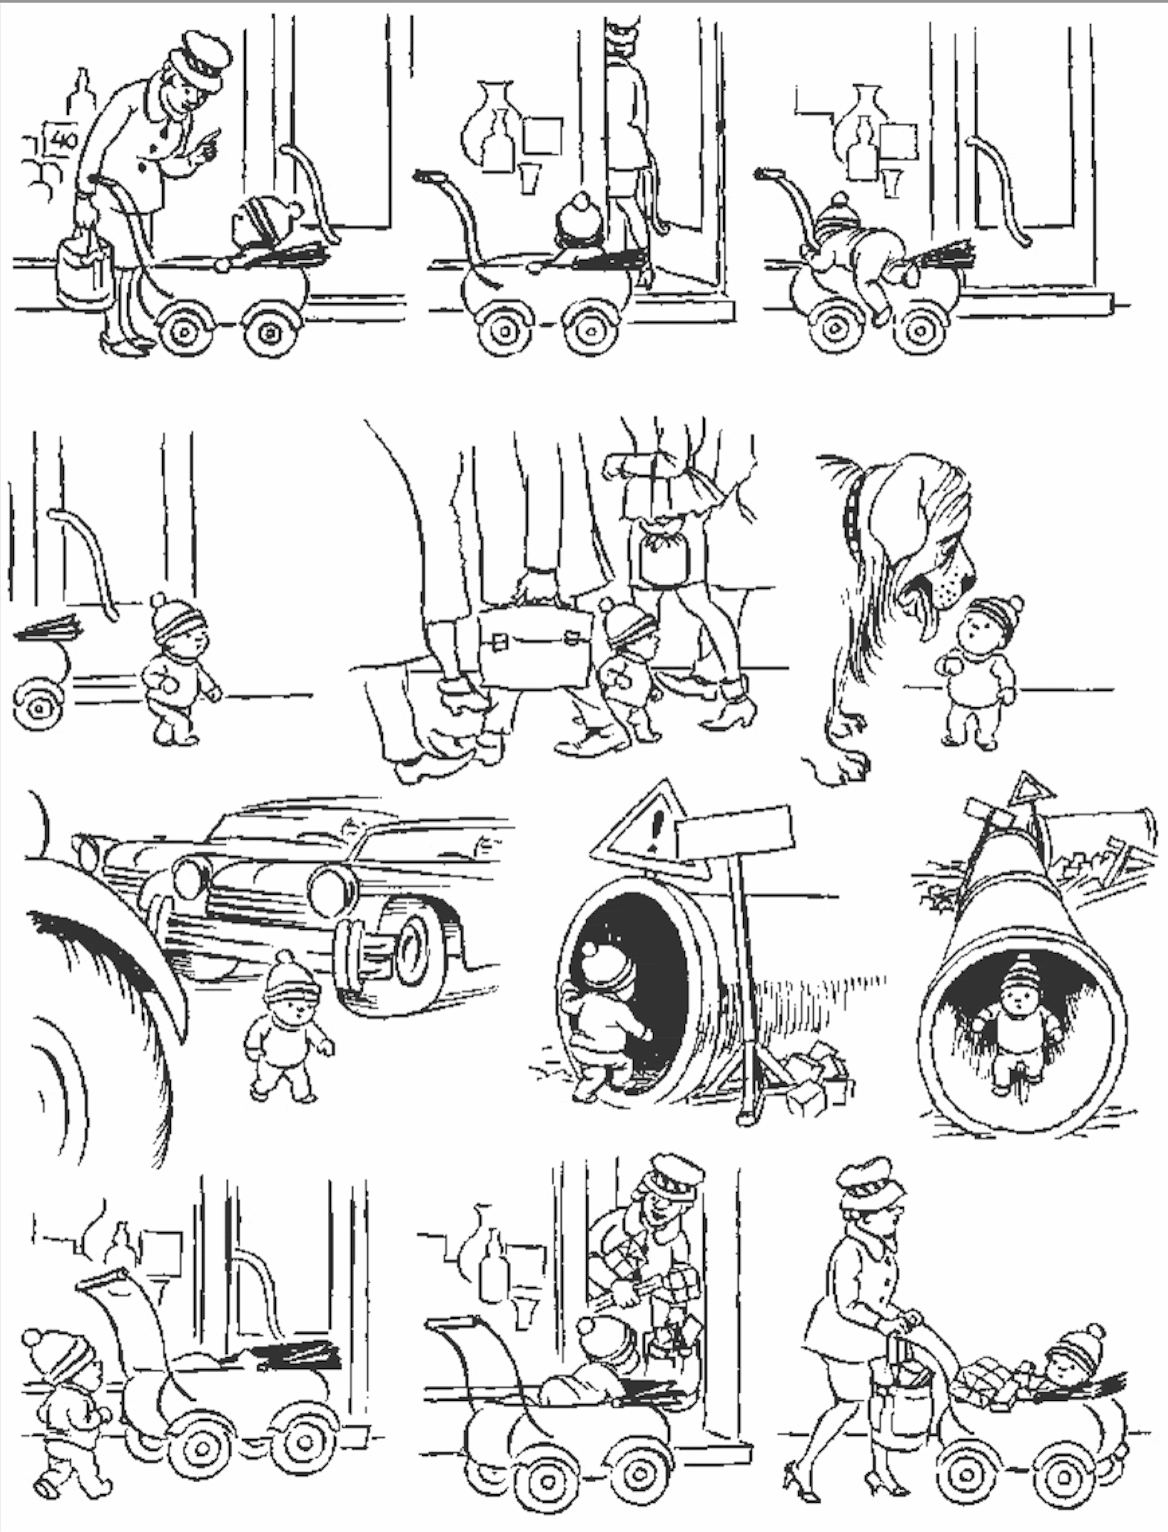
\includegraphics[width=\textwidth, center]{Figures/elicitation/adventure.png} 
\captionsetup{width=\textwidth}
\caption[Tasks: Adventure]{\label{fig:tasks:ad} The image used to elicit adventure task.}
\end{figure}

\begin{figure}[ht!]
    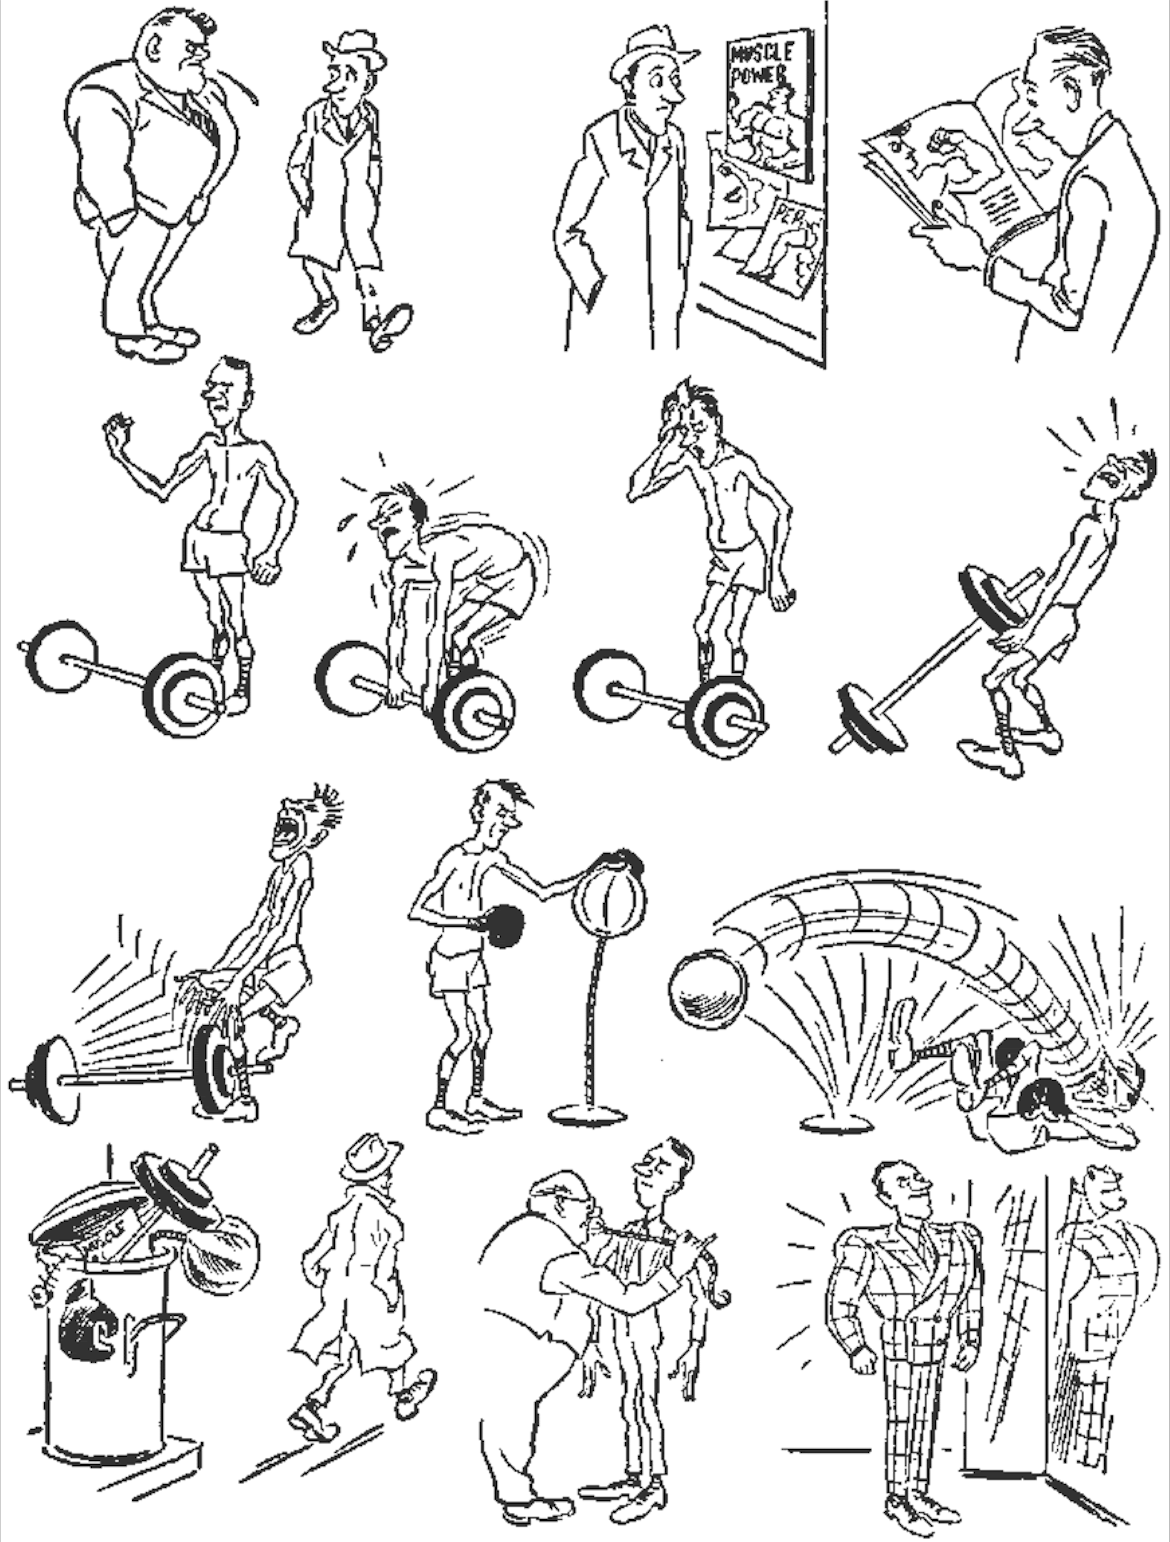
\includegraphics[width=\textwidth, center]{Figures/elicitation/sportsman.png} 
\captionsetup{width=\textwidth}
\caption[Tasks: Sportsman]{\label{fig:tasks:sp} The image used to elicit sportsman task.}
\end{figure}

\begin{figure}[ht!]
    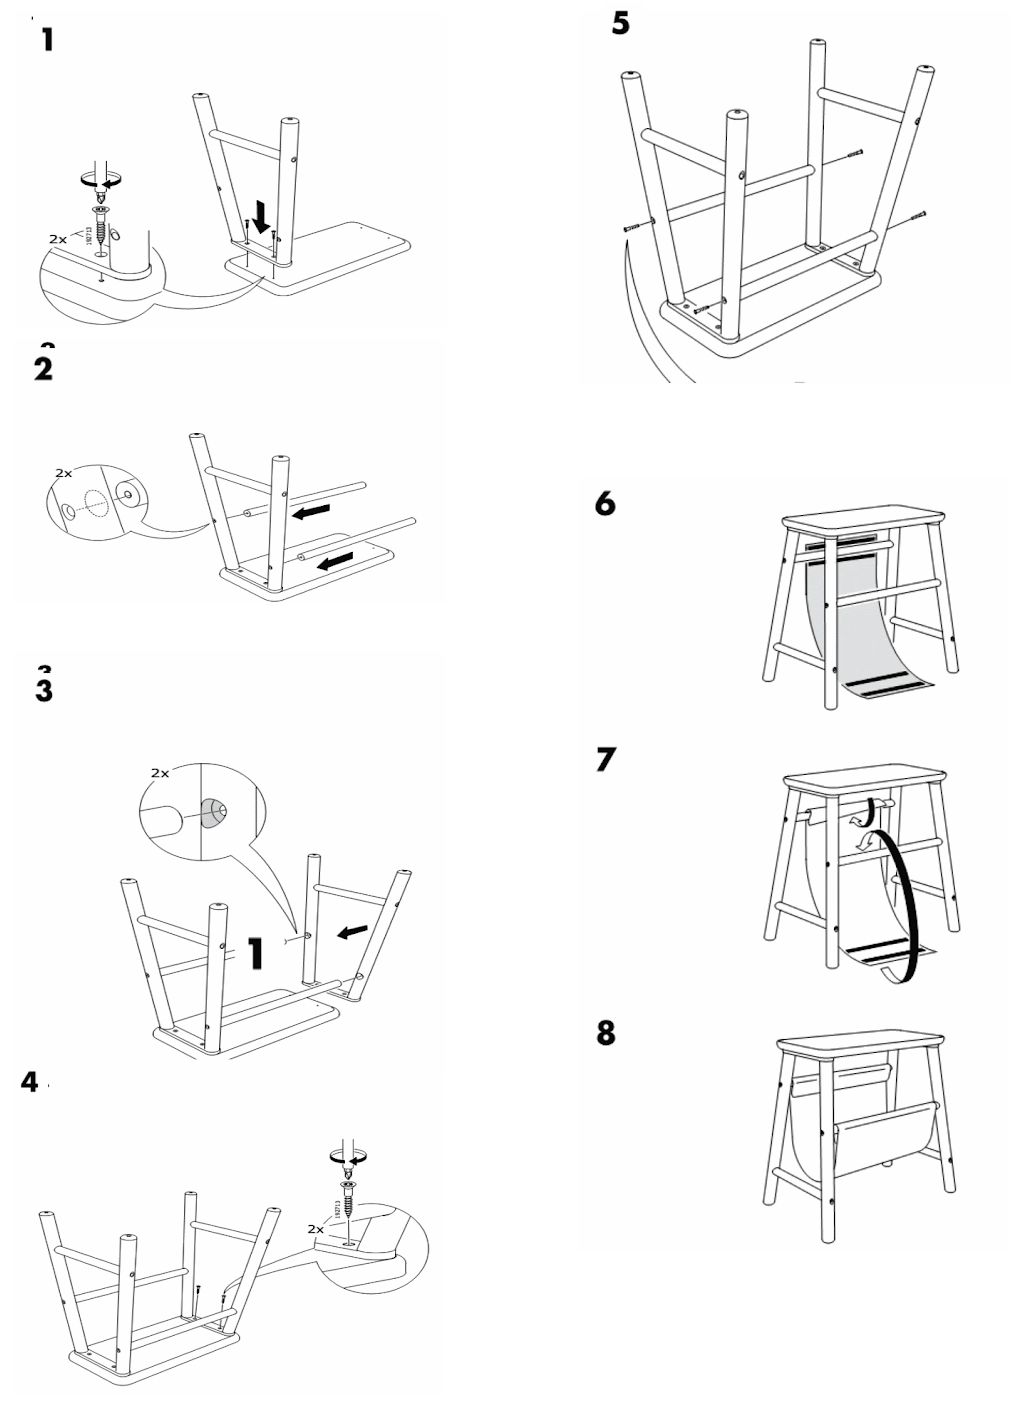
\includegraphics[width=\textwidth, center]{Figures/elicitation/chair.png} 
\captionsetup{width=\textwidth}
\caption[Tasks: Chair]{\label{fig:tasks:ch} The image used to elicit chair task.}
\end{figure}
\chapter{Clinical Data} % Main appendix title
\label{appendix:clincal_data} % For referencing this appendix elsewhere, use \ref{AppendixA}

\begin{table}[h!]
\begin{center}
\begin{tabular}{llllll}
\hline
    &     & \textbf{N} & \textbf{female} & \textbf{age}  & \textbf{edu\_years} \\ \hline
NAP &     & 31         & 25              & 27.13 (7.14)  & 13.32 (2.41)        \\
Dep &     & 18         & 18              & 20.89 (3.71)  & 12.67 (1.94)        \\
HC  & all & 127        & 89              & 40.42 (19.15) & 15.55 (2.54)        \\
    & psy & 41         & 31              & 27.62 (11.16) & 15.05 (2.07)        \\ \hline
\end{tabular}
\captionsetup{width=\textwidth}
\caption[Full Russian Clinical Dataset.]{\label{tab:data:ru:full_sample} Social statistics of the full Russian clinical dataset including the participants doing other tasks than the for selected. Standard deviation is provided in parenthesis for each mean value. ``edu\_years'' indicates years of education. ``Dep'' is the sample wit predominantly depressive symptoms. ``HC psy'' stands for the subset of the healthy patients for which a clinical impression and psychiatric assessment is available.}
\end{center}
\end{table}

\begin{table}[h]
\resizebox{\textwidth}{!}{%
\begin{tabular}{lllllllllllll}
\hline
\textbf{} & \textbf{sex} & \textbf{N} & \textbf{age}                      & \textbf{edu\_years}              & \textbf{Dep} & \textbf{TD} & \textbf{P\_N} & \textbf{PANSS\_TD} & \textbf{PANSS} & \textbf{PANSS\_n} & \textbf{PANSS\_p} & \textbf{PANSS\_o} \\ \hline
range       & & & & & & & &  4-28 & 30-210 & 7-49  & 7-49 & 16-112  \\ \hline
NAP       & all          & 31         & 27.13 (7.14)                      & 13.32 (2.41)                     & 0.58 (0.85)           & 0.84 (0.73)          & 29                        & 10.03 (3.74)       & 69.79 (16.13)  & 22.93 (8.59)        & 15.90 (4.92)        & 30.97 (8.42)      \\ \hline
          & f       & 25         & 27.80 (7.53)                       & 13.56 (2.48)                     & 0.72 (0.89)           & 0.8 (0.76)           & 23                        & 9.43 (3.62)        & 69.13 (15.38)  & 22.52 (7.79)        & 15.3 (4.91)         & 31.3 (9.08)       \\
          & m         & 6          & 24.33 (4.72)                      & 12.33 (1.97)                     & 0.0 (0.0)             & 1.0 (0.63)           & 6                         & 12.33 (3.56)       & 72.33 (20.16)  & 24.5 (11.93)        & 18.17 (4.67)        & 29.67 (5.65)      \\ \hline
Dep       & female       & 18         & 20.89 (3.71)                      & 12.67 (1.94)                     & 0.56 (0.62)           & 0.06 (0.24)          & 13                        & 4.42 (0.9)         & 37.92 (5.89)   & 8.31 (1.97)         & 8.46 (1.94)         & 21.15 (3.58)      \\ \hline
HC  & all          & 41         & 27.62 (11.16)                     & 15.05 (2.07)                     & 0.0                   & 0.0                  & 22                        & 4.36 (1.0)         & 30.77 (1.54)   & 7.23 (0.53)         & 7.23 (0.61)         & 16.32 (0.95)      \\ \hline
          & f       & 31         & 27.19 (10.59) & 15.23 (1.67) & 0.0                   & 0.0                  & 20                        & 4.4 (1.05)         & 30.85 (1.6)    & 7.25 (0.55)         & 7.25 (0.64)         & 16.35 (0.99)      \\
          & m         & 10         & 29.11 (13.57)                     & 14.5 (3.06)                      & 0.0                   & 0.0                  & 2                         & 4.0 (0.0)          & 30.0 (0.0)     & 7.0 (0.0)           & 7.0 (0.0)           & 16.0 (0.0)        \\ \hline
\end{tabular}
}
\captionsetup{width=\textwidth}
\caption[Full Russian Clinical Dataset: Psychiatric Scores]{\label{tab:data:ru:full_sample:psy} Clinical statistics of the psychiatric sample in the Russian clinical dataset including the participants doing other tasks than the for selected. Standard deviation is provided in parenthesis for each mean value. The range is provided for the possible values of the psychiatric scales. \\ ``HC'' only refers to the subset of the healthy patients for which a clinical impression and psychiatric assessment is available. ``f'' stands for female; ``m'' for male. ``edu\_years'' indicates years of education; ``Dep'' indicates clinical impression of depression severity varying from 0 to 3; ``TD'' indicates clinical impression of thought disorder severity varying from 0 to 3; ``P\_N'' indicates the number of participants for whom PANSS scores are available, ``PANSS\_td'' stands for the sum for PANSS questions related to formal thought disorder, ``PANSS\_neg'' stands for the negative PANSS sub-scale, ``PANSS\_pos'' for the positive sub-scale, and ``PANSS\_o'' for the general psychopathology sub-scale.}
\end{table}

\begin{table}[h!]
\begin{center}
\begin{tabular}{llll}
\hline
\textbf{} & \textbf{code} & \textbf{diagnosis}                                & \textbf{N} \\ \hline
NAP       & F20           & schizophrenia                                     & 20         \\
          & F25           & schizoaffective.disorder                          & 8          \\
          & F21           & schizotypal.disorder                              & 2          \\
          & F21.3         & schizotypal.disorder.pseudoneurotic.schizophrenia & 1          \\ \hline
Dep       & F31           & bipolar.affective.disorder                        & 6          \\
          & F60.31        & borderline.personality.disorder                   & 3          \\
          & F31.4         & bipolar.affective.disorder.severe                 & 2          \\
          & F31.5         & bipolar.affective.disorder.severe.psychotic       & 2          \\
          & F33           & recurrent.depressive.disorder                     & 2          \\
          & F32.1         & depressive.episode.moderate                       & 1          \\
          & F33.3         & recurrent.depressive.disorder.severe.psychotic    & 1          \\
          & F60           & personality.disorder                              & 1          \\ \hline
\end{tabular}
\captionsetup{width=\textwidth}
\caption[Russian Clinical Dataset: Diagnosis]{\label{tab:data:ru:sample:diagnosis} Diagnosis frequencies in the clinical samples.}
\end{center}
\end{table}

\begin{table}[h!]
\begin{center}
\begin{tabular}{lllllll}
\hline
    &     & adventure & chair & present & sportsman & table & bench & party & trip & winterday \\ \hline
NAP &     & 30        & 17    & 21      & 28        & 0     & 0     & 0     & 1    & 0         \\
Dep &     & 14        & 14    & 13      & 14        & 0     & 0     & 0     & 0    & 0         \\
HC  & all & 55        & 44    & 47      & 54        & 30    & 28    & 35    & 39   & 40        \\
    & psy & 25        & 16    & 19      & 26        & 0     & 0     & 7     & 9    & 12        \\ \hline
\end{tabular}
\captionsetup{width=\textwidth}
\caption[Russian Clinical Dataset: Task Availability]{\label{tab:data:ru:full_sample:tasks} Task availability for all tasks in Russian clinical dataset. ``Dep'' is the sample wit predominantly depressive symptoms. ``HC psy'' stands for the subset of the healthy patients for which a clinical impression and psychiatric assessment is available.}
\end{center}
\end{table}


%----------------------------------------------------------------------------------------


\end{document}  
